    %   Il progetto nasce dal template per il frontespizio realizzato da Marco Antonio Corallo, che ringrazio. Seguono alcuni commenti per evidenziare la presenza di alcuni pacchetti che mi sono stati utili per la stesura della tesi. Chiaramente, dipende tutto dal tipo di lavoro che uno vuole eseguire, che determina anche le diverse esigenze. Durante la stesura ho passato molto tempo su siti e forum a cercare di risolvere alcuni probelmi di formattazione, ma in generale Latex è stato piuttosto versatile. 

% Tipo di documento. L'uso di twoside implica che i capitoli inizino sempre con la prima pagina a sinistra, eventualmente lasciando una pagina vuota nel capitolo precedente. Se questa cosa è fastidiosa, è possibile rimuoverlo. 
\documentclass[a4paper, twoside,openright]{report}

\usepackage{[caption}
\usepackage{tikz}
%\usepackage{lineno}
\usepackage{notoccite}


% \usepackage[absolute,overlay]{textpos}
% \usepackage{onimage}
% Dimensione dei margini
\usepackage[a4paper,top=3cm,bottom=3cm,left=3cm,right=3cm]{geometry} 
% Dimensione del font
\usepackage[fontsize=13pt]{scrextend}
% Lingua del testo
\usepackage[english]{babel}
% Lingua per la bibliografia
\usepackage[square,sort,comma,numbers]{natbib}
% Codifica del testo
\usepackage[utf8]{inputenc} 
% Encoding del testo
\usepackage[T1]{fontenc}
\usepackage{caption}
\usepackage{subcaption}
% Permette di generare testo fittizio. Mi è stato utile 
% per capire quale sarebbe stata l'impostazione del 
% testo nella pagina prima che scrivessi un determinato paragrafo

% Per ruotare le immagini
\usepackage{rotating}
% Per modificare l'header delle pagine 
\usepackage{fancyhdr}     

% Librerie matematiche
\usepackage{amssymb}
\usepackage{mathrsfs}
\usepackage{amsmath}
\usepackage{amsthm}         

% Uso delle immagini
\usepackage{graphicx}
% Uso dei colori
%\usepackage[dvipsnames]{xcolor}         
% Uso dei listing per il codice
\usepackage{listings}          
% Per inserire gli hyperlinks tra i vari elementi del testo 
\usepackage{hyperref}     
% Diversi tipi di sottolineature


% -----------------------------------------------------------------

% Modifica lo stile dell'header
\pagestyle{fancy}
\fancyhf{}
\lhead{\leftmark}
\rhead{\textbf{\thepage}}
\fancyfoot{}
\setlength{\headheight}{12.5pt}

% Rimuove il numero di pagina all'inizio dei capitoli
\fancypagestyle{plain}{
  \fancyfoot{}
  \fancyhead{}
  \renewcommand{\headrulewidth}{0pt}
}


% Stile del codice
\lstdefinestyle{codeStyle}{
    % Colore dei commenti
    commentstyle=\color{black},
    % Colore delle keyword
    keywordstyle=\color{black},
    % Stile dei numeri di riga
    numberstyle=\tiny\color{black},
    % Colore delle stringhe
    stringstyle=\color{violet},
    % Dimensione e stile del testo
    basicstyle=\ttfamily\footnotesize,
    % newline solo ai whitespaces
    breakatwhitespace=false,     
    % newline si/no
    breaklines=true,                 
    % Posizione della caption, top/bottom 
    captionpos=b,                    
    % Mantiene gli spazi nel codice, utile per l'indentazione
    keepspaces=true,                 
    % Dove visualizzare i numeri di linea
    numbers=left,                    
    % Distanza tra i numeri di linea
    numbersep=5pt,                  
    % Mostra gli spazi bianchi o meno
    showspaces=false,                
    % Mostra gli spazi bianchi nelle stringhe
    showstringspaces=false,
    % Mostra i tab
    showtabs=false,
    % Dimensione dei tab
    tabsize=2
} \lstset{style=codeStyle}

% Stile di codice per dimensioni maggiori, in cui ho avuto bisogno di un testo più picolo (ad esempio se si vuole inserire del codice che ha linee molto lunghe). Per usare questo stile piuttosto che il precedente, usare 

% \lstset{style=longBlock}
%  % inserire il codice...
% \lstset{style=codeStyle}

% Il secondo comando consente di tornare allo stile precedente 
\lstdefinestyle{longBlock}{
    commentstyle=\color{teal},
    keywordstyle=\color{Magenta},
    numberstyle=\tiny\color{gray},
    stringstyle=\color{violet},
    basicstyle=\ttfamily\scriptsize,
    breakatwhitespace=false,         
    breaklines=true,                 
    captionpos=b,                    
    keepspaces=true,                 
    numbers=left,                    
    numbersep=5pt,                  
    showspaces=false,                
    showstringspaces=false,
    showtabs=false,                  
    tabsize=2
} \lstset{style=codeStyle}

% Togliendo il commento al comando che segue, si inseriscono nella bibliografia anche le fonti presenti in Bibliography.bib ma non citati direttamente con il comando \cite
% \nocite{*}

% Margini prima e dopo blocchi di codice, per avere più distanza
\lstset{aboveskip=20pt,belowskip=20pt}

% Modifica dello stile dei riferimenti, con il testo in cyano
\hypersetup{
    colorlinks,
    linkcolor=black,
    citecolor=black
}

% Aggiunti definizioni, teoremi, linea e listing
\newtheorem{definition}{Definizione}[section]
\newtheorem{theorem}{Teorema}[section]
\providecommand*\definitionautorefname{Definizione}
\providecommand*\theoremautorefname{Teorema}
\providecommand*{\listingautorefname}{Listing}
\providecommand*\lstnumberautorefname{Linea}

\raggedbottom

%\newcommand{\cgs}[1]{{\textcolor{brown}[\textcolor{red}{\bf{GS: }}{ \textcolor{brown}{#1]}}}}             
%\newcommand{\cmc}[1]{{\textcolor{blue}[\textcolor{magenta}{\bf{MC: }}{ \textcolor{blue}{#1]}}}}
\newcounter{apdxsection}
\newcommand\unappendix{\par
  \setcounter{apdxsection}{\value{section}}%
  \setcounter{section}{\value{savesection}}%
  \setcounter{subsection}{0}%
  \gdef\thesection{\@arabic\c@section}}
\setcounter{tocdepth}{4}
\setcounter{secnumdepth}{4}
% -----------------------------------------------------------------
\begin{document}

\begin{titlepage}
\begin{figure}[!htb]
    \centering
    
\includegraphics[keepaspectratio=true,scale=0.5]{figures/eps/cherubinFrontespizio.eps}
\end{figure}
\begin{figure}[!htb]
    \centering
    
\includegraphics[keepaspectratio=true,scale=0.5]{figures/eps/logo_pant541.eps}
\end{figure}

\begin{center}
    %\LARGE{University of Pisa}
    %\vspace{5mm} \\
     \Large{Department of Physics E. Fermi}
    \vspace{5mm}
    \\ \Large{Master's Degree in Physics}
\end{center}

\vspace{15mm}
\begin{center}
    {\LARGE{\bf Commissioning of the Mu2e\\ \vspace{3mm} Data Acquisition system and the\\ \vspace{5mm} Vertical Slice Test of the straw tracker}}
    
    % Se il titolo è abbastanza corto da stare su una riga, si può usare
    
    % {\LARGE{\bf Un fantastico titolo per la mia tesi!}}
\end{center}
\vspace{25mm}

\begin{minipage}[t]{0.47\textwidth}
	{\large{Supervisors:}{\normalsize\vspace{3mm}
	\bf\\ \large{Dr. Pavel Murat} \normalsize\vspace{3mm}\bf \\ \large{Prof. Simone Donati}}}
\end{minipage}
\hfill
\begin{minipage}[t]{0.47\textwidth}\raggedleft
	{\large{Candidate:}{\normalsize\vspace{3mm} \bf\\ \large{Sara Gamba}}}
\end{minipage}

\vspace{25mm}
\hrulefill
\\\centering{\large{Academic year 2023/2024}}

\end{titlepage}

\cleardoublepage
\thispagestyle{empty}
\vspace*{\stretch{1}}
\begin{flushright}
\itshape 
dediche
\end{flushright}
\vspace{\stretch{2}}
\cleardoublepage

\begin{abstract}
\noindent


The primary objective of the Mu2e experiment at Fermilab is to search 
for neutrino-less coherent $\mu \rightarrow e$ conversion in the field of an 
aluminum nucleus ($\mu^- \text{Al} \rightarrow e^- \text{Al}$). The signature 
of this process is a monochromatic conversion electron with an energy of 
approximately 104.97 MeV \cite{bartoszek2015mu2e}. Within the Standard 
Model, the branching ratio for this process, as well as for the $\mu \rightarrow e \gamma$ 
decay, including neutrino masses and oscillation, is expected to be of the order of $\mathcal{O}(10^{-54})$.


These values are far beyond current experimental capabilities.
However, models of physics beyond the Standard Model predict much higher relative rates,
approaching an observable level.
The SINDRUM II experiment 
set an upper limit on muon conversion at $7 \times 10^{-13}$ (90\% C.L.) on Au target 
\cite{SINDRUMII:2006dvw}, and the Mu2e collaboration aims to improve this limit by 
four orders of magnitude. Observing this process would provide a clear evidence of physics 
beyond the Standard Model.


Mu2e adopts a sophisticated experimental setup to achieve its goals. An 8.9 GeV proton 
beam from Fermilab strikes a tungsten target, producing muons through pion decays.
These particles are transported via a series of superconducting solenoids to an aluminum 
stopping target, where the conversion may occur. The system incorporates several 
components to accurately identify the conversion electrons and differentiate 
them from various backgrounds, including a straw tracker, an electromagnetic 
calorimeter, a Cosmic Ray Veto.


The tracker must provide excellent momentum resolution, approximately 1 MeV/c, 
to distinguish the monochromatic conversion electron signal from the background. 
To minimize energy loss, a straw tube tracker will be used \cite{bobbb}.


The detector has a modular design, consisting 
of basic elements referred to as $Panel$s, $Face$s, $Plane$s, and $Station$s. The 
tracker comprises panels containing arrays of straw tubes, which are the 
sensitive units, arranged like the harp chords.

This Thesis presents a comprehensive study of the Mu2e tracker, 
covering various aspects from initial commissioning to optimization and first 
steps of the calibration processes. My work at Fermilab has focused on the 
complete Data Acquisition (DAQ) testing from both hardware and software 
perspectives. I was involved in the commissioning of the Mu2e DAQ system and 
the Vertical Slice Test (VST) of the tracker. The VST encompasses the entire 
testing chain, from the straws to the readout, to processed data on disk.


Chapter \ref{commissioning} details the commissioning of the tracker 
DAQ system, emphasizing the importance of understanding the readout 
process before data acquisition. This includes validating the readout 
logic and firmware through Monte Carlo simulations to confirm functionality 
and buffering, monitoring data quality from the tracker preamplifiers and 
front-end electronics, and assessing overall DAQ performance to ensure 
reliability during future calibration and data-taking.


Given the high data volume expected during Mu2e operations, estimated 
at approximately 7 PBytes per year, optimizing memory usage and minimizing 
CPU consumption are critical. A significant challenge lies in effectively 
flagging $\delta$-electron hits, which are the primary source of hits in 
the tracker, without compromising the efficiency of conversion electron 
hit detection and track reconstruction. $\delta$-electrons originate from 
Compton scattered electrons, pair production electrons and positrons, and 
delta rays. Compton scattered electrons are produced when photons, from 
neutron capture, interact with the detector material. Typically, these 
photons have energies of a few MeV. Pair production electrons and positrons 
are generated during nuclear recoil processes. Delta rays 
are produced when high-energy charged particles collide 
with the detector material. A detailed study of pre-pattern recognition 
and a comparison of two algorithms for $\delta$-electron flagging is 
provided in Chapter \ref{delta} to address this issue.


Chapter \ref{planning} discusses the initial steps towards the calibration 
phase of the tracker. Our ultimate goal is to conduct a time calibration of 
the first assembled station of the tracker, aiming for a longitudinal 
position resolution better than 4 cm. This involves determining the signal 
propagation times and channel-to-channel delays using cosmic muons. The 
calibration will be conducted with a vertically oriented station due 
to technical constraints, and the impact of this orientation on trajectory 
reconstruction and potential biases is thoroughly analyzed. Together, 
these studies provide essential insights into the operation, optimization, 
and calibration of the Mu2e tracker system, contributing to its 
overall performance and reliability.


\end{abstract}


\tableofcontents

% Rimuovere se non si vuole la tabella delle figure
\listoffigures
\listoftables
\chapter{Charged Lepton Flavor Violation}
\textit{This Chapter offers a concise overview of the fundamental theoretical and experimental components essential to understand the objectives 
of the Mu2e experiment at Fermilab and the work conducted for this Thesis. The introduction to the Standard Model and certain extensions serves to 
justify the investigation of Charged Lepton Flavor Violation (CLFV), since it would be a clear signal of new physics beyond the current theories. 
Fundamental bibliography for this chapter can be found in Ref. \cite{Bernstein_2013} and \cite{clfv_signorelli}.}
\section{Theoretical Introduction}
\subsection{The Standard Model}
The Standard Model provides an excellent description of elementary particles and their interactions. It describes three out of 
four the fundamental forces known to this day: electromagnetism interaction, weak interaction and strong interaction. This theory is 
based on the Gauge symmetry group $U(1)_Y \times SU(2)_L \times SU(3)_C$. The first two terms describe the electroweak interaction, $Y$ indicates 
the hypercharge and $L$ refers to the fact that this acts only on the left handed components of the fields. The last term describes the strong interaction and $C$ indicates the color charge.
The Standard Model describes the elementary fields shown in Fig. \ref{fig:sm}.

\begin{figure}[!h]
\centering
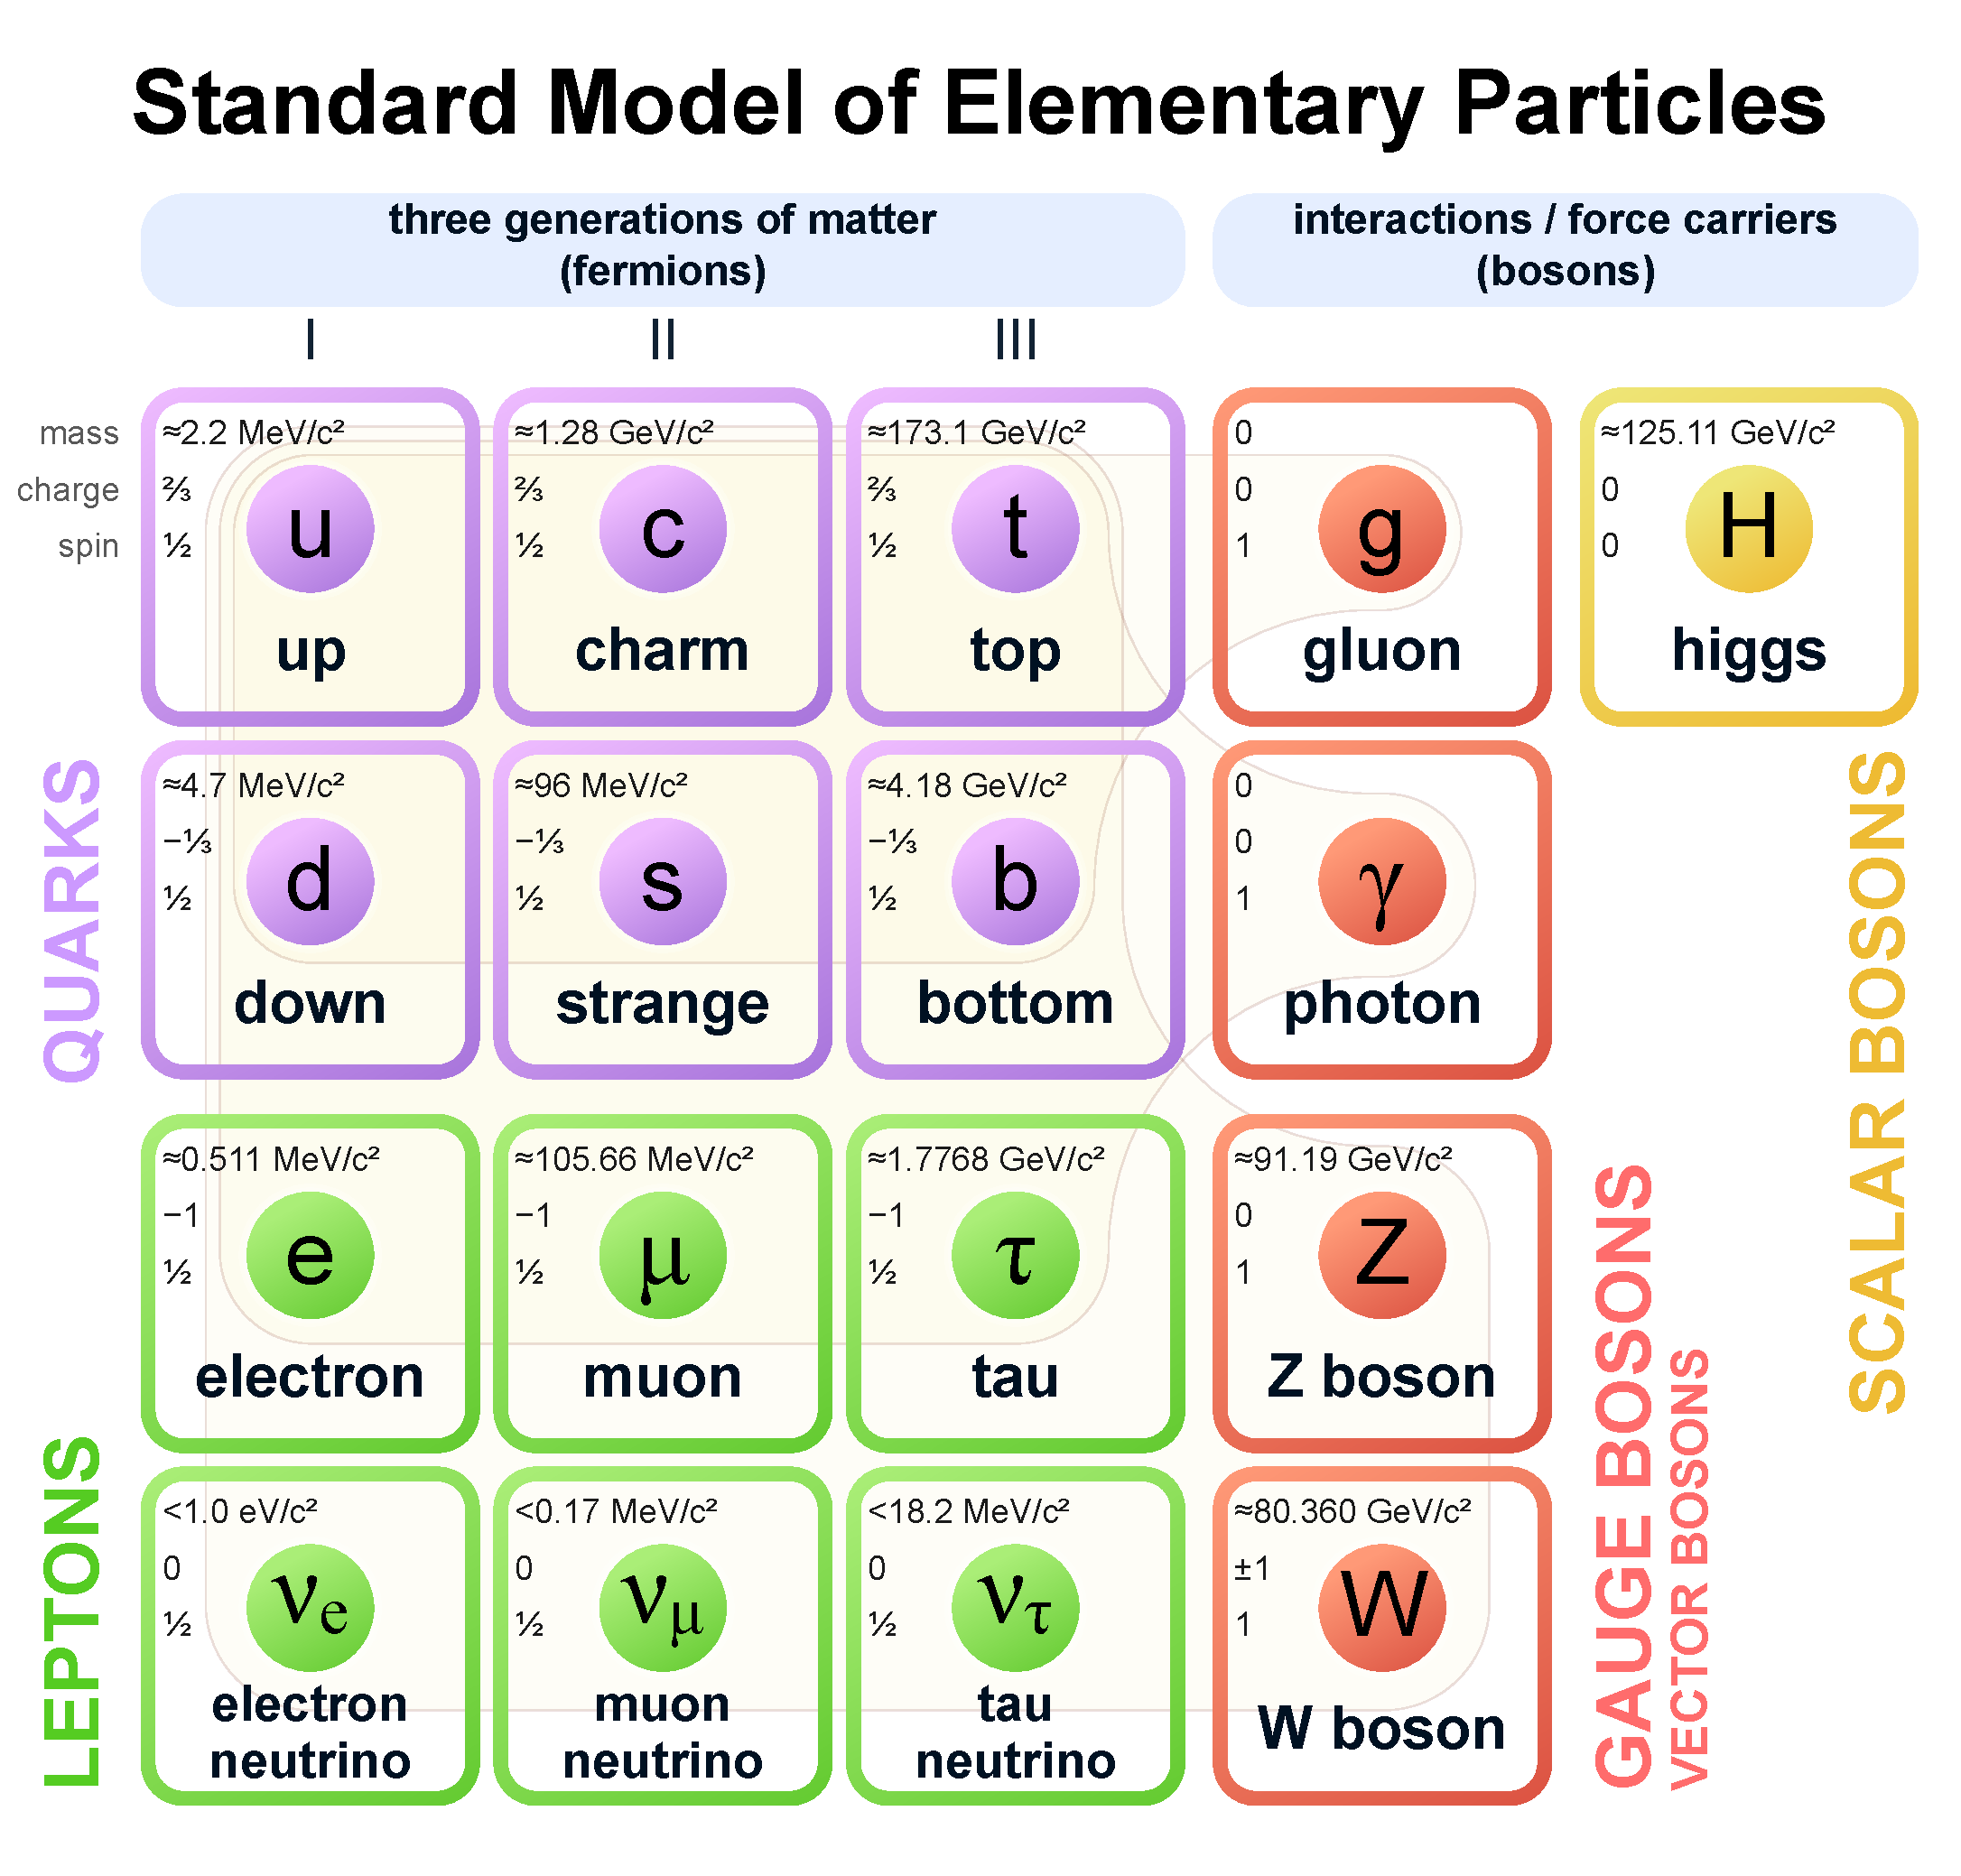
\includegraphics[width =0.8\textwidth]{figures/pdf/Standard_Model_of_Elementary_Particles.pdf}
\caption{Elementary particles of the Standard Model.}
\label{fig:sm}
\end{figure}


\subsubsection{Bosons}\label{bosons}
A boson is a particle with zero or integer spin, which follows Bose-Einstein statistics.
There are twelve fundamental bosons, that are the mediators of interactions as the $\gamma$, $Z$, $W^{\pm}$ for the electroweak interaction and as the eight gluons for the strong interaction.
The Higgs is a complex scalar weak isospin doublet that is responsible for the mechanism through which fermions and
bosons acquire mass and also explains the origin of $U (1)_{EM}$ through the spontaneous
symmetry breaking of the $SU (2)_L \times SU (1)_Y$ in the electroweak sector. Also mesons, that are composed of a quark and antiquark pair, are bosons. Bosons can be either massive, as $Z$, Higgs and $W^{\pm}$, or massless, as the photon and gluons.

\subsubsection{Fermions}
A fermion is a particle characterized by a non-integer spin, i.e. $1/2$, $3/2$ and follows the Fermi-Dirac statistics. 
The Pauli exclusion principle must be respected. Fermions are divided in two categories, leptons and quarks, depending 
on the forces through which they interact.  The arrangement of fermions into three generations is dictated by various 
properties, including mass among other properties, with more massive particles assigned to higher generations, as 
depicted in Fig.\ref{fig:sm}. Particles of the second and third generations exhibit instability and decay into first-generation 
particles. Leptons do not interact through strong interaction because they are not color charged, so they interact only via 
weak and electromagnetic interaction. They are categorized into two groups based on the electric charge: $e$, $\mu$, $\tau$ 
are the charged leptons and $\nu_e$, $\nu_{\mu}$, $\nu_{\tau}$ are the neutral ones. These particles form doublets of flavour. 
Neutrinos, due to their neutral nature, interact only weakly so their detection is extremely challenging. The six quarks 
participate in all known interactions. The known quarks are, in ascending order of mass and generation: up ($u$) and down 
($d$), strange ($s$) and charm ($c$), bottom ($b$), top ($t$) and their antiparticles. They primarily interact with each 
other through the strong force by gluons exchange. Free quarks have never been observed due to confinement, since they carry 
color charge. Confinement of quarks is a fundamental aspect of the theory of quantum chromodynamics (QCD) which describes the 
strong nuclear force. Quarks combine to form color-neutral particles known as hadrons, classified into baryons and mesons. 
Baryons consist of an odd number of quarks, while mesons, as mentioned in Subsection \ref{bosons}, are composed of a quark 
and an antiquark. Since quarks have weak electric charge and isospin, they can interact with each other and other fermions 
through weak and electromagnetic interactions.

\subsection{History of flavor}
The concept of flavor, namely the presence of three duplicates for every family of elementary fermions, is a fundamental aspect in particle physics. 
This principle is implemented within the Standard Model by introducing three copies of the Gauge representations of fermion fields. This view began 
to take shape in the late 1940s. The origin can be traced back to the experiment conducted by Conversi, Pancini and Piccioni in 1947. These experiment 
revealed that negative muons, called at that time $mesotrons$, did not undergo nuclear capture as expected. They decayed in electrons, similarly to positive muons, 
therefore they could not be Yukawa particles. In the same year, Powell and his group identified a two-step decay process ($\pi \rightarrow \mu \rightarrow e$), 
distinguishing the pion from the muon. Bruno Pontecorvo suggested that the muon could be a sort of $isomer$ of the electron, leading to the idea of a second 
generation of elementary fermions. Rochester and Butler discovered unusual events in cosmic rays pictures, later identified as $V-particles$ (later 
discovered that they originated from neutral kaons). This was the first hint of the existence of a second generation of quarks. In 1950 the search 
for decay $\mu \rightarrow e \gamma$ began. This decay was not found, leading to the principle of conservation of leptons. On the hadron side, 
the second generation of quarks was established in the mid-70s, involving the GIM mechanism and the discovery of the charm quark. Meanwhile, 
on the leptonic side, the upper limit on the branching ratio of $\mu^+ \rightarrow  e^+ \gamma$ was set in 1955. The discovery of parity violation 
in the late 1950s suggested the weak interaction is mediated by bosons. Feinberg started thinking that $\mu^+ \rightarrow  e^+ \gamma$ could occur 
at a level of $10^{-4}$ if the bosons existed, through a loop with neutrino and a boson. This lead to the two-neutrino hypothesis, suggesting that 
the neutrino coupled to the muon differs from that coupled to the electron, thereby prohibiting $\mu^+ \rightarrow  e^+ \gamma$. The existence of 
two neutrinos was verified at Brookhaven National Laboratory, with the scattering of two neutrinos coming from $\pi$, that produced only muons. 
After the observation of CP violation in neutral kaon decay, a third generation of quarks was hypothesized. After the discoveries of the $\tau$ (1976), 
the $b$ quark (1977), $t$ quark (1995) and $\nu_{\tau}$ (2000), a complete picture was achieved and the concept of flavor was consolidated in the Standard Model.


\subsection{Overview of CLFV}
There are three different lepton flavors: the electron-lepton $L_e$, the muon-lepton $L_{\mu}$ and the tau-lepton $L_{\tau}$. In Table \ref{tab:leptons}, the quantum numbers assigned to each lepton are displayed.
 \begin{center}  
\begin{table}[!h]
\centering
\renewcommand{\arraystretch}{1.5}
\begin{tabular}{c c c c}
\hline
Lepton & $L_e$ & $L_{\mu}$ & $L_{\tau}$\\
\hline
$e^-/e^+$ & $+1 \ /-1$ & 0 & 0 \\
$\nu_{e}/\bar{\nu}_{e}$ & $+1 \ /-1$ & 0 & 0 \\
$\mu^-/\mu^+$ & 0 & $+1 \ /-1$ & 0 \\
$\nu_{\mu}/\bar{\nu}_{\mu}$ & 0 & $+1 \ /-1$ & 0 \\
$\tau^-/\tau^+$ & 0 & 0 & $+1 \ /-1$\\
$\nu_{\tau}/\bar{\nu}_{\tau}$ & 0 & 0 & $+1 \ /-1$ \\
\hline
\end{tabular}
\caption{Lepton numbers assigned to neutrinos and charged leptons.}
\end{table}\label{tab:leptons}
\end{center}
In the Standard Model (SM) defined with massless left-handed neutrinos, Lepton Flavor (LF) is a conserved quantity, Ref. \cite{universe8060299}. Experimental observations have demonstrated that, as they travel, neutrinos exhibit flavor oscillations, which implies that they must have non-zero masses and mixing angles. This phenomenon represents also a violation of the conservation of the lepton flavor. The Standard Model, while successful in many aspects, fails to explain phenomena like neutrino masses and the consequent flavor oscillations. Since neutrinos get their masses through renormalizable Yukawa interactions
with the Higgs, the predicted CLFV transitions are suppressed by sums over $(\Delta m^2_{i j}/M^2 _W)^2$, as calculated in Ref. \cite{MARCIANO1977303} and as shown in Section \ref{massiveneutrinos}, where $\Delta m^2_{ij}$ is mass-squared difference between the neutrino mass eigenstates $i$, $j$ and $M_W$ is the $W$ boson mass. The neutrino mass difference is very small ($\Delta m^2 _{i j} \leq 10^{-3}$ eV$^2$) with respect to the $W$ boson mass so the expected branching ratios reach unmeasurable values, below $10^{-50}$. Experimental studies of the lepton flavor violating process could open a window to new physics. Moreover, lepton flavor constitutes an accidental symmetry within the SM, not related to the Gauge structure of the theory but coming
from its particle content, especially from the absence of RH neutrinos. Minor deviations from the Standard Model can easily give rise to extra occurrences of lepton flavor violation, leading to notable rates of CLFV.
There are various extensions of the Standard Model that could potentially be examined in the upcoming experimental searches for CLFV, that I will report in the next sections.
\subsection{Lepton sector in Standard Model}\label{leptonsector}
In the SM, only one Higgs field $\Phi$ exists. The fermions masses and the mixing term arise from the couplings of fermions with Higgs field. In the following, I will call the left-handed $i$-th quarks doublets and leptons doublets as $Q_{L,i}=(u_{L,i} \ d_{L,i})^T$ and $L_{L,i}=(\nu_{L,i} \ e_{L,i})^T$: $u_i$ will be the up-type quark, $d_i$ the down-type quark, $\nu_i$ the neutrino and $e_i$ the charged lepton. These are $SU(2)$ doublets, while $u_{R,j}$, $d_{R,j}$ and $e_{R,j}$ will be the right-handed up-type, down-type quarks and the right charged lepton of the $j$-generation respectively. There is no right-handed neutrino. The Yukawa coupling of fermions with the Higgs field $\mathscr{L}_Y$ is the sum of two terms: $\mathscr{L}_e$ that describes the leptonic component (Eq.\ref{leptoniccomponent}) and $\mathscr{L}_q$ that describes the quark one (Eq.\ref{quarkcomponent}).
\begin{equation}\label{leptoniccomponent}
    -\mathscr{L}_e=\left(Y_e\right)_{i j} \bar{L}_{L i} e_{R j} \Phi+ \text{ h.c. }
\end{equation}
\begin{equation}\label{quarkcomponent}
        -\mathscr{L}_q=\left(Y_u\right)_{i j} \bar{Q}_{L i} u_{R j} \widetilde{\Phi}+\left(Y_d\right)_{i j} \bar{Q}_{L i} d_{R j} \Phi+\text { h.c. }
\end{equation}

where the term $Y_f \ (f  =  u,d,e)$ describe the 3$\times$3 Yukawa complex matrices. $\widetilde{\Phi} \equiv i \tau_2 \Phi^*$ is the conjugate Higgs field. The mass terms of fermions, characterized by the $m_f \bar{f}_L f_R$ form, originate from the breaking of the $SU(2)_L \times U(1)$ symmetry caused by the vacuum expectation value of the Higgs field, as in Eq.\ref{higgs}.
\begin{equation}\label{higgs}
\langle\Phi\rangle=\frac{1}{\sqrt{2}}\left(\begin{array}{l}
0 \\
v
\end{array}\right) \qquad v \simeq 246 \mathrm{GeV}
\end{equation}
The fermion mass is given by:
\begin{equation}
\left(m_f\right)_{i j}=\frac{v}{\sqrt{2}}\left(Y_f\right)_{i j} \qquad f=u, d, e
\end{equation}
Since a right-handed neutrino does not appear in the Lagrangian, neutrinos have no mass, as it is formulated in the SM. The Yukawa matrices can be diagonalized 
through unitary rotations of the fields, as it follows:
\begin{equation}\label{bbbb}
Y_f=V_f \hat{Y}_f U_f^{\dagger} \qquad f=u, d, e
\end{equation}
where $ \hat{Y}_f $ is the diagonal Yukawa matrix. It is possible to label fermions in the rotated basis as $f^{\prime}$, so $f_L=V_f f^{\prime}_L$ and $f_R=V_f f^{\prime}_R $. Since $V_f$ and $U_f$ are unitary, the rotation will not affect the neutral interactions term and the kinetic terms, as we can see in $\bar{f}_L \gamma^\mu f_L=\bar{f}_L \gamma^\mu\left(V_f^{\dagger} V_f\right) f_L=\bar{f}_L^{\prime} \gamma^\mu f_L^{\prime}$. The coupling between fermion and Higgs boson will be:
\begin{equation}
-\mathscr{L}_{h \bar{f} f}=\frac{(\hat{m}_f)_{i j}}{v} \bar{f}_{L i}^{\prime}f^{\prime}_{R j} h+\text{h.c.} \qquad f=u, d, e
\end{equation}
where $\hat{m}_f$ denotes the diagonalized mass matrix: it is clear that there are no flavor-violating terms.
In quark sector flavor-violation arises from the rotations in Eq.\ref{bbbb} in the charged-current interactions with the $W$ bosons:
\begin{equation}\label{quarkviolation}
\begin{array}{c}
      { \displaystyle 
\mathscr{L}_{C C}  =\frac{g}{\sqrt{2}}\left(\bar{u}_L \gamma^\mu d_L+\bar{\nu}_L \gamma^\mu e_L\right) W_\mu^{+}+\text {h.c.} }\\
 {\displaystyle=\frac{g}{\sqrt{2}}\left(\bar{u}^{\prime}_L \gamma^\mu\left(V_u^{\dagger} V_d\right) d_L^{\prime}+\bar{\nu}^{\prime}_L \gamma^\mu\left(V_\nu^{\dagger} V_e\right) e_L^{\prime}\right) W_\mu^{+}+\text {h.c.}}
\end{array}
\end{equation}

The violation comes from the fact that $V_u \neq V_d$. The mixing is controlled by the Cabibbo-Kobayashi-Maskawa matrix $V_{CKM}\equiv V^{\dagger}_u V_d $, Ref. \cite{PhysRevLett.10.531}. Meanwhile, as the lepton sector contains massless neutrinos, $V_{\nu}$ can be arbitrarily chosen as $V_{\nu}=V_e$. From the preceding discussions, it becomes evident that in the SM with massless neutrinos, there is no occurrence of LFV in any form. The Lagrangian $\mathscr{L}_Y$ is invariant under three indipendent global $U(1)$ rotations, resulting in the conservation of three lepton family numbers: $L_e$, $L_\mu$ and $L_\tau$. Furthermore, if the Yukawa coupling Lagrangian includes supplementary terms involving the lepton fields, flavor violation can occur in the lepton sector. Examples of such additions could be a neutrino mass term or a second Higgs doublet.

\subsection{CLFV in the Standard Model with massive neutrinos}\label{massiveneutrinos}
The first evidence against the hypotesis of massless neutrinos emerged with the solar neutrino problem. In the 1960s, the solar neutrino detection experiment at Homestake revealed that the observed number of solar neutrinos, generated by fusion in the Sun, was significantly lower than the anticipated value based on the standard solar model, given that the detector was only sensitive to $\nu_e$, Ref. \cite{PhysRevLett.20.1205}. Consistent results were replicated in subsequent experiments employing radiochemical and Cherenkov detectors, discovering neutrino oscillations. These oscillation firmly established non-zero neutrino masses. The lepton flavor-violating neutrino oscillations showed that the global $U(1)$ symmetries associated with the lepton family numbers are not fundamental symmetries. A correction to standard model is needed to include neutrino mass terms. This is possible adding a right-handed neutrino singlet $\nu_R$ or some non-renormalizable operators.
\\
In the first case, an additional term $\Delta \mathscr{L}_D$ to the Yukawa coupling should be introduced:
\begin{equation}
-\Delta \mathscr{L}_D=\left(Y_\nu\right)_{i j} \bar{L}_{L i} \nu_{Rj} \widetilde{\Phi}+\text { h.c. }
\end{equation}
Similarly to other fermions, a Dirac mass term $m_{\nu} \bar{\nu}_L \nu_R$ is generated through simmetry breaking:
\begin{equation}
\left(m_\nu^D\right)_{i j}=\frac{v}{\sqrt{2}}\left(Y_\nu\right)_{i j}
\end{equation}
In this case, the small neutrino masses can be explained only if a very small term $Y_\nu$ is considered ($\leq 10^{-12}$), Ref. \cite{clfv_signorelli}. This brings us considering the second hypotesis: adding non-renormalizable operators can introduce Majorana masses for left-handed neutrinos alone. The corresponding $\Delta \mathscr{L}_M$ can be written as:
\begin{equation}
-\Delta \mathscr{L}_M=\frac{1}{2}\left(m_\nu^M\right)_{i j} \overline{\nu_{L i}^C} \nu_{L j}+\text{ h.c.}
\end{equation}
where $\overline{\nu_{L }^C} $ is the charge-conjugated fields. This term violates lepton number and requires an operator of dimension 5, Ref. \cite{wein}, to be consistent with SM symmetries. A minimal Lagrangian is given by:
\begin{equation}
-\Delta \mathscr{L}_{M \text { eff}}=\frac{\mathcal{C}_{i j}}{\Lambda}\left(\overline{L_{L i}^C} \tau_2 \Phi\right)\left(\Phi^T \tau_2 L_{L j}\right)+\text { h.c.}
\end{equation}
where the $\Lambda$ term represents a mass scale characteristic of extra degrees of freedom and the $C_{ij}$ is an antisymmetric charge conjugation matrix. The corresponding Majorana mass term is:
\begin{equation}
\left(m_\nu^M\right)_{i j}=\frac{\mathcal{C}_{i j} v^2}{\Lambda}
\end{equation}
In this case, the small neutrino masses can be explained only if $\Lambda > > v$: this seems to appear more natural than the previous case. No matter how the extra neutrino mass factor is expressed precisely, a physical basis diagonalizing the mass matrix is determined, resulting in $V_{\nu} \neq V_e$ in Equation \ref{quarkviolation}. Lepton mixing is described by $U_{PMNS} \equiv V_{\nu}^{\dagger} V_e$, which is similar to the CKM matrix. The Pontecorvo-Maki-Nakagawa-Sakata (PMNS) matrix is the term that is typically used to refer to it. As it is in the basis diagonalizing charged lepton masses and it diagonalizes the neutrino mass matrix, $U_{PMNS}$ also explains the mixing between neutrino flavor eigenstates $\nu_{\alpha}$ and mass eigenstates $\nu_i$:
\begin{equation}
\nu_\alpha=\sum_{i=1,2,3}\left(U_{\mathrm{PMNS}}\right)_{l i} \ \nu_i \qquad l=e, \mu, \tau
\end{equation}
In addition to the neutral LFV observed in neutrino oscillations, the mixing outlined by $U_{PMNS}$ can in principle give rise to processes known as Charged Lepton Flavor Violations, i.e. LFV that involves charged leptons. The new Feynman diagrams are loops involving neutrinos and $W$ bosons, as $\mu \rightarrow e \gamma$ in Fig.\ref{fig:mutoegamma} and $\mu N \rightarrow e N$ in Fig.\ref{fig:mutoeN}. 



\begin{figure}[!h]
     \begin{subfigure}[b]{0.4\linewidth}
         \centering
         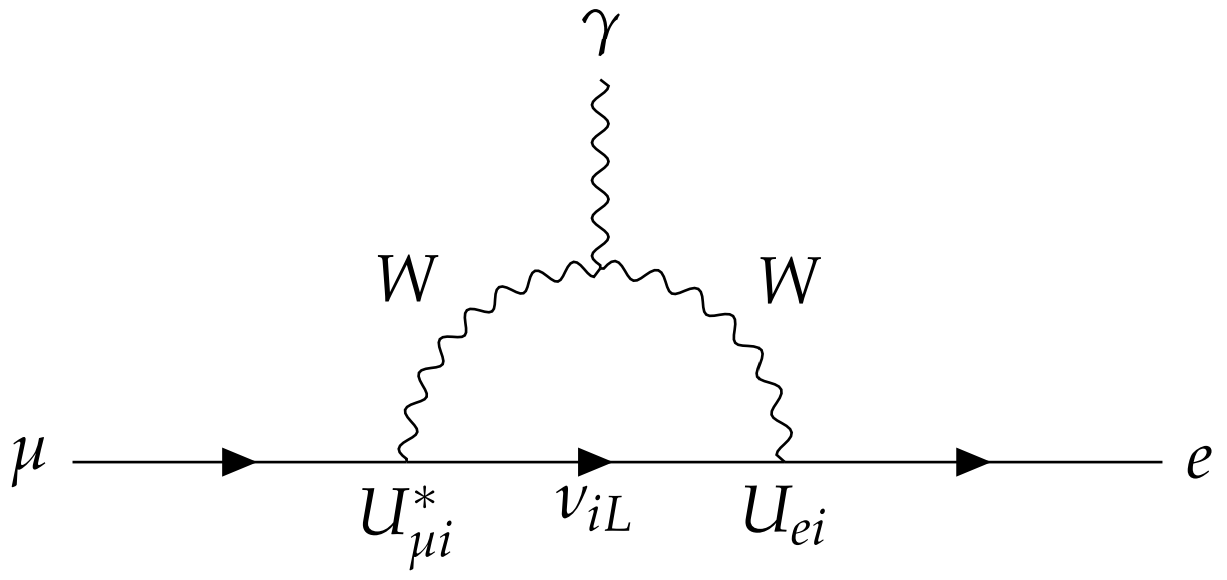
\includegraphics[scale = 0.2]{figures/png/Screenshot_20240217_171058.png}
         \subcaption{$\mu \rightarrow e \gamma$ process, Ref. \cite{universe8060299}.}
         \label{fig:mutoegamma}
     \end{subfigure}
     \begin{subfigure}[b]{0.7\linewidth}
         \centering
         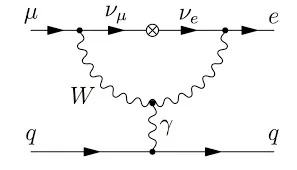
\includegraphics[scale = 0.5]{figures/jpg/1_erkKoywyuFzJmMv4PKpc9Q.jpg}
         \subcaption{$\mu N \rightarrow e N$ process.}
         \label{fig:mutoeN}
     \end{subfigure}
     \caption{Some of CLFV processes.}
        \label{fig:three graphs2}
\end{figure}
In the SM, each of these mechanisms is significantly inhibited. Using the example of $\mu \rightarrow  e \gamma $, the branching ratio of this process may be computed as follows:

\begin{equation}\label{br}
\begin{aligned}
B R(\mu \rightarrow e \gamma) & =\frac{3 \alpha}{32 \pi}\left|\sum_{i=2,3} U_{\mu i}^* U_{e i} \frac{\Delta m_{1 i}^2}{M_W^2}\right|^2 \\
& =\frac{3 \alpha}{32 \pi}\left(\frac{1}{4}\right) \sin ^2 2 \theta_{13} \sin ^2 \theta_{23}\left|\frac{\Delta m_{13}^2}{M_W^2}\right|^2
\end{aligned}
\end{equation}

where $\alpha$ is the fine structure constant, $U_{\mu i}$ and $U_{ei}$ are corresponding elements in the PMNS matrix, $\Delta m_{1i}^2$ are the neutrino squared mass differences, $M_W$ is the $W$ boson mass and $\theta_{13}$ and $\theta_{23}$ are rotating angles in PMNS matrix parametrization. The expression yields $B R(\mu \rightarrow e \gamma) \sim \mathcal{O}(10^{-54})$. The big discrepancy in mass between neutrinos and the $W$ boson results in an extraordinarily small value for $|\Delta m_{13}^2/M_W|$. Equivalent suppression mechanisms are evident in other CLFV processes. The rates predicted by the Standard Model are extremely small, making them impractical for detection in any experiment. On the other hand, numerous Beyond the Standard Model (BSM) theories incorporate mechanisms that substantially amplify CLFV rates, a topic to be addressed in the subsequent section. The small value of SM CLFV rates implies that the detection of any CLFV processes in experiments would unequivocally indicate the presence of physics beyond the SM.
\subsection{Beyond the Standard Model}
Numerous Beyond the Standard Model (BSM) theories propose mechanisms that could contribute to CLFV processes, potentially yielding detectable rates in experiments. Here, we highlight a selection of BSM theories known for their CLFV contributions. It is important to note that this list is not comprehensive; for further studies, additional reviews are available in Ref. \cite{clfv_signorelli} and Ref. \cite{universe8060299}.
\subsubsection{CLFV in Supersymmetry}\label{susy}
Supersymmetry (SUSY) is a theoretical framework that has oriented experiments in the CLFV reasearch for many years. On one hand, models with SUSY broken at energies close to electro-weak scale have given solution to the hierarchy problem, i.e. how to maintain the Higgs mass significantly smaller than the Planck scale ($\sim$10$^{19}$ GeV). On the other hand, the suppression of CLFV processes is due to the wide separation of the neutrinos and $W$ masses, which can be mitigated by introducing SUSY partners of neutrinos and $W$ bosons. This suggests that CLFV processes should have been observable earlier, unless SUSY breaking occurs at or near the electroweak scale ($\sim 10^2$ GeV), Ref. \cite{clfv_signorelli}. In this framework, each elementary particle has a superpartner,  with the same quantum numbers except for spin: a boson is the superpartner of a fermion and vice versa. A superpartner of a lepton is called $slepton$. If there is no common eigenstate base between lepton and $slepton$'s mass matrices then a physical $slepton$ will be a superposition of flavors. In this case a loop diagram can lead to CLFV, as shown in Fig.\ref{fig:susy}. Despite the similar topology to that of the SM contribution (Fig.\ref{fig:mutoegamma}), the typical SUSY mass is expected to be much higher than that of the neutrinos. Predictions for the branching ratio of this process vary among different SUSY models, contingent upon specific mechanisms and particle masses. These rates can undergo significant enhancement. For example, in an $SU(5)$ SUSY grand unified theory, the computed branching ratio could reach $\mathcal{O}(10^{-14})$ for a slepton mass on the order of $\mathcal{O}(10^{-14}$ GeV/c$^2)$, a value measurable for upcoming experiments.

\begin{figure}[!h]
\centering
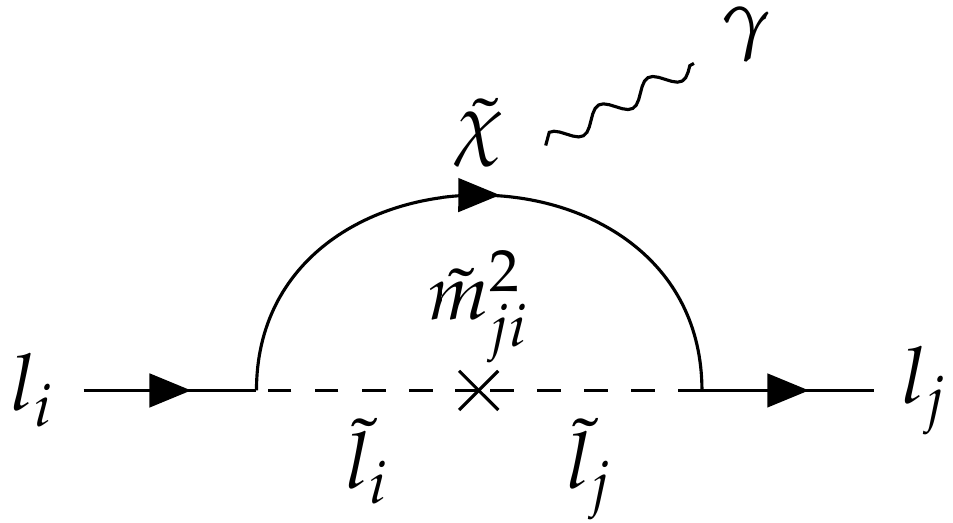
\includegraphics[width =0.4\textwidth]{figures/png/Screenshot_20240218_105920.png}
\caption{SUSY contribution to $l_i \rightarrow l_j\gamma$, through $sleptons$ mass mixing, Ref. \cite{universe8060299}.}
\label{fig:susy}
\end{figure}


\subsubsection{Two Higgs Doublet Model}\label{2higgs}
Although the Standard Model (SM) incorporates only one Higgs boson, there are no constraints against the presence of additional Higgs fields. One straightforward example of a comprehensive theory featuring multiple Higgs fields is the type III two Higgs doublet model (2HDM), where two Higgs bosons exist, each interacting with fermions and possessing a vacuum expectation value, Ref. \cite{Harnik_2013}. Generally, the Lagrangian incorporating extra Higgs fields post-electroweak symmetry breaking can be written as:
\begin{equation}
-\mathscr{L}=m_i \bar{f}_{L i} f_{R i}+\left(Y^\alpha\right)_{i j} \bar{f}_{L i} f_R{ }_j h^\alpha+\text { h.c. }+\ldots
\end{equation}
Non renormalizable terms of higher dimensions are omitted. $(Y^\alpha)_{i j}$ represents couplings to a single scalar field and the contributions from different Higgses are summed over. The non-zero-off-diagonal terms in $(Y^\alpha)_{i j}$ give rise to flavor violating Yukawa couplings. From accelerator and precision experiments, constraints on the off-diagonal coupling of the 125 GeV Higgs boson can be obtained.
\subsubsection{Leptoquark Models}
Leptoquarks (LQs) are theoretical particles initially proposed within the Pati-Salam model, Ref. \cite{PhysRevD.10.275}. Each LQ is linked to both baryon number ($B$) and lepton number ($L$). In various LQ models the quark and lepton sectors are unified. This unification allows for direct coupling between quarks and leptons via the exchange of LQs. Consequently, specific CLFV processes like $K_L^0 \rightarrow e \mu$ and $\mu N \rightarrow e N$ are mediated by LQs. Constraints on LQ models arise from both collider experiments and rare decay searches. Direct searches at ATLAS and CMS have excluded scalar LQs of the first and second generations with masses below $\sim$1 TeV. Indirect searches provide constraints on the mass-coupling plane, where regions with higher couplings and lower LQ masses correspond to higher branching ratios. Additionally, LQ models must satisfy constraints related to proton stability, as some models involve LQs that could mediate proton decay. To mitigate this, the corresponding LQs must either have extremely high masses or their related couplings must be exceedingly small, Ref. \cite{DORSNER20161}.
\subsubsection{Additional Neutral Gauge Boson}
Grand unified theories (GUTs) are constructed based on extended Gauge groups in the pursuit of a more fundamental model. At lower energies, these extended Gauge groups are believed to break down to the direct product of the Standard Model (SM) Gauge group $SU(3) \times SU(2) \times U(1)$ along with an additional $U(1)$ factor. The neutral Gauge boson associated with this $U(1)$ group can mix with the original SM neutral Gauge boson, resulting in two mass eigenstates, namely $Z$ and $Z'$. Additionally, extended Gauge theories require the introduction of additional fermion fields to cancel anomaly-free currents beyond those of $SU(5)$. These $new$ fermions can mix with the known SM fermions possessing the same electric and color charges, consequently affecting their couplings with Gauge bosons. The appearance of off-diagonal terms in neutral current couplings to fermions can lead to flavor-changing couplings to $Z$ and $Z'$. Certain CLFV processes, such as $\mu \rightarrow eee$ and $\mu-e$ conversion, receive tree-level contributions through intermediate $Z$ and $Z'$ bosons. Further insights into the phenomenology of the $Z'$ boson can be found in, Ref. \cite{Leike_1999}. The search for the existence of $Z'$ bosons is conducted through channels like $Z' \rightarrow \bar{f}f$ at hadron colliders. Mass lower limits of $Z'$ from various specific models are listed in Ref. \cite{zyla}, primarily falling within the low TeV range. Particularly, mass lower limits reported in CLFV final states $e\mu$, $e\tau$ and $\mu\tau$ range between 3.5 TeV and 4.5 TeV. Upper limits of $Z \rightarrow l_1 l_2$ couplings to the normal $Z$ boson are also provided in Table \ref{tab:upperlimits}.
%Quello che segue è un esempio di codice. E' possibile modificare il linguaggio per il synyax highlight, aggiungere parole chiave... E' tutto disponibile nella guida del pacchetto \texttt{listings}.

%\lstinputlisting[language=C++]{listings/png/code1.cpp} 
\section{Experiments looking for CLFV}
CLFV has not been observed yet, despite the ongoing efforts to detect such violations in different channels in both dedicated and general-purpose experiments. 
Some of these efforts are documented in Table \ref{tab:upperlimits}, which presents their respective experimental upper limits. 
In addition to searches at collider experiments, such as observing $Z$ and 
Higgs decays, rare decay experiments play a significant role as a complementary method in the search for CLFV. 
Collider experiments enable the exploration of various CLFV channels simultaneously, including those involving $\tau$s. 
However, complexities in data selection and reconstruction and limitations in statistics present challenges to improve the limits in this field.
Rare decay experiments, by focusing on specific processes or a set of similar processes, can achieve high statistics using an intense particle beam. 
By suppressing background signals, these experiments can significantly improve sensitivity. Furthermore, this approach 
enables the investigation of high mass scales, as will be explained in next sections. 
\begin{center}  
\begin{table}[!h]
\centering
\renewcommand{\arraystretch}{1.5}
\begin{tabular}{c c c c c c}
\hline
Reaction & Present limit & C.L. & Experiment &  Year & Ref.\\
\hline
$\mu^+\ \rightarrow \ e^+ \ \gamma$& $7.5 \times 10^{-13}$ & 90\% & MEG II & 2024 & \cite{megiicollaboration2024search}\\
$\mu^+ \ \rightarrow \ e^+ \ e^+ \ e^-$ & $1.0 \times 10^{-12}$ & 90\% & SINDRUM & 1988 & \cite{SINDRUM:1987nra} \\
$\mu^- \ \text{Ti}\ \rightarrow \ e^- \ \text{Ti}$ &  $6.1 \times 10^{-13}$ & 90\% & SINDRUM II & 1998 & \cite{titanium}\\
$\mu^- \ \text{Au}\ \rightarrow \ e^- \ \text{Au}$ & $7.0 \times 10^{-13}$ & 90\% & SINDRUM II & 2006 & \cite{SINDRUMII:2006dvw} \\
$\mu^+ \ e^- \ \rightarrow \ \mu^- \ e^+$ & $8.3 \times 10^{-11}$ & 90\% & SINDRUM & 1999 & \cite{Willmann:1998gd}\\
$\tau \ \rightarrow \ e \ \gamma$ & $3.3 \times 10^{-8}$ & 90\% & BaBar & 2010 & \cite{Aubert_2010}\\
$\tau \ \rightarrow \ \mu \ \gamma$ & $4.4 \times 10^{-8}$ & 90\% & BaBar & 2010 & \cite{Aubert_2010}\\
$\tau \ \rightarrow \ e \ e \  e$ & $2.7 \times 10^{-8}$ & 90\% & Belle & 2010 & \cite{Hayasaka_2010}\\
$\tau \ \rightarrow \ \mu \ \mu  \ \mu$ & $2.1 \times 10^{-8}$ & 90\% & Belle & 2010 & \cite{Hayasaka_2010} \\
\hline
$B^0 \ \rightarrow \ \mu \ e$ & $2.8 \times 10^{-9}$ & 90\% & LHCb & 2013 & \cite{PhysRevLett.111.141801}\\
$B^0 \ \rightarrow \ \tau \ e$ & $2.8 \times 10^{-5}$ & 90\% & BaBar & 2008 & \cite{PhysRevD.77.091104}\\
$B^0 \ \rightarrow \ \tau \ \mu$ & $2.2 \times 10^{-5}$ & 90\% & BaBar & 2008 & \cite{PhysRevD.77.091104}\\
$K_L^0 \ \rightarrow \ \mu \ e$ & $4.7 \times 10^{-12}$& 90\% & BNL E871 & 1998 & \cite{BNL:1998apv}\\
$K^+\ \rightarrow \ \pi^+ \ \mu^+ \ e^-$ & $2.1 \times 10^{-10} $ & 90\% & BNL E865 & 2005 & \cite{PhysRevD.72.012005}\\
$K_L^0 \ \rightarrow \ \pi^0 \ \mu^+ \ e^-$ & $ 4.4 \times 10^{-10}$ & 90\% & KTeV & 2008 & \cite{KTeV:2007cvy}\\
$\pi^0 \ \rightarrow \ \mu \ e$ & $8.6 \times 10^{-9}$ & 90\% & KTeV & 2008 & \cite{KTeV:2007cvy}\\
$\Upsilon (1s) \ \rightarrow \ \mu \ \tau $ & $6.0 \times 10^{-6}$ & 95\% & CLEO & 2008 & \cite{Love_2008}\\
\hline
$Z^0 \ \rightarrow \ \mu \ e$ & $1.7 \times 10^{-6}$ & 95\% &  LHC ATLAS & 2014 & \cite{Aad_2014} \\
$Z^0 \ \rightarrow \ \tau \ e$ & $1.7 \times 10^{-6}$ & 95\% &  LEP OPAL & 1995 & \cite{akers}\\
$Z^0 \ \rightarrow \ \tau \ \mu$ & $9.8 \times 10^{-6}$ & 95\% &  LEP DELPHI & 1997 & \cite{abreu}\\
$h \ \rightarrow \ e \ \mu$ & $3.5 \times 10^{-3}$ & 95\% & LHC CMS & 2016 & \cite{PhysRevD.104.032013}\\
$h \ \rightarrow \ \tau  \ \mu$ & $2.5 \times 10^{-3}$ & 95\% & LHC CMS & 2017 & \cite{cms17}\\
$h \ \rightarrow \ e \ \tau$ & $6.1 \times 10^{-3}$ & 95\% & LHC CMS & 2017 & \cite{cms17}\\
\hline
\end{tabular}
\caption{Experimental upper limits for a variety of CLFV processes of leptons, mesons and heavy bosons, Ref. \cite{clfv_signorelli}.}
\end{table}\label{tab:upperlimits}
\end{center}
\vspace{-15mm}
\subsection{$\mu$ Channels}
Currently, the most promising channel is the one that includes muon processes. When a proton beam interacts with a target, 
pions and kaons are produced, that subsequently decay in muons. Muon lifetime is long enough to form a muon beam and we are able to reach 
intensities of 10$^8 \div 10^{11} \  \mu$/s. There are three primary CLFV channels involving muons, with distinct sensitivities to effective lagrangian 
terms: $\mu^+ \rightarrow e^+ \gamma$, $\mu^- N \rightarrow e^- N$ and $\mu^+ \rightarrow e^+ e^+ e^-$. The following paragraphs 
will discuss the experimental challenges and future perspectives for each of these channels. As seen in Table \ref{tab:upperlimits}, 
these channels have the lowest branching ratio limits. Muons have small mass, that results in a limited number of decay modes. Figure \ref{fig:muchannel} 
shows how the branching ratio limitations of muon uncommon decays have rapidly improved over the last several decades. The next-generation 
experiments aim to improve by many orders of magnitude. Muon rare decay studies can also provide theory differentiation power 
combining results of the three channels. All CLFV extensions to SM can be described by the following Lagrangian, Ref. \cite{doi:10.1146/annurev-nucl-100809-131949}:
\begin{equation}\label{LCF}
\begin{aligned}
\mathscr{L}_{C L F V}= & \frac{m_\mu}{(1+\kappa) \Lambda^2} \bar{\mu}_R \sigma_{\mu \nu} e_L F^{\mu \nu}+\text{h.c.}+ \\
&\frac{\kappa}{(1+\kappa) \Lambda^2} \bar{\mu}_L \gamma_\mu e_L\left(\sum_{q=u, d} \bar{q}_L \gamma^\mu \bar{q}_L\right)+\text{h.c.}
\end{aligned}
\end{equation}
$m_\mu$ is the muon mass and  $F^{\mu \nu}$ is the electromagnetic field tensor. This toy Lagrangian includes two parameters.
$\Gamma$ is the effective energy scale of the new physics and $\kappa$ is the relative strengths of the two operators. The first term in the Lagrangian 
is a magnetic-moment-type operator and describes all three processes mentioned above, it is generated by any loop with some new particle that can be either virtual and real.
The second one corresponds to a four-fermion operator, which mediates $\mu N \rightarrow eN$ at tree level and the other two processes at one-loop level.
The Mu2e experiment can probe an effective mass scale up to $\mathcal{O}$(10$^4$ TeV) with its designed sensitivity assuming $\kappa$ $\gg$ 1.
On the other hand, $\mu \rightarrow e\gamma$ experiments are more sensitive when $\kappa$ $\ll$ 1; the dominant magnetic
moment type term determines the other two processes have lower rates in such a case. In order to learn more about the new
physics, one needs to combine information involving the rates of a different CLFV processes, Ref. \cite{osti_1042577}.
The corresponding parameter space (the $\Gamma-\kappa$ plane) is shown in Figure \ref{fig:muchannelbr}, Ref. \cite{doi:10.1146/annurev-nucl-100809-131949}.
\begin{figure}[!h]
\centering
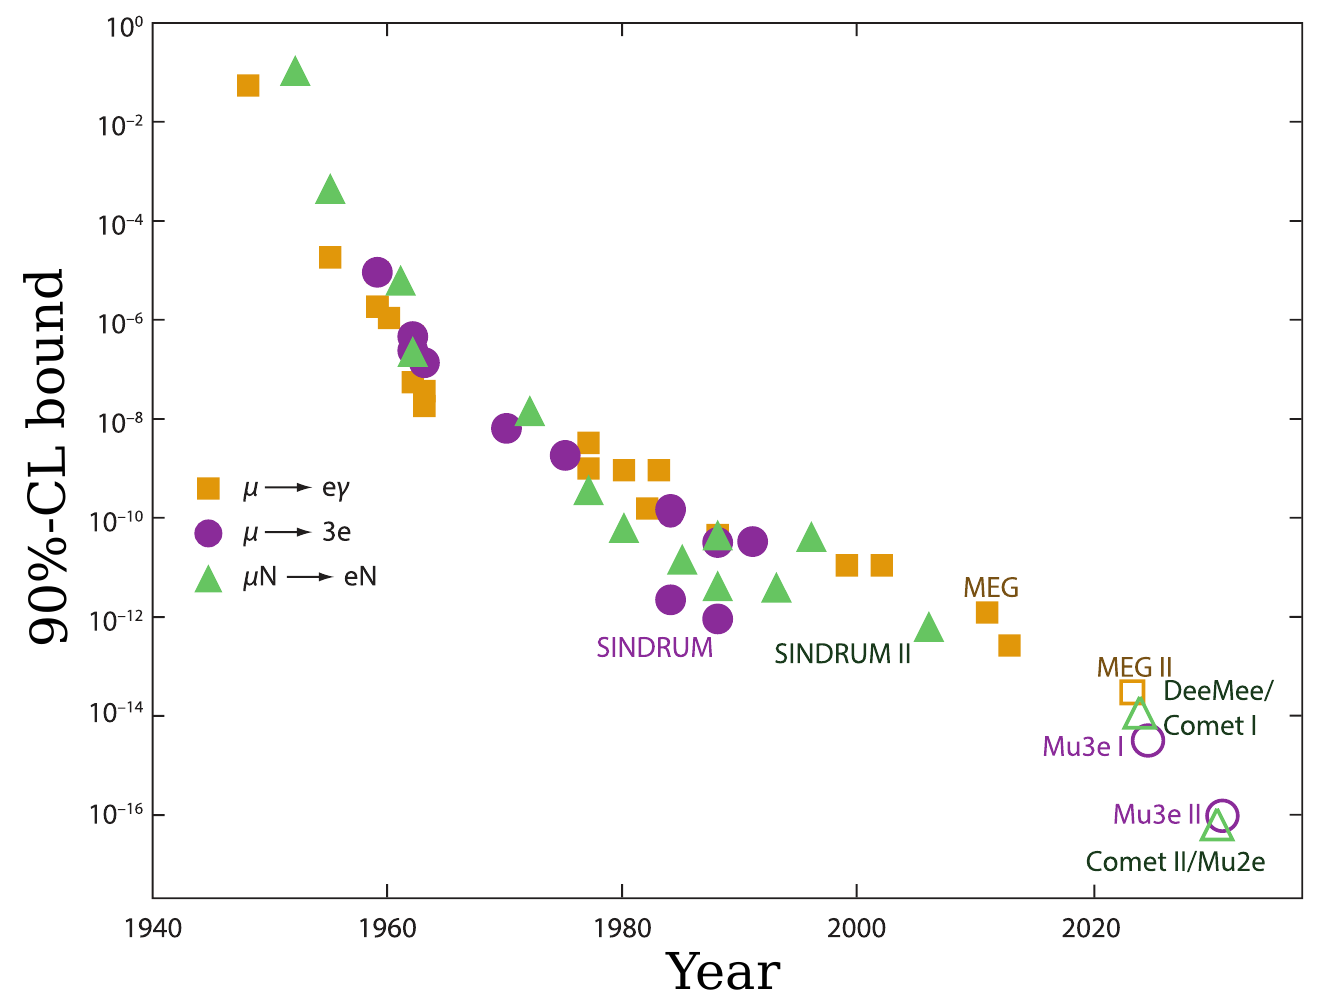
\includegraphics[width =0.7\textwidth]{figures/png/Screenshot_20240307_161549.png}
\caption{History and outlook of branching ratio limits in muon rare decay modes, Ref. \cite{MARCIANO1977303}.}
\label{fig:muchannel}
\end{figure}
\begin{figure}[!h]
\centering
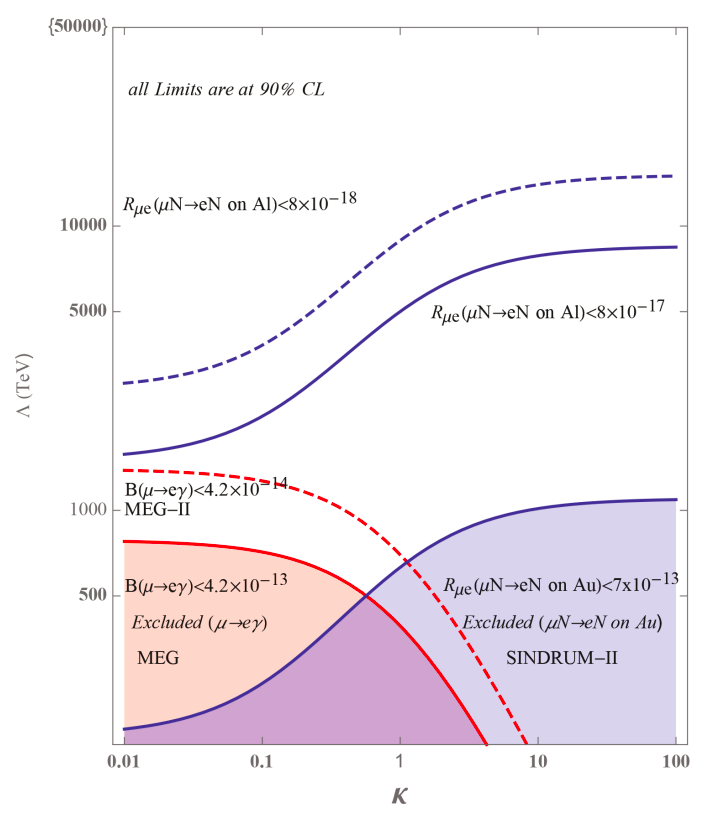
\includegraphics[width =0.7\textwidth]{figures/png/Screenshot_20240313_120457.png}
\caption{Sensitivity of $\mu \rightarrow e\gamma$ and $\mu N \rightarrow eN$ experiments to the new physics
scale $\Gamma$ as a function of $\kappa$ as defined in Equation \ref{LCF}, Ref. \cite{CGroup:2022tli}. The blue region is the New
Physics phase space excluded by SINDRUM-II, Ref. \cite{SINDRUMII:2006dvw}. The red region represents the
limit set by MEG, Ref. \cite{megi}, while the dashed red line represents the region that is
excluded by MEG-II, Ref. \cite{megiicollaboration2024search}. The solid (dashed) blu line is the
expected limit that would be set by Mu2e, Ref. \cite{universe9010054}.}
\label{fig:muchannelbr}
\end{figure}
\subsubsection{$\mu^+ \rightarrow e^+ \gamma$}
A clear signal of CLFV, in $\mu^+ \rightarrow e^+ \gamma$ channel, is given by back-to-back electron and photon, each one with energy of 52.8 MeV, 
both produced simultaneously. Positive muons are preferred since the negative ones may undergo the nuclear capture. 
Muons are stopped and decay at rest. There are two most significant sources of background: Radiative Muon Decay (RMD) $\mu^+ \rightarrow e^+ \nu_e \bar{\nu}_\mu \gamma$ 
and the accidental coincidence of $\mu^+ \rightarrow e^+ \nu_e \bar{\nu}_\mu$ with a random $\gamma$ 
generated by annihilation or bremsstrahlung. The first one is an in-time process, where neutrinos carry off a small part of the energy 
and it is only a small part of the total background. The accidental background is dominant. Since both backgrounds scale with the muon stop rate $\Gamma_\mu$, a continuous beam is preferred. 
Moreover, since an higher number of stopped muons correspond to a lower statistical error, but at the same time to a lower signal to background ratio, an optimal $\Gamma_\mu$ exists.
The stopping target thickness must optimized: a thin target is needed to minimise Multiple Coulomb Scattering, which affects the angular resolution of the outgoing electron, but 
it must be thick enough to block a significant portion of incoming muons. 
\paragraph{The MEG Experiment}
The MEG experiment, Ref. \cite{megi}, has been designed around two concepts: exploiting a liquid
xenon detector (LXe) for positron and photon tracking and an anti-bottle magnetic field, Ref. \cite{clfv_signorelli}. 
The apparatus is shown in Figure \ref{fig:meg}. A polyethylene target is used to stop muons in the center of the magnet. 
The measured quantities are the electron and photon energies ($E_e$ and $E_\gamma$) and the
relative positions (angles $\theta_{e\gamma}$, $\phi_{e\gamma}$ and time $t_{e \gamma}$).
A combination of drift chambers (DCH) and plastic scintillator timing counters (TC) measures the positron momentum.
The photon energy and direction are measured in a volume of LXe with more than 800 photo-multipliers tubes. 
An energy resolution of less than 1\% for each particles is required to distinguish background from the signal. 
In MEG, the magnetic field decreases uniformly from centre to periphery, pushing particles away from the centre. 
The exact shape of the field has been chosen to have a track radius proportional to the absolute momentum.
This allows low energy positrons to be discarded by simply placing the detector far enough away from the magnet axis. 
This feature is unique to the MEG magnetic system and justifies its name as \textit{COnstant Bending RAdius} (COBRA) magnets.
The DCH spectrometer is composed by 16 trapezoidal drift chambers oriented radially and filled with He-C$_2$H$_6$. 
The timing from the DCH and TC is used to assess the radial coordinate, whereas the $z$ location is determined by measuring the induced
charged on the zig-zag shaped pads on the side of the drift chambers. The momentum resolution for $e^+$ is $\sim$ 330 keV.
A liquid xenon scintillating detector was used for photon reconstruction to reduce passive material and improve temporal resolution. 
This option provides more light yield than NaI crystals and has a substantially shorter decay period, with photon interaction times measured at less than 100 ps.
MEG collected $7.5 \times 10^{14}$ stopped muons in 2008-2013, setting a limit of $BR(\mu^+ \rightarrow e^+ \gamma) < 4.2 \times 10^{-13}$ at 90\% C.L., Ref. \cite{megi}.
\begin{figure}[!h]
\centering
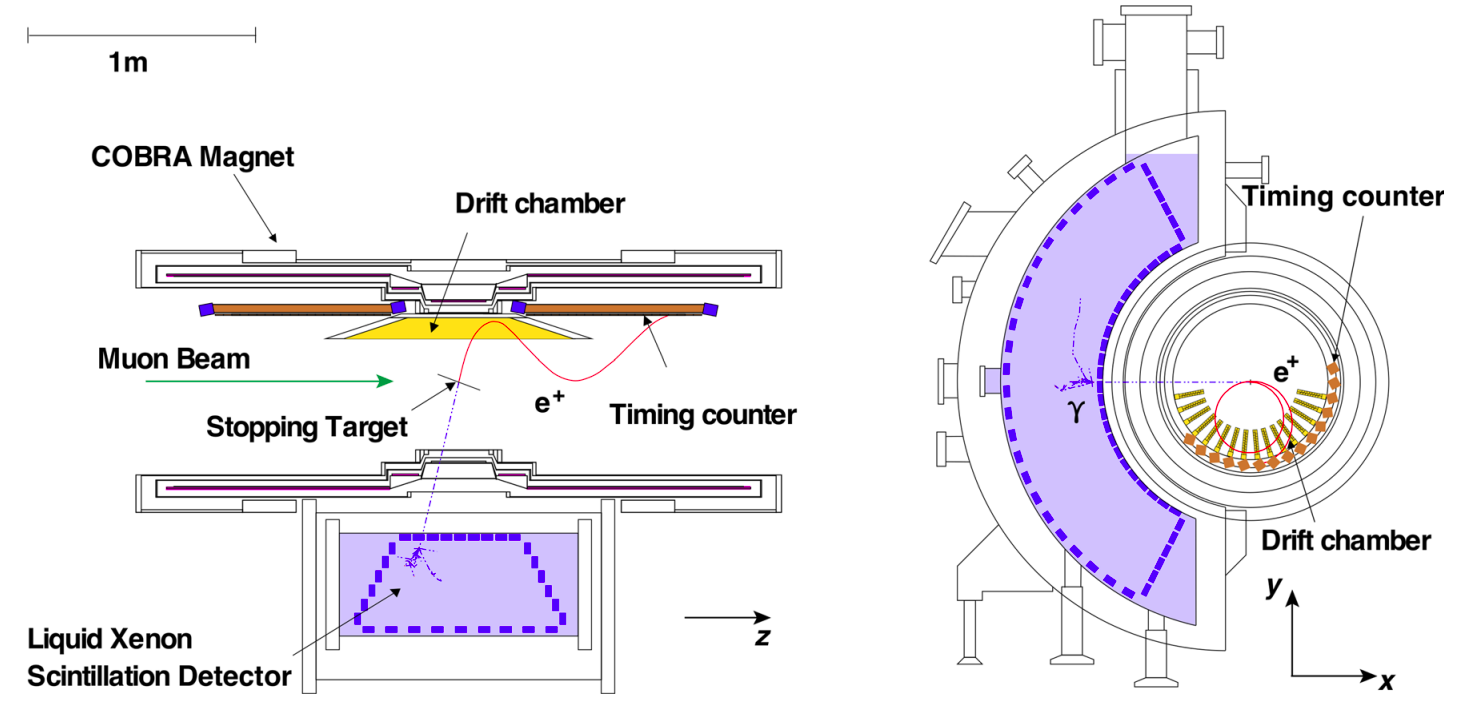
\includegraphics[width =0.8\textwidth]{figures/png/Screenshot_20240321_115127.png}
\caption{Schematic view of the MEG detector, Ref. \cite{megi}.}
\label{fig:meg}
\end{figure}
\paragraph{The MEG II experiment}
The MEG II detector is the upgrade to the MEG one, Ref. \cite{megiicollaboration2024operation}.
MEG II was proposed to reduce the contamination due to the accidental background that could not be further reduced in MEG.
In Figure \ref{fig:meg2}, the apparatus is shown. The muon flux was increased up to $7 \times 10^7 \ \mu^+$/s and a thinner but more inclined 
stopping target was installed to reduce the multiple scattering and bremsstrahlung 
while keeping the same stopping power (205 $\rightarrow$ 140 $\mu$m).
The old drift chamber was replaced with a new cylindrical drift chamber (CDCH) designed
to have higher granularity and transparency and made of 9 layers of drift cells to
improve positron track reconstruction. CDCH is shown in Figure \ref{fig:meg2}.
A more segmented system (pixellated-TC) was adopted instead of plastic scintillator timing counters (TC).
A Radiative Decay Counter was introduced, that is a target of scintillator and LYSO calorimeter positioned transversely to detect positron from RMD emitted at low angle.
When combined with the final result of MEG, MEG II collaboration obtained the most stringent limit up to date, $BR(\mu^+ \rightarrow e^+ \gamma)<3.1\times 10^{-13}$ 90\% C.L., Ref. \cite{megiicollaboration2024search}.
The MEG II collaboration took data in 2022 and 2023, collecting much more statistics compared to 2021. By 2026, more than twenty-fold increase in statistics is foreseen, with the goal of reaching a
$BR(\mu^+ \rightarrow e^+ \gamma)\lesssim 6\times 10^{-14}$ 90\% C.L..
\begin{figure}[!h]
    \centering
    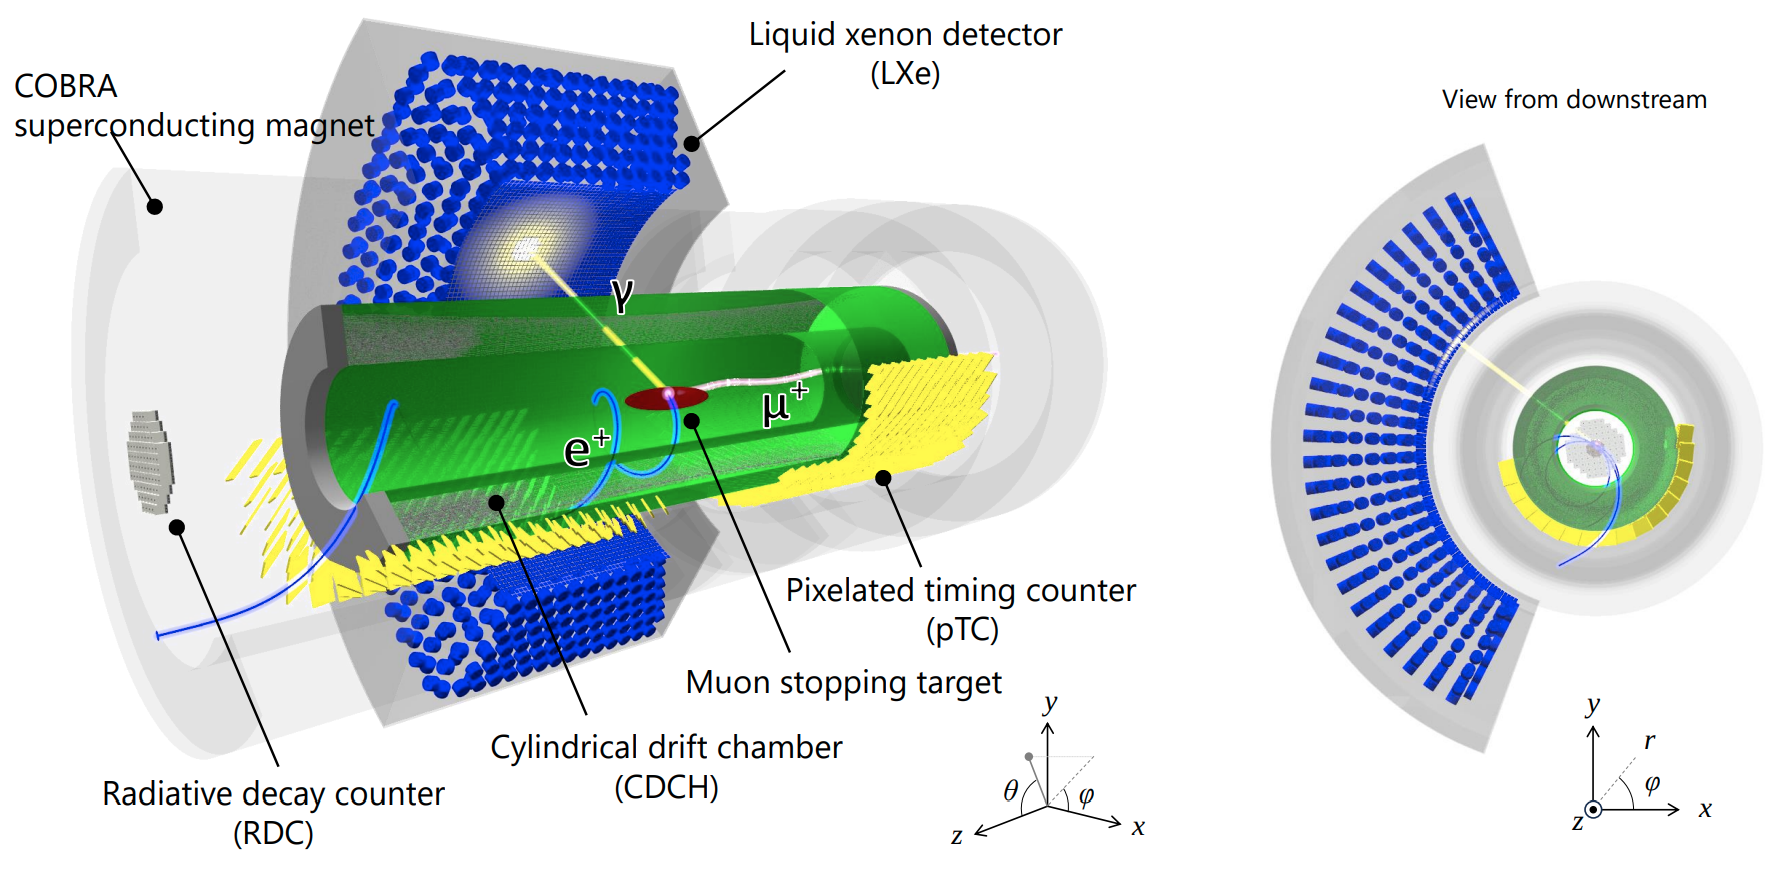
\includegraphics[width =0.8\textwidth]{figures/png/Screenshot_20240307_140116.png}
    \caption{A sketch of the MEG II detector with a simulated $\mu^+ \rightarrow e^+ \gamma $ event, Ref. \cite{megiicollaboration2024operation}.}
    \label{fig:meg22}
    \end{figure}
\begin{figure}[!h]
\centering
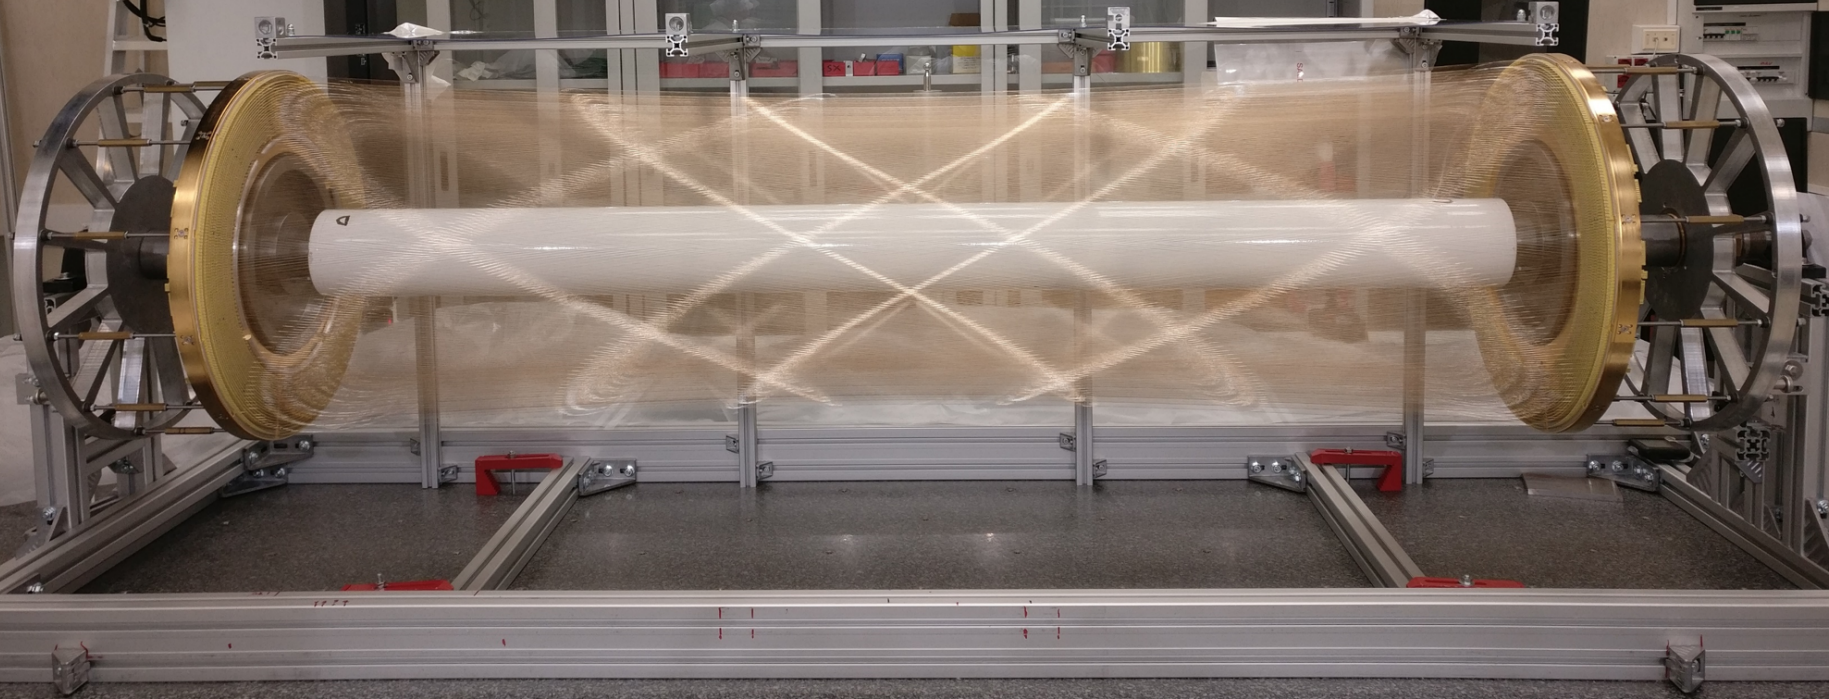
\includegraphics[width =0.8\textwidth]{figures/png/Screenshot_20240307_140235.png}
\caption{Picture of the open CDCH equipped with all the wires, Ref. \cite{megiicollaboration2024operation}.}
\label{fig:meg2}
\end{figure}






\subsubsection{$\mu^+ \rightarrow e^+ e^-  e^+ $}
The CLFV signature of the $\mu^+$ decay at rest consists of two $e^+$ and one $e^-$ at the same time, 
with total energy equal to the muon mass and null vector sum of the
particle momenta.  The exact energy distribution of daughter particles needs understanding of the underlying physics, 
which is currently unknown. To establish detector efficiency, the fraction of particles with momentum over a certain 
threshold requires some physical assumptions.
There are two main sources of background. The first one is the radiative muon decay with 
internal conversion, $\mu^+ \rightarrow e^+ \gamma \nu_e \bar{\nu}_\mu$ with the radiative
photon internally converting into an electron pair $\mu^+ \rightarrow e^+ e^+ e^- \nu_e \bar{\nu}_\mu$. 
This process has a branching ratio of $BR\sim 3.4 \times 10^{-5}$.
An experimental resolution of $\sim$1 MeV is needed in order to be sensitive to the small energy carried off by the neutrinos. 
The second source of background is due to the coincidence of one Michel decay with a $e^+e^-$ pair (1-MD) or two Michel decays with a single $e^-$ (2-MD). 
In this case, the $e^+e^-$ pair can be produced by Bhabha scattering or photon conversion, while the $e^+$
can be produced by Compton scattering or mis-reconstructed $e^+$ and $e^+e^-$ (with the $e^-$ not reconstructed). 
As a consequence, this source of background depends on the muon rate and
can be suppressed with precise vertex reconstruction, timing and track reconstruction.
As in the previous channel, the use of a continuous beam is preferred.
Since this is a three-body decay and particles momenta span a range between few MeV 
and half the muon mass, a thin and low-mass tracker with an excellent resolution is needed. 
\paragraph{SINDRUM I}
The current best limit on $\mu^+ \rightarrow e^- e^+ e^+$, $1.0 \times 10^{- 12}$ at 90\% C.L., was set by the
SINDRUM I experiment at PSI, Ref. \cite{sindrumi}. A schematic view of the SINDRUM spectrometer is given in Figure \ref{fig:sindrumi}. 
The spectrometer consisted of a double cone-shaped stopping target in the middle of five concentric multi-wire proportional chambers surrounded by an array of plastic
scintillator counters inside a solenoidal magnetic field. Considering a 50 MeV $e^-/e^+$, the detector 
apparatus had a momentum resolution at the level of $\sim$1 MeV, a timing
resolution $\leq$1 ns and a vertex resolution of $\sim$1 cm. The trigger consisted of a charge filter, requiring one negative and two positive particles, within a time window of 7 ns, Ref. \cite{universe8060299}.
\begin{figure}[!h]
\centering
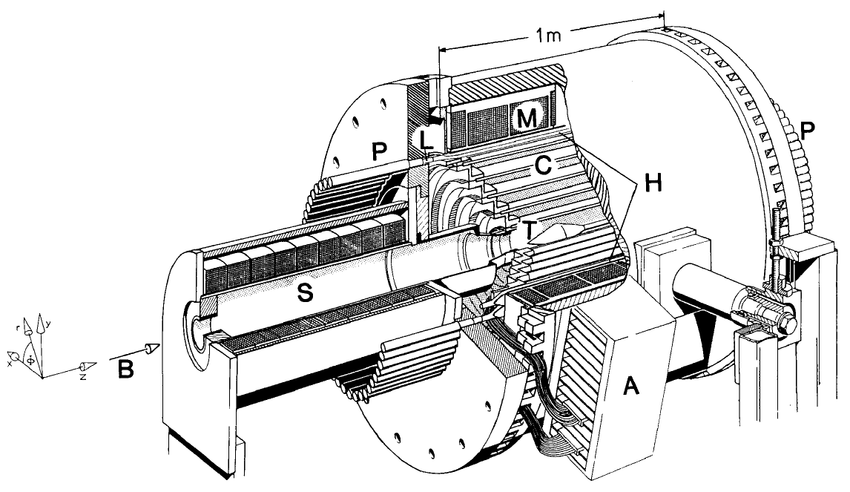
\includegraphics[width =0.8\textwidth]{figures/png/The-SINDRUM-I-detector-in-the-horizontal-operating-orientation.png}
\caption{Schematic view of the SINDRUM experiment, Ref. \cite{sindrumi}.}
\label{fig:sindrumi}
\end{figure}

\paragraph{The Mu3e Experiment}
The goal of the Mu3e experiment is to achieve a single-event-sensitivity of the order
of $10^{-16}$ on the $\mu^+ \rightarrow e^+ e^-  e^+ $ decay, Ref. \cite{hesketh2022mu3e} and \cite{papa}. 
A schematic view of Mu3e is shown in Figure \ref{fig:mu3e}.
The same muon beam as MEG II experiment will employed, stopping muons on a thin hollow double-come Mylar target. 
A 2 m cylinder will be placed inside a 1.5 T magnetic field and segmented in 5 sections. 
The central station will consist of two double layers of pixel detectors and a
scintillating fiber tracker. The other four stations will be made of two layers of pixel
sensors and a hodoscope of scintillator. Since the Mu3e search relies heavily on accurate track reconstruction, multiple Coulomb
scattering is a limiting factor and the technical choices adopted for the detector design
have been taken to minimize this effect. The tracker consists of High Voltage Monolithic
Active Pixel (HV-MAPS) and the design is such as to exploit the (partial) canceling of
the multiple scattering in half of turn. The estimated time and vertex resolutions are
$\sigma_t \sim 100$ ps and $\sigma_{xy} \sim 200 \ \mu$m and the momentum resolution will be 100 $\div$ 400 keV for 10 $\div$ 53
MeV particles. The experiment is projected in three phases. During the first one, the beam will have an intensity of $\mathcal{O}(10^7) \ \mu^+$/s 
and there will be only the tracker installed. After that, the beam with an intensity of $\mathcal{O}(10^8) \ \mu^+$/s will 
be used and the scintillating fibers and two of the additional tracking stations will be added.
During the third phase, beam intensity will increase up to $\mathcal{O}(10^9) \ \mu^+$/s and to 
reach the single-event-sensitivity of $10^{-16}$, two stations will be added.
\begin{figure}[!h]
\centering
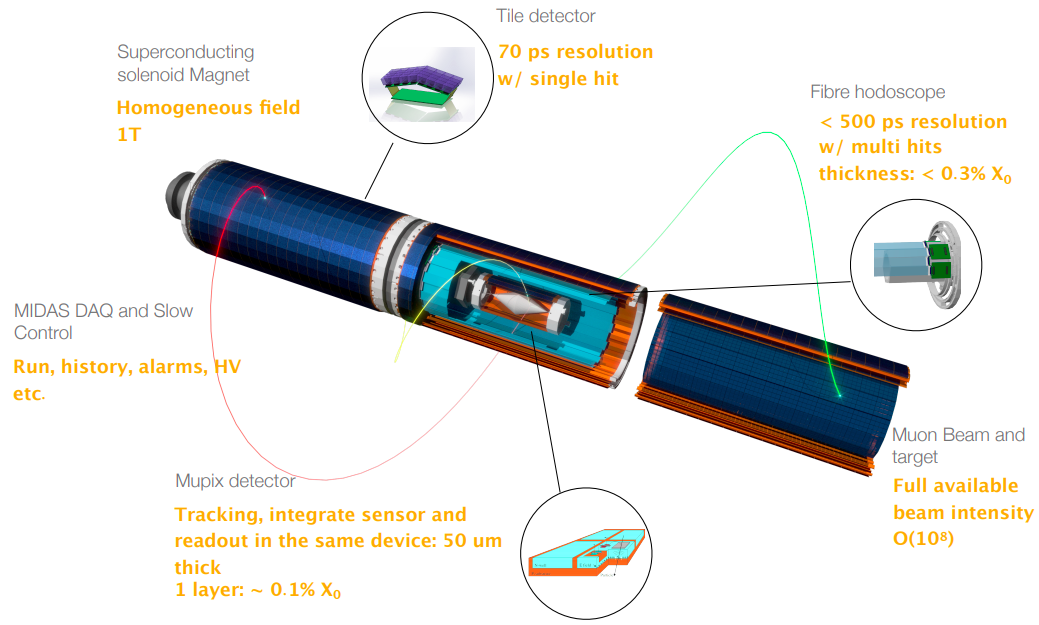
\includegraphics[width =0.8\textwidth]{figures/png/Screenshot_20240321_143650}
\caption{Mu3e experimental setup layout (3D view). An example of a $\mu^+ \rightarrow e^+ e^-  e^+ $ decay event is shown, Ref. \cite{papa}.}
\label{fig:mu3e}
\end{figure}









\subsubsection{$\mu^- N \rightarrow e^- N $}
In this CLFV channel, negative muons are captured by a nucleus and the decay products are detected. The coherent conversion leaves the nucleus
intact and minimal energy will be transmitted to the nucleus recoil.
The signal signature is a monochromatic 105 MeV $e^-$. All other 105 MeV signals may be a source of background. 
Cosmic rays can generate or can be misidentified as electrons in the signal region.
Decay in orbit (DIO) can contaminate the signal region and High energy photons produced by radiative captures of pions (RPC) and muons (RMC) can convert 
asymmetrically and generate high energy electrons. More detailed discussion about signal and backgrounds will be given in Section \ref{sigandbkg}.
Among the previous processes, this channel offers the most powerful sensitivity. 
Thanks to the one particle final state, this channel is not affected by accidental background.
Another advantage, with respect to the $\mu \rightarrow e \gamma$ search, is the larger momentum
and better separation of the electron signal from the background. The background level, due to low-momentum particles, can be reduced
thanks to the \textit{hollow-cylinder} detectors. The muon capture process is incredibly fast ($\mathcal{O}(10^{-13})$ s) and is characterized by the emission of
an X-ray, that can be detected. To cancel the uncertainty due to the overlap of the nucleus and the muon wave
functions, the commonly used quantity to denote results in this type of searches is:
\begin{equation}
    R_{\mu e}=\frac{N(\mu \rightarrow e)}{N(\text{muon capture})}
\end{equation}
Through the detection of X-ray from muon capture, the denominator can be easily determined.
A pulsed beam is preferred as discussed in Section \ref{sigandbkg}.
A characteristic of these experiments is that the apparatus lends itself to the additional
search of the process $\mu^- N \rightarrow e^+ N$ which would violate also the leptonic number.
\paragraph{SINDRUM II}
PSI delivered a 1 MW 590 MeV proton beam that was extracted from the ring
cyclotron and directed onto a 40 mm carbon target. The beam line
transported secondary particles ($\pi$, $\mu$, $e$) emitted in the backward direction to the SINDRUM II spectrometer, as
illustrated in Figure \ref{fig:sindrumii}. The structure of the experiment
was cylindrical. The gold target (B), which had a radius of 20 mm, was positioned
in the middle of the cylinder. Two drift chambers (F and G) were adopted to measure
the helical trajectories, with the ionization electrons drifting radially towards the amplification 
regions. The tracker used CO$_2$-isobutane (70\%/30\%) as a drift
gas while the second one He-isobutane (85\%/15\%). Two 3 mm thick plastic scintillator hodoscopes (D) and a 3 cm 
thick plexiglass Cherenkov hodoscope (E) provided trigger and time information. 
The device included two end-cap hodoscopes at opposite ends of the tracking zone to aid in triggering 
and resolving ambiguities during event reconstruction.The number of muons stopped
was monitored observing the characteristic muonic gold X-rays passing through the
superconducting coil of the spectrometer. A Ge(Li) detector was used for this purpose.
SINDRUM II set the limit on the muon conversion at $7 \times 10^{-13}$, Ref. \cite{SINDRUMII:2006dvw}.
\begin{figure}[!h]
\centering
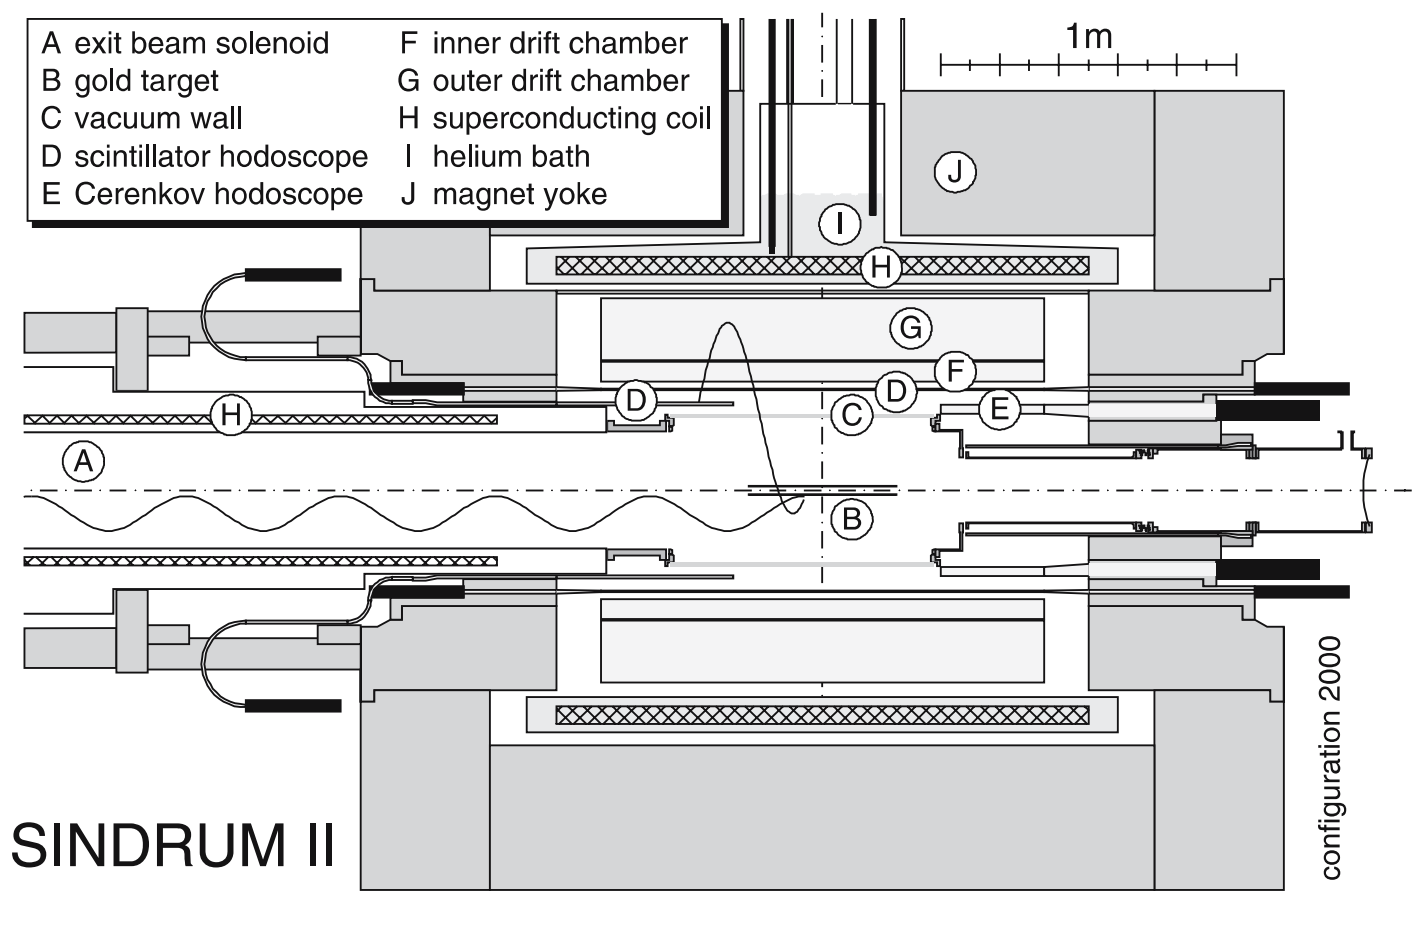
\includegraphics[width =0.8\textwidth]{figures/png/Screenshot_20240307_163120.png}
\caption{Pictorial view of the SINDRUM II experiment, Ref. \cite{SINDRUMII:2006dvw}.}
\label{fig:sindrumii}
\end{figure}
\paragraph{Mu2e}
Mu2e will employ an 8 GeV, 25 kW pulsed proton beam, with 100 ns wide bunches spaced by 1.7 $\mu$s. 
Figure \ref{fig:mu2escheme} shows a schematic view of the experimental setup and of the
three sections of the experiment: Production Solenoid, Transport
Solenoid and Detector Solenoid. The $S$ shape lowers the background due to 
neutral particles and selects the charge sign: almost only negative muons will hit the stopping target. 
The straw tube tracker and the crystal electromagnetic calorimeter are located down-stream of the Al target. 
Both these detectors adopted a \textit{hollow-cylinder} geometry. 
The estimated Mu2e sensitivity after three years of data taking is $R_{\mu e} < 3 \times 10^{-17}$, Ref. \cite{universe9010054}.
Mu2e will be described extensively in the Chapter \ref{mu2echapter}.
The Mu2e Collaboration is also performing preliminary studies for the upgraded Mu2e II, Ref. \cite{dukes}. 
The proton beam intensity will be improved by the PIP-II upgrade that will increase the rate of stopped muons 
on target from $10^{10} \ \mu^-$/s to $10^{11} \ \mu^-$/s. New detector technologies are under study for the upgraded
Mu2e II.
\paragraph{COMET}
The COherent Muon-to-Electron Transition (COMET) experiment is under construction at
the Japanese Proton Accelerator Research Center (J-PARC), Ref. \cite{Abramishvili_2020}. 
This experiment shares several characteristics with Mu2e. COMET will employ a 8 GeV, 56 kW pulsed proton beam
with 1.17 $\mu$s spaced bunches. The two main differences between
COMET and Mu2e can be seen from the schematic view of these experiments in Figure \ref{fig:comet}.
Using a C-shaped transport solenoid instead of an S-shaped a more precise muon momentum selection 
is possible, but there will be a lower beam intensity of $\sim$70\%.
An additional curved solenoid after the stopping target filters out non 
interesting electrons before they reach the tracker.
COMET will be developed in two stages: Phase-I and Phase-II. The two-step strategy is motivated by uncertainties of physical processes. 
\subparagraph*{Phase-I} The first phase involves understanding experimental techniques and studying backgrounds, 
with an intermediate measurement of $R_{\mu e} \sim 7\times 10^{-15}$. The proton power will be restricted to 
3.2 kW and a single 90° bend will be employed. The major challenge is the short distance between all the elements. 
To track electrons, a cylindrical drift chamber will be used. To trigger and time the tracker, 
scintillating hodoscopes will surround the tracker. 
\subparagraph*{Phase-II} A straw tube tracker and a LYSO crystal electromagnetic 
calorimeter will be adopted to deal with the increased particle rate. 
The entire magnetic system will be  expanded.
After Phase-I, some physical processes will be better understood.
For example, the backward production by 8 GeV proton is now poorly known and the data on muon nuclear
capture in aluminum are still quite scarce. 
\begin{figure}[!h]
\centering
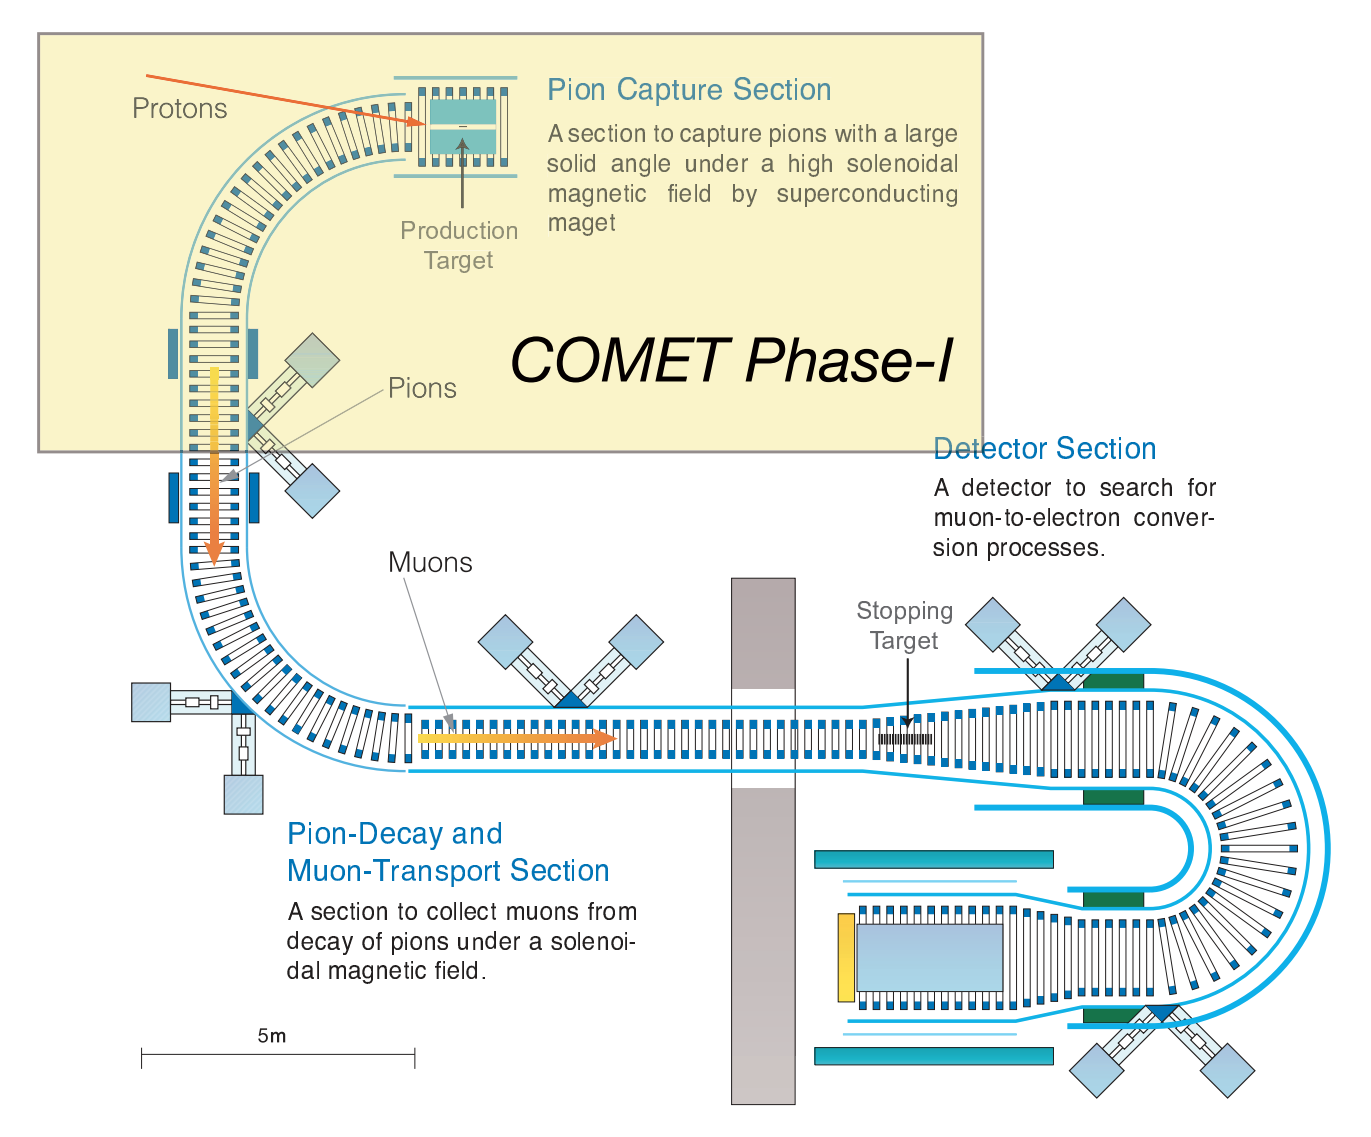
\includegraphics[width =0.7\textwidth]{figures/png/Screenshot_20240307_152133.png}
\caption{Conceptual view of the staging approach in COMET experiment, Ref. \cite{Abramishvili_2020}.}
\label{fig:comet}
\end{figure}
\paragraph{DeeMe}
A simpler setup will be adopted by the Direct emission of electron from Muon to electron conversion (DeeMe) 
experiment at J-PARC to search the muon-to-electron conversion, Ref. \cite{deeme}.
A pictorial view of DeeMe experiment is shown in Figure \ref{fig:deeme}.
The experiment will use the Muon Science Establishment's new beam-line (H-line), 
which will provide 3 GeV protons (a pair of bunches separated by 600 ns at 25 Hz) 
that will hit on the production target. Some muons ($\mathcal{O}(10^{10})\mu$/s) will be stopped in the target itself, 
allowing for a search for $\mu \rightarrow e$ with just one target. The signal will be detected 
with multi-wire proportional chambers and a spectrometer. 
A dipole will remove low momentum background particles from the transport system. 
The experiment aims to achieve a single-event sensitivity of $10^{-13}$ using a graphite target, 
followed by $10^{-14} \div 10^{-15}$ (depending on running duration) using a silicon carbide (SiC) target with a higher capture rate. 
\begin{figure}[!h]
    \centering
    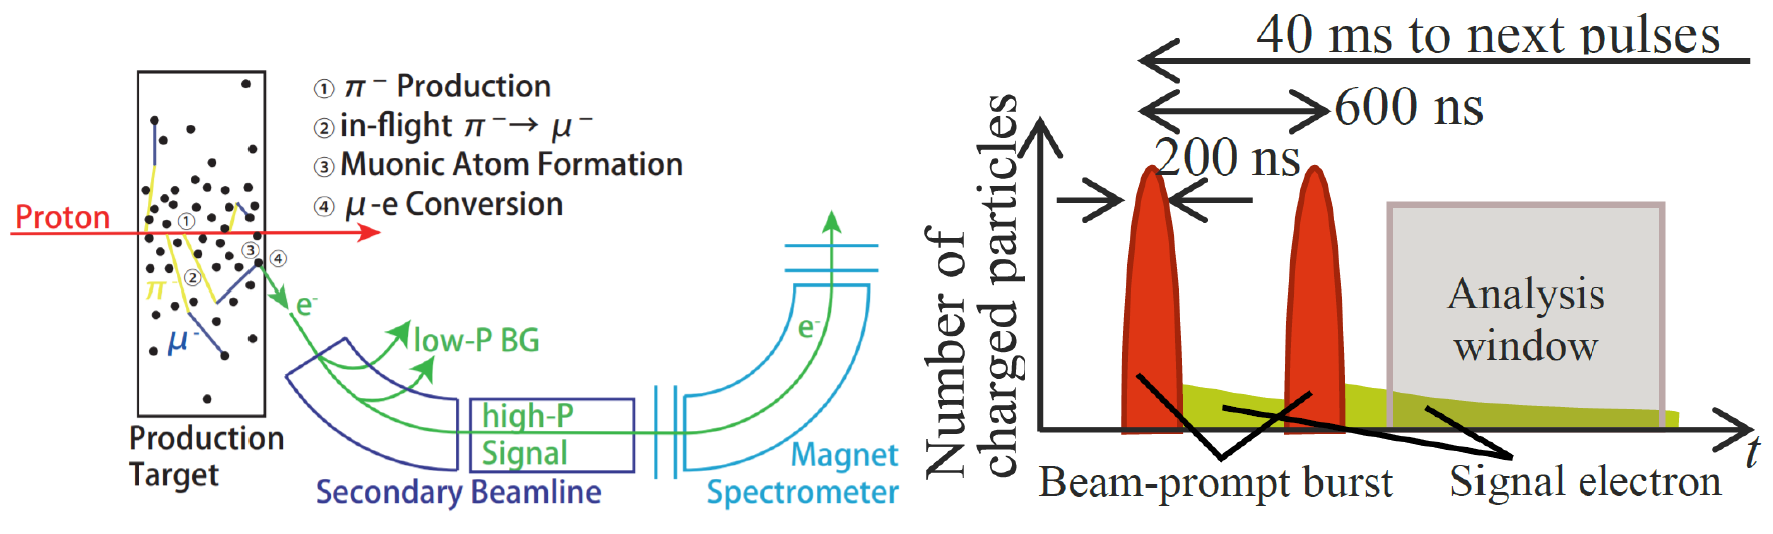
\includegraphics[width =0.8\textwidth]{figures/png/Screenshot_20240322_101840.png}
    \caption{Schematic view and timing structure of the DeeMe experiment, Ref. \cite{deeme}.}
    \label{fig:deeme}
    \end{figure}
\subsection{$\tau$ Channels}
The $\tau$ lepton is a very promising source of CLFV decays, Ref. \cite{universe8060299}. 
The huge $\tau$ mass ($m_\tau$ $\sim$ 1.777 GeV) allows for the investigation of multiple CLFV channels, in comparison with muon decays, Ref. \cite{clfv_signorelli}: 
$\tau^\pm \rightarrow l^\pm \gamma$, $\tau \rightarrow 3l$ and $\tau\rightarrow l \ h$, 
where $h$ is a light hadron and $l$ is an electron or muon. The $\tau$ sector of a CLFV search takes advantage from an higher predicted branching ratio, compared to muons, 
according to $(\frac{m_\tau}{m_\mu})^\alpha$, where $\alpha$ depends on the model. Table \ref{tab:upperlimits} lists the current best limits on the $\tau$ 
CLFV searches and Figure \ref{fig:tauchannel} displays the results from the BaBar, Ref. \cite{PhysRevD.77.091104}, Belle, Ref. \cite{ABASHIAN2002117} and LHCb, 
Ref. \cite{TheLHCbCollaboration2008}. The $\tau$ particle has a short lifetime ($\tau_\tau \ \sim$ 2.91 $\times$ 10$^{-13}$ s), with respect to the muon.
As a result, it is not possible to produce $\tau$ beams and strong electron or proton accelerators are required to produce $\tau$s with a large generation cross section. 
To constrain the kinematics of decay, large detectors with good particle identification, tracking, calorimetry, and hermeticity are required. 
Because $\tau$ CLFV searches are done with beams and detectors used for a broader physics programme, 
the increased sensitivity derived by its greater mass is partially decreased by the number of $\tau$s that can be detected.
In these experiments, a pair of $\tau^+ \tau^-$ is produced by the decay of $\Upsilon(4s)$ resonance at $\sqrt{s}=10.58$ GeV. The branching ratio of this process is  $90\%$ of 
the one of $b \bar{b}$. One $\tau$ decays via Standard Model (SM) process (tag side), while the signal side is determined based on the specific topology of each channel. 
At $e^+ e^-$ and $pp$ colliders, the $\tau$s are not created at rest. Because of the boost, the decay products could have 
energy of several GeV, posing an experimental challenge of providing wide-range calibrations for detectors (from a few hundred MeV to several GeV), Ref. \cite{universe8060299}.
In a short time, the Belle 2 experiment at Super KEKB will try to increase its limits below $5 \times 10^{-9}$ or $10^{-9}$ for the radiative and three body decays respectively, 
with an integrated luminosity of 50 ab$^{-1}$. The main background, in $\tau \rightarrow l \gamma$ channel only, arises from
$e^+ e^- \rightarrow \mu^+ \mu^- \gamma$ or $e^+ e^- \rightarrow \tau^+ \tau^- \gamma$ where one of the $\tau$s decays via $\tau \rightarrow \nu \bar{\nu}$.
To reduce the background, it is possible to use the $\tau$ polarization or to collect large samples of
$\tau$ leptons at a lower center-of-mass energy, where initial state radiation is negligible in the signal region. This might be the situation in a $\tau$-charm 
factory operating slightly above the $\tau$ production threshold, Ref. \cite{Bennett_2016}.
\begin{figure}[!h]
\centering
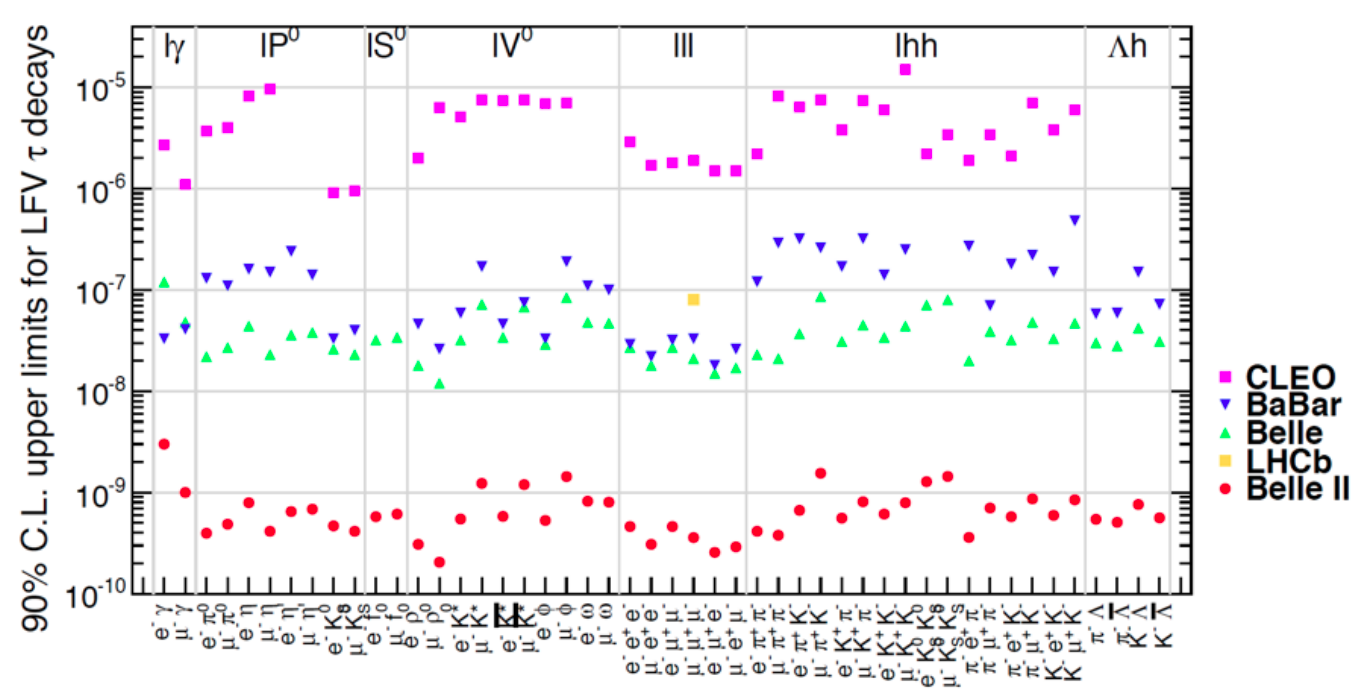
\includegraphics[width =0.7\textwidth]{figures/png/Screenshot_20240319_134052.png}
\caption{Tau lepton-flavor-violating branching ratio 90\% C.L. upper limits summary plot, Ref. \cite{universe4100101}. The green and blue cones 
are respectively the Belle and Babar's best upper limits. The red dots are Belle II's expected upper limits for the 50 ab$^{-1}$ run.}
\label{fig:tauchannel}
\end{figure}

\iffalse
\subsection{$K$ and other Mesons Channels}
There are several CLFV processes that involve $K$ mesons:
\begin{itemize}
    \item Axial Vector and Pseudoscaler: $K^0_L \rightarrow \mu^\pm e^\mp $ and $K^0_L \rightarrow \pi^0 \mu^\pm e^\mp$;
    \item Vector and Scalar: $K^+ \rightarrow \pi^+ \mu^+ e^-$ and $K^+ \rightarrow \pi^+ \mu^- e^+$;
    \item Total lepton number violating: $K^+ \rightarrow \pi^- \mu^+ e^+$.
\end{itemize} 
Kaons have many more decay modes than muons so many more potential sources of background. They also
come with lots of either neutrons and gammas or charged pions.


\begin{figure}[!h]
\centering
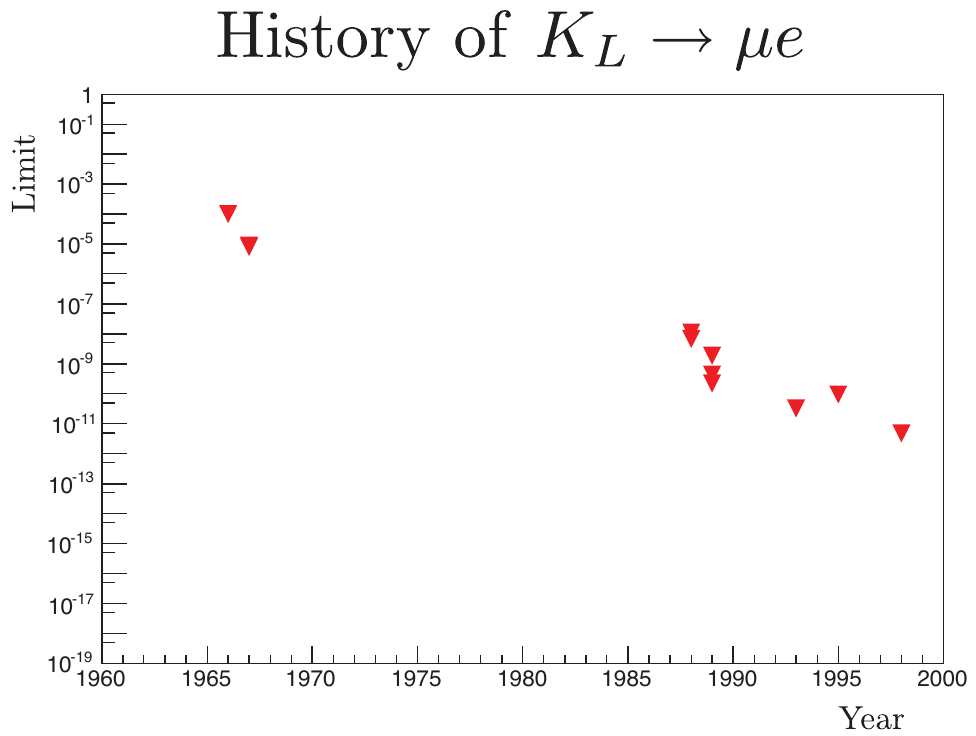
\includegraphics[width =0.4\textwidth]{figures/png/Screenshot_20240307_114258.png}
\caption{.}
\label{fig:Kchannel}
\end{figure}

\fi

\chapter{The Mu2e Experiment}\label{mu2echapter}
\textit{
The Mu2e experiment aims to investigate the phenomenon of charged-lepton flavour 
violating (CLFV) neutrino-less conversion, where a negative muon transitions into 
an electron within the field of an aluminium nucleus. The experiment will use as variable for the results 
the ratio between the conversion and the nuclear muon capture rates:
\begin{equation}\label{rmue}
R_{\mu e}=\frac{\mu^{-}+N(Z, A) \rightarrow e^{-}+N(Z, A)}{\mu^{-}+N(Z, A) \rightarrow \nu_\mu+N(Z-1, A)}
\end{equation}
The goal is to improve the current limit, set by the SINDRUM-II experiment \cite{SINDRUMII:2006dvw}, by
four orders of magnitude and reach a SES (single-event-sensitivity) of 2.3 $\times$ 
10$^{-16}$ on the
conversion rate, a 90\% CL of 6.2 $\times$ 10$^{-16}$ and a 5$\sigma$ discovery 
reach at 1.2 $\times$ 10$^{-15}$ during Mu2e Run I.
Mu2e is presently undergoing commissioning and integration at the 
Fermilab Muon Campus, 
with contributions from an international collaboration. Data taking is planned to 
begin in 2026. 
This Chapter provides an overview of the Mu2e experimental techniques and infrastructure. 
Fundamental bibliography for this chapter can be found in \cite{bartoszek2015mu2e}, 
\cite{bobbb}, \cite{Bernstein_2013}, \cite{Kargiantoulakis_2020}, \cite{universe9010054}.}

\section{Experiment concept}
The Mu2e concept has been proposed back in 1989 by V. Lobashev and R. Dzhilkibaev \cite{lobachev}, 
and it relies on the following principles. 
A beam of negative muons, $\mu ^-$, is generated by directing a proton beam at a 
production target, yielding negative pions along with other mesons and hadrons. 
Pions, with a decay rate of more than 99.9\% due to helicity suppression, undergo 
$\pi ^- \rightarrow \mu ^- \bar{\nu}_\mu$ decay in flight. 

Low-momentum secondary muons are trapped by a Stopping Target (ST) to form muonic atoms. 
Within approximately $10^{-13}$ s, 
a muonic atom transitions to the $1s$ state \cite{MEASDAY2001243}. 
Given the brief cascading time compared to the mean muon lifetime in a muonic atom,  
instances of muon decay before reaching the ground state are negligible. 
The cascades emit photons, aiding in estimating the number of muons captured 
on the ST. 
Muonic atoms decay after a lifetime that depends on the ST material. 
In the Mu2e experiment, an Aluminum ST is adopted resulting in a lifetime of 
864 ns. Muons interacting with a nucleus mostly undergo two processes: 
nuclear capture $\mu^- N \rightarrow \nu_\mu N'^* $, where $N'^*$ represents an excited 
Magnesium nucleus, and muon decay-in-orbit (DIO), 
that is the three-body decay with neutrinos $\mu ^- N \rightarrow e^- N \nu_\mu \bar{\nu}_e$. 
As shown in Figure \ref{fig:muonicatom}, the ratio between these 
processes varies with the ST material. For $^{27}$Al, approximately 60.9\% 
of muonic atoms undergo muon nuclear capture. The remaining 39.1\% undergo muon DIO. 
The experiment aims to identify a third process, neutrinoless muon-to-electron 
conversion $\mu^- N \rightarrow e^- N $. Detectors will search for the signature of a 
single monochromatic electron.

The Mu2e experiment can also detect a lepton-number violation process 
$\mu^- N \rightarrow e^+ N'$.
This process violates both the charged lepton flavour and the total lepton number 
conservation ($|\Delta L|$ = 2). 
Conversion positrons tracks helices in the tracker, but with different chirality from electrons. 
\section{Signals and backgrounds}\label{sigandbkg}
\subsection{Conversion Electron signal}

The specific goal of Mu2e search is the neutrino-less coherent $\mu^- \rightarrow e^-$
conversion in the field of an aluminum nucleus: the electron recoils off the 
entire nucleus and follows two-body decay kinematics \cite{bartoszek2015mu2e}. The mass of the nucleus is large compared to the 
mass of the electron, hence the recoil terms are minimal. The outgoing nucleus 
remains in the ground state and as a result the signature of the process is a monochromatic conversion electron 
(CE) with the energy slightly lower than the muon's rest mass:
\begin{equation}
    E_{CE} = m_\mu - E_{recoil}(A) - E_{bind}(Z) 
\end{equation}
where $m_\mu$ is the muon mass, $E_{recoil}\simeq \frac{m^2_\mu}{2 m_N}$ is 
the recoil energy of the target nucleus, with $m_N$ the nucleus mass, and 
$E_{bind}\simeq \frac{Z^2 \alpha^2 m_\mu}{2}$ is the binding energy of the 
$1s$ state of the muonic atom \cite{universe9010054}. For the Mu2e 
ST material, $^{27}$Al, $E_{CE}$ = 104.97 MeV \cite{PhysRevD.84.013006}.
\subsection{Backgrounds}\label{backgrounds}
In order to improve the experimental sensitivity by four orders of magnitude 
it is important to know the experimental backgrounds. 
There are five categories of background 
sources \cite{bartoszek2015mu2e}:
\begin{enumerate}
\item electrons or muons coming from cosmic rays;
\item muon Decay-in-Orbit (DIO) and Radiative Muon Capture (RMC);
\item antiproton annihilation in the beamline and in the ST;
  \item radiative pion capture (RPC), decays in flight (DIF).
\end{enumerate}
  
The detailed discussion of these background sources will be provided below, along with the 
corresponding strategies to reduce  
them. 
\subsubsection{Cosmic rays}
Cosmic ray particles, predominantly muons, also contribute to the experiment 
background. Several processes that may occur are listed here:
\begin{enumerate}
    \item muon decays occurring within or near the detectors;
    \item muons interacting with nuclei within detectors or surrounding materials;
    \item muons scattering within the detectors and being erroneously identified as electrons.
    
\end{enumerate}

Detailed simulations estimated that in the Mu2e experiment, 
conversion-like signals generated by cosmic rays occur approximately once per day \cite{CRVposter}.

Mitigation involves making use of a combination of active veto and shielding.
The Mu2e Cosmic Ray Veto (CRV) system is described in Section \ref{CRV}.

\subsubsection{Intrinsic backgrounds}
The intrinsic backgrounds originate from two physics processes: 
muon decay-in-orbit (DIO) and radiative muon capture (RMC). In this context, 
$intrinsic$ denotes that this source of background is generated by the same muons
used to perform the conversion signal search. It consequently scales with the
stopped muon flux and the number of protons on target.


\paragraph{Muon Decay-in-Orbit}
Electrons energy coming from the three body decay of a free muon, 
$\mu^- \rightarrow e^- \bar{\nu}_e \nu_\mu$, is described by the Michel 
spectrum. The differential decay rate can be computed \cite{michel}:
\begin{equation}
    \frac{\text{d}\Gamma_{\text{free}}}{\text{d}x}= \frac{G^2_F m^5_\mu}{192 \pi^3}x^2(6-4x+\frac{\alpha}{x}f(x)) 
\end{equation}
where $x=\frac{2 E_e}{m_\mu}$, $0\leq x\leq 1$, $G_F$ is the Fermi constant, 
$\alpha$ is the fine-structure constant, $m_\mu$ is the muon mass, $E_e$ is the 
electron energy and $f (x)$ represents a complicated radiative correction term, 
described in \cite{PhysRev.113.1652}.

However, the presence of an Al nucleus allows the electron to 
interact with it, exchanging momentum and resulting in a maximum possible energy, called 
$endpoint$ $energy$, being the same as the CE energy. 
As shown in Figure \ref{fig:linearscalemichel}, the spectrum (with the presence of the Al nucleus) peaks at 
52.8 MeV, which is the half of the muon rest energy or the energy of the searched CE.
The difference between the two energy spectra, one neglecting the nuclear recoil and the 
other one in the presence of the Al nucleus, is illustrated in Figure \ref{fig:micheldiff}. 
Figure \ref{fig:logscalemichel} shows a more detailed zoom on the high-energy 
range of the spectrum. When the electron energy $E_e \ \geq$ 85 MeV, the dominant term 
at the leading order scales with $(E_{\mu e} - E_e)^5$ \cite{PhysRevD.84.013006}, 
resulting in a low rate within the energy range very close to the endpoint. However, due to 
the energy loss of particles interacting with ST or detector materials and radiative corrections, 
the CEs tend to be reconstructed with a left-skewed energy distribution,
with a full width at half maximum (FWHM) approximately on the order of 1 MeV 
\cite{gaponenko}, as shown in Figure \ref{fig:sensitivity}.

A particle tracking detector with high momentum resolution 
also helps to reduce background, which will be explored in the next sections.



\begin{figure}[!h]
     \begin{subfigure}[b]{0.4\linewidth}
         \centering
         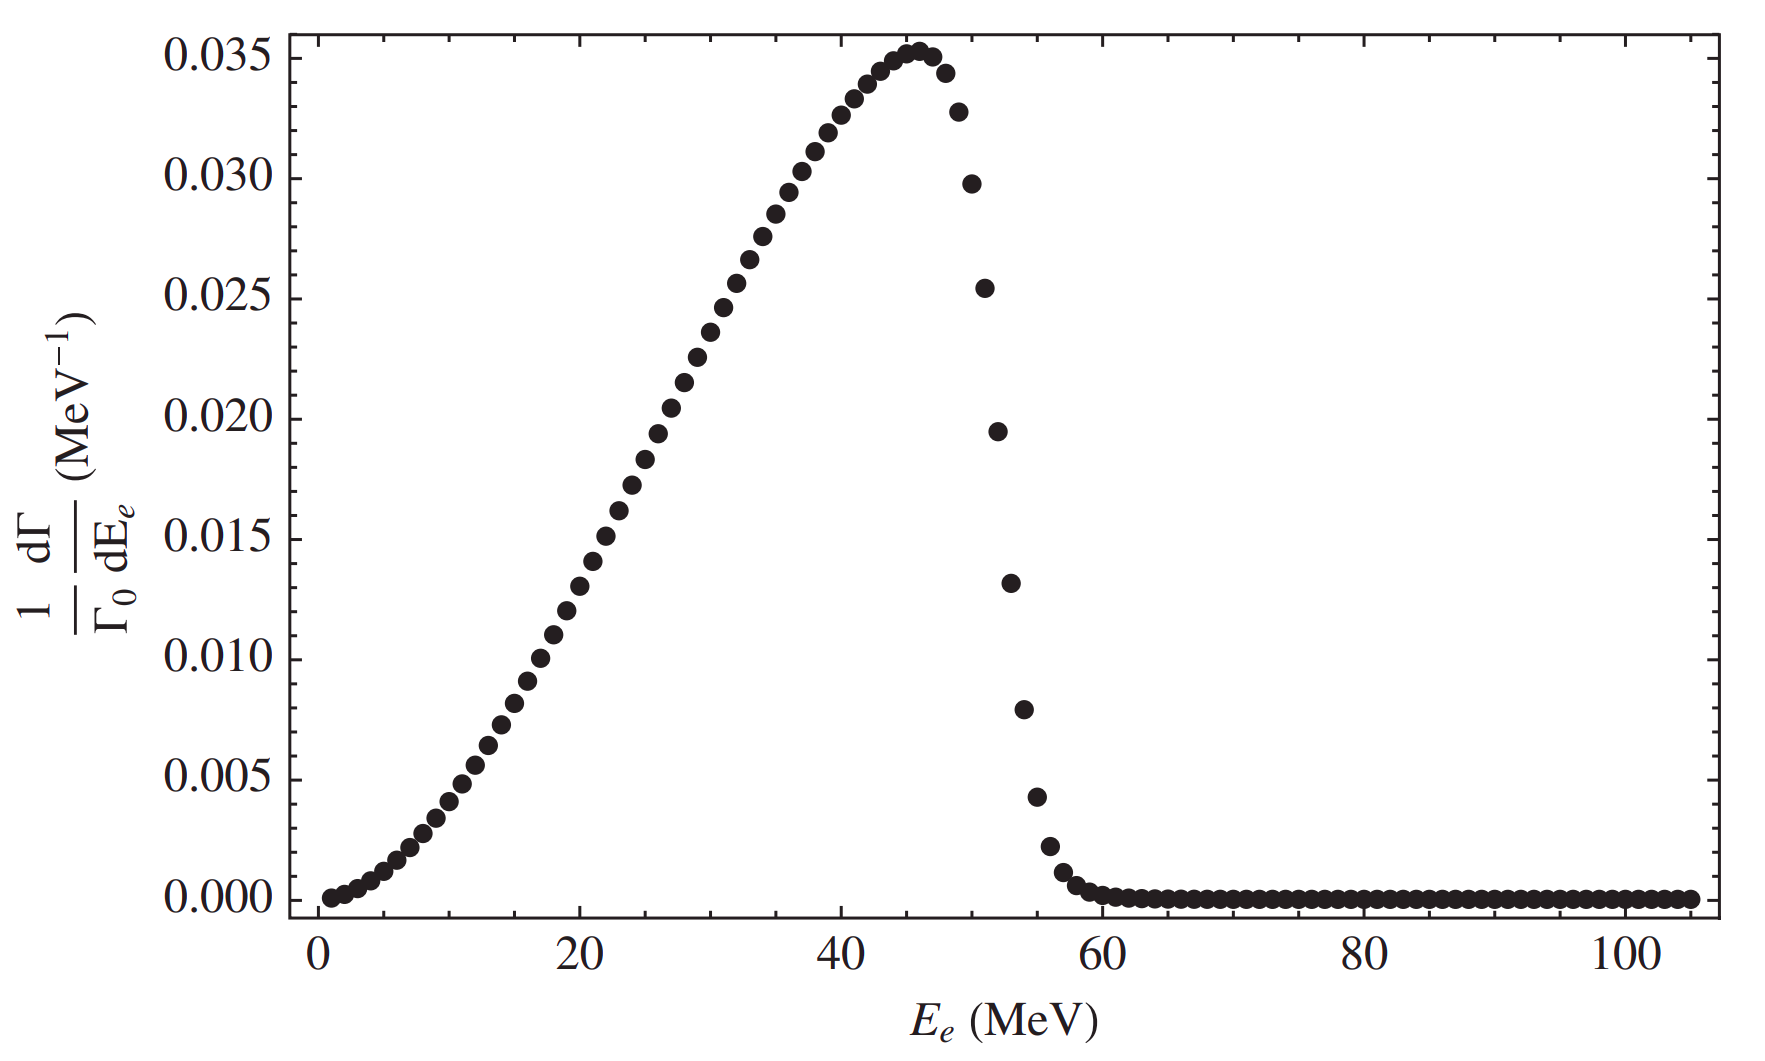
\includegraphics[scale = 0.18]{figures/png/Screenshot_20240222_175415.png}
         \subcaption{Linear scale.}
         \label{fig:linearscalemichel}
     \end{subfigure}
     \begin{subfigure}[b]{0.7\linewidth}
         \centering
         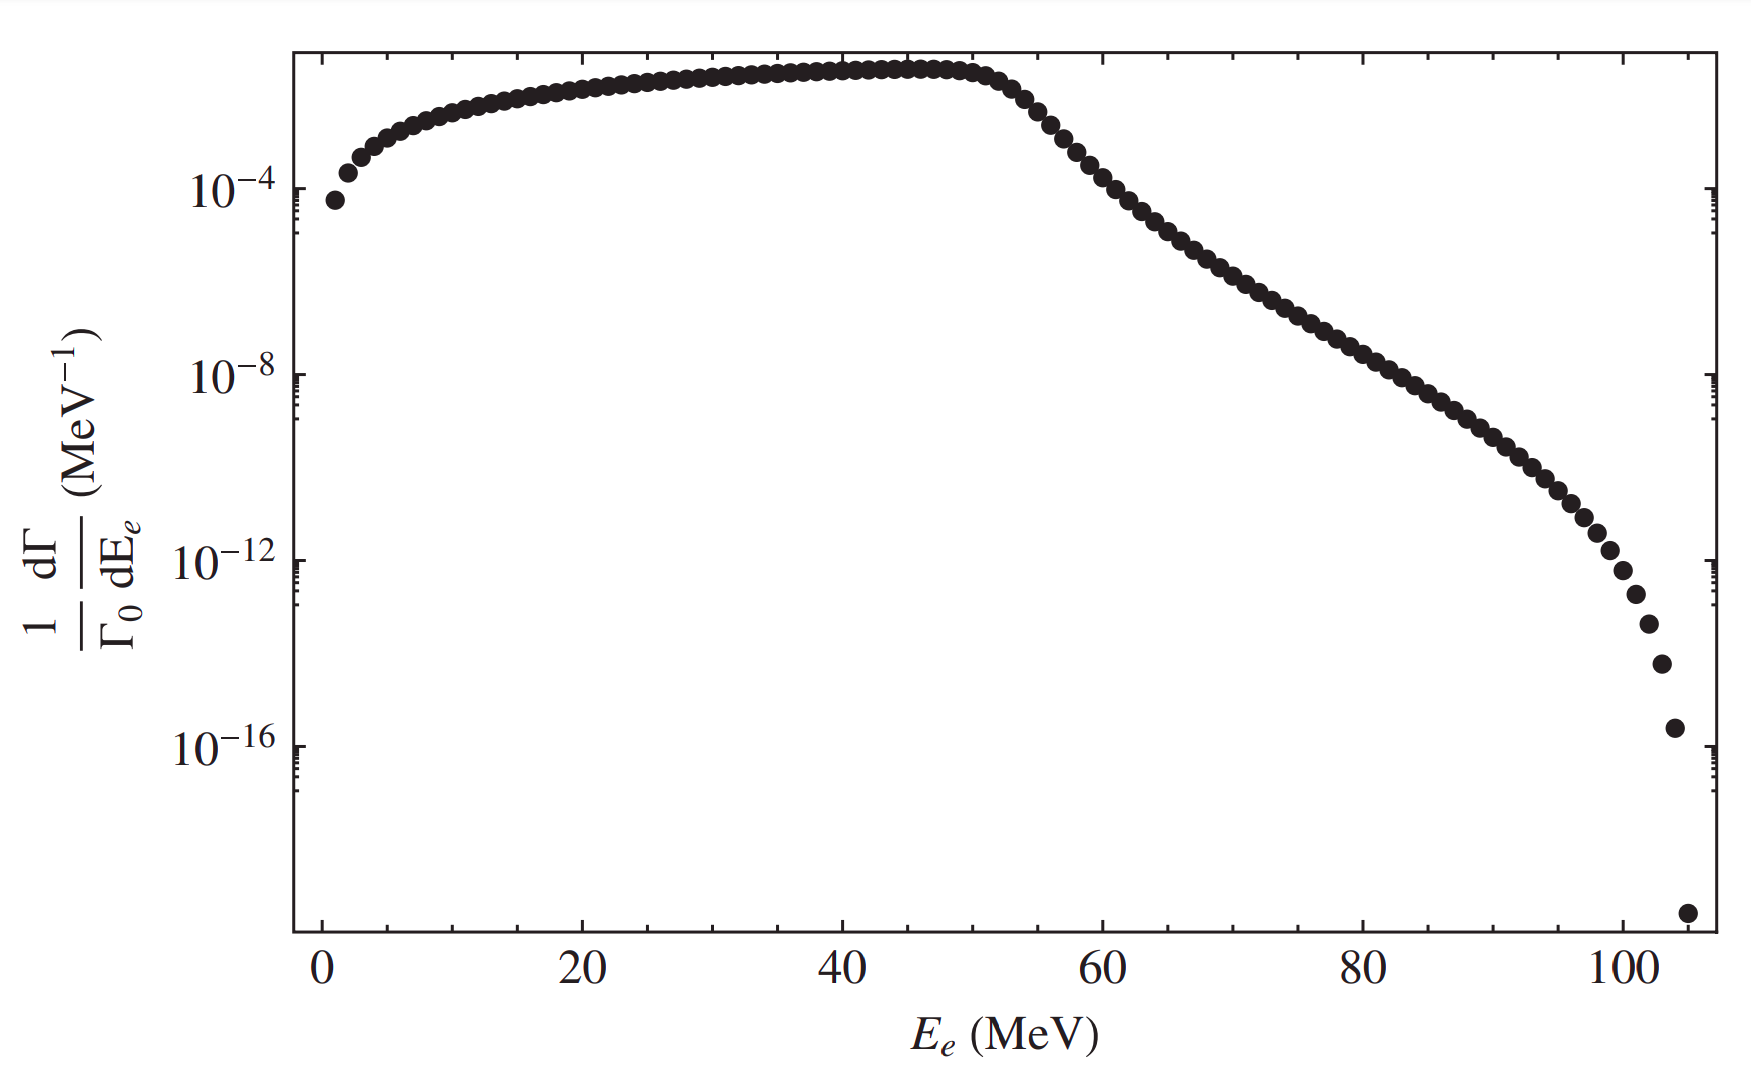
\includegraphics[scale = 0.18]{figures/png/Screenshot_20240222_175446.png}
         \subcaption{Logarithmic scale.}
         \label{fig:logscalemichel}
     \end{subfigure}
     \caption[Decay-in-orbit spectrum on aluminium.]{
       Decay-in-orbit electron spectrum on Al \cite{PhysRevD.84.013006}.}
        \label{fig:michel}
\end{figure}

\begin{figure}[!h]
\centering
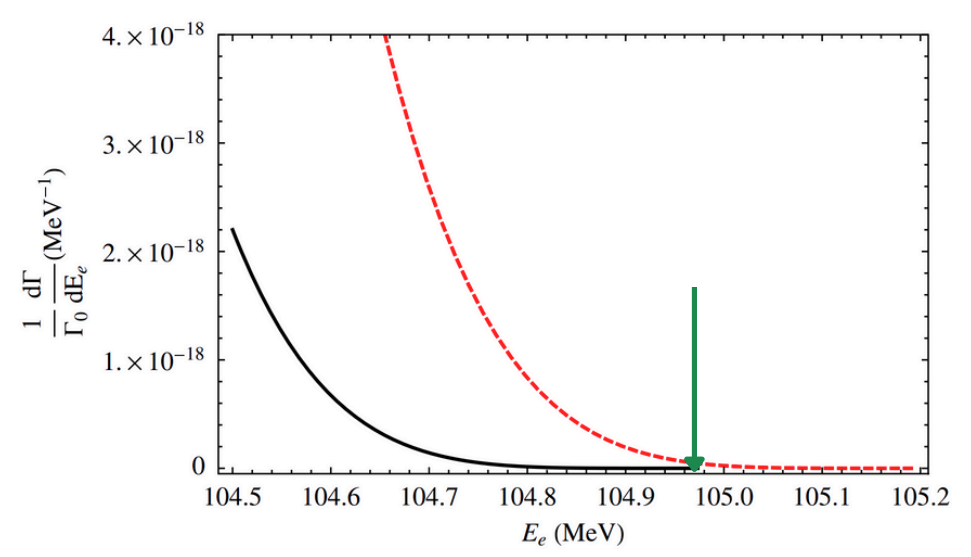
\includegraphics[width =0.55\textwidth]{figures/png/Screenshot_20240909_141143.png}
\caption[The electron energy spectrum near to the endpoint.]{The electron energy spectrum near to the endpoint. The black line 
represents the Michel spectrum w/o the nuclear recoil, while the red 
dashed line takes into consideration the recoil of the Al nucleus 
\cite{PhysRevD.84.013006}. The green arrow shows the spectrum end at 104.973 MeV.
}
\label{fig:micheldiff}
\end{figure}


\paragraph{Radiative Muon Capture}
The Radiative Muon Capture (RMC) is a muon capture with emission of an energetic photon.

In the process $\mu^- N \rightarrow\gamma \nu_\mu N'^* $, 
the photon can either be real or virtual. The photon, interacting with matter or 
undergoing pair production, can produce electrons with energies close to $E_{CE}$, 
introducing background to the experiment. The emitted photon's energy follows 
a spectrum, with its maximum energy, denoted as the kinematic limit $k_{max}$, 
determined by the equation \cite{bartoszek2015mu2e}:

\begin{equation}
k_{max} = m_\mu c^2 - |E_b| - E_{rec} - \Delta M ,
\end{equation}

where $E_b$ represents the muon binding energy on the initial nucleus, $E_{rec}$  
the recoil energy of the daughter nucleus and $\Delta M$ is the rest energy difference 
between the final and initial nuclei. This formula neglects higher order nuclear effects. 
RMC can be effectively mitigated in the Mu2e experiment by 
selecting Al as the ST material. The ST is selected so that the daughter nuclide of a muon-capture 
process of any kind is heavier than the original nuclide. For aluminum, the RMC photon 
endpoint energy is 101.9 MeV, approximately 3.1 MeV below the CE energy 
\cite{bartoszek2015mu2e}. 
The FWHM of the conversion peak is around 1 MeV, therefore the RMC background will be 
outside the signal region. However, the RMC background might distort the DIO spectra 
around 100 MeV range, making it difficult to extrapolate the high momentum end of the DIO spectrum. 
The RMC background will be determined from the positron data.


\subsubsection{Prompt processes}
This type of background sources can generate electrons at roughly the same time as 
the entering beam particles. There are four primary sources: radiative pion capture (RPC), 
pion decay-in-flight ($\pi$-DIF), muon decay-in-flight ($\mu$-DIF) and beam electrons.

\paragraph{Radiative Pion Capture}

Pions, reaching the ST and captured in Al can 
produce high-energy photons, i.e. $\pi^- N(A,Z) \rightarrow \gamma N ^* (A,Z-1)$. 
This process, called radiative pion capture,
has a branching ratio of $\sim 2\%$ \cite{PhysRevC.5.1867}.
Similar to RMC, the photon 
can internally convert into an electron-positron pair or be radiated as an on-shell photon 
and convert in the detector material producing an $e^+e^-$ pair. 
The resulting electrons contribute to the experiment background. 
Despite its similarity to RMC, RPC is a more challenging background to suppress due to 
the fact that the endpoint of the energy spectrum of photons, and consequently the 
resulting electrons, is not constrained by the rest energy of the muon.
The pion mass is 139.6 MeV, above the CE energy,
and the spectrum of the electrons resulting from RPC overlaps with the search region. 
The SINDRUM II results 
were limited by the pion-induced background and also by the low intensity of its muon 
beam \cite{SINDRUMII:2006dvw}. SINDRUM II used a primary proton beam with a 
frequency of one pulse every 19.75 ns, lasting approximately 0.3 ns. This interval 
between pulses was shorter than the 26 ns lifetime of pions \cite{zyla}, 
ensuring a consistent pion flux. To mitigate RPC, SINDRUM II made use of a degrader to suppress 
pions and a veto counter in the beam, resulting in less than one out of 10$^9$ pions reaching their 
target. However, given the more intense beam, the Mu2e experiment has to change the approach. 
Mu2e will suppress the RPC background by delaying the search window in time with respect
  to the incoming beam by several hundred nanoseconds \cite{universe9010054}. 
One important point to note is that the out-of-time protons could produce $late$ pions not rejected by the delayed timing window. 
Consequently, it is important for the pulsed beam to achieve a high extinction level. Further elaboration 
on the pulsed beam used in Mu2e will be provided in Section \ref{accel}.
\paragraph{$\pi$-DIF and $\mu$-DIF}
The pion decay-in-flight ($\pi$-DIF) and the muon decay-in-flight ($\mu$-DIF) 
exhibit quite similar characteristics. Free pions and muons can 
undergo electron decay while transitioning from the 
production target to the ST, through the processes 
$\mu^- \rightarrow e^- \nu_\mu \bar{\nu}_e$ and 
$\pi^- \rightarrow e^- \bar{\nu}_e$. In the center-of-mass 
frame of the initial particles, electrons originating 
from the first process exhibit an energy spectrum that 
reaches an endpoint of 52.8 MeV, while those from the 
second process have a consistent energy of approximately 
70 MeV. Since the pions and muons move at relativistic velocities, 
the energies (and momenta) of the resultant electrons are 
boosted. For instance, a muon with a momentum of around 
79 MeV/c or a pion with momentum close to 70 MeV/c can generate 
an electron with an energy of 105 MeV \cite{bartoszek2015mu2e}. 
Implementing a pulsed proton beam and using a delayed 
live window can help suppress background from $\pi$-DIF and 
$\mu$-DIF events. Particles with sufficient momentum 
to boost the daughter electrons to the concerning energies 
move quickly along the muon beamline and are gone by the 
time the live search window begins \cite{bobbb}. 


\paragraph{Beam electrons}\label{beamelectrons}
Other mechanisms generate electrons, both at the production target 
and along the muon beamline. For instance, neutral pions formed at 
the production target can decay in two photons, after which the 
photons can either create electron-pairs or interact with nearby 
materials to generate electrons. 
The beam electron background is suppressed by the delayed search timing window.


\subsubsection{Delayed processes from antiprotons}
Protons, at a given threshold, can generate antiprotons 
within the production target. This occurs through the 
process of antiproton production: $pp \rightarrow ppp\bar{p}$. 
If we consider that all four particles in the final state are 
at rest in the center of mass frame, the minimum kinetic energy 
needed for $p\bar{p}$ production can be found, which is 
approximately $6 m_pc^2 \sim 5.6$ GeV, where $m_p$ is the 
mass of the proton. In an ideal scenario, maintaining the 
beam energy below this threshold could enable us to avoid 
this background in the experiment. Unfortunately, the Mu2e 
proton beam goes beyond the threshold for antiproton production. 
The antiprotons are long-lived and massive. Antiprotons with 
momenta below 100 MeV/c travel at speeds less than 0.1$c$, 
requiring several $\mu$s to spiral from the production target 
to the ST \cite{bartoszek2015mu2e}. They have the correct 
charge and momentum to pass through the collimators placed 
between the production target and the ST. Annihilating or 
undergoing interactions with other materials, they have the 
capability to release a substantial amount of energy, generating 
numerous electrons. The delayed timing of 
such interactions is much longer than the muon lifetime, leading to a 
continuous flow of antiprotons reaching the ST. The pulsed beam and 
the delayed live window fail to suppress the antiproton background. 
The best approach is to prevent the antiprotons from reaching the 
region where the ST is located.
Two thin absorbers are positioned in 
the muon beamline to capture the antiprotons. Their design was 
developed to find a compromise between increasing antiproton 
absorption and decreasing muon beam loss. 

\subsection{Background estimates and signal sensitivity}
Mu2e run plan is divided in two different phases. Run I 
will take place in 2027, before a 2 years shutdown due to the 
planned accelerator upgrade for the long baseline neutrino 
program. In Run I phase one, a low intensity proton beam, 
$1.6 \times 10^7$ protons/pulse, will be used. In Run I 
phase two, the mean intensity will be increased up to $3.9 \times 10^7$ 
protons/pulse. As discussed in \cite{universe9010054}, during Run I, the 5$\sigma$ discovery sensitivity is 
$R_{\mu e}^{5 \sigma} = 1.2 \times 10^{-15}$, with a 
total expected background of 0.11$\pm$0.03 events. 
Reaching the 5$\sigma$ significance level requires 
observing 5 $\mu\rightarrow e$ events in the two-dimensional search window 
103.60 < $p$ < 104.90 MeV/c, 640 < $T_0$ < 1650 ns. In the 
absence of a signal, the expected upper limit is $R_{\mu e}$<$6.2 \times 10^{-16}$
at 90\% CL. 
The single event sensitivity (SES) is defined as
\begin{equation}
    SES \equiv \frac{1}{N_{POT} \cdot P_{\mu \ stop} \cdot \epsilon_{CE} \cdot BR_{capture}}
\end{equation} 
where $N_{POT}$ is the number of protons on target in the experiment, 
$P_{\mu \ stop}$ is the number of muons stopped on target per 
proton, $\epsilon_{CE}$ is the CE acceptance, which is a product 
of detector efficiency (dependent on the momentum signal region) 
and fraction of muons interacting in the live time window and 
$BR_{capture}$ is the branching ratio of muon captures, which 
is 60.9\%. The optimized Mu2e signal window corresponds to a 
SES of $2.3 \times 10^{-16}$. The background estimates after 
the sensitivity optimization are summarized in Table \ref{tab:summarybkg}.

Figure \ref{fig:sensitivity} shows the momentum and time distributions 
for CE signal and background processes corresponding to the optimized 
signal window for Run I. A detailed analysis and an estimate of the Mu2e 
expected backgrounds for Run I can be found in \cite{universe9010054}.
\begin{center}  
\begin{table}[!h]
\centering
\renewcommand{\arraystretch}{1.2}
\begin{tabular}{| c | c |}
\hline
\textbf{Channel} & \textbf{Mu2e Run I}\\
\hline
SES & 2.4 $\times \ 10^{-16}$ \\
\hline
Cosmic rays & 0.046 $\pm$ 0.010 (stat.) $\pm$ 0.009 (syst.) \\
DIO & 0.038 $\pm$ 0.002 (stat.) $ ^{+ \ 0.025} _{- \ 0.015}$ (syst.)\\
Antiprotons & 0.010 $\pm$ 0.003 (stat.) $\pm$ 0.010 (syst.) \\
RPC in-time & 0.010 $\pm$ 0.002 (stat.) $ ^{+ \ 0.001} _{- \ 0.003}$ (syst.)\\
RPC out-of-time & (1.2 $\pm$ 0.1  (stat.) $ ^{+ \ 0.1} _{- \ 0.3}$ (syst.)) $\times$ $10^{-3}$ \\
RMC & $<$ 2.4 $\times$ $10^{-3}$ \\
Decays in flight & $<$ 2 $\times$ $10^{-3}$ \\
Beam electrons & $<$ 1 $\times$ $10^{-3}$ \\
\hline
Total &  0.105 $\pm$ 0.032\\
\hline
\end{tabular}
\caption{Summary of the several background sources to 
the CE search as expected in Mu2e Run I \cite{universe9010054}. 
The Table also shows the corresponding SES. }

\label{tab:summarybkg}
\end{table}
\end{center}
\begin{figure}[!h]
\centering
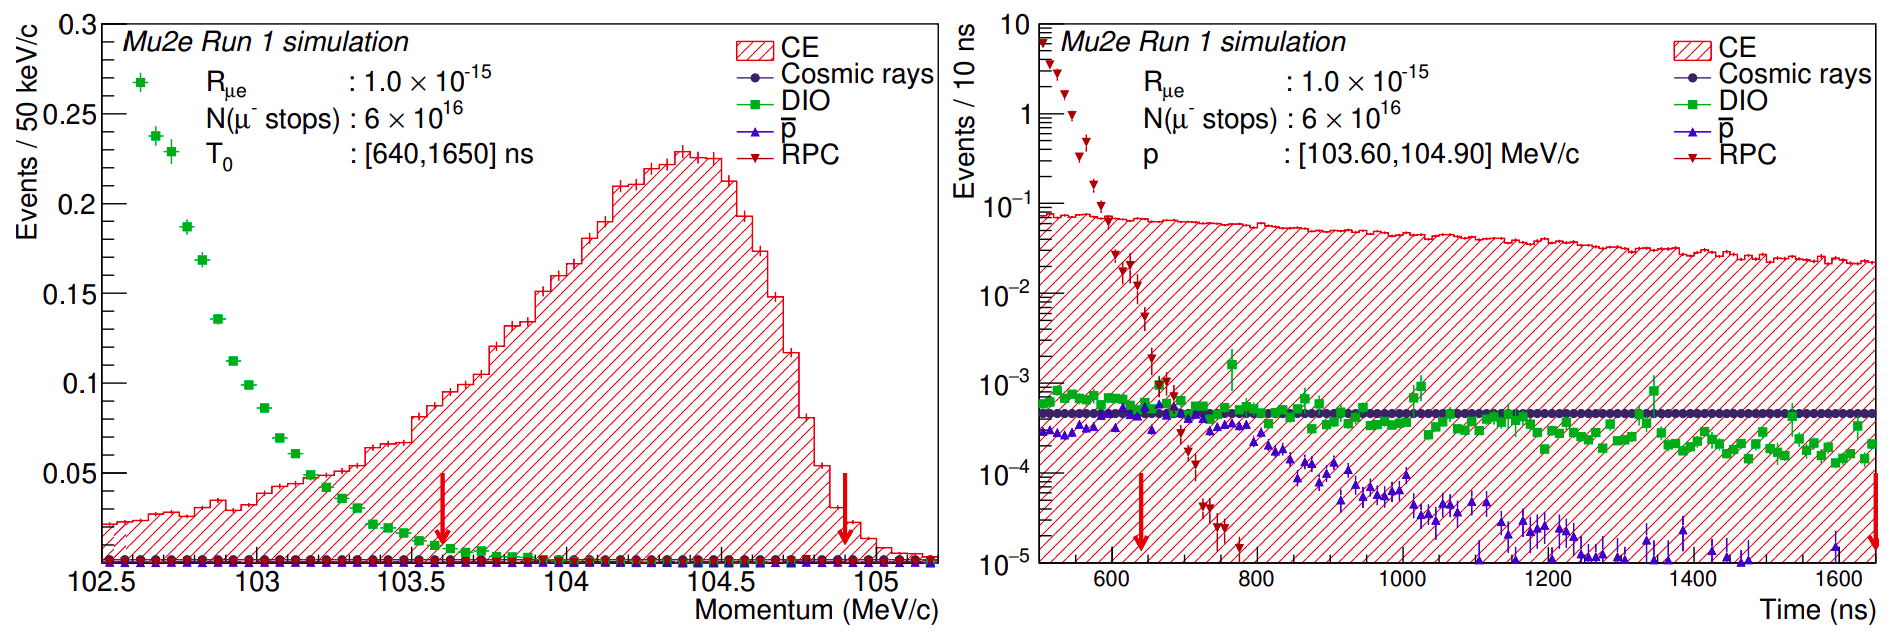
\includegraphics[width =0.93\textwidth]{figures/png/Screenshot_20240225_102708.png}
\caption[Mu2e simulated signal.]{Left: Momentum distribution of the CE signal and expected backgrounds. Right: Time distribution of the CE signal and expected backgrounds. The arrows show the signal region selected for the analysis, 103.60 $< \ p \ < $ 104.90 MeV/c and 640 $< \ T_0 \ < $ 1650 ns, Section \ref{pulsedprotonbeam}. The CE signal distributions correspond to $R_{\mu e} = 1 \times 10^{-15}$ \cite{universe9010054}.}
\label{fig:sensitivity}
\end{figure}
\section{Experimental setup}\label{setup}
Figure \ref{fig:mu2escheme} shows a schematic overview 
of the Mu2e experiment. The experiment uses 
a solenoid system to generate magnetic fields essential 
for its operations. The Production Solenoid (PS) surrounds 
the production target, while further downstream, the 
Transport Solenoid (TS) provides the magnetic field for 
the muon beamline. The TS, configured in an S-shape, 
incorporates collimators and proton absorbers. The ST is 
located at the beginning of the Detector Solenoid (DS). 
Proton absorbers surround the ST, not shown in the picture. 
The tracker and the calorimeter are housed in the DS, 
enabling momentum measurement and particle identification. 
Additionally, a Stopping Target Monitor (STM) positioned 
downstream at the DS's end, not shown, measures the rate of muons stopped in the ST.
Also not shown 
in the picture is the Mu2e CRV system which 
surrounds the DS and half of the TS. In the next sections, a 
more detailed description of systems of the Mu2e experiment will be given.
\begin{figure}[!h]
\centering
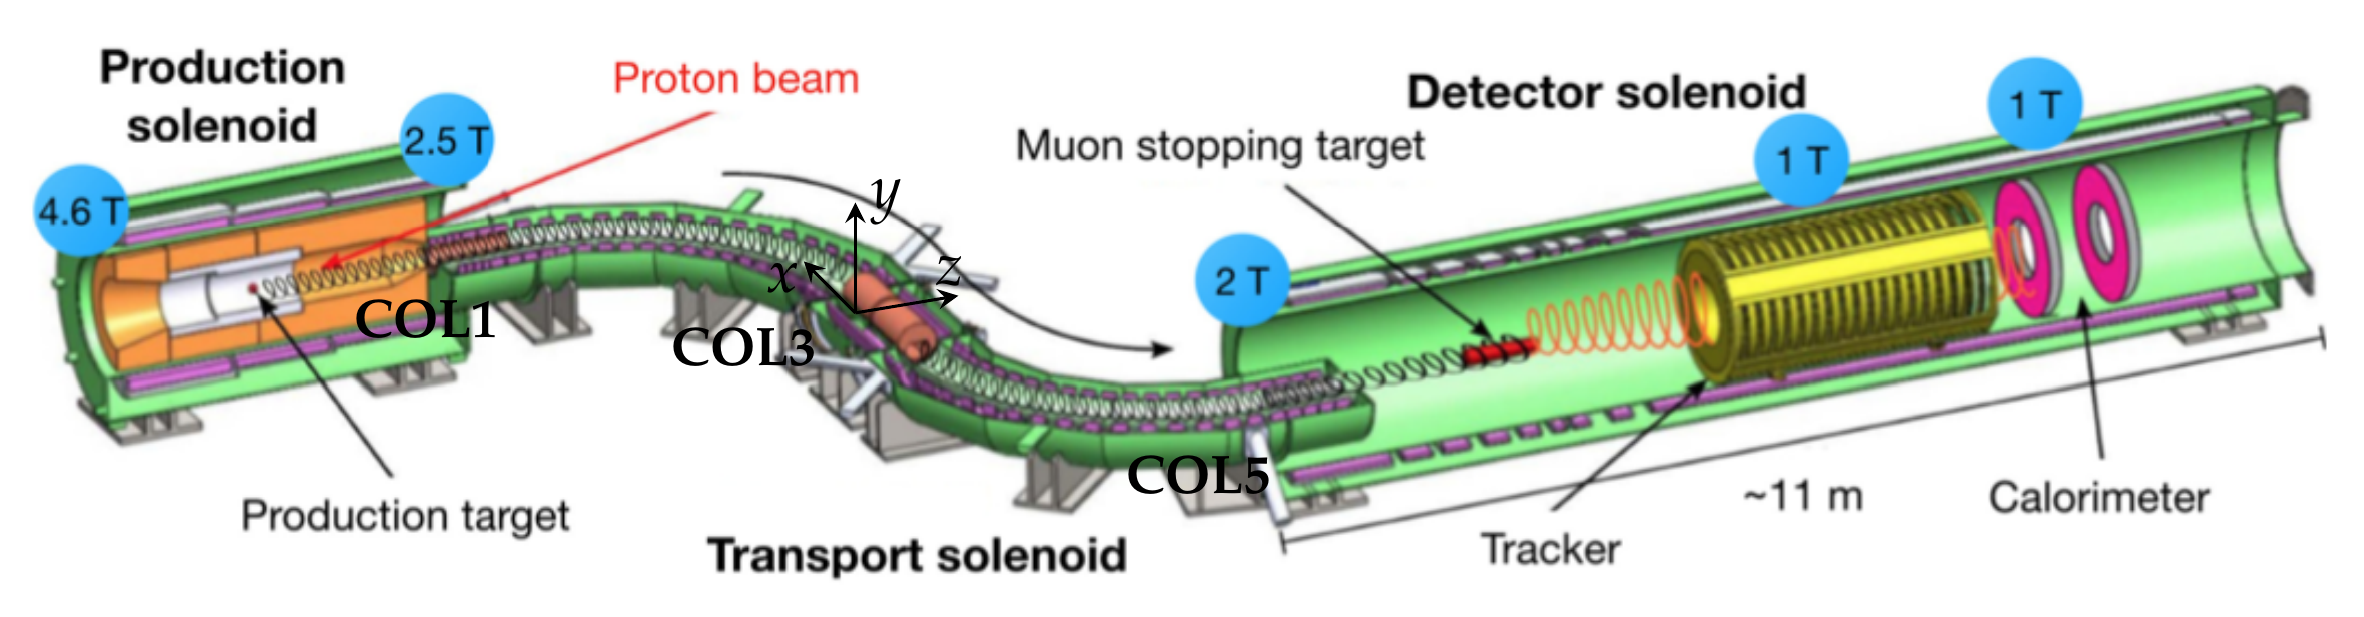
\includegraphics[width =\textwidth]{figures/png/Screenshot_20240301_143105.png}
\caption[The Mu2e apparatus.]{Schematic view of the Mu2e apparatus. The center 
of the Mu2e reference frame is located at the COL3 collimator center, its $y$-axis 
points upwards, the z-axis is parallel to the DS axis and points downstream, and 
the $x$-axis completes the right-handed reference frame \cite{universe9010054}.}
\label{fig:mu2escheme}
\end{figure}
\section{Accelerator system and the proton beam}\label{accel}
\subsection{Pulsed proton beam}\label{pulsedprotonbeam}
As previously discussed in Section  \ref{backgrounds}, the Mu2e experiment uses a 
pulsed proton beam.

The 8 GeV, 8 kW beam originates from the Fermilab Booster \cite{PhysRevAccelBeams.20.111003}. 
The proton pulses are separated by 1695 ns. Figure \ref{fig:accell} 
illustrates the Fermilab accelerator facilities involved in generating and delivering 
the pulsed proton beam. The Fermilab Booster delivers 8 GeV protons in 20 batches 
throughout a 1.4 s Main Injector cycle at 15 Hz, as shown in Figure \ref{fig:deliver}. 
Thus, the accelerator timeline is described using a fundamental time unit of 1 tick that corresponds to 66.7 ms.

\begin{figure}[!h]
     \begin{subfigure}[b]{0.4\linewidth}
         \centering
         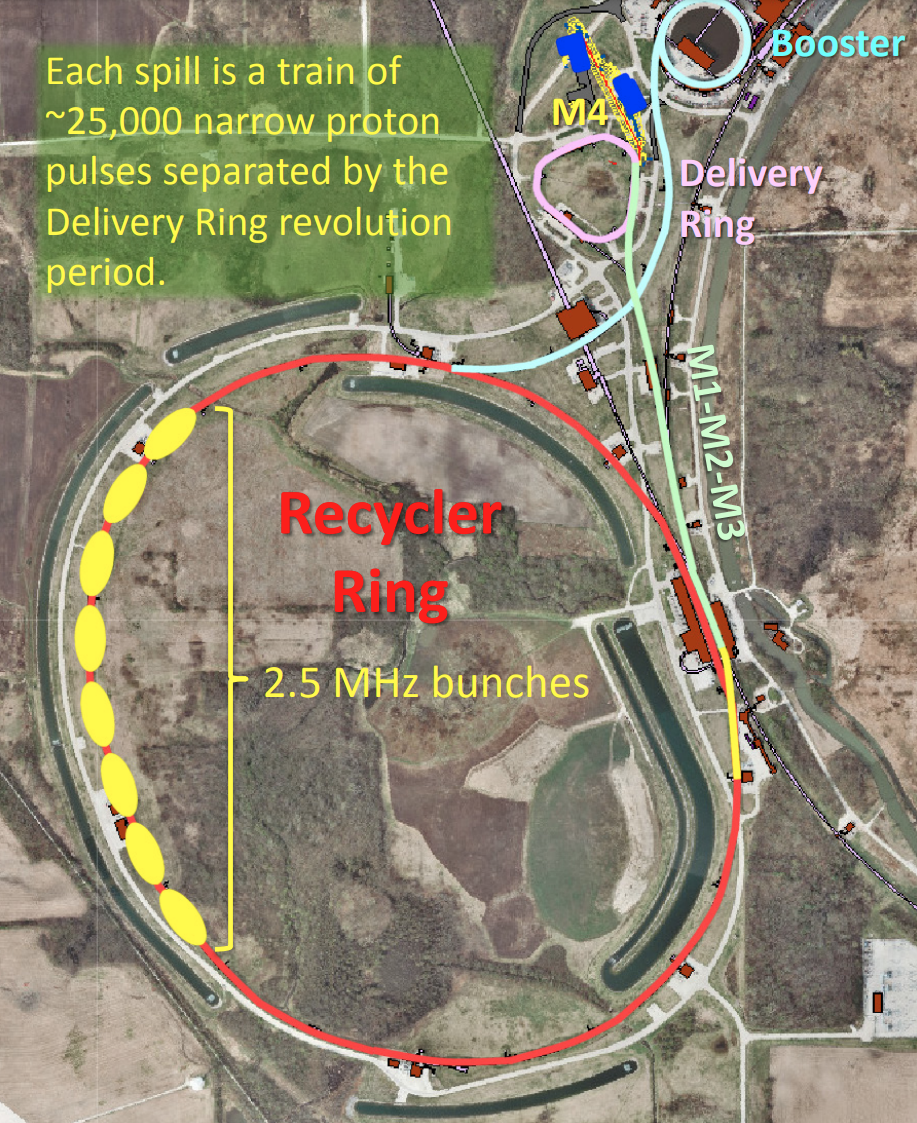
\includegraphics[scale = 0.3]{figures/png/Screenshot_20240301_151449.png}
         \subcaption{\centering Fermilab accelerator facilities involved in producing and delivering the pulsed proton beam.}
         \label{fig:accell}
     \end{subfigure}
     \begin{subfigure}[b]{0.7\linewidth}
         \centering
         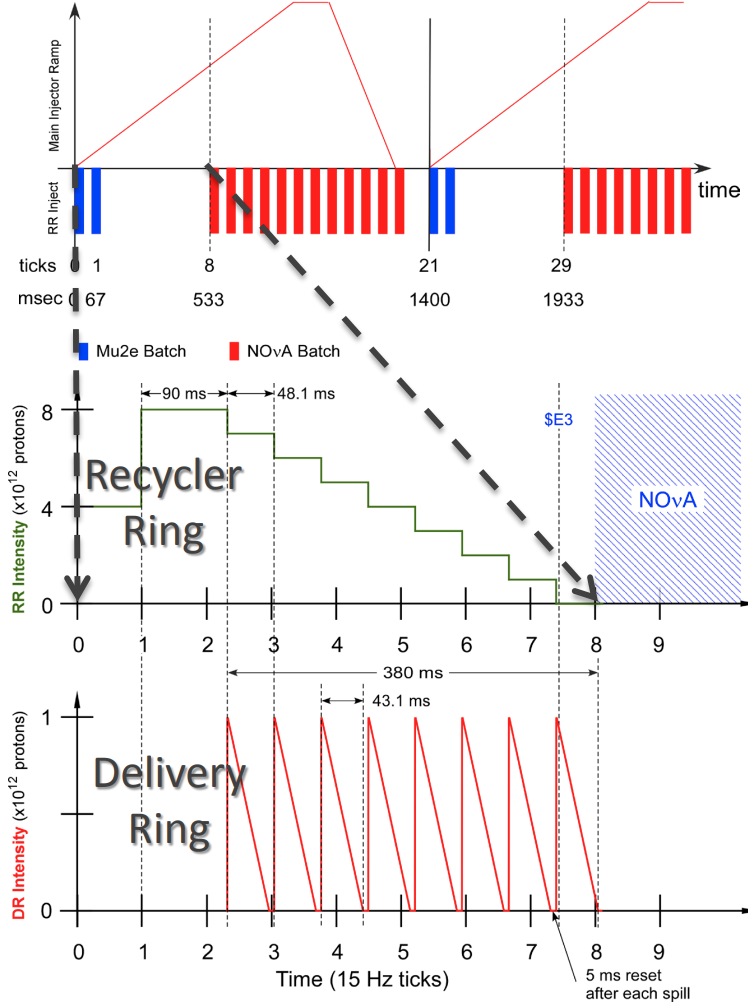
\includegraphics[scale = 0.39]{figures/png/Screenshot_20240301_151418.png}
         \subcaption{\centering Proton beam delivery to Mu2e.}
         \label{fig:deliver}
     \end{subfigure}
     \caption[The pulsed proton beam delivery.]{Pulsed proton beam delivery \cite{accelerator}.}
        \label{fig:three graphs1}
\end{figure}
The two Mu2e batches, represented by the two blue bars at ticks 1 (1BB) and 2 (2BB), are injected 
into the Recycler Ring, each containing $4 \times 10^{12}$ protons. The 
protons from these batches are reorganized within the Recycler using a 2.5 
MHz radio frequency (RF) system into 8 bunches. These bunches are then extracted 
individually from the Recycler and transported to the Delivery Ring every 48.1 ms, 
as shown in the middle part of Figure \ref{fig:deliver}. Once inside the Delivery 
Ring, a single bunch of $1 \times 10^{12}$ protons undergoes gradual extraction. 
This process results in the extraction of a small fraction of the bunch per revolution, 
delivered to the Mu2e experiment. The complete bunch is extracted over a span of 43.1 ms, 
across $\sim$25000 turns around the Delivery Ring, as shown in the bottom part of Figure \ref{fig:deliver}.
\begin{figure}[!h]
\centering
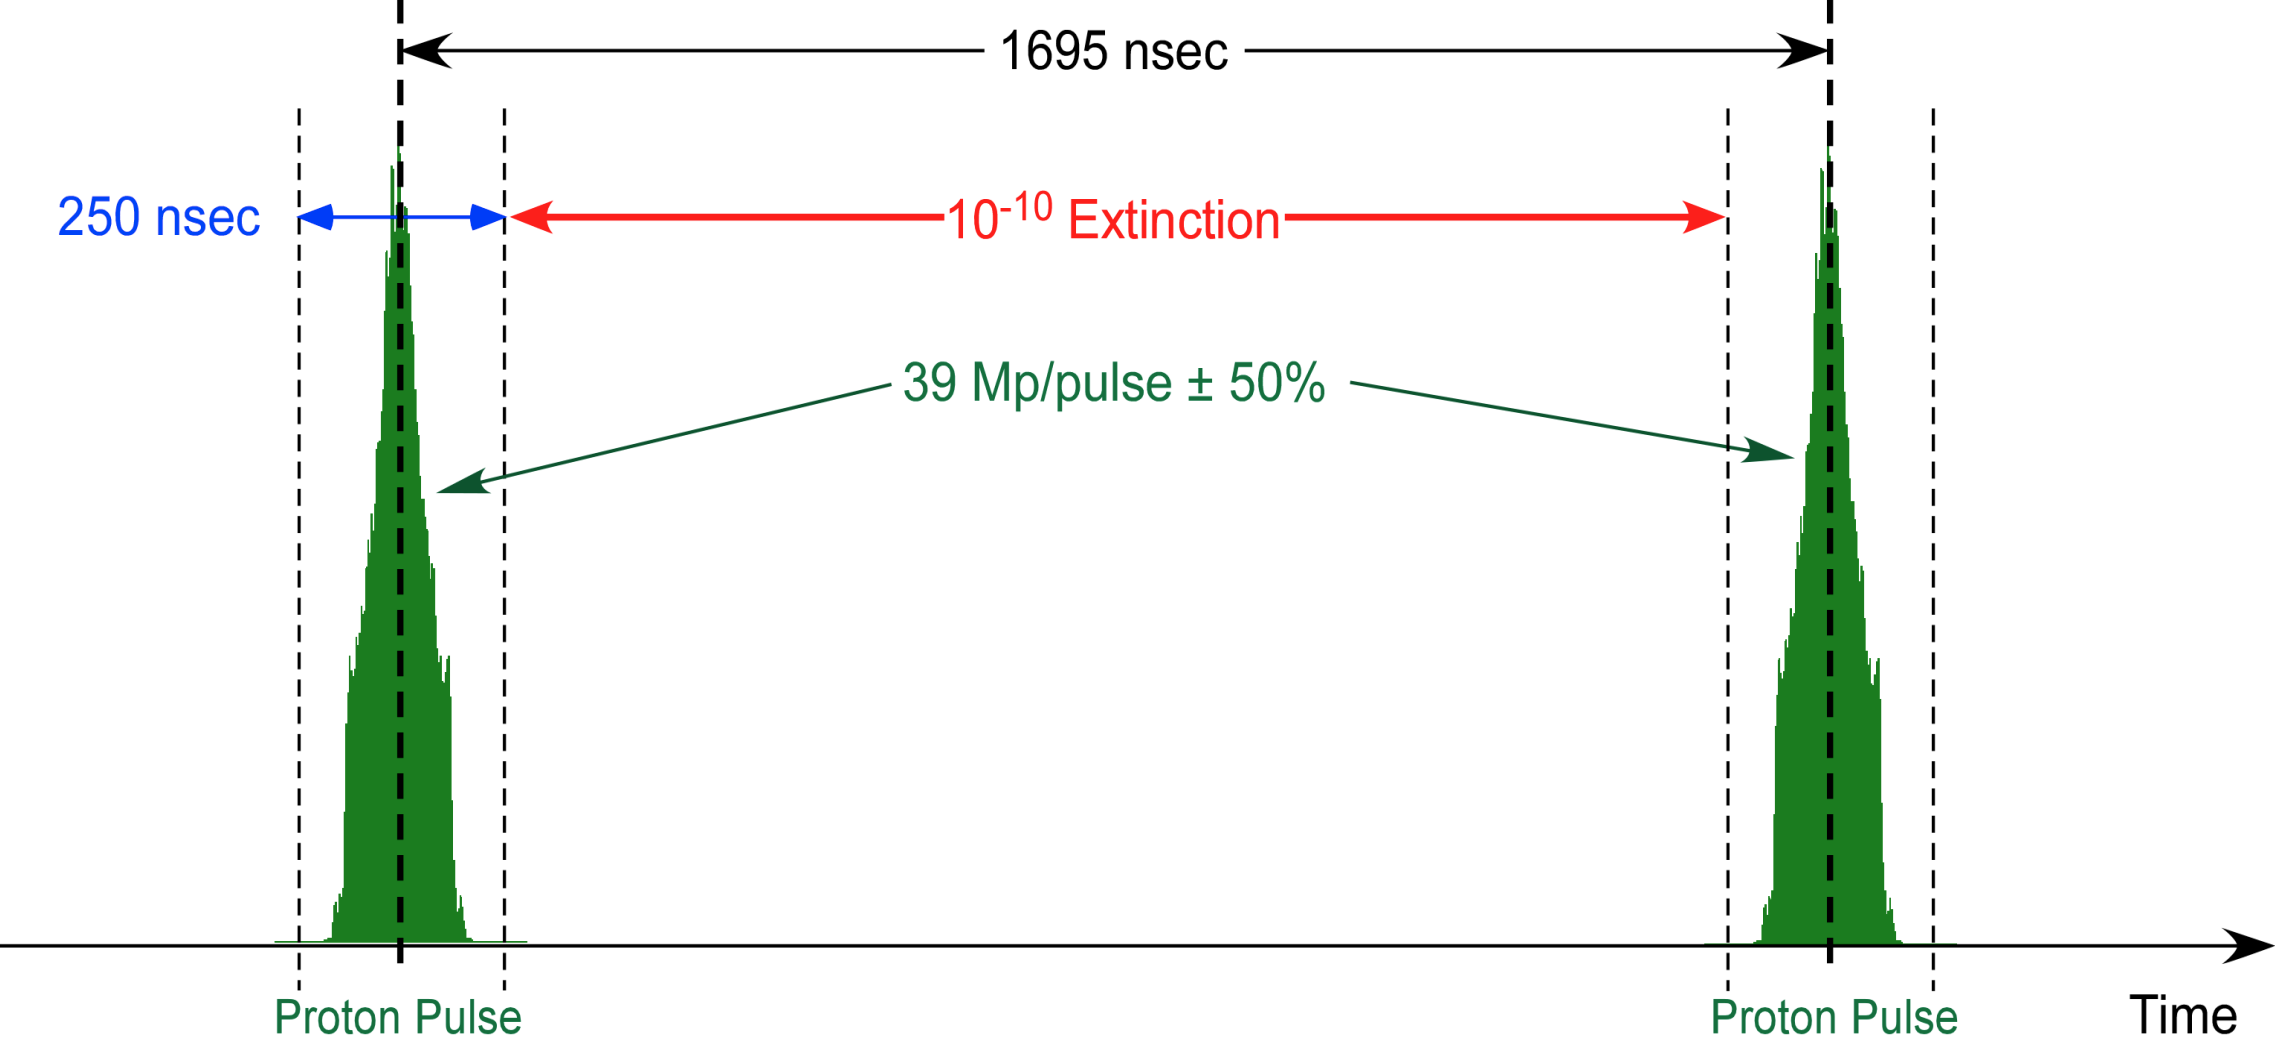
\includegraphics[width =0.8\textwidth]{figures/png/Screenshot_20240301_151148.png}
\caption[Proton beam profile.]{Proton beam profile at the Mu2e Proton Target \cite{accelerator}.}
\label{fig:beamprofile}
\end{figure}
Figure \ref{fig:beamprofile} illustrates the temporal 
profile of the beam at the PT. Consecutive 
proton pulses are spaced by 1695 ns. Each pulse lasts for 
250 ns and contains $(3.9 \pm 2.0 )\times 10^7$ protons. 
The 1695 ns pulse separation is highly advantageous for 
the Mu2e experiment. Figure \ref{fig:beamwindow} shows the beam pulse, 
the simulated pion flux, the muon capture rate on the ST 
and the muon decay rate. The active window for detecting 
CEs begins at $\sim$640 ns and extends for more or less 1 
$\mu$s. 

\begin{figure}[!h]
\centering
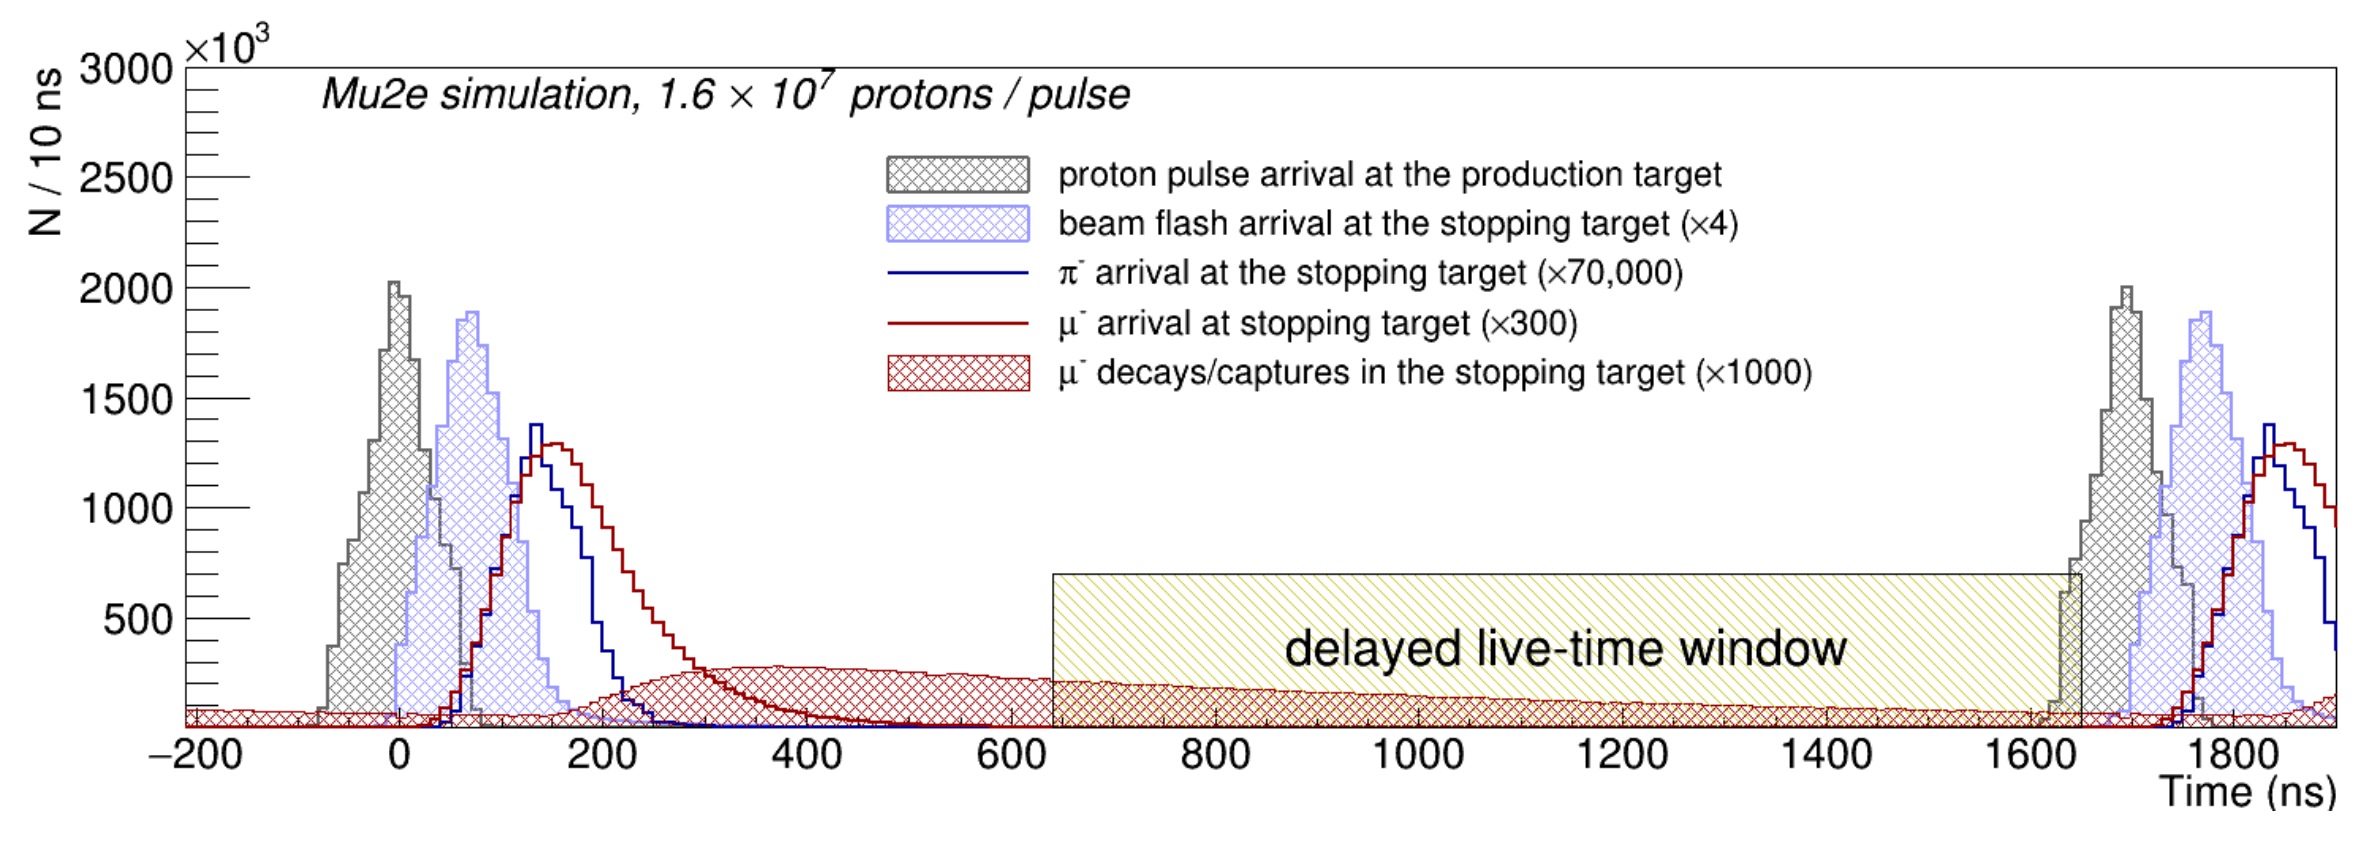
\includegraphics[width =0.9\textwidth]{figures/png/Screenshot_20240301_164649.png}
\caption[The Mu2e beam timing]{The Mu2e beam timing: the proton pulses arrive at the production solenoid every 1695 ns. A delayed live-time window can suppress the beam-related background \cite{universe9010054}.}
\label{fig:beamwindow}
\end{figure}
\subsection{Proton beam extinction and Extinction Monitor}
As mentioned in the previous section, the Mu2e experiment 
requires the extinction level of the incoming proton beam, to reduce backgrounds caused by out-of-time protons. 
The extinction rate, defined as the ratio between the 
number of out-of-time protons and the number of the in-time protons, should be lower than $10^{-10}$ \cite{bartoszek2015mu2e}. The structure of the beam 
leads to an extinction level $2.1 \times 10^{-5}$. To take into account the fact that some beam will 
leak out of two consecutive proton pulses, an Extinction 
Insert is deployed in the M4 beamline between the Delivery Ring and the Mu2e experiment.
The out-of-time beam particles are swept into a collimator system by an oscillating dipole, called AC dipole. These AC dipole 
offers an additional 
extinction factor of $5\times 10^{-8}$, reducing the 
overall extinction to $1.1 \times 10^{-12}$, leaving a margin of 10$^2$ \cite{accelerator}. An 
Extinction Monitor is positioned downstream of the 
production target along the proton beamline, as shown in Figure \ref{fig:extintion}. It monitors the 
extinction level of the proton beam and delivers a measurement with an accuracy of 10\%.

The Extinction Monitor consists of a collimator and magnetic filter 
system, a pixel telescope, a system of trigger scintillators and a range-stack. The collimator and 
magnetic filter system transport a small quantity of 
the particles generated at the production target to the Extinction Monitor. The pixel telescope 
tracks the trajectory of charged particles coming from 
the collimator. The pixel telescope consists of a permanent magnet and 8 scintillators, as shown 
in Figure \ref{fig:extintionmonitor}. The system uses a 
permanent magnet to separate two sets of four scintillator planes, allowing for momentum measurements 
of entering particles. The range stack is located further 
downstream from the pixel telescope. Steel absorber plates separate scintillators, distinguishing 
between hadrons and muons based on their penetrating capacity.
\begin{figure}[!h]
\centering
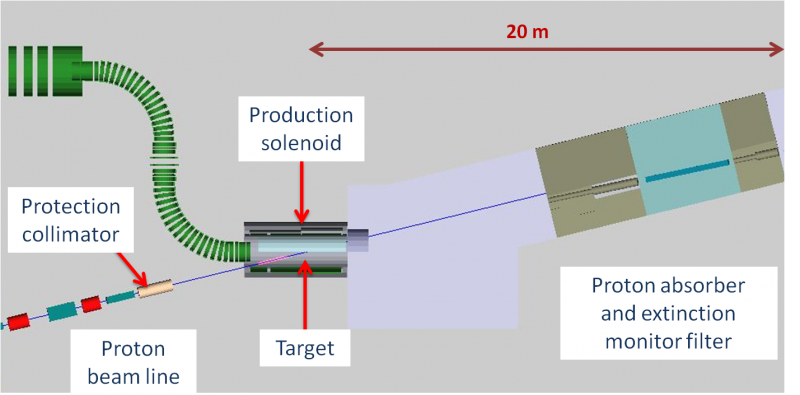
\includegraphics[width =0.8\textwidth]{figures/png/800px-Extinction_filter.png}
\caption[The Extintion Monitor location.]{The Extinction Monitor is located downstream of the
production target \cite{Prebys:IPAC2015-THPF121}.}
\label{fig:extintion}
\end{figure}
\begin{figure}[!h]
\centering
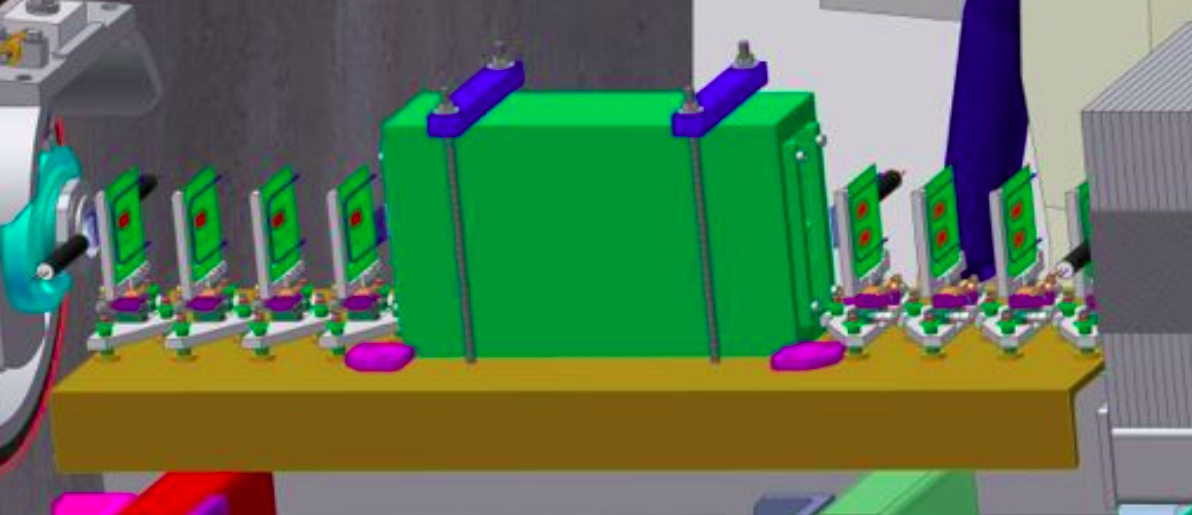
\includegraphics[width =0.7\textwidth]{figures/png/Screenshot_20240306_184720.png}
\caption[The Extintion Monitor.]{The tracking spectrometer of the Mu2e experiment, consisting of eight planes of pixel detectors and a permanent magnet spectrometer \cite{Prebys:IPAC2015-THPF121}.}
\label{fig:extintionmonitor}
\end{figure}
\subsection{Production Target}
The Mu2e production target (PT) is made of tungsten. 
The material was chosen because of its high 
melting point (3422 °C) and excellent resistance to deformation and corrosion.

It is positioned in the middle of the PS bore \cite{bartoszek2015mu2e}.
The tungsten core is embedded in a \textit{bicycle wheel} frame, 
suspended by the spokes.
The current design of the PT, shown in Figure \ref{fig:PT}, 
has circular rings at the end and its segmented core provides a better temperature 
dissipation. This design is expected to last for more than one year. The PT provides a muon yield of 0.0016 $\mu$/proton \cite{PT}.
\begin{figure}[!h]
    \centering
    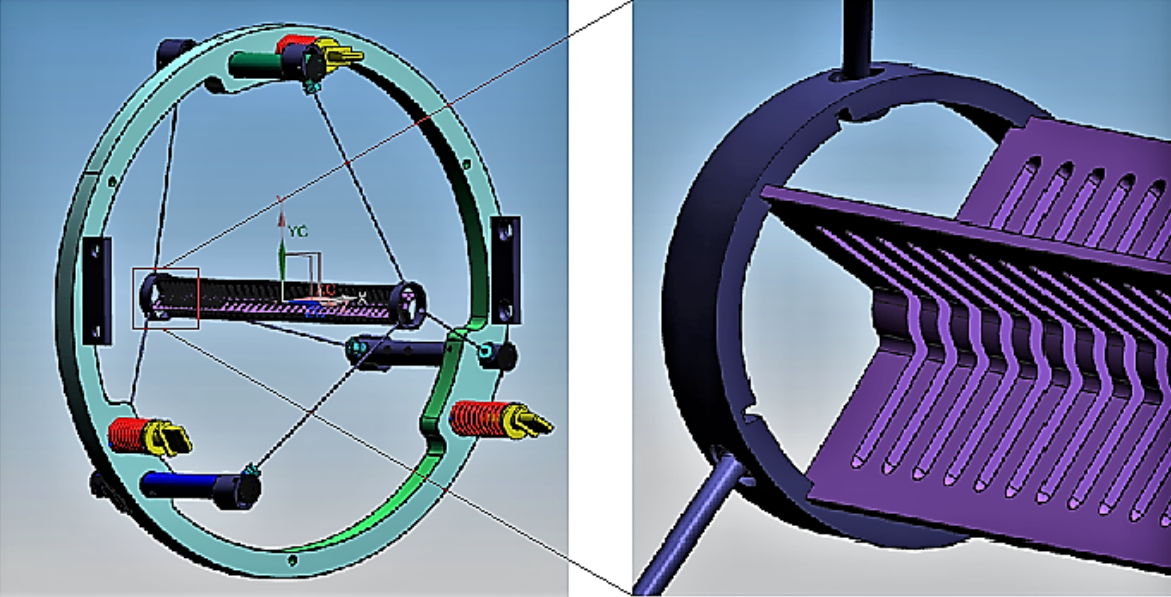
\includegraphics[width =0.7\textwidth]{figures/png/Screenshot_20240706_114229.png}
    \caption[The Production Target design.]{The design of the PT. Left: bicycle wheel 
      structure with the PT at the
    center. Right: zoom on the tungsten target.}
    \label{fig:PT}
\end{figure}

\section{Solenoids}
The principle of the Mu2e experiment is to use a sophisticated magnetic system
to form the high-intensity muon beam by collecting and filtering the particles emerging from the PT. 
It is composed of three parts: the \textbf{Production Solenoid} (PS), the \textbf{Transport Solenoid} (TS) 
and the \textbf{Detector Solenoid} (DS), shown in Figure \ref{fig:mu2escheme}. 
Each one is made of superconducting 
coils wound with aluminum stabilized Nb-Ti Rutherford cables.

The resulting magnetic field varies from 4.6 T at the upstream end of the PS 
to 1 T at the downstream end of the DS. 
The muons are guided towards the ST and the DS by lowering the magnetic field. 
Local magnetic field minima are avoided to avoid trapping particles in these areas. 
In the PS, the magnetic field decreases from 4.6 T to 2.5 T at the entrance of 
the TS. The large gradient helps to collect the secondary pions and muons and to 
direct them towards the DS. The magnetic field across the S-shaped TS changes its 
value only by a factor of 0.5 T. The shape of the TS allows to select charged particles 
and its dimension was set to avoid transmitting 
particles with large momentum. These particles either spiral with a large helical 
radius (large initial momenta perpendicular to the field) or cannot create an 
S-shaped bend (large initial momenta parallel to the magnetic field), resulting 
in collisions with solenoid walls or collimators. As particle drifts in the solenoid field is dependent on the particle charge,  
positively and negatively charged muons 
drift in opposite vertical directions and are separated, as explained in Appendix 
\ref{appendix1}. In the upstream part of the TS, Figure 
\ref{fig:collimators}, the positive (blue) and negative (red) muons 
are deflected downwards and upwards respectively. Positive muons are stopped in 
collimators COL3u and COL3d. The TS is long enough for pion decay, suppressing 
RPC backgrounds.
The magnetic field in the first half of 
the DS is reduced from 2 T to 1 T. In a smoothly gradient field, the adiabatic 
invariance of the magnetic flux can be used. Assuming a constant $p^2_\perp/B$, there is:
\begin{equation}
    v^2_{\parallel}=v^2_0-v^2_{\perp 0}\frac{B(z)}{B_0}
\end{equation}
Here, $\perp$ is referred with respect to the magnetic field $B$ and $\parallel$ is 
referred to the $z$ direction. The subscript 0's indicates the initial state. 
The gradient pitches electrons forward into the tracker's acceptance. 

The second half of the DS containing the tracker and the calorimeter has a 
uniform magnetic field of 1 T.

\begin{figure}[!h]
\centering
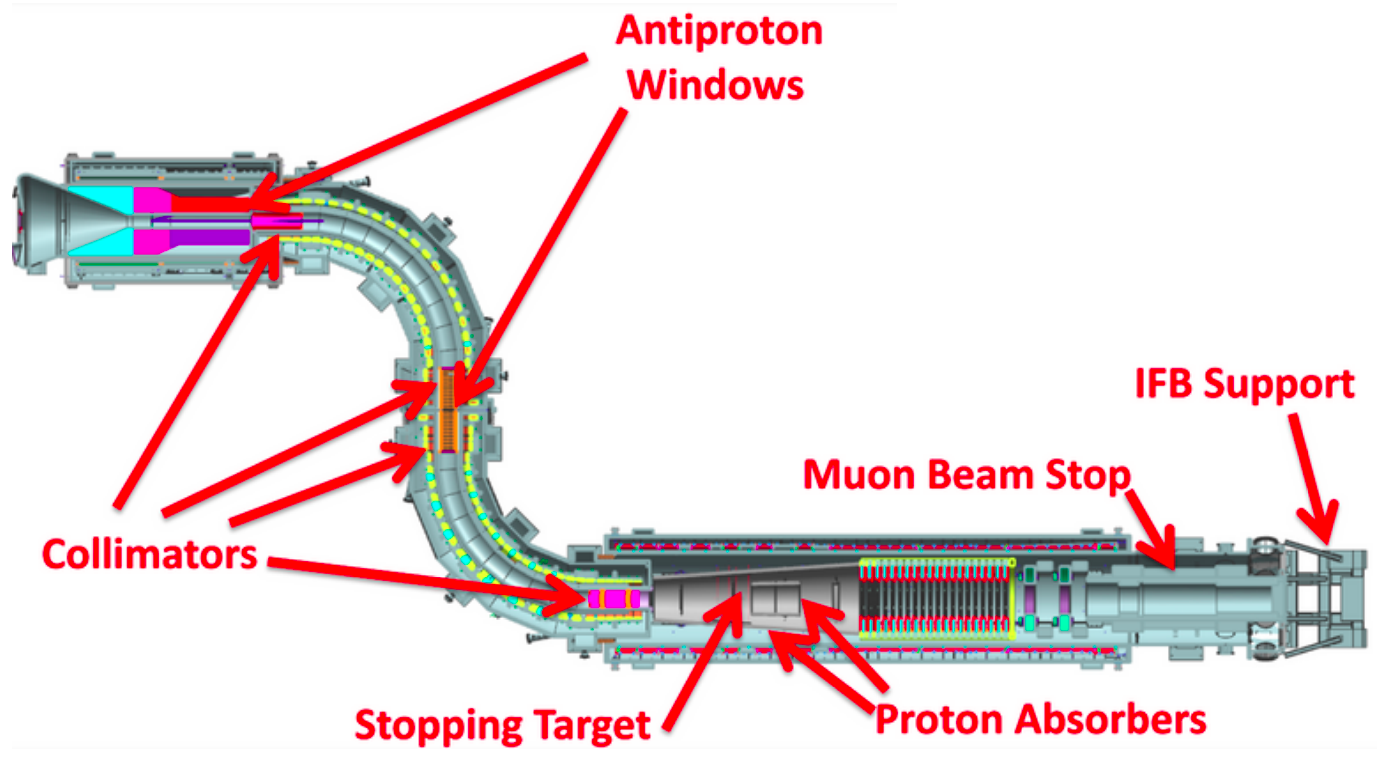
\includegraphics[width =0.7\textwidth]{figures/png/Screenshot_20240303_152845.png}
\caption[The muon beamline.]{The muon beamline, composed of the Production Solenoid (PS), 
the Transport Solenoid (TS) and the Dector Solenoids (DS) \cite{ginther}. 
}
\label{fig:muonbeamline}
\end{figure}


\subsection{The Production Solenoid}
The Production Solenoid (PS) (4 m long), shown in Figure \ref{fig:PS}, collects pions, 
kaons generated by the interactions between the 8 GeV proton beam and the production target. 
The magnetic field gradient allows to collect also part of the particles 
emitted along the proton beam direction, improving the stopped muon yield.
It is composed of Nb-Ti superconducting cables stabilised with Al 
and cooled by liquid helium. To avoid damages to the superconducting cables and
to the cooling system a bronze heat and radiation shield is built inside the solenoid.
The magnetic field is 4.6 T at the end of the PS and decreases almost linearly to 2.5 T at the
junction with the TS.
\begin{figure}[!h]
    \centering
    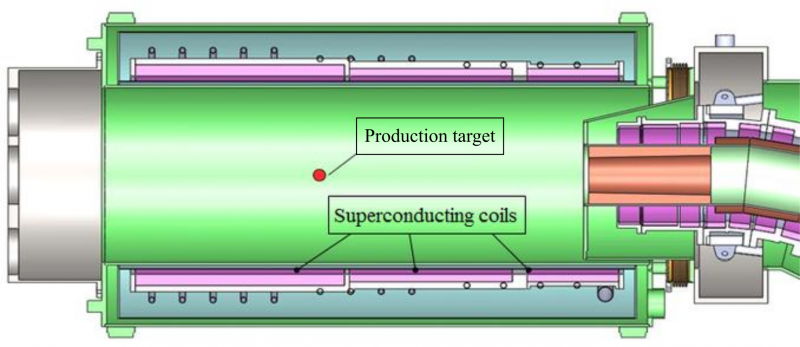
\includegraphics[width =0.7\textwidth]{figures/png/800px-Production_solenoid.png}
    \caption[The cross-section of the production solenoid.]{Cross-section of the production solenoid \cite{6376120}.
    The production target is placed approximately at the center of the superconducting coils.}
    \label{fig:PS}
    \end{figure}
\subsection{The Transport Solenoid}
The S-shaped TS is composed of a series of wide aperture superconducting
solenoid rings. It also contains a set of collimators and absorbers to provide charge and 
momentum selection and reduce the flux of antiprotons.
A thin window assembly is installed at the 
beginning of the TS and also between the rotatable collimators to absorb antiprotons in 
the beam. 

It is divided in five parts. 

The first one is called TS1 that contains the first collimator (COL1), 
Figure \ref{fig:collimatorsshape}, made of copper wedges. 
It filters particles from their momentum and reduces the radiation damage for coils of the 
upstream part of the TS (TSu). 

The TS2 contains a toroidal field in order to create a 
vertical displacement of the charged particles,
according to their charge and momentum.
Neutral particles, that are not sensitive to the magnetic 
field are not transported to the next section.

In TS3, negative muons are selected with two rotatable collimators (COL3u and COL3d, 
shown in Figure \ref{fig:collimatorsshape}). 
The rotatable feature allows selection of $\mu^-$'s instead of $\mu^+$'s, which can 
be used for detector calibration. 

The TS4 is the second toroid section of the TS and its role is 
to collimate the beams on the TS axis.

TS5 connects TS with DS and it contains a collimator (COL5), 
Figure \ref{fig:collimatorsshape}, made of polyethylene, 
which will serve as a shield from antiprotons.

It is linked to the DS 
and matches its field to provide the best beam transmission.


\begin{figure}[!h]
    \centering
    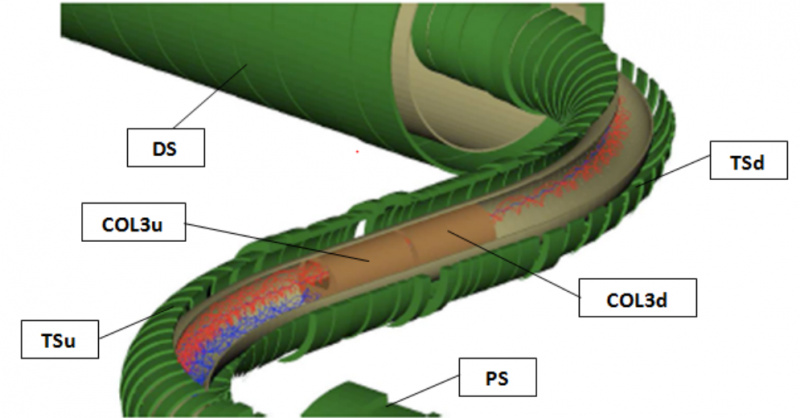
\includegraphics[width =0.7\textwidth]{figures/png/800px-MuonBeamlineCollimators2.png}
    \caption[The Transport Solenoid and the collimators.]{The schematic representation of the TS and the collimators COL3u and 
    COL3d showing the offset apertures in those collimators. The 
    upper spiraling negative muons (red) pass through the aperture while 
    the positive muons (blue) are stopped by these collimators \cite{tsview}.}
    \label{fig:collimators}
    \end{figure}
    \begin{figure}[!h]
        \centering
        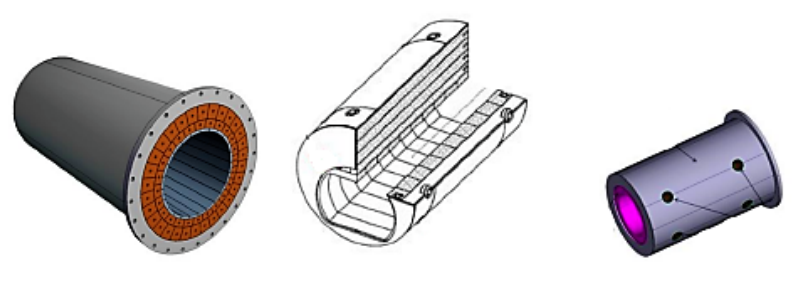
\includegraphics[width =0.7\textwidth]{figures/png/Screenshot_20240706_120535.png}
        \caption[The design of the collimators in the TS.]{Design of the collimators in the TS. From left to right: COL1, COL3u and COL3d
        and COL5.}
        \label{fig:collimatorsshape}
        \end{figure}

\subsection{The Detector Solenoid}\label{detectorsolenoid}
The DS, shown in Figure \ref{fig:DS}, is a cylindrical system of approximately 11 m in 
length and 2 m in radius, which houses the ST, 
the proton absorber, the tracker and the calorimeter. 
\begin{figure}[!h]
    \centering
    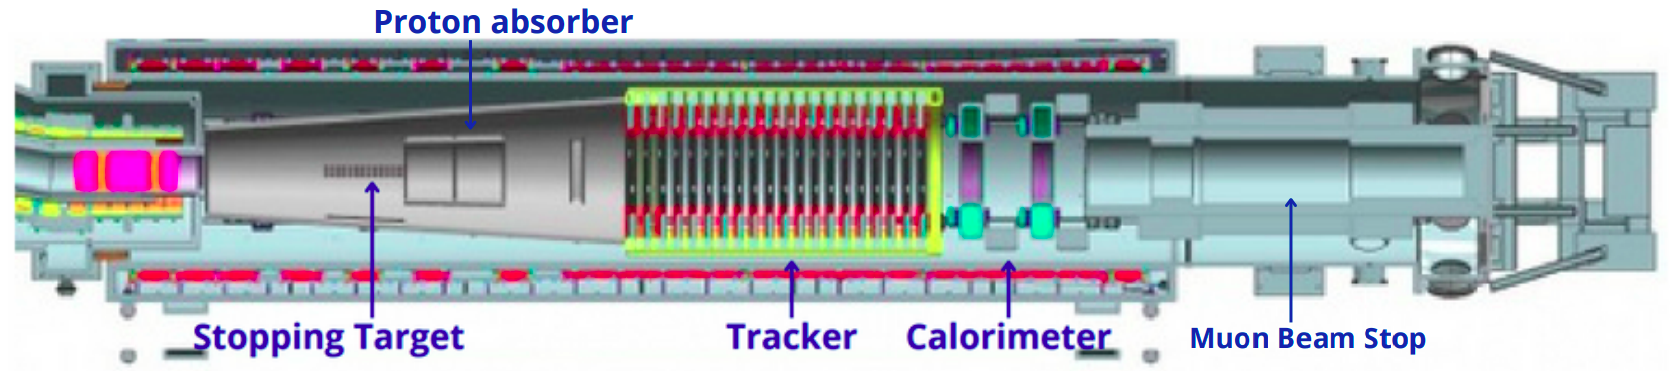
\includegraphics[width =0.8\textwidth]{figures/png/Screenshot_20240306_225639.png}
    \caption[The structure of the Detector Solenoid coils and cryostat.]{Overall structure of the DS coils and cryostat \cite{bobbb}.}
    \label{fig:DS}
    \end{figure}
The system is divided into two sections: a 4 m gradient section following the TS, 
where the magnetic field decreases linearly from 2 T to 1 T, and a 6 
m spectrometer section. 

The gradient region drives the CE 
inside the tracker acceptance, while the low momentum particles 
are driven to the low radius region that is not covered by detectors.  

In the spectrometer region, the uniform magnetic field allows a precise 
measurement of the particle momentum. 

The DS is straight, differently from the COMET experiment. This allows 
to detect both $e^+$ and $e^-$, with the disadvantage that the detectors are exposed to the 
beam flash and to protons and neutrons produced by the muon
nuclear capture in the ST.

A series of absorbing materials inside the DS, shown in 
Figure \ref{fig:absorbersDS}, is used to suppress 
the rate of protons and neutrons that can generate spare hits in the 
tracker:
\begin{itemize}
    \item \textbf{Transport Solenoid downstream absorber (TSdA)}: this 
    polyethylene disk-shaped absorber is designed to shield against neutron radiation. 
    Simulations predict it will reduce the hit rate in the calorimeter by approximately 30\% 
    while having a minimal impact (around 0.2\%) on electron acceptance;
    \item \textbf{Inner Proton Absorber (IPA)}: this is a thin (0.5 mm) conical 
    frustum made of low $Z$-material. It aims to reduce the rate of protons produced 
    in muon nuclear capture (around 0.03 per captured muon) while minimizing the 
    energy loss of CEs;
    \item \textbf{Outer Proton Absorber (OPA)}: another conical frustum with a 
    thickness of 20 mm, serving the same purpose as the IPA.
\end{itemize}
\begin{figure}[!h]
    \centering
    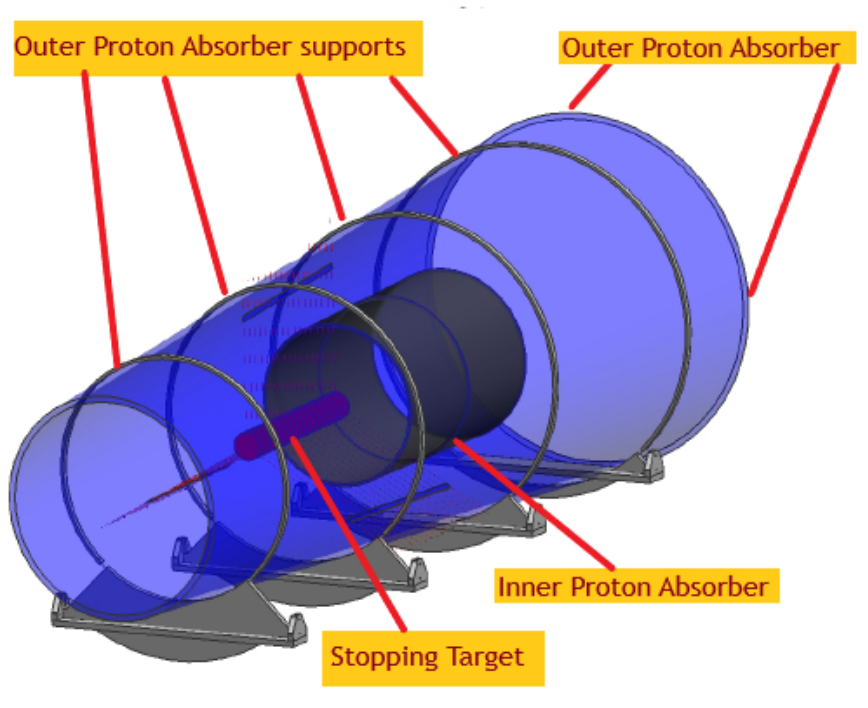
\includegraphics[width =0.5\textwidth]{figures/png/Screenshot_20240706_132949.png}
    \caption[The structure of the inner and outer proton absorber.]{The structure of the inner and outer proton absorber.}
    \label{fig:absorbersDS}
    \end{figure}




\section{Stopping Target}
The Mu2e ST, Figure \ref{fig:ST}, is 
composed of 37 annular aluminum foils of 75 mm of radius with a purity of 
above 99.99\% \cite{bobbb}. The foils are 100 $\mu$m thick to minimize energy losses of the CEs. This design 
narrows the reconstructed CE momentum distribution 
and separates it from the DIO electron momentum distribution. 
The disks have an internal hole of 21 mm of radius.
The annular design minimizes interactions with the beam electrons, reducing the radiation load by $\sim$30\%.

The central hole does not affect the target capacity to halt muons, 
which move in helical patterns. The space between each disk is
22.2 mm, bringing the total lenght of the ST to $\sim$80 cm.
Muons passing through the hole of an upstream foil will stop in a downstream layer. 
The design of the ST has been chosen by considering two 
conflicting physical requirements. Firstly, the target must be thick enough 
to stop a significant fraction of the muons, with the current version achieving 
an indicative stopping fraction of 30\%.

Secondly, the target must be thin 
enough to control the energy loss of the CEs, which is why 
the target has a segmented geometry.
\begin{figure}[!h]
    \centering
    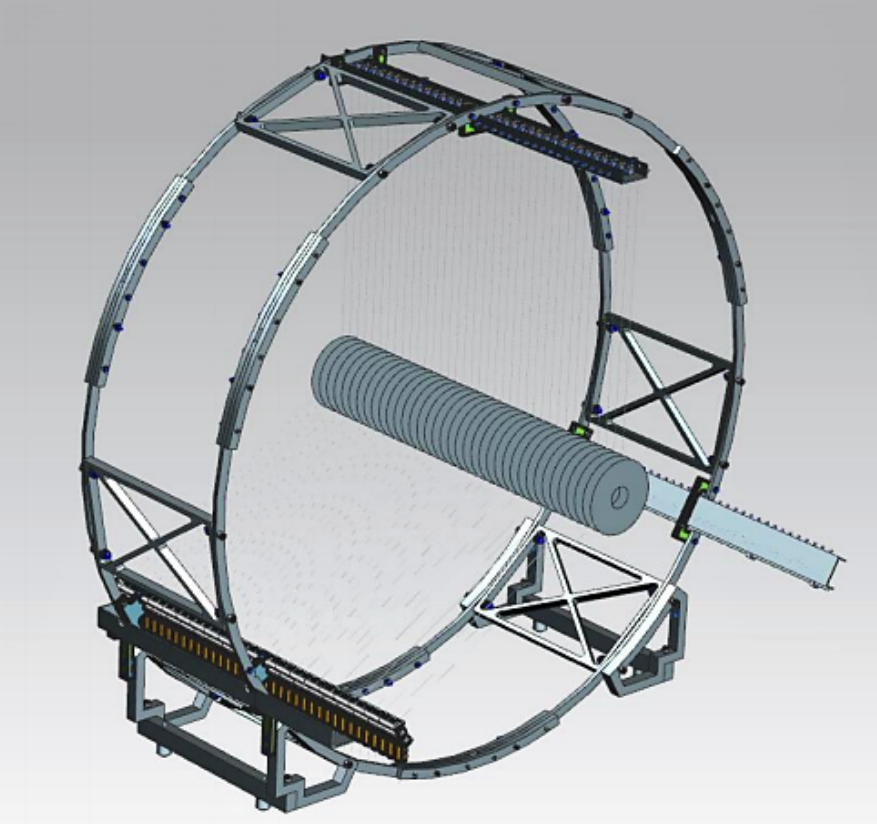
\includegraphics[width =0.5\textwidth]{figures/png/Screenshot_20240706_122723.png}
    \caption[The Stopping Target design.]{The ST design. 
    Each disk is supported by three cables not shown in the picture }
    \label{fig:ST}
\end{figure}

There are various factors to consider while selecting aluminum as the ST material. 
First, as described in Section \ref{backgrounds}, the aluminum 
target has a lower RMC background. Moreover, the muonic aluminium 
atom has a quite long lifetime, as shown in Figure \ref{fig:muonicatom}. 
The long lifetime allows separation between prompt backgrounds and a 
live window with a good decay rate. The muon DIO endpoint energy, 
further, depends on the type of nucleus, as shown in Figure \ref{fig:endpoint}. 
Aluminum has a high endpoint energy, so when muons are captured on other 
detector materials with a higher atomic number $Z$, they have lower 
endpoint energies and do not contribute to background. For these reasons, aluminum is a 
suitable ST material for muon-to-electron conversion searches.
Moreover, the branching ratio ($BR$) of the conversion varies 
depending on the ST material due to differences in atomic number 
($Z$) and mass number ($A$). By comparing $BR$s on different nuclei 
normalized to aluminum, it is possible to identify the dominating 
operator type, such as scalar ($S$), dipole ($D$), vector of 
transition charge radius type and vector of effective $Z$-penguin type, 
($V(\gamma)$) and ($V(Z)$) respectively. 
Despite challenges in separating prompt backgrounds from 
signals due to short lifetimes of muonic atoms, 
materials with higher $Z$ offer better model differentiation. 
If the Mu2e experiment observes conversion signals, a subsequent search 
could make use of titanium as the ST. A more detailed discussion can be 
found in \cite{PhysRevD.80.013002}, \cite{PhysRevD.76.059902} and 
\cite{abusalma2018expression}.


\begin{figure}[!h]
    \centering
    \begin{subfigure}[t]{0.5\textwidth}
        \centering
        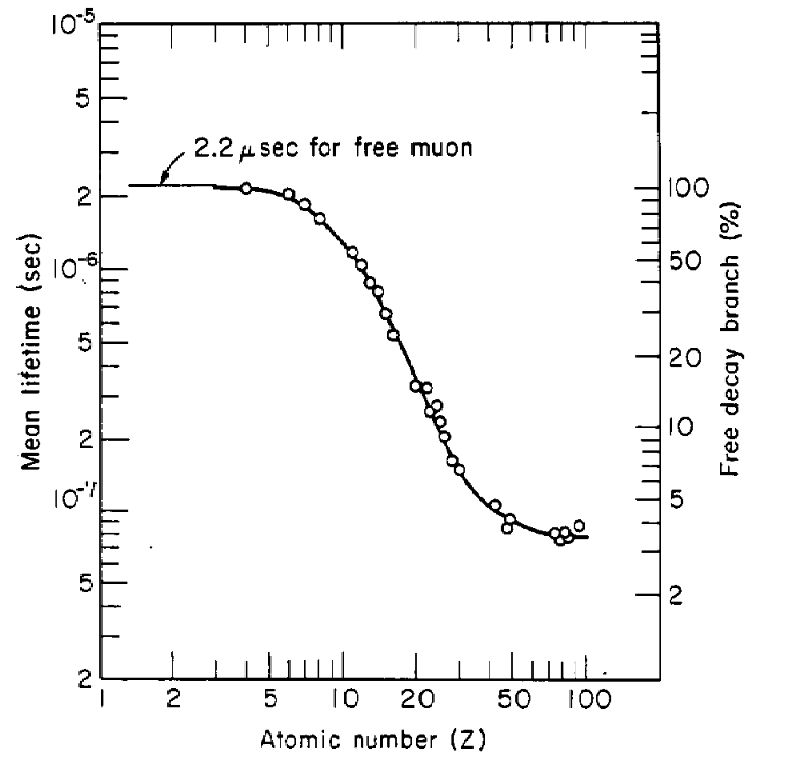
\includegraphics[width=0.85\textwidth]{figures/png/lifetime_mu_matter.png}
        \caption{}
        \label{fig:muonicatom}
    \end{subfigure}%
    ~ 
    \begin{subfigure}[t]{0.5\textwidth}
        \centering
        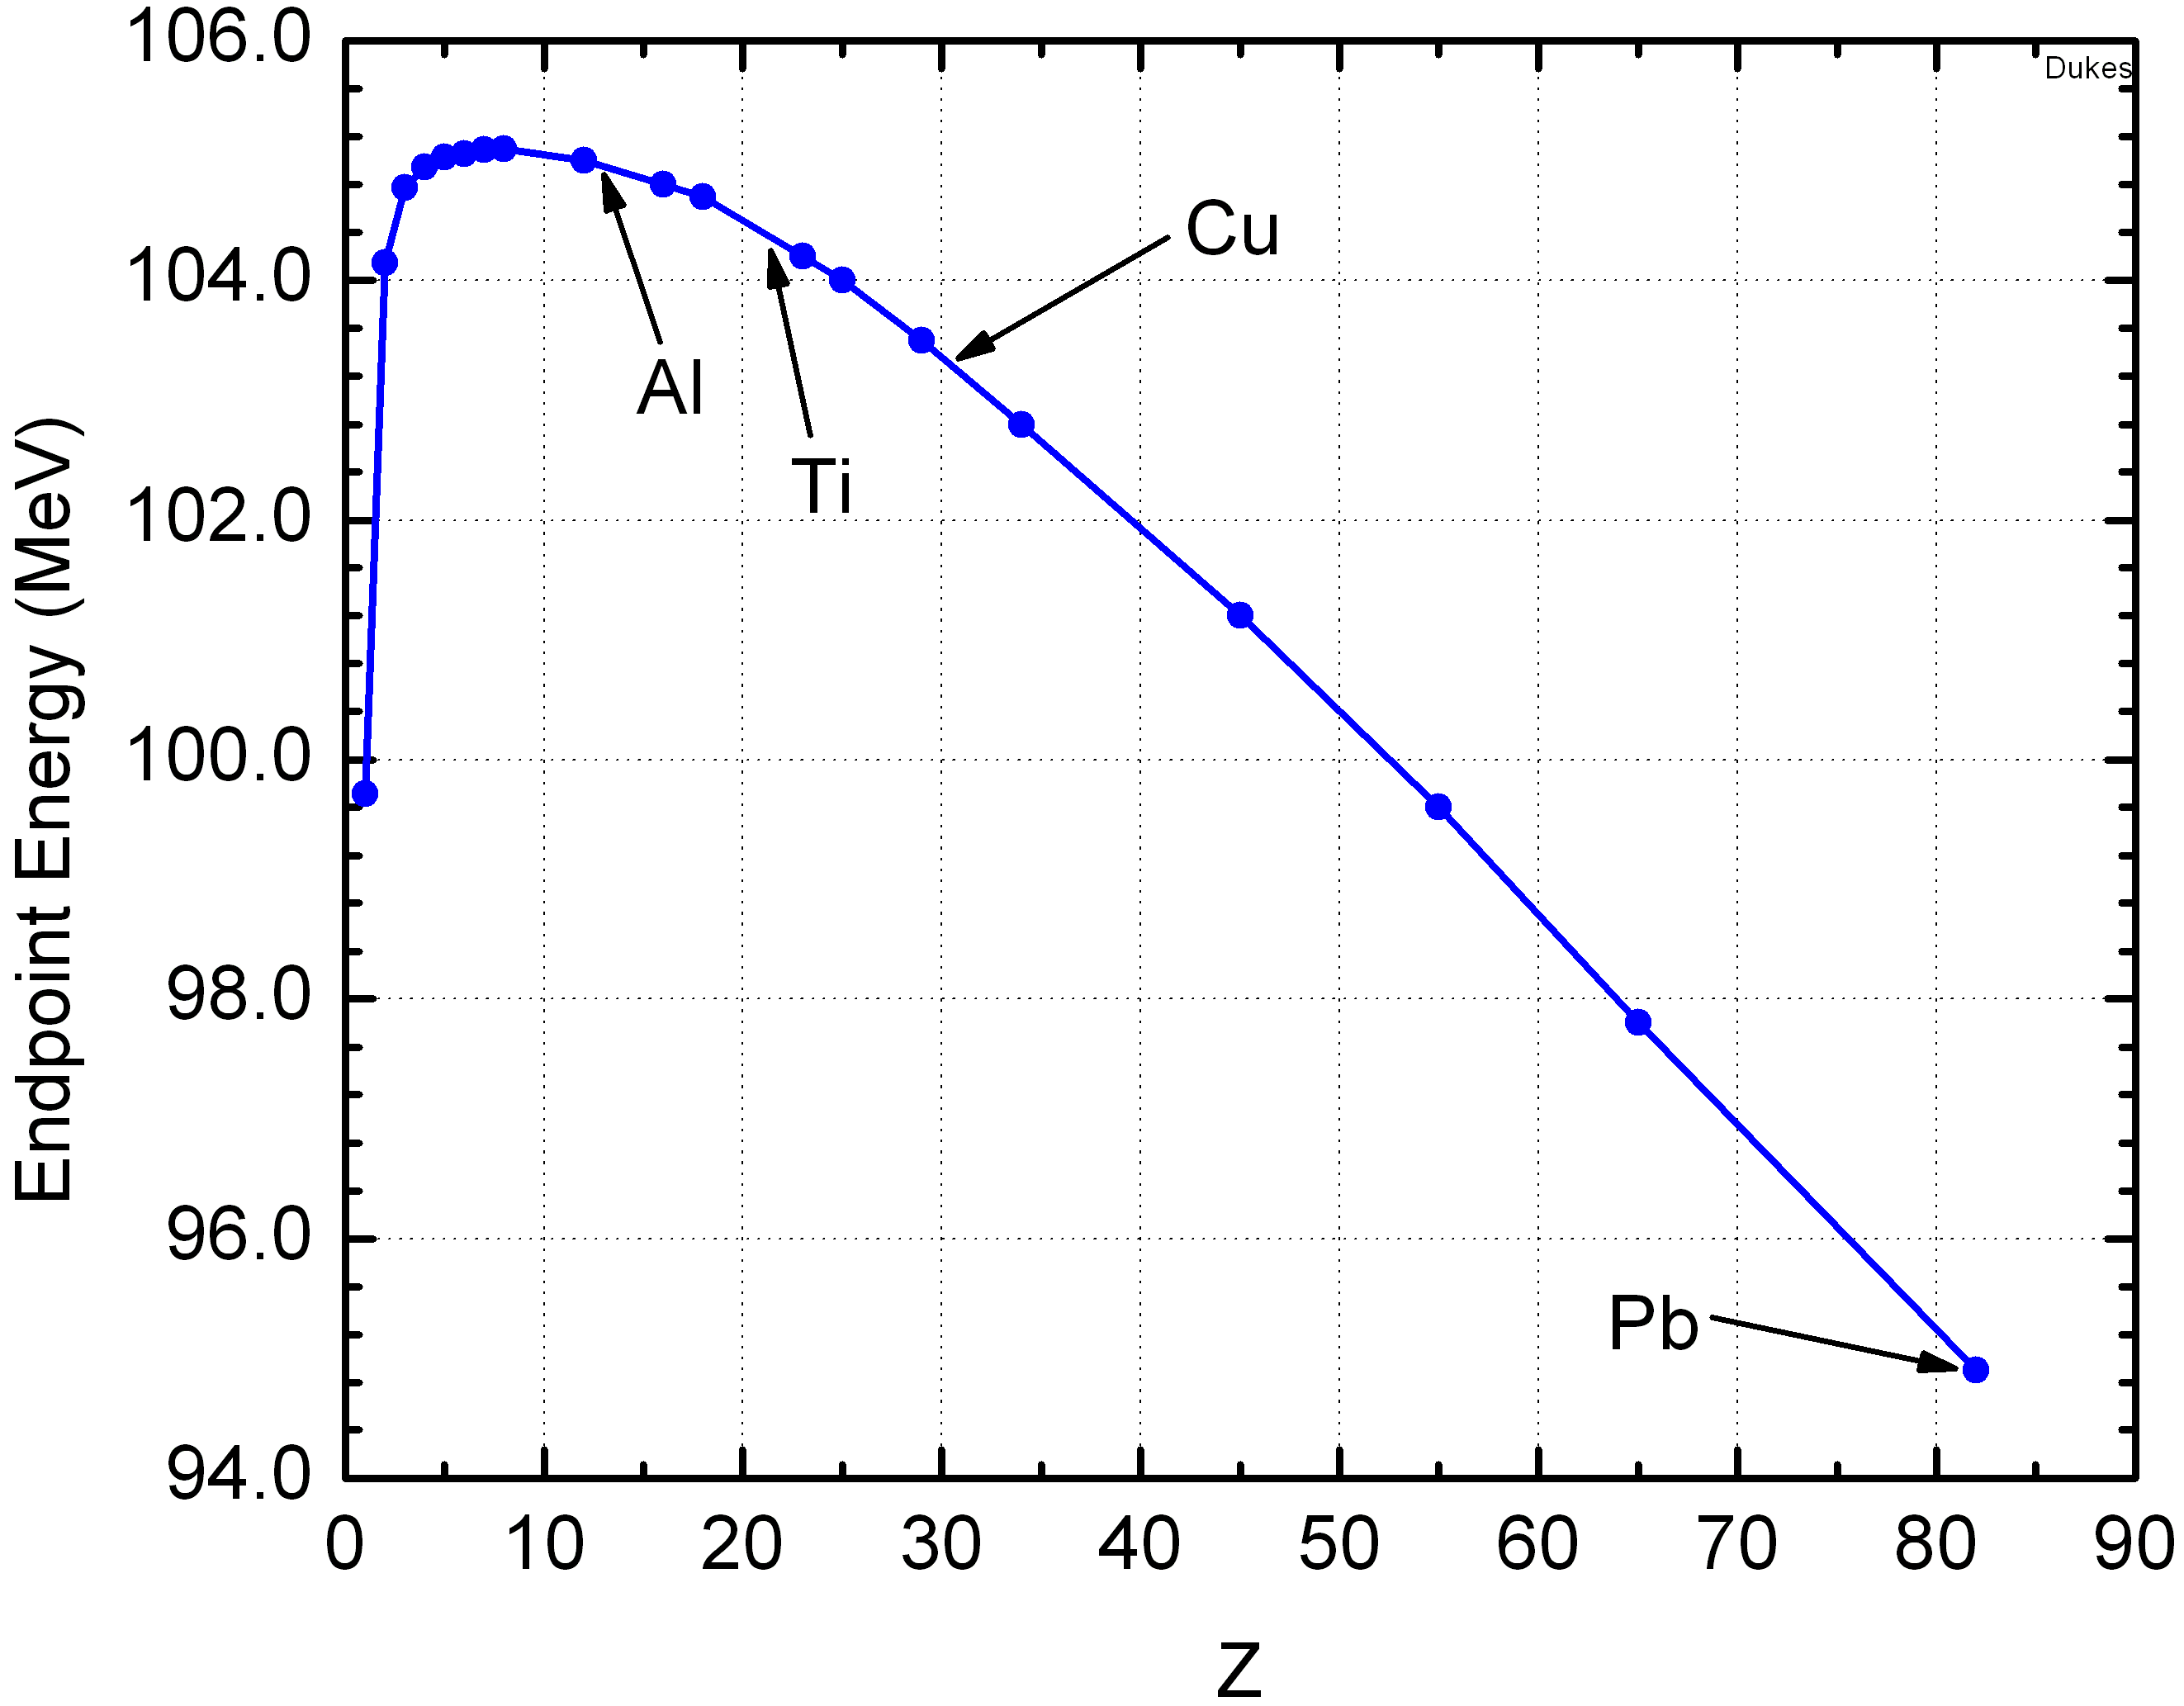
\includegraphics[width=0.85\textwidth]{figures/png/endopint.png}
        \caption{}
        \label{fig:endpoint}
    \end{subfigure}
   \caption[The muonic atom mean lifetime and muonic free decay fraction. The dependence 
   of the electron energy spectrum endpoint
   on the DIO.]{(a) The dependence of the mean lifetime and free decay fraction 
   of the muonic $1s$ state on the atomic number of the nucleus to which 
   the negative muon is bound \cite{TYamazaki_1975}, and (b) 
   the dependence of the electron 
   energy spectrum endpoint on the DIO \cite{dukes}.}
    \label{fig:2imins}
  \end{figure}
\section{The Mu2e detectors}
Mu2e makes use of a set of complementary detectors to 
measure particles momentum and energy. These detectors 
are annular and situated within a solenoidal magnetic field of 
approximately 1 T along the $z$-axis, which aligns with 
the direction of the muon beam. This distinctive geometry 
is highly effective in reducing background, as it allows 
the passage of particles produced during muon capture, 
remnant beam, and electrons from the initial proton collision to the beam dump without striking
the detector elements, that otherwise would cause excessive instantaneous detector 
occupancy and accumulated radiation damage. 
Most decay muons are tipically too low momentum 
to exit the central region, preventing them from reaching the detector elements. 
As a result, the number of detector hits is kept at a manageable level. 
Due to acceptance limitations for particles originating from the ST, 
only particles with a momentum higher than 80 MeV/c can be reconstructed.
The Mu2e detection system comprises a straw tracker, followed by a 
calorimeter and a STM, all enclosed within the CRV.


\subsection{The straw tracker}\label{trackersec}
The Mu2e straw tracker is placed inside the DS downstream from 
the ST in a 1 T uniform magnetic field. The tracker is one of the most 
important Mu2e detectors: it must provide very good momentum resolution to 
disentangle the monochromatic CE signal from the background. 
Since the shape of the DIO spectrum near the endpoint decreases as 
$(E_{\mu e} -E_e)^5$, the corresponding background increases very quickly as the resolution
degrades. To achieve the desired DIO suppression, the required momentum resolution should be below 1 MeV/c.  
Figure \ref{fig:trkres} shows the expected momentum resolution as determined 
from a full GEANT4 simulation of the detector, Front-End Electronics (FEE), and the DAQ.
It is fundamental to have a thorough understanding of the tails of the momentum resolution. 
The right tail could push low-energy DIO electrons into the CE signal window. 
On the other hand, the left tail, which is primarily due to energy losses in the ST, 
in the IPA, in the OPA, and in the tracker itself, could 
push CEs below the signal window in the region dominated by DIOs 
thus reducing the signal efficiency.
\begin{figure}[!h]
    \centering
    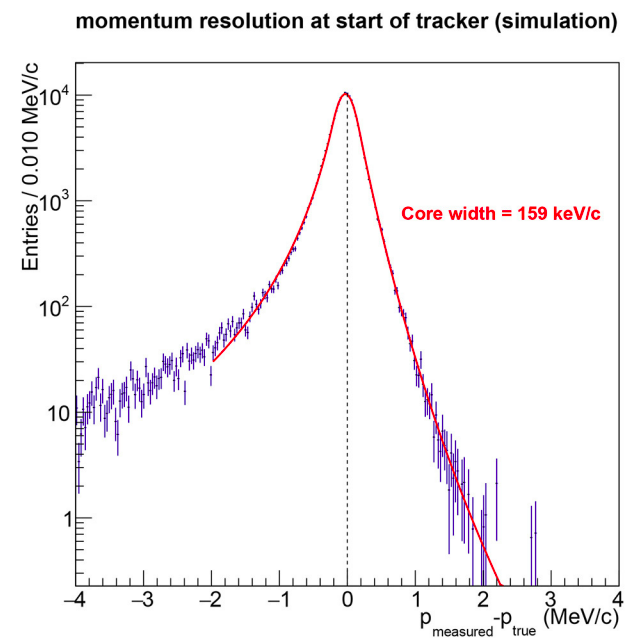
\includegraphics[width =0.5\textwidth]{figures/png/Screenshot_20240330_104830.png}
    \caption[The momentum resolution of the straw tracker.]{Momentum resolution of the straw tracker as determined for 
    a sample of Monte Carlo CEs \cite{bobbb}.}
    \label{fig:trkres}
    \end{figure} 
To minimise the probability of scattering and the energy loss of the CE, 
the volume inside the DS is evacuated to $10^{-4}$ Torr. 
The Mu2e collaboration has selected the straw-tube 
technology \cite{bobbb} for its tracker, driven by the need for 
a detector with high core resolution, minimal high-side tails, 
and low energy loss. This choice led to straw tubes, which 
offer a combination of low mass, rapid drift times, good spatial 
resolution and they are in wide use in particle physics. 

The detector has an annular shape with an active region covered by straws only between the 
internal radius of 380 mm and the external radius of 700 mm.  

Chapter \ref{chaptertrk} will provide a more detailed description of the entire detector, 
including the mechanical structure, the FEE and 
DAQ system.
\subsubsection{Momentum scale calibration}
One of the most challenging aspects of the Mu2e experiment is achieving the 
required momentum resolution to distinguish the CE electron from the background.

Mu2e requires at least one source of high-energy calibration electrons or 
positrons to independently measure the absolute momentum scale of the tracker. 
The momentum scale calibration relies on accurately reconstructing the 
$\pi^+ \rightarrow e^+ \nu_e$ peak ($BR\sim 1.23 \times 10^{-4}$), with its success critically dependent on the 
suppression of $\mu^+ \rightarrow e^+ \nu_e \bar{\nu}_\mu$ decays in flight (DIF). 
Several approaches have been explored, with the most promising ones being:

\begin{enumerate}
    \item Special run with adjusted TS collimators: operating with 
    reversed TS collimators and a reduced DS field 
    (70\% of the nominal value), this setup is designed to capture the 
    leptonic decay ($\pi^+ \rightarrow e^+ \nu_e$) of stopping $\pi^+$ in the nominal ST;
    
    \item Low intensity run with reduced DS magnetic field: 
    running at low intensity and a further reduced DS field 
    (50\% of the nominal value), 
    this approach aims to gather high-statistics data to accurately fit 
    the Michel edge of the DIO momentum distribution.
\end{enumerate}

Several important considerations include:

\begin{itemize}
    \item Early time measurement: to reconstruct the $\pi^+ \rightarrow e^+ \nu_e$ decays, 
    measurements must be performed at early times, approximately 
    $T \sim 300$ ns. This necessitates operating at a reduced proton 
    beam intensity to mitigate the pileup;
    
    \item Special instrumentation requirement: to minimize 
      the background from muon decays in flight, a beam degrader
      in the DS is needed.
\end{itemize}

The momentum scale calibration described involves two key measurements: 
\begin{enumerate}
    \item The edge of the positron momentum spectrum 
    from $\mu^+ \rightarrow e^+ \nu_e \bar{\nu}_\mu$ decays 
    at $B = 0.5$ T;
    \item The $\pi^+ \rightarrow e^+ \nu_e$ peak at $B = 0.7$ T.
\end{enumerate}

Each of these measurements determines the momentum scale at their respective 
magnetic field values. By combining these measurements, we can extrapolate the 
momentum scale to the nominal magnetic field, $B = 1.0$ T. This concept is illustrated in Figure \ref{fig:momscale}.

\begin{figure}[!h]
\centering
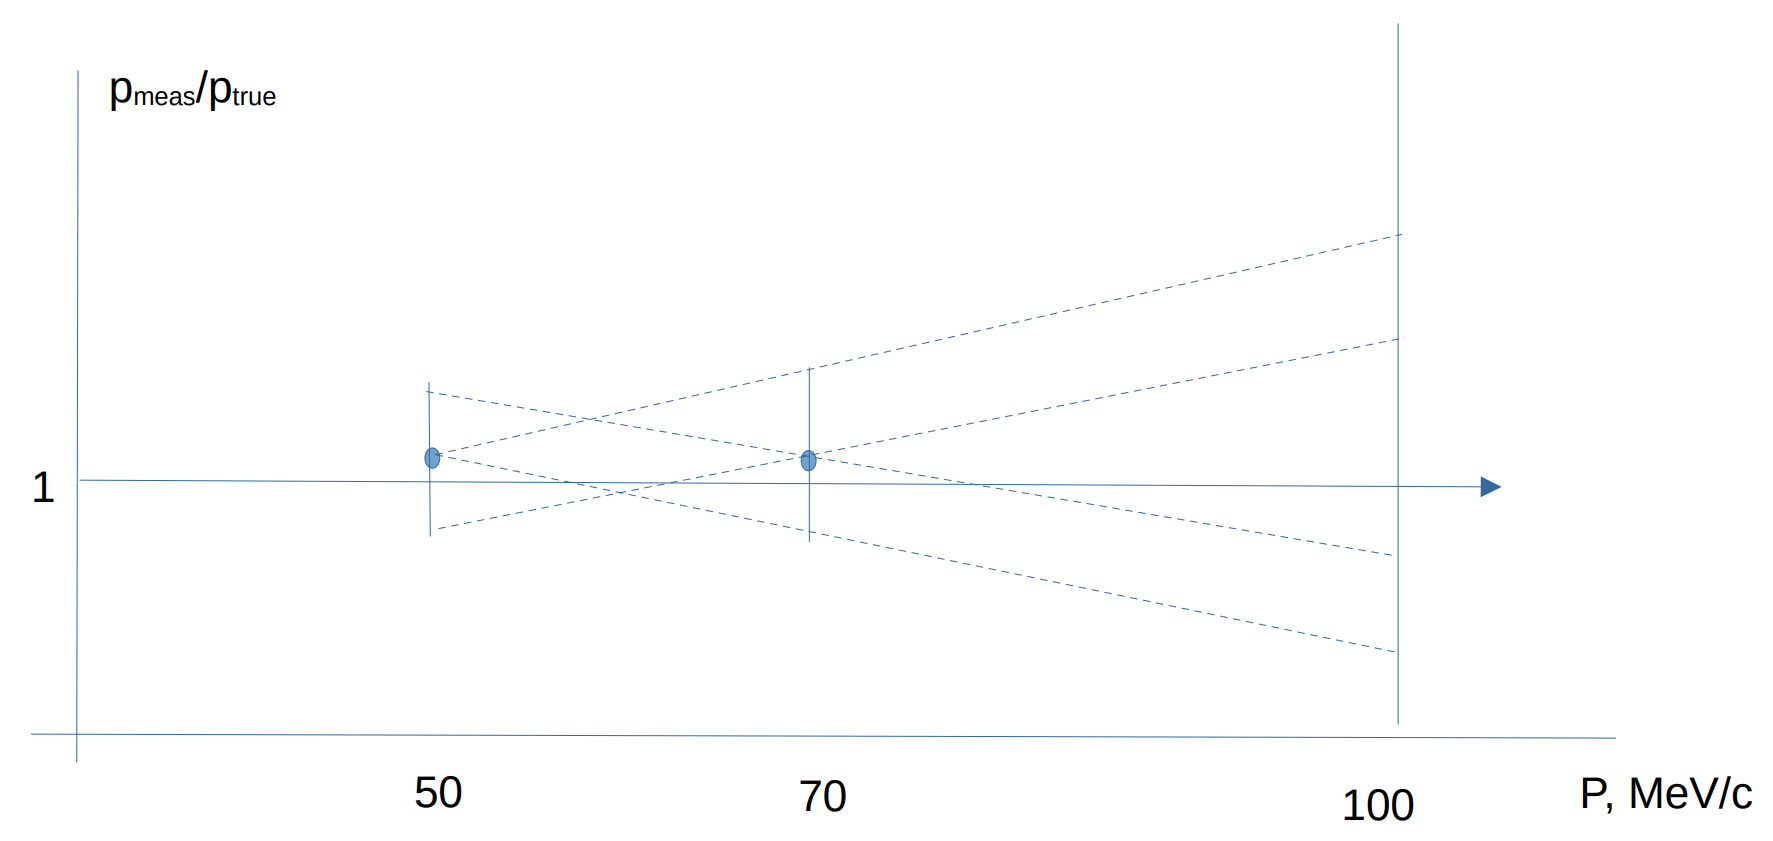
\includegraphics[width=0.7\textwidth]{figures/png/Screenshot_20240909_140555.png}
\caption[The momentum calibration scheme.]{Illustration of the momentum calibration scheme.}
\label{fig:momscale}
\end{figure}

The calibration scheme assumes that the magnetic field is initially set based 
on readings from an NMR probe.

\subsection{The electromagnetic calorimeter}\label{calorimeter}
The Mu2e electromagnetic calorimeter serves multiple purposes \cite{em4}:
\begin{itemize}
    \item the measurement of the energy deposited in the calorimeter 
    allows to separate electrons and muons of the same momentum. 
    The energy-to-momentum ratio ($E/p$) will be used for particle 
    identification and to suppress the background due to cosmic muons;
  \item the calorimeter information 
    helps improving the pattern recognition and 
    the quality of the track reconstruction;
    \item it provides independent triggers from the track-based triggers \cite{em6}. 
\end{itemize} 
For these purposes, the calorimeter needs to fulfill the following physical requirements:
\begin{itemize}
    \item an energy resolution better than $\sigma_E/E \sim$10\% allows
     to reach a rejection factor at the level of 200 between CE
    and the $\sim$ 40 MeV energy deposit from 105 MeV/c cosmic ray muons mimicking the signal;
    \item a timing resolution better than 500 ps ensures that
    the energy depositions in the calorimeter are in time with
    the CEs reconstructed by the tracker and
    also improves the PID;
    \item a position resolution of $\sim$6 mm allows 
    to match the position of the energy deposit with the 
    extrapolated trajectory of a reconstructed track;
    \item it should perform a fast enough 
      response in order to handle the experimental high rate ($\tau < 40$ ns);
    \item a temperature and gain stability within $\pm$0.5\% 
    are required not to deteriorate the energy resolution;
    \item it must be capable of operating in 
    a magnetic field of 1 T, a pressure of \(10^{-4}\) torr, a 
    neutron flux equivalent to \(10^{12}\) n/cm\(^2\)/year, 
    and in a high radiation environment (exposures up to 15 krad/year);
    \item reliability and redundancy are needed to operate in vacuum for one
    year without any interruptions.
\end{itemize}


The calorimeter disks are being assembled at Fermilab's SiDet facility, as shown in Figure 
\ref{fig:calostatus}. The components will be described in the next sections.

\begin{figure}[!h]
    \centering
    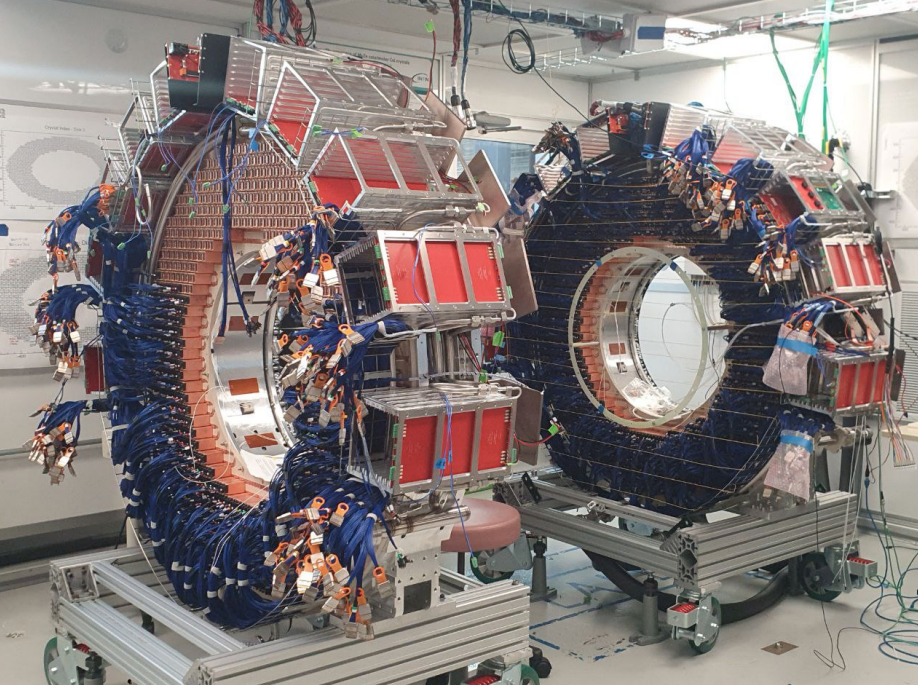
\includegraphics[width =0.6\textwidth]{figures/png/Screenshot_20240706_151533.png}
    \caption[The Mu2e calorimeter disks.]{Mu2e calorimeter disks being assembled at the Fermilab SiDet facility.}
    \label{fig:calostatus}
\end{figure}

\subsubsection{The calorimeter mechanical structure}
The calorimeter is located in the DS downstream of the tracker (Figure \ref{fig:DS})
It consists of two annular disks, with an internal radius of 35 cm and 
an external radius of 66 cm, located at a relative distance of 70 cm (Figure \ref{fig:calo1}).
The separation was chosen to match half of the distance between two periods of the helical trajectory 
of a typical 105 MeV CE. This maximises the detection probability of CEs: electrons which pass through the hole of the first disk will be detector by the second one \cite{em7}. 


The calorimeter mechanical structure was designed to support the layout of the crystals 
by piling them up in a self-standing array organized in consecutive staggered rows. 
Each crystal array is supported by two coaxial cylinders. The inner cylinder must be 
as thin and light as possible in order to minimize the passive material in the 
region where spiraling background electrons are concentrated. The outer cylinder 
is as robust as required to support the load of the crystals (700 kg). Each disk 
has two cover plates. The plate facing the beam is made of carbon fiber to minimize 
the degradation of the electron energy, while the back plate should also be robust 
to support the SiPMs, the FEE and the SiPM cooling lines and it 
is therefore made of Polyether ether ketone (PEEK). The crystal arrangement is 
self-supporting, with the load carried primarily by the outer ring. 
The heat generated by SiPMs, FEE and read out electronics 
must be removed within temperature values acceptable for the correct operation 
of each device. Furthermore, the difficult access to components requires a 
cooling system free of fault and maintenance needs for at least one year. 
The cooling system has to maintain SiPM temperature at approximately -10°C to 
minimize the dark current: this is obtained by circulating a refrigerating fluid at approximately  -15°C.


\begin{figure}[!h]
    \centering
    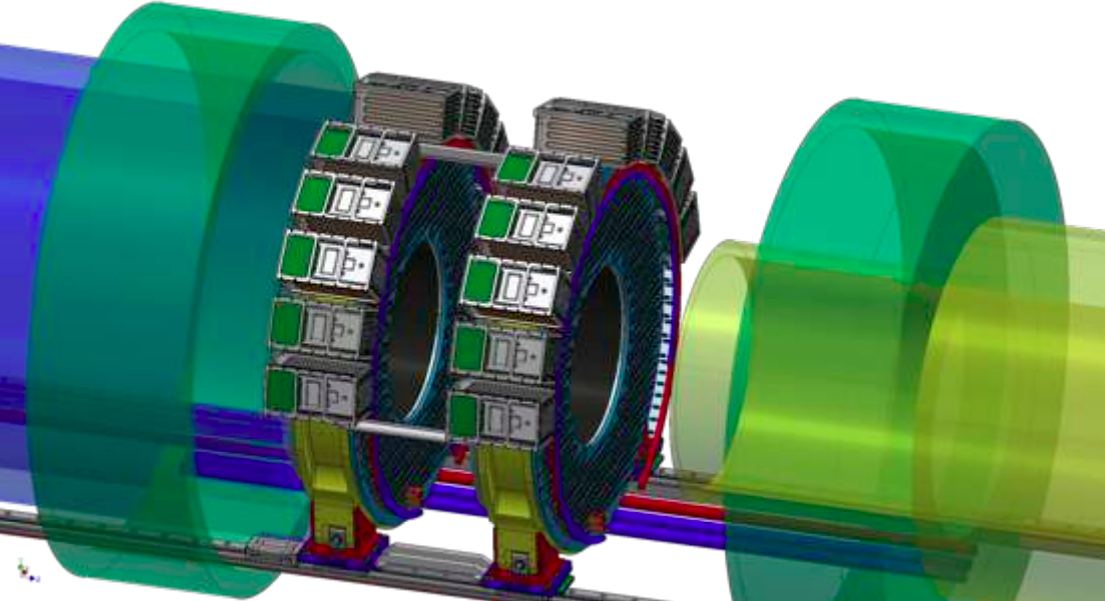
\includegraphics[width =0.6\textwidth]{figures/png/Screenshot_20240322_122050.png}
    \caption[CAD representation of the calorimeter disks.]{Calorimeter disks installed in the Mu2e experimental area (CAD representation) \cite{em7}.}
    \label{fig:calo1}
\end{figure}



\subsubsection{The undoped Cesium Iodide crystals}
Each calorimeter disk is filled with 674 undoped cesium 
iodide (CsI) crystals \cite{em6}, wrapped in a 150 $\mu$m Tyvek foil. 
Undoped CsI represents the best compromise between cost, 
reliability, performance and radiation hardness, providing 
a fast emission time and a sufficiently high light yield. Pure 
CsI has a wavelength peak emission at 310 nm, a scintillation 
time of 20 ns, and a light yield of about 2000 photons/MeV. 
Figure \ref{fig:calo2} (top right) shows some CsI crystals: 
the dimensions are 34$\times$34 200 mm$^3$. The crystal length 
is approximately 10$X_0$ which is sufficient to contain the 105 
MeV CE shower since the average incident angle 
is 50°. Undoped CsI crystals also have the radiation hardness 
adequate for the Mu2e operational conditions. 




\begin{figure}[!h]
    \centering
    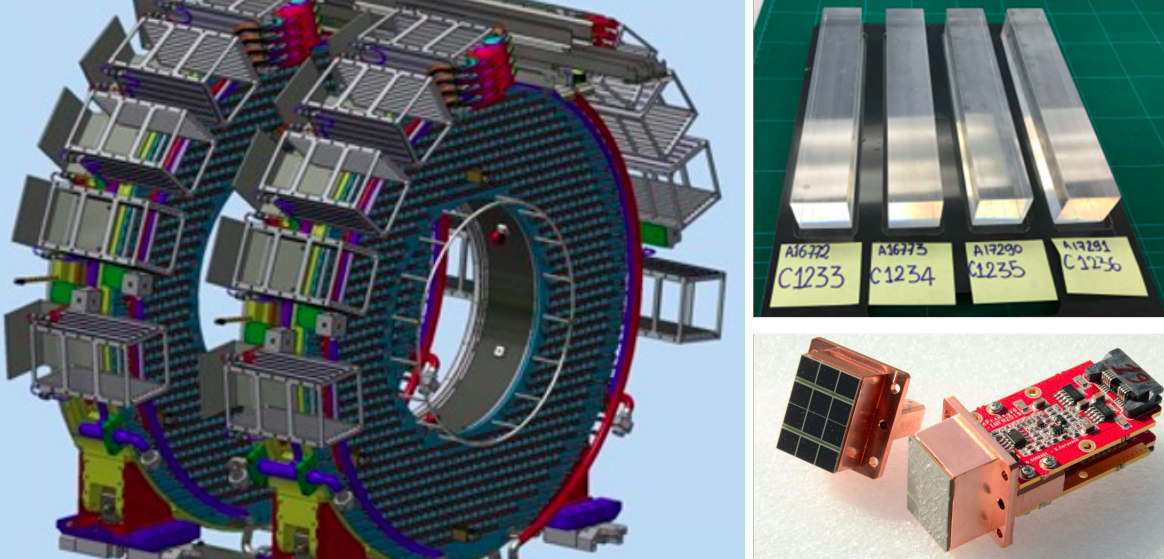
\includegraphics[width =0.7\textwidth]{figures/png/Screenshot_20240322_121000.png}
    \caption[The calorimeter components.]{(Left): Schematic CAD representation of the two calorimeter disks. (Top right): 
    cesium iodided crystal used in the calorimeter. (Botto, right): Two SiPM arrays 
    glued onto the copper holder (left) and one fully assembled readout unit made of two 
    SiPM arrays and two Front-End boards mounted on the copper holder (right) \cite{em4}.}
    \label{fig:calo2}
\end{figure}


\subsubsection{The calorimeter readout chain}
The readout of the calorimeter is performed through a chain of components: Silicon PhotoMultipliers (SiPM), 
FEE, Mezzanine board and Digitizer board. In the following, 
a brief description of each component will be provided.
\paragraph{Silicon PhotoMultipliers (SiPM)}
Since the calorimeter will operate in a 1 T magnetic field, SiPMs were chosen over PMTs (Figure \ref{fig:sipmcell}) \cite{em1}. 
To well match the scintillation emission of 310 nm to the SiPM photon detection efficiency, 
UV extended Hamamatsu SiPMs with a front window made of a silicon resin were selected. Each SiPM is composed of a
2 $\times$ 3 array array of individual 6 mm $\times$ 6 mm cells.
The array can be seen as the parallel of two series of 3 cells, that 
are powered by the same source. The mixed configuration is motivated by 
two competing requirements: a parallel connection has greater capacitance and a higher response time 
but requiring a lower bias voltage, whereas 
a series connection has the opposite characteristics. 
To improve reliability, light collection efficiency and resolution, each single 
crystal is readout by two custom SiPMs arrays.
Magnetic field resistance was the factor in choosing between SiPMs and PMTs.
The good efficiency of the SiPMs allows to collect approximately 20 p.e./MeV per SiPM.
To operate in vacuum, minimise outgassing contributions, reduce 
thermal coupling between crystals and FEE, the crystal-SiPM 
coupling is done without any optical grease and a 2 mm air gap is mantained 
between the crystal and the readout sensor.

Since the main scintillation component has a wavelength of 315 nm to match the SiPM
photon detection efficiency as a function of wavelength, each crystal is coupled with a readout 
module consisting of two ultraviolet (UV)-extended SiPM arrays
and the corresponding analog FEE boards, as illustrated in Figure 
\ref{fig:calo2} (bottom right) \cite{em5}, \cite{em2} and \cite{em3}. 
As shown in Figure \ref{fig:calo3}, each board is positioned within the electronic 
crates that surround the calorimeter disks.
\begin{figure}[!h]
        \centering
        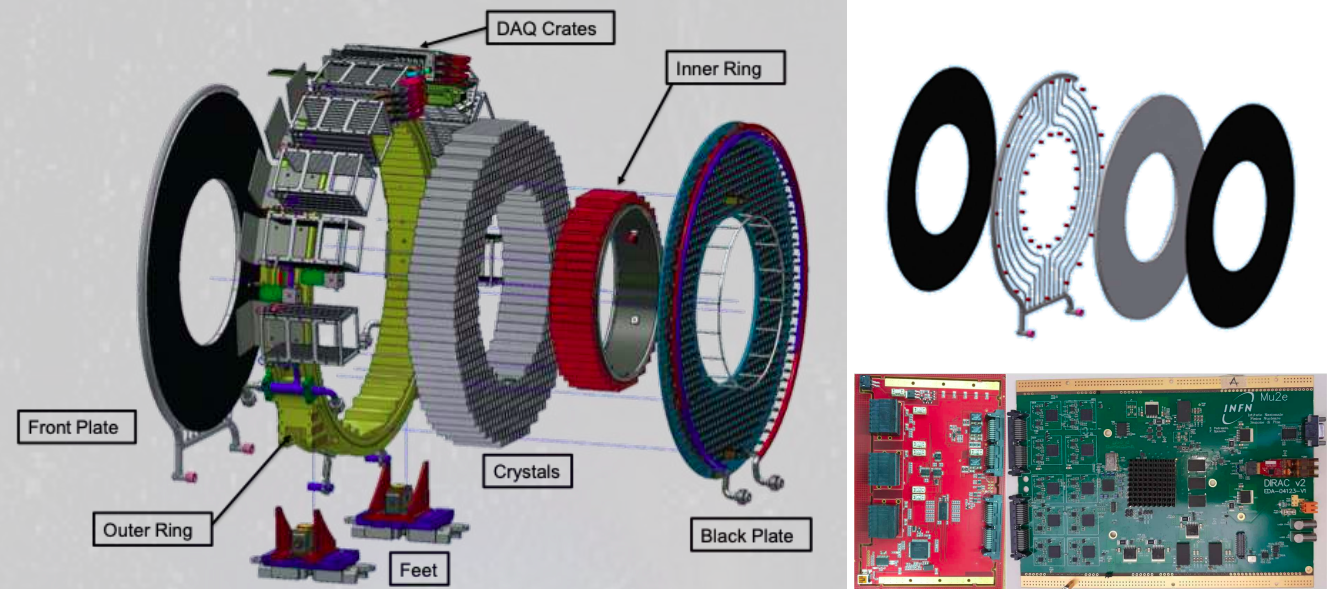
\includegraphics[width =0.8\textwidth]{figures/png/Screenshot_20240322_121017.png}
        \caption[The breakout of calorimeter mechanical components.]{Left: the breakout of calorimeter mechanical components. Top right: the breakdown of front
        panel plate. Bottom right: the Mezzanine and DiRAC boards \cite{em4}.}
        \label{fig:calo3}
        \end{figure}


\begin{figure}[!h]
    \centering
    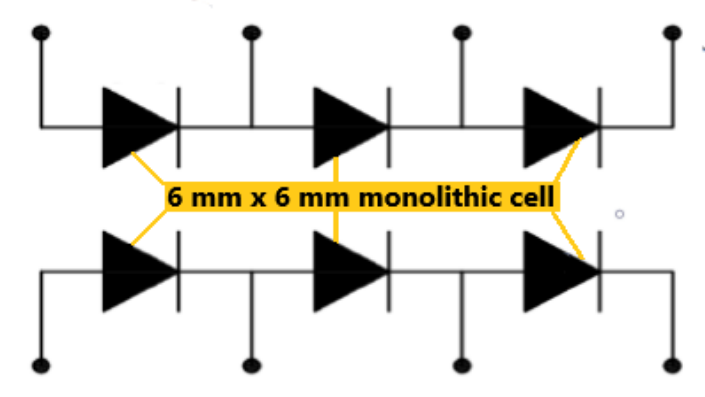
\includegraphics[width =0.6\textwidth]{figures/png/Screenshot_20240706_141625.png}
    \caption[The design of SiPM cells.]{The design of a 2$\times$3 array of SiPM cells.}
    \label{fig:sipmcell}
\end{figure}
\paragraph{The Front-End electronics}
Each SiPM is read by one Front-End board directly linked to the pins on the 
back of the SiPMs and, via cable, to the Mezzanine board (Figure \ref{fig:connectiontomezzanine}). 
The Front-End board provides signal preamplification and shaping, local linear 
regulation of the SiPM bias voltage, and monitoring of the SiPM current and temperature. 
The two Front-End boards connected to the two SiPMs reading the same CsI 
crystal are housed in a copper holder (Figure \ref{fig:holder}), which 
serves as a mechanical support and ensures SiPM cooling. 
An enternal Faraday cage reduces the noise. The holder also holds 
an optical fiber used to pulse the crystal with a laser light to 
calibrate the energy and time response.
\begin{figure}[!h]
    \centering
    \begin{subfigure}[t]{0.5\textwidth}
        \centering
        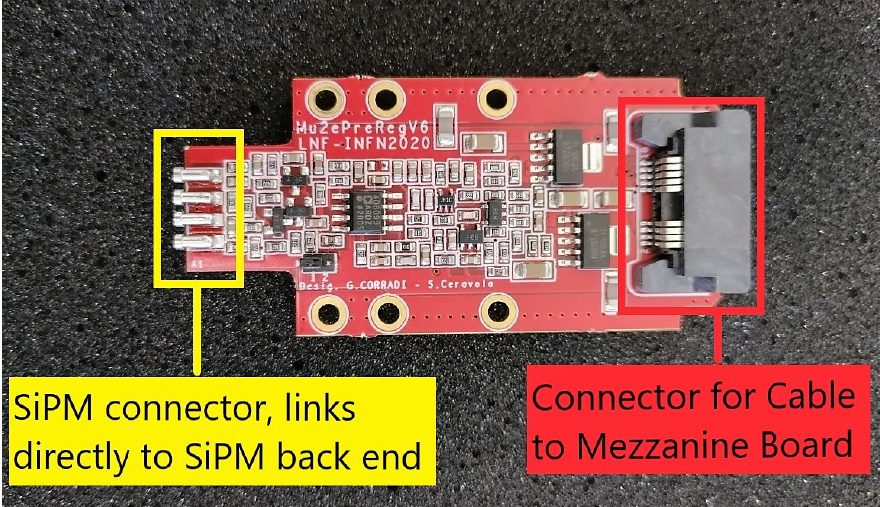
\includegraphics[width=0.85\textwidth]{figures/png/Screenshot_20240706_143204.png}
        \caption{}
        \label{fig:connectiontomezzanine}
    \end{subfigure}%
    ~ 
    \begin{subfigure}[t]{0.5\textwidth}
        \centering
        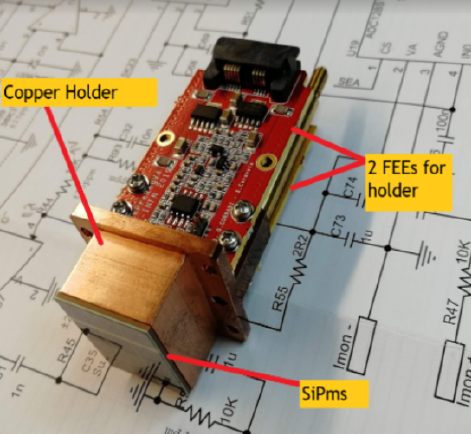
\includegraphics[width=0.85\textwidth]{figures/png/Screenshot_20240706_143517.png}
        \caption{}
        \label{fig:holder}
    \end{subfigure}
   \caption[The calorimeter FEE board.]{(a): The FEE board, with its connectors to SiPMs 
   back and to the cable coming from Mezzanine. 
   (b): The assembled FEE holder.}
    \label{fig:calooo}
  \end{figure}


\paragraph{The Mezzanine board}
The Mezzanine Board serves as the interface between 20 different 
Front-End boards and one Digitizer (Figure \ref{fig:mezzanine}) 
The Mezzanine sets all FEE parameters (such as High Voltage (HV)) and 
monitors all Front-End boards and SiPM parameters (such as HV, temperature, and current). 
It also provides low voltage to the Front-End boards. The HV of each SiPM can be 
independently set. These tasks are performed by an ARM processor located on the 
Mezzanine board. The cables chosen to link the Front-End boards to the 
Mezzanine board must be radiation-resistant, shielded, and have low outgassing. 
\begin{figure}[!h]
    \centering
    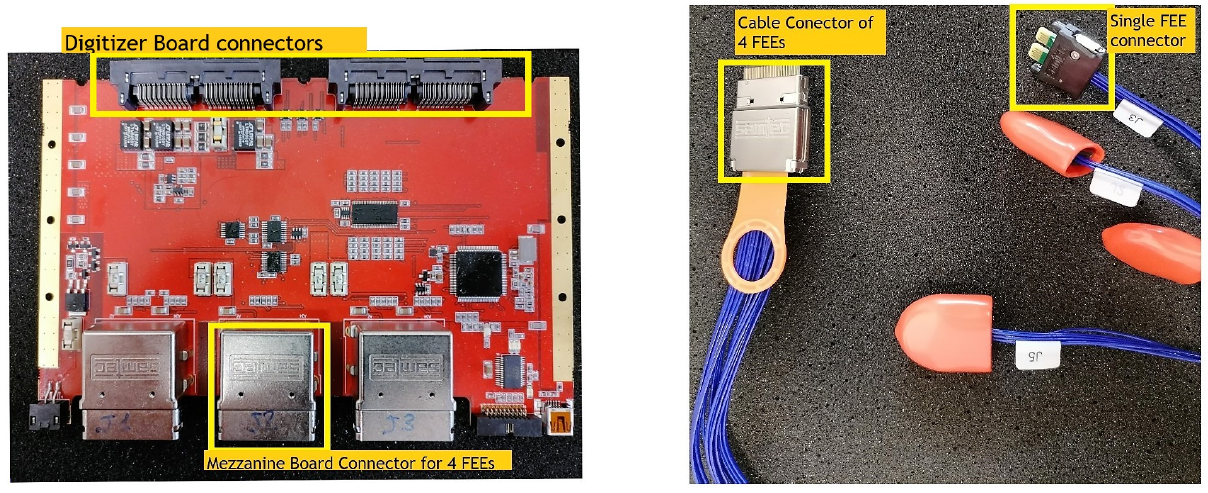
\includegraphics[width =0.8\textwidth]{figures/png/Screenshot_20240706_144234.png}
    \caption[The calorimeter Mezzanine Board and FEE.]{Left: The Mezzanine Board with connectors highlighted. 
    Right: The Cable linking 4 FEEs to one Mezzanine.}
    \label{fig:mezzanine}
\end{figure}



\paragraph{The digitizer Board}
The Digitizer Readout Controller (DiRAC) digitizes the SiPM 
signals received from the Mezzanine Board and manages data 
transmission to the experiment's DAQ system. Zero suppressed 
data are sent from the DiRAC board to the DAQ via optical fibers. 
A sampling rate of 200 MHz (one sample every 5 ns) and a 12-bit resolution 
satisfy the calorimeter requirements. The two SiPMs which read the same 
crystal are always connected to different DiRAC boards hosted in separate 
crates to prevent a complete loss of a crystal 
in an event of a single crate fault.

\paragraph{The crate}
The Mezzanine and DiRAC boards reside in crates.
Each crate contains up to eight Mezzanine 
and DiRAC boards and provides cooling to the boards via a network of cooling lines grooved in the crate walls.
The thermal contact between the electronics components on the Mezzanine and the DIRAC
and the crate walls is ensured by a copper plate covering the entire board.
\subsubsection{Module-0 prototype}
To validate the chosen design before commencing the mass production of 
the calorimeter components, a large-scale prototype was constructed and 
tested with an electron beam at the Beam Test Facility of the National 
Laboratories of Frascati. The Module-0 consists of 52 undoped CsI crystals, 
read by 102 SiPMs connected to FEE boards. Its mechanics was designed

to closely resemble the final calorimeter, allowing for the testing 
of the assembly procedures and cooling.
The energy and time resolution are
shown in Figure \ref{fig:calores} \cite{bobbb} and \cite{calo95}.
\begin{figure}[!h]
    \centering
    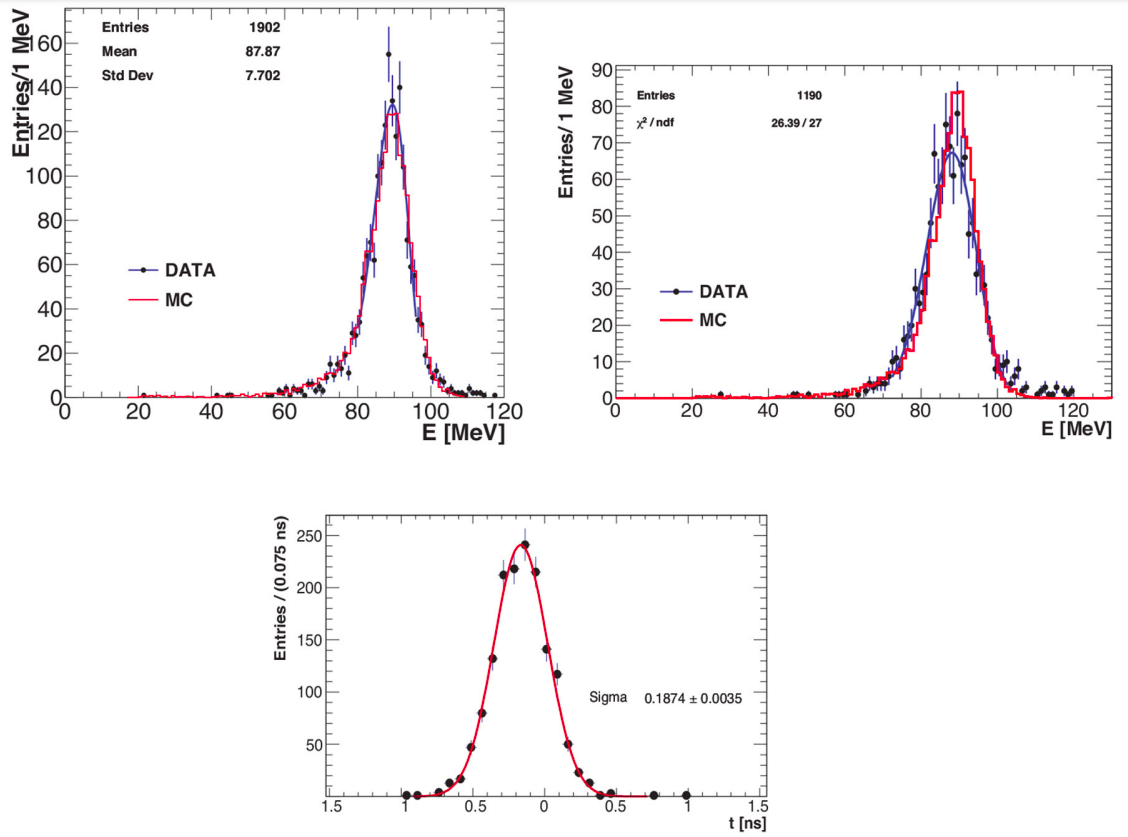
\includegraphics[width =0.8\textwidth]{figures/png/Screenshot_20240330_105520.png}
    \caption[The energy and time resolution of the calorimeter Module-0.]{The 
    energy and time resolution of the Module-0 for the Mu2e 
    calorimeter for electrons at the conversion energy. (Top left) The resolution 
    for electrons striking the array at normal incidence. (Top right) 
    Resolution for electrons striking the array at 50° with respect to the 
    face. (Bottom) The time resolution. All measurements are compared with 
    simulations (red line) \cite{bobbb} and \cite{calo95}.}
    \label{fig:calores}
\end{figure}
\subsection{The Cosmic Ray Veto}\label{CRV}
As reported in the Section \ref{backgrounds}, the expected Mu2e 
cosmic background is at a level of 1 signal-like event per day. 
To minimize the backgrounds, Mu2e exploits a combination of passive shielding and an active 
veto system named CRV. Figure \ref{fig:crv} shows a 
schematic representation of 
the CRV covering the region of the DS and half of the Transport Solenoid 
almost entirely (there is no veto on the floor at the bottom), for a total detector area
of 327 m$^2$.
The CRV modules are manufactured from plastic scintillator extrusions. 
In different regions of the detector the extrusions may have different lenghts, 
but they all have the same cross-sectional area of $5 \times 2$ cm$^2$.
The extrusions 
are coated with Titanium dioxide to improve internal reflections and thus, the light yield. 
Two grooves are extruded inside the scintillator bar throughout its length to contain two 
1.4 mm diameter wavelength shifting fibers. The fibers transport light to the extrusion 
ends where each fiber is instrumented with a $2 \times 2$ mm$^2$ SiPM at each end. Figure \ref{fig:crvmodule} 
shows the cross-section of a CRV module. Each module is made of four overlapping staggered layers 
of plastic scintillator counters to reduce the effects of gaps. The 
layers are separated by 10 mm aluminium plates used as absorbers. 
When three of the four layers of the CRV are activated, an offline veto window is opened.
A conversion-like event observed during this time window is assumed to be produced by a cosmic-ray muon
and will be disregarded. 
The estimated total dead time is $\sim$5\%.
Based on the simulation, the required CRV veto efficiency is 99.99\% within the detector fiducial.

\begin{figure}[!h]
\centering
\includegraphics[width =0.65\textwidth]{figures/jpg/Crv_downstream.jpg}
\caption[The CRV features and components.]{The CRV covers the DS entirely and half 
of the Transport Solenoid. It is made of several sectors, including the top 
(CRV-T), the right (CRV-R), the left (CRV-L), the upstream (CRV-U), the downstream 
(CRV-D), and the hole where the Transport Solenoid enters the enclosure (TS-hole) \cite{bartoszek2015mu2e}.}
\label{fig:crv}
\end{figure}

\begin{figure}[!h]
\centering
\includegraphics[width =0.65\textwidth]{figures/png/Crv_module_geometry.png}
\caption[The cross-section of a CRV module.]{Cross-section of a CRV module, including geometry and nomenclature. 
There are internal gaps between counters in a di-counter \cite{Giovannella_2020}.}
\label{fig:crvmodule}
\end{figure}
\subsection{The Muon Beam Stop and the Stopping Target Monitor}
A Muon Beam Stop (MBS) is installed at the downstream end of the DS to 
absorb muons that are not stopped in the ST, shown in Figure \ref{fig:stm}. 
The MBS has been designed to limit the effects of muon decays and captures. 
The magnetic field gradient prevents the majority of the low-energy charged 
particles created in the MBS from moving upstream towards the detectors.  
The MBS is made of high-$Z$ minerals and polyethylene. Muons have an extremely short lifetime in 
high-$Z$ materials, as shown in Figure \ref{fig:muonicatom}, which minimizes the effects of muon 
decays and captures much earlier than the Mu2e live window starting at 640 ns. Moreover, polyethylene 
absorbs protons and neutrons emitted by the excited nuclei during muon captures.  

The STM is placed downstream from the MBS, as shown in Figure \ref{fig:stm}, 
to measure the number of muons stopped on the ST.

\begin{figure}[!h]
    \centering
    \includegraphics[width =0.7\textwidth]{figures/png/Screenshot_20240306_180910.png}
    \caption[The Stopping Target Monitor geometry.]{The STM geometry showing the DS region (left), 
    the End Cap Shielding, sweeper magnet and STM field-of-view collimator. 
    At the far end of the hall (right) is the final $spot-size$ collimator and the STM detector.}
    \label{fig:stm}
    \end{figure}
    The STM measurement technique exploits the 347 keV X-ray line produced in the 2p$\rightarrow$1s 
    radiative transition of the muon moving to the ground state in the muonic atom (Figure \ref{fig:stmprocess}), 
    which is present for 80\% of the stopped muons. Although the 2p$\rightarrow$1s transition has the 
    largest yield, there are also additional X-ray transitions with substantial yields, 
    including 3p$\rightarrow$1s and 4p$\rightarrow$1s. In addition, the 3d$\rightarrow$2p 
    transition that populates the 2p state appears in the energy spectrum.

    An alternative option is to measure gamma rays associated 
    to muons interactions in the ST (Figure \ref{fig:stmprocess}).
    These are unambiguous signals that muons stopped in the aluminum target. 
    The main signatures are the following ones: 
    \begin{itemize}
    \item 1809 keV gamma-ray that is emitted in the nuclear capture chain:
    \begin{equation}
        \mu^- \ + \ ^{27}\text{Al} \ \rightarrow \ ^{26}\text{Mg}^* \ + \ \nu_\mu \quad \quad ^{26}\text{Mg}^* \ \rightarrow ^{26}\text{Mg} \ + \ \gamma(1809 \ \text{keV})
     \end{equation}
     The $^{26}\text{Mg}^*$ mean de-excitation time is negligible (476 fs) with 
     respect to the muonic atom lifetime (864 ns). 
     This process occurs for 51\% of the nuclear captures.
     \item  A 844 KeV gamma-ray coming from the decay of 
       long-lived ($\tau \sim$9.5 min) isotopes produced in muon nuclear captures:       
     \begin{equation}
        ^{27}\text{Mg} \ \rightarrow \ ^{27}\text{Al} \ + \ \gamma(844 \ \text{keV}) \ + \ e^- \ + \ \bar{\nu}_e
     \end{equation}
     This process occurs for the 9.2\% of nuclear captures.
\end{itemize}

\begin{figure}[!h]
    \centering
    \includegraphics[width =0.6\textwidth]{figures/png/Screenshot_20240706_094517.png}
    \caption[The muon stops 
    and nuclear captures detection in Al ST.]{Reactions that can be exploited to detect the muon stops 
    and nuclear captures in the Aluminum ST.}
    \label{fig:stmprocess}
    \end{figure}

    The Mu2e STM has been designed to determine the number of 
    muons in the ST within 10\% precision over the course of the experiment.  
    It is made of two solid state High Purity Germanium (HPGe) crystal detectors and one 
    scintillating lanthanum bromide (LaBr$_3$) detectors. The HPGe detectors have the 
    energy resolution (FWHM) of 2.5 keV in the energy range of 300-2000 keV and are used 
    to measure photons produced by the secondary muonic aluminium orbital transitions 
    (347 keV) and nuclear captures (884 keV). The LaBr$_3$ detector has an order of 
    magnitude worse energy resolution than the HPGe detector, but it provides a much 
    higher rate capability. It is used to detect prompt photons produced
    in the nuclear captures (1809 keV).  
    \begin{figure}[!h]
        \centering
        \includegraphics[width =0.4\textwidth]{figures/png/Setup.png}
        \caption[The Stopping Target Monitor geometry.]{The STM geometry.}
        \label{fig:stmfigure}
        \end{figure}
The STM geometry is shown in Figure \ref{fig:stmfigure}.





\chapter{The Mu2e tracker}\label{chaptertrk}

\textit{The following Chapter will focus on the Mu2e tracker, one of the most important detectors in Mu2e. 
It will give further information about the straw tube tracker panels, 
including the detection mechanism, the mechanical design and the Front End Electronics (FEE).
As previously pointed out, the Mu2e tracker is made up of 216 identical panels. 
Each panel is a mechanical and electrical standalone module. Each panel has 96 drift 
tubes used as fundamental detecting components. I will start by discussing the 
theoretical characteristics of drift tubes and then I will go more in detail with Mu2e tracker features. 
Most of the discussion is based on \cite{kola} and \cite{bobbb}.}

\section{Drift Tubes}
Gas detectors are capable of measuring charged particle coordinates. 
They provide great spatial resolution and detection efficiency at a low cost, Ref. \cite{kola}. 
There are many different gas ionizazion detectors, one of these is the drift tube.
The basic configuration of a drift tube is shown in Figure \ref{fig:drifttube}.
The cylindrical conducting tube, the cathode, is grounded.
A hollow cylindrical conducting tube is grounded and serves as the cathode.
The tube is filled with a combination of noble gas, often Argon, and quench gas. 
A thin sensing wire is suspended along the cylindrical cathode axis. 
The wire, called anode, receives a high voltage. Long and thin drift tubes, known as $straw$ $tubes$, have a similar form.
\begin{figure}[!h]
    \centering
    \includegraphics[width =0.8\textwidth]{figures/png/Screenshot_20240324_232621.png}
    \caption{Schematics of a drift tube, Ref. \cite{kola}.}
    \label{fig:drifttube}
    \end{figure}
Assuming an anode radius $a$, a cathode radius $b$ and using Gauss theorem, the electric field is:
\begin{equation}\label{avalanche}
    E(r)=\frac{1}{r}\frac{\lambda}{2\pi \epsilon}=\frac{1}{r}\frac{V}{ \text{ln}(b/a)} \qquad (a<r<b)
\end{equation}
Where $\lambda$ is linear charge density on the wire and $\epsilon$ is the dielectric constant of the gas.
Thinner wires are typically preferred in drift tubes. A greater electric field near the wire increases the amplification factor 
of the drift tube at the same voltage. Additionally, smaller wires improve spatial resolution, Ref. \cite{kola}. 
\subsection{Gas Ionization}
Two are the interactions that can deposit energy when particles traverse the gas volume: ionization and excitation.
Collisions between a charged particle $C$ and an atom $A$ can result in the ejection of one or more electrons: 
$A \ C \rightarrow A^+ e^- C$, or $A \ C \rightarrow A^{++} e^- e^- C$, if more than one electron is released.
This process is called primary ionisation. The mean energy loss per path length can be determined using the Bethe-Bloch formula.
A noble gas atom $A$ can turn also into an excited state $A^*$ through the interaction $A \ C \rightarrow A^* C$. 
If the excitation energy of $A^*$ is higher than the ionization potential of another species $B$ in the gas, the quencher, the
Penning Effect can produce ionization through $A^*B \rightarrow A B^+ e^-$. In addition, the noble gases can
also form molecular ions through processes such as $A^* A \rightarrow A_{2}^{*} \rightarrow A^+_2 e^-$.
A secondary ionisation can occurr through these processes or through electrons that have sufficient energy for generating more ions.
To compute the average number of electron-ion pairs produced by an initial particle, divide its total energy loss 
by the average energy required to make an electron-ion pair. Due to the energy lost during excitation, this average 
does not match the gas ionisation potential. Measurements showed an average of one electron-ion pair every 
30 eV, with variations depending on gas composition and starting particle. Except for very slow particles, 
this value remains constant regardless of their initial energy.
Without an electric field, electrons and ions created during ionisations spread uniformly. 
Collisions cause them to lose energy and eventually reach thermal equilibrium with the surrounding gas. 
They eventually recombine. An electron maximal range during ionisation is correlated with its initial kinetic 
energy. In a normal temperature and pressure gas, a 10 keV electron may be stopped in approximately 1 mm. 
Ionised electrons often have reduced kinetic energy, leading to a shorter range.
\subsection{Drift of Ions and Electrons}
The electric field accelerates free electrons and ions towards the anode and cathode 
along the field lines. As charges accelerate, they scatter on other particles in the gas, 
losing energy. The directions of motion are randomised, and maximum speeds are set. As a result, 
charges move uniformly along the electric field. This is referred to as the drift velocity of the 
charge. It is superimposed with the thermal motions.
Drift velocities for ions and electrons varies based on several parameters. Ions have a bigger mass 
than electrons and their masses are comparable to those of gas molecules. During collisions, gas 
molecules absorb a significant portion of the energy gained from ions during acceleration. In a drift 
tube detector just a little amount of electric field energy enters the energy associated with ion motion, 
making it comparable to the initial thermal energy before acceleration. 
The ion drift velocity $v_i$ is proportional to the reduced electric field $E/N$ where N is the number density of the gas 
and it is typically $\mathcal{O}(10^3)$ cm/ns, except in the region near to the anode wire where a stronger 
electric field is present. The ion thermal velocity is typically $\mathcal{O}(10^4)$ cm/ns at room temperature.
On the opposite, only a small fraction of the energy is released during elastic collision from electrons, 
so they acquire more energy from the electric field than their thermal energy.
Many different factors impact electron drift velocity. Some gas molecules, such as H$_2$O or CO$_2$, 
can interact with electrons to produce negative ions due to their great electron affinity. In rare situations, 
electrons gather enough energy to exceed gas molecule excitation threshold, resulting in inelastic collisions. 
Electron drift velocity is a complex function of electric field intensity due to several variables influencing 
electron collisions across a large energy range. Figure \ref{fig:drift} shows the electron drift
velocity at different electric field strengths in argon-carbon dioxide mixtures (Ar-CO$_2$) of different
proportions, Ref. \cite{ZHAO1994485}.
\begin{figure}[!h]
    \centering
    \includegraphics[width =0.7\textwidth]{figures/png/Screenshot_20240330_102206.png}
    \caption{Electron drift velocity versus electric field in Ar:CO$_2$ mixtures of different proportions, Ref. \cite{ZHAO1994485}. 
    80\%:20\% Ar:CO$_2$ mixture is the gas used in the Mu2e tracker.}
    \label{fig:drift}
\end{figure}
Electron drift velocities in drift tubes are typically $\mathcal{O}(10^6)$ cm/ns.
This is significantly higher than ion drift velocities and comparable to electron thermal velocity under the same conditions. 
The radial coordinate of an ionisation can be computed using the electron drift velocity and time.
Since drifting electrons and ions are scattered on gas molecules, they also diffuse along their trajectory. 
Electrons diffuse significantly quicker than ions because of their high velocity. Electron diffusion limits 
the intrinsic resolution of drift tubes used to measure incoming particle coordinates. CO$_2$ has internal 
degrees of freedom at low collision energies, preventing electron energies from exceeding thermal energy until 
field strengths above about 2 kV/cm. This improves intrinsic spatial resolution.
\subsection{Avalanche Multiplication}
Electrons can ionise when they face a high electric field near the anode wire. 
The released secondary electrons form tertiary electrons, and so on. Free electrons rapidly multiply, 
resulting in an avalanche. In a drift tubes, where the electron mean free path is about the order of $\mu$m, 
an avalanche develops when the electric field approaches $\mathcal{O}(10)$ kV/cm. 
According to Equation \ref{avalanche}, using $a \sim \mathcal{O}(10^{-3})$ cm, $b \sim \mathcal{O}(1)$ cm and
a normal voltage of 1-2 kV, the avalanches can occur within $\mathcal{O}(100) \ \mu$m from the anode wire. 
Electrons from the avalanche are collected on the anode wire within 1 ns, while positively charged ions move towards the cathode.
Drifting ions mostly generate signals in electrodes via induction. Figure \ref{fig:avalanche} shows the model of an ionisation avalanche.
\begin{figure}[!h]
    \centering
    \includegraphics[width =0.7\textwidth]{figures/png/Screenshot_20240330_182509.png}
    \caption{The model of an ionisation avalanche forming at the anode wire of a proportional tube or chamber, Ref. \cite{kola}. 
    (a) In the drift volume, electrons and ions are generated and drift to their corresponding electrodes. 
    (b) Near the wire, the electron achieves a high enough field to induce secondary ionisation, resulting in an avalanche. 
    (c) The electric field separates charges created during an avalanche. 
    (d) Electrons have higher lateral diffusion than ions, causing the avalanche to expand 
    around the wire and produce a positive charge cloud in the shape of a drop. 
    (e) Electrons from the avalanche reach the anode within nanoseconds, but ions take longer, up to ms, to reach the cathode.}
    \label{fig:avalanche}
\end{figure}
\subsubsection{Avalanche Gain}
When an avalanche develops, the amplification factor is around $10^4-10^6$. The number of electrons freed per unit path length is given
by the first Townsend ionization coefficient $\alpha=\sigma_{ion}n=1/\lambda_{ion}$ and this depends on the electric field $E$, 
as a higher electric field corresponds to a higher kinetic energy of the electron, that increases the ionization cross-section.
The increase $dN$ of the number of electron-ion pairs over a path length $ds$ is, Ref. \cite{kola}:
\begin{equation}
    dN=\alpha(E)Nds
\end{equation}
Solving this equation, we can easily obtain the gas amplification $G$:
\begin{equation}\label{av}
    G=\frac{N(s_a)}{N_0}=\text{exp} \left( \int_{s_0}^{s_a} \alpha(E(s)) ds \right)=\text{exp} \left( \int_{E_{min}}^{E(a)} \frac{\alpha(E(s))}{dE/ds} dE \right)
\end{equation}
where $N_0$ corresponds to unamplified electrons in $s=s_0$ and $E_{min}$ corresponds to the minimum energy 
for ionisation to occurr. The energy distribution depends on the electric field which is position dependent. 
Since the free path is inversely proportional to the particle density in the gas, $E_{min}(\rho)=E_{min}(\rho_0)\rho/\rho_0$.
It is reasonable to say that the coefficient is proportional to the field strength, $\alpha= \beta E$, in the low field region. 
Adding this relation with Equation \ref{avalanche} and \ref{av}:
\begin{equation}
     \text{ln}(G)=\beta \ a \ E(a) \ \text{ln}\left( \frac{E(a)}{E_{min}}\right)
\end{equation}
where $\beta$ can be related to $w_i$, that is the energy spent for one ionisation and its value is equal to $e \Delta V$.
As the voltage drop per unit path length is $dV = E(s)ds = (\alpha/\beta)ds$, we obtain $dN=N \beta dV$. Integrating, we can see that
$\beta= \text{ln}(2)/\Delta V$, so the gain in a drift tube is:
\begin{equation}
     \text{ln}(G)=\frac{ \text{ln}(2)}{\Delta V} \ a \ E(a)  \ \text{ln}\left( \frac{E(a)\rho_0}{E_{min}(\rho_0)\rho}\right) \qquad E(a)=\frac{V}{a ln(b/a)}
\end{equation}
which is the Diethorn's formula. 
Gain measurements with variable $\rho$/$\rho_0$, $a$, and $E(a)$ can provide the parameters $E_{min} (\rho_0)$ and $\Delta V$. 
The gas temperature $T$, pressure $P$ and operating voltage $V$ significantly impact the gain of a drift tube with a particular shape and gas mixture. 
\subsubsection{Quench Gas}
To avoid subsequent avalanches, the drift tube gas combination may contain a quench gas, such as CO$_2$, 
methane, or other hydrocarbons. During an avalanche, photons are created by gas deexcitation and electron 
attachment to electronegative species, resulting in negative ions. Photons can generate ionisations 
outside the primary avalanche zone or create free electrons on the cathode surface, resulting in secondary avalanches.
The difficulty arises when the signal created is not proportional to the deposited energy by the original particle 
and is no longer localised to the energy deposition point. Enough intense photons can induce a chain reaction of 
secondary avalanches, leading to a continuous discharge. The use of quench gas prevents subsequent 
avalanches by absorbing ionising photons before they travel far. A tiny quantity of quench gas during normal operation 
can significantly decrease secondary avalanches and breakdowns.
\subsubsection{Operation Modes of Gaseous Ionization Detectors}
In drift tube detectors, the number of electron-ion pairs formed during an avalanche is 
proportional to the starting number of electrons, as shown in the gain computation. To 
operate in a proportional mode, an appropriate voltage is needed to reduce the effects 
of avalanche charges on the electric field. Figure \ref{fig:gaseous} illustrates how a 
gaseous ionisation detector may work in multiple modes based on the operating voltage. Higher operating 
voltage leads to higher charges on the electrodes. Low voltage causes ionisation charges to recombine 
before reaching electrodes, leading to no signal collection. At higher voltages, in ionisation chamber 
region, charges can drift to electrodes, but the electric field is insufficient for avalanches to occur. 
Increasing the operational voltage leads to drift tubes and proportional counters. When the voltage 
becomes high enough, proportionality is lost. When electrons from an avalanche are collected, 
the high density of positive ions near the anode might affect the electric field. 
Electrons in future avalanches that enter the area between the positive ion cloud and the wire face a 
decreased electric field, resulting in lower amplification. The electric field becomes greater in the 
tail of the avalanche, which is far from the wire than the ion cloud. This range of voltage is called region of 
limited proportionality. When the operating voltage reaches high values, 
avalanches create sufficiently energy photons to cause secondary avalanches 
that propagate across the detector, independently from the quench gas. 
This results in detector saturating the output. This way of operating is 
called breakdown mode, commonly known as the Geiger-Muller mode.
\begin{figure}[!h]
    \centering
    \includegraphics[width =0.5\textwidth]{figures/png/Screenshot_20240330_203416.png}
    \caption{The dependence of particle gain on applied voltage in gaseous ionisation detectors. 
    The numbers on the axes are for orders of magnitude only and they depend on the device geometry and gas concentration. 
    Drift tubes operate in the proportional mode, Ref. \cite{kola}.}
    \label{fig:gaseous}
    \end{figure}
\subsection{Signal Creation and Propagation}
Drift tube signals do not originate from avalanche charges. In this case, the anode wire would 
receive the complete signal within a few ns. Signal pulses are created by charges on electrodes 
caused by electron and ion mobility. The Shockley-Ramo theorem, Ref. \cite{kola}, can be 
used to determine the induced charge and current. 
The Shockley-Ramo theorem yields various important results. The total induced charge of a moving charge 
$q$ is determined by the initial and final positions only.  A charge pair induces the same amount of 
charge on an electrode as the charge collected on it. Furthermore, if all electrodes are treated as 
an unity, their weighted potential will be one. 
If one electrode completely encloses the others, the weighted field in the contained region is always zero. 
This means that the total induced current across all electrodes is always zero. The Shockley-Ramo theorem can 
be applied to the drift tube. In an avalanche with $N$ electron-ion pairs, we evaluate the induced current 
signal on the anode wire. The current on the cathode has an additional negative sign. The weighted 
potential and field in the straw depend on the radial coordinate $r$:
\begin{equation}
    \psi_w(r)=\frac{\text{ln}(b/r)}{\text{ln}(b/a)}
\end{equation}
\begin{equation}
    \textbf{E}_w(r)=\frac{1}{\text{ln}(b/a)}\hat{\textbf{r}}
\end{equation}
As previously mentioned, the drift velocity of ions, $u$, is proportional to the electric field intensity $E$. Therefore, $u$ = $mu \ E$. 
Then the ion trajectory fulfils:
\begin{equation}
    u=\frac{dr(t)}{dt}=\frac{\mu V_0}{r(t)\text{ln}(b/a)}
\end{equation}
When ionisation occurs at the anode, the starting condition can be approximated as $r(0) = a$. So, the solution to the given differential equation is:
 \begin{equation}
    r(t)=a \sqrt{1+\frac{t}{t_0}} \qquad t_0=\frac{a^2 \ln (b / a)}{2 \mu V_0}
    \end{equation}
Here, $t_0$ represents the characteristic time, which is generally on the order of 1 ns. 
The time $t$ falls within the range $0 < t < t_{max}$, where $t_{max} = t_0 [(b/a)^2 - 1]$. 
The induced current and charge from the wire are expressed as:
 \begin{equation}
    I_{i o n}^{i n d}(t)=-(e N) E_w(r) \frac{\mathrm{d} r(t)}{\mathrm{d} t}=-\frac{e N}{2 \ln (b / a)} \frac{1}{t+t_0}
    \end{equation}
    \begin{equation}
        Q_{\text {ion }}^{\text {ind }}(t)=\int_0^t I^{\text {ind }}\left(t^{\prime}\right) \mathrm{d} t^{\prime}=-\frac{e N}{2 \ln (b / a)} \ln \left(1+\frac{t}{t_0}\right)
        \end{equation}
The total charge created on the wire by the travelling electrons is:
\begin{equation}
    Q_e^{i n d}=-e N\left[\psi_w(a)-\psi_w\left(r_{a v g}\right)\right]=-e N \frac{\ln \left(r_{a v g} / a\right)}{\ln (b / a)}
    \end{equation}
    where $r_{avg}$ is the average position of ionisations in the avalanche. When compared to the total charge 
    induced $Q^{ind}_{tot}(t_{max}) = -eN$, electron mobility in the avalanche accounts for just 1-2\%. 
    Positive ion drift from the avalanche accounts for the majority of the signal. A signal propagates 
    to both ends of the drift tube from the avalanche location.
    Signals with distinct frequency components can propagate at varying velocities. This causes the signal to disperse.
    When determining the longitudinal coordinate of an avalanche using the signal arrival time difference between straw tube ends, various complications emerge.
%For low-frequency components of the signal (for a meter-long drift tube, this translates to a frequency much less than 300 MHz), 
%a quasi-electrostatic approach is sufficient. The signals seen at tubes ends are influenced by impedances between and on the electrodes. 
%On the other hand, for the high-frequency components of the signal, the tube needs to be treated as a transmission line. 
%The propagation speed of a signal wave with frequency $\omega$ is then $c/\sqrt{\omega}$ $\epsilon$($\omega$), 
%where $c$ is the speed of light and $\epsilon$ is the dielectric constant of the gas. As $\epsilon$ is a function of $\omega$, 
%components of different frequencies propagate at slightly different velocities. This leads to a dispersion (widening) of the signal. It brings some subtleties when using signal arrival time difference between straw tube ends to determine the longitudinal coordinate of an avalanche.
\section{tracker panels}
The Mu2e tracker straw tube arrays use the same detection principles as the gaseous ionisation detectors, Ref. \cite{kola}, 
but it has a significant different design and manufacturing improvements to meet the experiment precise requirements.
\begin{figure}[!h]
    \centering
    \includegraphics[width =0.5\textwidth]{figures/png/Screenshot_20240327_000000.png}
    \caption{A picture of the Mu2e straw tube
    compared to a pencil, Ref. \cite{trk}.}
    \label{fig:trkpencil}
    \end{figure}
    \begin{figure}[!h]
        \centering
        \includegraphics[width =0.5\textwidth]{figures/png/Screenshot_20240327_000131.png}
        \caption{The fully assembled tracker panel with its straws, Ref. \cite{trk}.}
        \label{fig:strawtubes}
        \end{figure}
The straw tubes used in the Mu2e tracker \ref{fig:trkpencil} are 5 mm in diameter and 0.33 - 1.17 m in length, 
Ref. \cite{bartoszek2015mu2e}. The straws are wound with two layers of 6 $\mu$m-thick metallized Mylar and a 3 
$\mu$m layer of glue in between. The straw wall is 15 $\mu$m thick: this helps to minimize the amount of materials 
in the tracker, lowering the total energy loss from the observed electrons. Furthermore, it minimises the likelihood 
of significant deflections in electron trajectories, facilitating track reconstruction. As a result, the experiment 
will have a very good momentum resolution. The straw tube anodes are composed of gold-plated tungsten wires 
with a diameter of 25 $\mu$m. The straws and anode wires are tensioned and work-hardened to avoid sagging.
\begin{figure}[!h]
    \centering
    \includegraphics[width =0.6\textwidth]{figures/png/Screenshot_20240326_234405.png}
    \caption{Straw arrangement in a tracker panel, Ref. \cite{trk}.}
    \label{fig:trktubes}
    \end{figure}
To create a perfect electric field with adequate spatial resolutions, the anode wires are oriented 
to the panels with a precision of at least 25 $mu$m in the radial direction and 50 $mu$m in the 
perpendicular direction. All panels are x-ray scanned to accurately measure and document the wire 
locations of straw tube channels. Figure \ref{fig:trkpencil} shows the 
termination mechanism that holds the wire in place.
To increase mechanical strength, a brass tube is joined to either end of the straw using silver epoxied, Ref. \cite{bartoszek2015mu2e}. 
To ensure electrical isolation, a Kapton sleeve is put within the brass tube. An injection-molded plastic insert is then connected 
inside the sleeve. The insert contains a semicylindrical duct that allows gas to enter and exit the straw tube. The insert 
has a groove along its axis and a U-shaped brass anode pin inserted at the end. To avoid slippage, the anode wire is 
epoxied into the groove and soldered to the anode pin.
A T-shaped pin protector protects the anode pin from breaking by covering the groove in the plastic insert. 
The pin protector is epoxied to the insert, with an extra brass ring connecting them. A ground clip 
is silver-epoxied to two adjacent straws on the brass tubes and rings, providing a shared ground connection 
for the straws. 
Signals are sent to a common pre-amplifier (preamp) board via the anode pin pair and grounding clip. 
The FEE will be introduced later. Figure \ref{fig:strawtubes} shows completely built straws in a tracker panel. 
Each panel has 96 straw tubes organised in two staggered layers for improved tracking. Figure \ref{fig:trktubes} 
show the detailed spatial arrangement of the straws, Ref. \cite{trk}. Channels are numbered from 0 (longest) 
to 95 (shortest), starting with the radially innermost straw.
Straws are spaced by 1.25 mm and can expand under gas pressure, Ref. \cite{bartoszek2015mu2e}.
The Mu2e tracker panels employ a gas flow of 80\%:20\% Ar:CO$_2$. 
The vacuum environment within the Detector Solenoid reduces the impact of electron scattering on trajectories. 
However, the tracker panels, particularly the straws, must endure pressure differences. Under normal temperature 
and pressure, each panel must have an average leak rate of 0.014 cm$^3$/min. The nominal operating voltage of 
the straw tube channels is 1450 V. An earlier investigation on a prototype of the tracker showed the straw tube 
gain as 1.25 $\times$10$^4$ at 1250 V and 7 $\times$ 10$^4$at 1425 V. According to Diethorn's calculation, Equation \ref{XXX}, 
the gas gain at 1450 V is around 1 $\times$10$^5$.

\section{tracker Front-End Electronics}
Before being accessible to the Mu2e Data Acquisition (DAQ) system, the analog signals 
from the tracker straw tube channels need amplification, digitization and packaging. 
The tracker front-end electronics (FEEs) are designed to achieve these goals. The FEEs 
consist of multiple Printed Circuit Boards (PCBs) as shown in Figure \ref{fig:trackerfee}, Ref. \cite{vadimmu2e}.
All PCBs are situated in the outer section of the panel. Pulse timing is measured at the 
end of each straw, in order to be able to measure electron position on the wire. A measure 
of $dE/dx$ is provided, so pattern recognition can be possible, Ref. \cite{bartoszek2015mu2e}. For this purpose each straw has:
\begin{itemize}
    \item two preamp channels, one for each end;
    \item two TDC channels, one for each end;
    \item one ADC channel, measuring sum of both ends;
    \item one High Voltage feed.
\end{itemize}
There are 46,080 preamps and TDCs and 23,040 ADC channels. There are two sides of the panel, one called HV side and one called CAL side. 
\begin{figure}[!h]
\centering
\includegraphics[width =0.8\textwidth]{figures/png/Screenshot_20240131_111836.png}
\caption{An overview of the tracker front-end electronics (FEE), Ref.  
\cite{vadimmu2e}. The preamps and the Analog Motherboard (AMB) 
on the other side of the straws are not shown in the figure.}
\label{fig:trackerfee}
\end{figure}
On either side, there are an Analog Mother Board (AMB) and a Jumper board, 
which task consist of directing signals from the preamps towards the Digital 
Motherboard (DMB) positioned at the center, then to the Digitizer Readout and 
Assembler Controller (DRAC) (mounted on top of the DMB) to be processed and 
temporarily stored. Both the AMBs and the DMB handle low voltage distribution 
and the HV side of the AMB distributes high voltage to the straw anode wires, 
reason why it is called this way. On the AMBs and the DMB there are sensors, 
monitoring environmental variables such as temperature, pressure and humidity. 
The low voltage power supply is fed into the panel through the KEY. The KEY 
contains an optical fiber link and a JTAG interface for communication. The 
frontends components were chosen to sustain high level of radiation.
\subsection{Pre-Amplifiers}
The pre-amplifiers (preamps) are responsible for the initial readout of 
signals from both ends of the straw tube channels. As previously explained, 
the channels are read out from both ends and two adjacent channels are linked 
to the same preamp. Each tracker panel contains 48 preamps on the HV side, 
while an additional 48 preamps are located on the opposite side, the CAL one. 
Preamps are mounted vertically on the AMBs. Preamps are required to have a 
matching 300 $\Omega$ input impedance with the straw, in order to avoid signal 
reflections. The preamps convert the straw tube current signals into voltage signals. 
Signals are amplified and shaped. The preamps on the CAL and HV sides aren't 
exactly the same. The CAL preamps have circuitry that can inject calibration 
pulses into the channel. This capability enables the channel readout electronics 
to be tested without a high voltage source. The preamps on the HV side distribute 
the high voltage supply to individual straw tubes. 
%The voltage gains of individual channels, different from the gas gain, are set by control signal from the DRAC. A bias voltage, adjustable for each side of a channel, is applied to the signals. 
\subsection{Digitizer Readout and Assembler Controller}
The brain of a tracker panel is called Digitizer Readout and Assembler Controller (DRAC). 
The DRAC is responsible for digitizing, packaging and temporary storage. It also controls 
panel operations. The schematics of the DRAC board is shown in Figure \ref{fig:drac}. In 
this figure Analog to Digital Converters (ADCs), DDR3 memories and compators are shown. 
The large chips in the centers are the Field-Programmable Gate Arrays (FPGAs). The one 
in the center is the Readout Controller (ROC), which manages communications, monitors 
slow control variables and controls panel operations \ref{ROC}. The left and the right 
ones, which are referred to as the DIGI FPGAs, are responsible for monitoring data output, 
buffering data and assembling data packages. Each of them refers to 48 straw channels. 
\begin{figure}[!h]
\centering
\includegraphics[width =\textwidth]{figures/png/Screenshot_20240204_115052.png}
\caption{Digitizer Readout and Assembler Controller (DRAC) board schematics, Ref. \cite{drac}. 
The DRAC board is the brain of the tracker panel. In this figure Analog to Digital Converters (ADCs), FPGAs, DDR3 memories and compators are shown.}
\label{fig:drac}
\end{figure}
In figure \ref{fig:flowfee}, signal flow in the tracker FEEs is reported. At the 
beginning the signal coming from both ends of the straw is routed to the preamps. 
After that, the analog signal is sent through the microstrip transmission line to 
the digitizers. In the DRAC, the two biased signals are fed independently to 
zero-crossing comparators, which produce square pulses when the signals exceed 
their respective thresholds. The squared pulses are sent to Time-to-Digital Converters 
(TDCs, firmware based, 16 bits each) implemented in the DIGI FPGAs, that have the task 
of digitizing the trigger timings, including the arrival time and the time over threshold, 
at a rate of about 62.5 MHz. Besides drift time, TDCs measure time difference across the 
straw to estimate position along the wire and the intrinsic time resolution of TDC is about 
25 ps, adding comparator jitter, noise and other external effects the final resolution is 
$\sim$ 70 ps for time division. Furthermore, an integrator adds voltage signals coming 
from the two straw ends. In data collection, a hit occurs when both ends of a straw channel 
are simultaneously activated. The total is digitized by a 12-bit (10-bit ENOB) ADC at 50 MHz 
and then sent to the DIGI FPGA. The DIGI FPGA creates a data packet for each hit based on 
TDC and ADC information. This suppresses false triggers caused by random electrical noise. 
The Digitizer receives signals from both ends of four straws and multiplexes them into one 
output buffer before sending a packet of data to the ROC. Signals are sent to the ROC at 
200 MHz. The data packets are then briefly stored in DDR3 memory for further use by the 
DAQ system. It is important to save also the voltage signal, since the pulse height 
information can help us to reject proton background, a significant source of noise 
or to distinguish muons from electrons. The proton signal will appear as a saturated flag, 
since the proton $dE/dx$ is $\times$50 the electron one.
\begin{figure}[!h]
\centering
\includegraphics[width =0.8\textwidth]{figures/png/Screenshot_20240203_135048.png}
\caption{Signal flow through front end electronics, Ref. \cite{bartoszek2015mu2e}.}
\label{fig:flowfee}
\end{figure}

\subsection{Read-Out Controller}\label{ROC} 
The main job of the ROCs (one per panel, 216 in total) 
is to collect data from the digitizer boards, buffer data and 
send them to DAQ. They are based on an FPGA architecture. They 
continuously stream out the zero-suppressed data collected between 
two proton pulses from the detectors, in this case the tracker, to 
the Data Transfer Controllers (DTCs), Ref. \cite{GIOIOSA2023167732}. The buffer 
stage is fundamental, since during the beam inter-spill time (836 ms 
out of each 1333 ms), we want us to be able to take data from cosmic 
rays, even if the rate will be very low. For this purpose, the ROCs 
include external DRAM. The communication is flexible, thanks to the 
programmable nature of digitizer, ROC and DAQ. 
\section{Requirements on tracker Performance}
Here a resume of the requirements that the tracker must satisfy to ensure the success of the experiment is presented, Ref. \cite{trkreq}.
A momentum resolution less than 180 keV/c for a 105 MeV/c electron is needed in the nominal
1 Tesla solenoidal field, as measured at the front face of the tracker volume (before
passing through any tracker related material). Non-Gaussian tails, particularly any
high-side tail, must be controlled such that the DIO background results in much less
than one event at design sensitivity. To reach this, simulation results indicate that 
a single straw requires around 4 cm of longitudinal and 200 $\mu$m of transverse resolution for drift path lengths. 
It must have an acceptance of approximately 20\% for conversion electrons.
The tracker must operate in an ambient vacuum (< $10^{-4}$ Torr).
It should be able to withstand a rate of 5 MHz per straw (highest rate straw) 500 ns after the spill. This is
for background studies. The nominal experiment live time starts 700 ns after the spill.

\chapter{DAQ readout testing}
\textit{In this Chapter, I present the initial results of the tracker DAQ commissioning. Before reading out the detector, 
    it was necessary to understand the readout process. This Chapter is divided into three sections: the first relates 
    to the validation of ROC readout through Monte Carlo simulation, subsequently, I will discuss the initial and primitive tracker panel data quality monitoring, 
    and in the third part, I will address high-rate software testing.}
  \section{Description of teststand setup}\label{des}
    The tracker test stand,  called TS1, shown in Figure \ref{fig:TS1}, included one DRAC card \ref{DRAC} connected via an optical fiber
    to the DTC installed in the DAQ computer, called mu2edaq09. The teststand included 96 channels in total.
    The ROC \ref{ROC} could be operated in two different data readout modes:
    \begin{itemize}
    \item  First mode: the ROC was emulating the data itself without reading FPGAs (a pattern readout mode);
    \item  Second mode: the ROC was reading digi FPGAs.
    \end{itemize}
    \begin{figure}[!h]
        \centering
        \includegraphics[width =0.8\textwidth]{figures/jpg/IMG_20240219_090538.jpg}
        \caption{The tracker test stand, TS1, featuring one DRAC card linked via optical fiber to the DTC in the DAQ computer (mu2edaq09). The setup includes a total of 96 channels.}
        \label{fig:TS1}
        \end{figure}
    Most of the data were taken operating in the second mode, with digi FPGAs, pulsed by their internal pulsers.
    The pulser has two different frequencies,  31.29 MHz/(2$^7$+1), or approximately 250 kHz, 
    and 31.29 MHz/(2$^9$+1), or approximately 60 kHz. XXXX
    Event window is the time interval between two heartbeats (HB's). 
    A timing diagram of a single channel readout is shown in Fig. \ref{fig:3}.
    Pulses, separated by $T_{gen}=1/f_{gen}$, where $f_{gen}$ is the generator frequency
    are represented by gray triangles.
    The event window, with the width of $T_{EW}$, that represents the distance between the proton pulses, 
    was varied from 700 ns to 50 $\mu$s, to test the system and to increase flexibility during tests, but during Mu2e data taking it will be approximately 1.7 $\mu$s. 
    The ROC firmware has an internal hit buffer which stores up to 255 hits.
    Depending on $T_{gen}$ and $T_{EW}$, the data taking can proceed in two different
    scenarios:
    \begin{itemize}
    \item
      The event window is large enough , so the total number of generated hits is greater than 255. In this case
      the ROC hit buffer always gets filled up, and only the first 255 hits are read out;
    \item
      The total number of hits within the event window is less than 255.
      In this case the ROC hit buffer doesn't get filled up and the total number of hits may vary from one event to another.
    \end{itemize}
    
    Each digi FPGA has its own pulse generator and the pulse sequences from the two
    generators are offset with respect to each other by a time interval $\Delta t$.
    The offset is constant for as long as the DRAC board is powered up and varies randomly between 0 and $T_{gen}$ when DRAC is powercycled.
    The timing of the readout is uncorrelated with the generator timing sequences,
      so the number of pulses within the readout window can vary from one event to another, as shown
      in Figure \ref{fig:3}.
    
    Relative timing offsets of the channels within the same FPGA are of the order of a few ns.
    The channel readout sequence is fixed.
    
    \begin{figure}[!h]
    \centering
    \includegraphics[width =\textwidth]{figures/png/finalimg.png}
    \caption{Graphic illustration of pulses in an event window.}
    \label{fig:3}
    \end{figure}
    For the testing described in \ref{MonteCarlo}, only one ROC connected to the DTC was used. However, for the testing described in \ref{dqm}, two ROCs connected to one DTC were also used.
    %The data taking has been performed $\mu$sing OTSDAQ+ARTDAQ software, and for each run the output data have been stored in an art file moved to {\bf /exp/mu2e/data/projects/tracker/vst} area mounted on Mu2e central platforms.
\section{Validation of ROC readout through Monte Carlo}
During the first test, the ROC readout logic was tested and verified with a simulation.
%%%%%%%%%%%%%%%%%%%%%%%%%%%%%%%%%%%%%%%%%%%%%%%%%%%%%%%%%%%%%%%%%%%%%%%%%%%%%%
\subsection{ROC Monte Carlo simulation}\label{MonteCarlo}
 
The ROC readout logic is purely digital, so the readout process can be simulated. 
The logic of the simulation is as follows.
The simulated parameters for each event are the number of hits in each channel
and the total number of readout hits.

In the following sections, we call $occupancy$ the total number of hits
recorded in a given channel during the test run.

Given that the total number of hits per event doesn't exceed 255, the simulation follows these steps:
\begin{itemize}
\item
  The event window starts at $t=0$s;
\item
  In a given FPGA, the timing of the first pulse is generated randomly from 0 to $T_{gen}$
  by sampling a uniform distribution;
\item
  The subsequent pulses are added, separated from each other by $T_{gen}$,
  until the absolute time
  of the next pulse is greater than $T_{EW}$;
\item
  In the readout part of the simulation, the pulses are read out following the readout sequence;
\item
  the readout ``continues'' until all simulated hits are included or
  the total number of read out hits reaches the maximum threshold of 255. 
\end{itemize}

The simulation also takes into account the offset between the two FPGA timing sequences and the 
individual channel-to-channel timing offsets. These delays were studied by comparing the real timing 
differences between channels, specifically between a channel and the reference (first readout) channel of that 
specific FPGA, channel 91 for the first FPGA and 94 for the second. Figure \ref{fig:delaychannels} 
shows an example of the fits of time differences between channels 91 and 0 in the first FPGA, and 94 and 44 in the second FPGA. 

\begin{figure}[!h]
  \centering
  \begin{subfigure}[b]{\textwidth}
      \centering
      \includegraphics[width=0.75\textwidth]{figures/png/Screenshot from 2023-12-03 11-50-50.png}
      \caption{First FPGA: histogram of the delay between channel 0 and the reference channel 91, the first to be readout.}
      \label{fig:delay1}
  \end{subfigure}
  \hfill
  \begin{subfigure}[b]{\textwidth}
      \centering
      \includegraphics[width=0.75\textwidth]{figures/png/Screenshot from 2023-12-03 11-50-33.png}
      \caption{Second FPGA: histogram of the delay between channel 44 and the reference channel 94, the first to be readout.}
      \label{fig:delay2}
  \end{subfigure}
     \caption{Fitted delays between channels within the same FPGA channel reference. The delays are of the order of few ns. 
     The histograms have been simply fitted with a Gaussian function to evaluate the mean delay for each channel. This procedure was repeated for all channels and 
     the values were added to the Monte Carlo.}
     \label{fig:delaychannels}
\end{figure}
In the following sections, the results of the data collection are compared with the simulation.

\subsection{``ROC buffer overflow'' mode}
%%%%%%%%%%%%%%%%%%%%%%%%%%%%%%%%%%%%%%%%%%%%%%%%%%%%%%%%%%%%%%%%%%%%%%%%%%%%%%
In the ``ROC buffer overflow'' configuration, which will be referred to as RUN281, the event window size is 50 $\mu$s
and the pulser rate is 60 kHz.

\subsubsection{Hit timing and occupancy}\label{over}
The first distributions to look at are the time distributions of hits in 
different channels and the distribution of the total number of hits
in a given channel (occupancy) as a function of the channel number.
The timing distributions of hits in channel 0 of the first FPGA
and in channel 2 of the second FPGA are shown in Fig.\ref{fig:1}.
The (a) distribution is, as expected, uniform, however the right one looks
less trivial.

\begin{figure}[!h]
  \begin{subfigure}[b]{\textwidth}
      \centering
      \includegraphics[width=0.85\textwidth]{figures/pdf/figure_00007_timedistr_roc_simulation_ch0_281.pdf}
      \caption{}
      \label{fig:t1}
  \end{subfigure}
\\
  \begin{subfigure}[b]{\textwidth}
      \centering
      \includegraphics[width=0.85\textwidth]{figures/pdf/figure_00003_timedistr_roc_simulation_ch2_281.pdf}
      \caption{}
      \label{fig:t2}
  \end{subfigure}
     \caption{(a): time distribution of hits in the channel 0 in the first FPGA. \\
     (b): time distribution of hits in the channel 2 in the second FPGA.}
     \label{fig:1}
\end{figure}

    

The distributions in Fig.\ref{fig:1} are easier to understand by looking at the occupancy plot in Fig.\ref{fig:2} (a).
The channel ordering in this plot corresponds to the readout order.
Channels in the beginning of the readout sequence always have all their hits read out,
  however that is not true for the channels in the end of the readout sequence.


  \begin{figure}[!h]
    \begin{subfigure}[b]{\textwidth}
        \centering
        \includegraphics[width=0.85\textwidth]{figures/pdf/figure_00004_nhitsvschannel_roc_simulation_281.pdf}
        \caption{}
        \label{fig:tt1}
    \end{subfigure}
  \\
    \begin{subfigure}[b]{\textwidth}
        \centering
        \includegraphics[width=0.85\textwidth]{figures/pdf/figure_00014_nhitsvschannel_roc_simulation_281.pdf}
        \caption{}
        \label{fig:tt2}
    \end{subfigure}
       \caption{(a): number of hits versus the channel number. The channels are numbered in the readout order.
       \\
       (b): zoom on the last channels in the readout sequence. The data and MC distributions
       differ from each other by $\sim$ 10$^{-3}$.}
       \label{fig:2}
  \end{figure}


Figure \ref{fig:66} shows the distribution of the number of hits in channel 0.
For the event window of 50 $\mu$s and the time between the pulses of 16 $\mu$s,
the number of hits could be 3 or 4,
depending on the timing offset of a given readout window with respect to the generated timing sequence.
This distribution plays a key role in understanding of the occupancy plot.
\begin{figure}[!h]
\centering
\includegraphics[width =0.85\textwidth]{figures/pdf/figure_00066_nhits_ch00_run281.pdf}
\caption{
  The distribution of the number of hits in the channel 0 of the first digi FPGA (RUN281).
}
\label{fig:66}
\end{figure}

In the distribution shown in Figure \ref{fig:2} (a),
the first 68 channels are the ones with 4 hits per channel in the first FPGA
and three hits per channel in the second FPGA, 
resulting in the total of 255 hits.
The second plateau extending from 68 to 75 corresponds to the channels
with 3 hits per channel in the first FPGA and 4 hits per channel in the second one.
  The ``dent'' in the end of the second plateau is due to the fact that the 48 channels of the first FPGA
  yield 144 hits, so the second FPGA contributes 111 hits. The first 27 channels of the second FPGA contribute
  4 hits per channel each, but as 111 is not an integer of 4, the three hits from channel 28 in the readout sequence
  fill up the total ROC buffer of 255 hits.
There is a big step at the end of this plateau, because if we count the number of hits
in the first FPGA we get 144, so in the second FPGA we have 111 hits in total,
due to the fact that the maximum number of hits in total is 255.
111 is not divisible by 4, so the first 27 channels in the second FPGA will have 4 hits
and the last one will have 3 hits.
The last plateau corresponds to events with 3 hits per channel from the first FPGA
and 3 hits per channel from the second FPGA.

A zoom on last channels is shown on the right picture of Fig.\ref{fig:2}.
The relative difference between the data and the MC distributions is at a level of $10^{-3}$,
which is a very good agreement.
\begin{figure}[!h]
  \begin{subfigure}[b]{\textwidth}
      \centering
      \includegraphics[width=0.85\textwidth]{figures/pdf/figure_00004_nhitsvschannel_roc_simulation_281.pdf}
      \caption{}
      \label{fig:tt1}
  \end{subfigure}
\\
  \begin{subfigure}[b]{\textwidth}
      \centering
      \includegraphics[width=0.85\textwidth]{figures/pdf/figure_00014_nhitsvschannel_roc_simulation_281.pdf}
      \caption{}
      \label{fig:tt2}
  \end{subfigure}
     \caption{(a): number of hits versus the channel number. The channels are numbered in the readout order.
     \\
     (b): zoom on the last channels in the readout sequence. The data and MC distributions
     differ from each other by $\sim$ 10$^{-3}$.}
     \label{fig:2}
\end{figure}
Coming back to Fig.\ref{fig:1}, the first channels in the readout sequence
always have all their hits read out,
while the channels in the end of the readout sequence do not,
as the ROC hit buffer gets filled up after
the first 255 hits are read out.
This results in a uniform time distribution for the first channels readout and in a non-uniform
time distribution for the last readout channels, depending on $T_{gen}$ and $T_{EW}$.
The dips in the hit timing distribution for channel 2 are defined by the timing offset
between the two FPGA pulsers. 


%%%%%%%%%%%%%%%%%%%%%%%%%%%%%%%%%%%%%%%%%%%%%%%%%%%%%%%%%%%%%%%%%%%%%%%%%%%%%%
\subsubsection{Number of hits}
Fig. \ref{fig:3} shows that in the ``buffer overflow'' mode all events,
as expected, have 255 hits read out per event.

\begin{figure}[!h]
\centering
\includegraphics[width =0.85\textwidth]{figures/pdf/figure_00008_nhits_281.pdf}
\caption{
  The distribution of the total number of hits read out per event.
}
\label{fig:3}
\end{figure}
\subsection{The ``regular'' mode }
In the ``regular'' configuration, which will be referred to as RUN105038, the event window size is 25 $\mu$s
and the pulser rate is 60 kHz.

\subsubsection{Time distribution and occupancy}

Similar to Section \ref{over}, Figure \ref{fig:4} shows the distributions
of the number of hits in two channels, one from the 
first and another one - from the second FPGA. 
In this readout configuration, the expected number of pulses in a given channel
within the event window is one or two, and the total number of pulses is always below 255.

\begin{figure}[!h]
  \begin{subfigure}[b]{\textwidth}
      \centering
      \includegraphics[width=0.85\textwidth]{figures/pdf/figure_00001_timedistr_roc_simulation_10538.pdf}
      \caption{}
      \label{fig:ttt1}
  \end{subfigure}
\\
  \begin{subfigure}[b]{\textwidth}
      \centering
      \includegraphics[width=0.85\textwidth]{figures/pdf/figure_00012_timedistr_roc_simulation_ch2_105038.pdf}
      \caption{}
      \label{fig:ttt2}
  \end{subfigure}
     \caption{(a): the hit time distribution for this in channel 2, the second FPGA. 
     \\
     (b): the hit time distribution for hits in channel 0, the first FPGA.}
     \label{fig:4}
\end{figure}

In this mode, the readout of a given channel is not affected by the readout of previous
channels and the ``occupancy'' distributions shown in Figure \ref{fig:5} are, as expected, uniform.
\begin{figure}[!h]
\centering
\includegraphics[width =0.85\textwidth]{figures/pdf/figure_00002_nhitsvschannel_roc_simulation_2.pdf}
\caption{Occupancy: the number of hits versus the channel number for RUN105038.}
\label{fig:5}
\end{figure}


Fig.\ref{fig:67} shows the distribution of the number of hits in the channel 0 (first FPGA).
\begin{figure}[!h]
\centering
\includegraphics[width =0.85\textwidth]{figures/pdf/figure_00067_nhits_ch00_run105038.pdf}
\caption{
  The distribution of the number of hits in channel 0, first FPGA, for RUN105038.
  Entries in the $n$(hits)=0 bin are due to the readout errors.
}
\label{fig:67}
\end{figure}

%%%%%%%%%%%%%%%%%%%%%%%%%%%%%%%%%%%%%%%%%%%%%%%%%%%%%%%%%%%%%%%%%%%%%%%%%%%%%%
\subsubsection{Number of hits}
Compared to RUN281, the event window in RUN105038 was twice shorter
and the ROC readout buffer wasn't getting filled up.
The total number of hits within the event window depends on the relative offset
of the event window with respect to the FPGA pulsers, and varies from
144 to 192, as shown in Figure \ref{fig:6}.

\begin{figure}[!h]
\centering
\includegraphics[width =0.85\textwidth]{figures/pdf/figure_00009_nhits_105038.pdf}
\caption{
  The distribution of the total number of hits per event in ``non-saturated'' mode.
}
\label{fig:6}
\end{figure}
\section{Primitive Data Quality Monitoring}\label{dqm}
The correct behavior of the preamps was evaluated through the preamp charge injection test. Real-time monitoring and diagnostics were implemented.
The monitoring involves the creation of real-time histograms, which can easily assess 
the signal uniformity between channels within a single ROC, across multiple ROCs and among events.
The diagnostics involves the identification of error bits, such as the presence of an 
invalid channel ID, more hits than the maximum allowed in a given channel and an undefined link ID between ROCs.

\subsection{Number of hits versus channel ID}\label{nhitvschid}
The pulser implemented in the DRACs, as described in Section \ref{des}, was sending pulses to the preamps. 
The first aspect we wanted to examine was the correct number of hits versus the channel ID. 
The pulser frequency was 50 kHz XXX, with an EW of 50 $\mu$s. As previously explained, 
the number of pulses could vary (3 or 4 hits). This approach allowed us to determine if a channel was dead (0 hits), 
if there were more hits than expected and if there was any crosstalk between channels. 
Pulses were sent every 8 channels to assess the presence of crosstalk between channels. 
Cross talks refer to the undesired signal coupling between channels. 
Figure \ref{fig:normalhits} shows a regular hit distribution versus channel ID.
\begin{figure}[!h]
      \centering
      \includegraphics[width=0.85\textwidth]{figures/pdf/run105421_nh_vs_ch.pdf}
      \caption{Regular distribution of number of hits versus channel ID. The 0th channel is the first to be pulsed.
      As a consequence, the active channels are the 8th, 16th, 24th, 32nd, 40th, 48th, 56th, 64th, 72nd, 80th and 88th. The number of hits is 3 or 4 for all channels. 
      No cross talks were observed in any neighbour channel.}
     \label{fig:normalhits}
\end{figure}
Figure \ref{fig:dead} shows a run with a dead channel and a channel with more than four hits. 
In the case of the dead channel, the problematic preamp was replaced. In the second case, the 
$\Delta t$ distribution between hits was plotted, as shown in Figure \ref{fig:deltatnhits}.

\begin{figure}[!h]
  \centering
  \includegraphics[width=0.85\textwidth]{figures/pdf/run105346_nh_vs_ch.pdf}
  \caption{Distribution of number of hits versus channel ID. The 6th channel is the first to be pulsed.
  As a consequence, the channels that should be active are the 14th, 22nd, 30th, 38th, 46th, 54th, 62nd, 70th, 78th, 86th and 94th. 
  The 94th channel is not responding. In this case, the preamp was found to be problematic and for this reason it was substituted.
  The number of hits is not the same for all channels. The 14th, 22nd, 38th, 46th, 54th, 62nd, 70th channels have more hit than expected.
  No cross talks were observed in any neighbour channel.}
 \label{fig:dead}
\end{figure}


\begin{figure}[!h]
  \centering
  \includegraphics[width=0.85\textwidth]{figures/png/deltathits.png}
  \caption{$\Delta t$ distribution between hits in the 70th channel. The $\Delta t$ distribution between hits 
  should peak at 20 $\mu$s, as the pulser operates at a frequency of 50 kHz. However, peaks at approximately 
  16 $\mu$s and 4 $\mu$s are observed. All waveforms at around 4 $\mu$s are inverted compared to the regular ones. 
  The waveforms are shown in Section \ref{wf}, and the reason for this behavior will be explained in the same section.}
 \label{fig:deltatnhits}
\end{figure}

The last important feature to be investigated is the presence of cross talks. Figure \ref{fig:cross} shows a run where cross talks were observed.
They were observed only in the case if the first pulsed channel is odd. The cross talk is asymmetric (3$\rightarrow$5 was observed, but no 3$\rightarrow$1) and only in odd channels.
Moreover, it seems to appear only in the first channels that are the one corresponding to the farest channels from the DRAC. XXXX
Since preamps are mounted vertically, and channel 0 is the one on the board, the cross talks seem to be radiative.
This behaviour was reported to tracker panel expert and they are still working on this.
\begin{figure}[!h]
  \centering
  \includegraphics[width=0.85\textwidth]{figures/pdf/run105420_nh_vs_ch.pdf}
  \caption{Distribution of the number of hits versus channel ID. The 7th channel is the first to be pulsed. 
  As a consequence, the only channels that should be active are the 15th, 23rd, 31st, 39th, 47th, 55th, 63rd, 71st, 79th, 87th and 95th. 
  Channels 9th, 17th and 25th were also observed to be activated, indicating cross talks.}
 \label{fig:cross}
\end{figure}
\subsection{Waveforms analysis}\label{wf}
The shape of the waveforms has been reconstructed. As mentioned in Section \ref{DRAC}, 
the ADC has a sampling frequency of 40 MHz, resulting in a waveform bin width of 25 ns. 
The maximum number of samples is 30. To reconstruct the waveform, the baseline, as will be 
explained in more detail in Section \ref{basel}, was already subtracted.
Figure \ref{fig:normalwf} shows a regular reconstructed waveform for RUN105421.
\begin{figure}[!h]
  \centering
  \includegraphics[width=0.85\textwidth]{figures/pdf/wf_ch50_0.pdf}
  \caption{Waveform of the 50th channel.}
 \label{fig:normalwf}
\end{figure}
The negative tail is due to the XXX

As previously discussed in Section \ref{nhitvschid}, a higher number of hits in some channels was observed, 
leading to a different $\Delta t$ distribution between hits than expected. 
While the $\Delta t$ peak was expected at 20 $\mu$s, in some channels two additional peaks were identified: 
one at 16 $\mu$s and another at 4 $\mu$s. The 4 $\mu$s peak is characterized by inverted waveforms, as shown in Figure \ref{fig:inverted}. 
It is reasonable to think that this phenomenon arises from the erroneous generation of 4 $\mu$s long pulses, 
triggering them on both the leading and trailing edges. In fact, the sum of 4 $\mu$s and 16 $\mu$s is the inverse of the pulser frequency. 
One potential solution to address this issue could involve varying the pulse length. 
However, this approach was not pursued in this Thesis due to time constraints.
XXX
\begin{figure}[!h]
  \centering
  \includegraphics[width=0.85\textwidth]{figures/pdf/wf_ch50_1.pdf}
  \caption{Inverted waveform of the 50th channel.}
 \label{fig:inverted}
\end{figure}
\subsubsection{The waveform baseline}\label{basel}
The baseline can be estimated with the mean of  linear fit of the firsts 10 samples of the waveform. 
The pedestals for each channel vary according on the electrical component's tolerances on the board.
The pedestal stability is an indicator of the low noise of the electronic chain.
Figure \ref{fig:baseline} shows the baseline distribution for two different channels in RUN105421.
For both channels the pedestal is close to 210 ADC counts with a FWHM$=2 \sqrt{2 \text{ln}2}\sigma\sim$4.5 ADC counts.
\begin{figure}[!h]
  \begin{subfigure}[b]{\textwidth}
      \centering
      \includegraphics[width=0.85\textwidth]{figures/png/baseline_ch00.png}
      \caption{}
      \label{fig:baseline1}
  \end{subfigure}
\\
  \begin{subfigure}[b]{\textwidth}
      \centering
      \includegraphics[width=0.85\textwidth]{figures/png/baseline_ch08.png}
      \caption{}
      \label{fig:baseline2}
  \end{subfigure}
     \caption{(a): the fitted baseline distribution of channel 0. 
     \\
     (b): the fitted baseline distribution of channel 8.}
     \label{fig:baseline}
\end{figure}

In some cases, a lower baseline value was observed. Examining the waveform, dips were identified at depths of 64, 128, or 192, 
suggesting the possibility of 6th and 7th bit errors in the ADC. Such waveform is shown in Figure \ref{fig:dips}. 
To address this issue, these waveforms were reconstructed by isolating the negative peaks and computing the mean of the remaining samples.
\begin{figure}[!h]
  \centering
  \includegraphics[width=0.85\textwidth]{figures/pdf/wf_ch58_1.pdf}
  \caption{Waveform of the 58th channel. Before subtracting the baseline from the ADC counts, the dips were identified. The depth of the dips is 128.}
 \label{fig:dips}
\end{figure}
\subsubsection{The waveform charge and pulse height}
Using a constant threshold discriminator, the integral of the positive and negative part of the waveform, 
the pulse height and the first sample distributions were computed.
The threshold was set to 5 ADC counts. The first sample above the threshold is called first sample and the positive charge is the integral of the region above this value.
The negative charge is the integral of the waveform negative tail.

charge,  ...and how it is computed and 3 peaks
dqm plots
noisy channels and low q
glitches

\section{High rate software testing}
\subsection{Firmware-Based Data Acquisition}
The Mu2e Trigger and Data Acquisition (TDAQ) system collects digitized data from the Tracker, Calorimeter, Cosmic Ray Veto and Beam Monitoring components (Stopping Target Monitor and Extinction Monitor) and delivers that data to online and offline processing for analysis. It must merge data from $\sim$450 subsystems and apply filters to reduce data volume by a factor of 100 before storing it offline. It is also responsible for detector synchronization, control, monitoring and operator interfaces. The Mu2e DAQ system $\mu$ses a $streaming$ readout technique, which means that all detector data from the experiment is digitized and zero-suppressed in their respective Front End Electronics (FEEs) before being transferred. This strategy results in a high data flow in the DAQ system while providing greater flexibility in data selection and analysis.
\subsubsection{Expected rate}
The data-taking periods will be divided in two modes: on-spill and off-spill. The on-spill mode covers periods when 8 GeV proton bunch are colliding the production target. The off-spill mode covers all other periods: between bunches, calibration periods, commissioning. 
Calling what is written in section XX, it is possible to estimate the on-spill event contribution:
\begin{itemize}
    \item 43.1ms (time of one spill)/ 1695ns(digitization time) = 25K pulses per spill
    \item 8(number of spills)*25K=200K on spill events /cycle
    \item 200K/ 1.4s(cycle time) = 145K ON Spill events/s
\end{itemize}
di questi 1.4s, 1.055s si riferisce all'offspill e 0.4s all'onspill.
Meanwhile, the off-spill event contribution is:
\begin{itemize}
    \item 145K ON Spill events/s*0.4s=58Kevents
    \item 55 K /1.4s= 41K off spill events per second per cycle
\end{itemize}
buffering: 0.4/1.4
\\
TOTAL INPUT: 186Kevents/s (Hz).
\\
INPUT EVENT SIZE:150KBytes/bunch(1695ns)=90GB/s
\\
buffering:0.4s(on spill)/1.4s(off spill)
\\
TOTAL: 90GB/s*0.4s(on spill)/1.4s(off spill)= 28GBytes/s
\\
online processing factor: 100(trigger that is after the farm manager and it is an approximation because it depends on the the input rate)
\\
TOTAL OUTPUT (that goes to boardreaders): 1.5kHz
\\
TOTAL: 1.5Kevents /s (Hz)*150KBytes/event=225MBytes/s
\\
The detector will generate $\sim$150 KB of zero-suppressed data per bunch (in un bunch ci sono 1695 ns), Section \ref{accel}, for an average data rate of $\sim$90 GB/s when beam is present. To reduce DAQ bandwidth requirements, this data is buffered in Readout
Controller (ROC) memory during the spill period and transmitted to the DAQ over the full supercycle for an average data rate of $\sim$28 GBytes/sec.

In Figure \ref{fig:linktodaq}, the general design of the Mu2e DAQ system is shown.
\begin{figure}[!h]
\centering
\includegraphics[width =0.8\textwidth]{figures/png/Screenshot_20240206_144803.png}
\caption{Mu2e DAQ Architecture.}
\label{fig:linktodaq}
\end{figure}
The left blocks represent the Readout Controllers (ROCs) in different detectors. The center block houses the DAQ system's online components, which include the Run Control Host, 40 DAQ servers, the Detector Control System (DCS) and the Event Building Switch. The Run Control Host receives beam status and timing information from the Accelerator Controls network and operator commands from the remote control room. The Detector Control System (DCS) is the window onto the status and health of the Mu2e detector. The Event Building (EVB) function combines these subsets to form a complete detector data set for analysis by an online processor, Ref. \cite{bartoszek2015mu2e}. Event building is typically done in a switching network to sustain high rates. The right block houses the DAQ system's offline components, which are $\mu$sed for data storage and processing. During an active spill (the first approximately 43 ms of the 48 ms bunch extraction cycle outlined in Chapter \ref{accel}), the experiment receives RF Zero-Crossing Markers from the Accelerator that are synchronized to the 1695 ns proton pulse cycles (the event windows). Based on these markers, the Command Fan-Out (CFO) module within the Run Control Host generates a 40 MHz system clock and encodes Event Window Markers (EWMs) in the system clock to indicate the start of the event windows. The CFO then sends the encoded system clock, along with run control packets, to Data Transfer Controllers (DTCs) in the DAQ servers. The DTCs\footnote{The Mu2e Data Transfer Controller (DTC), Ref. \cite{ryan} takes data from various Read-Out Controllers and may conduct event construction and data preprocessing. The DTC module connects a maximum of six ROCs to the Trigger and Data Acquisition (TDAQ) servers, which execute the TDAQ online software framework.} then transfer the encoded clock to the detectors' ROCs, where the EWMs are recovered with fixed delay relative to the original RF Zero-Crossing Markers and $\mu$sed in the local ROCs to discriminate data acquired during consecutive event windows. The Tracker generates a DDR3 memory address at the beginning of each event window. The relevant memory area is designated to hold Tracker hits received during that event window. Data requests trigger data readouts from the ROCs to the DAQ system. The Data Requests are modifiable through the CFO as described by the Run Plan, although they are initially given to the Tracker and Calorimeter ROCs via the DTCs following each event window.

\subsubsection{TDAQ software: artdaq}





\subsubsection{Expected rate}





Each hit is composed of a data packet having a fixed length of 128 bits (16 bytes):
\begin{itemize}
    \item 16 bit header - it contains information as a packet header, a channel identifier to specify the channel so the ROC can assign the hit to a wire number and a packet checksum;
    \item 16 bit - TDC left straw end;
    \item 16 bit - TDC right straw end;
    \item 8$\times$10 bit ADC.
\end{itemize}
A packet of 128 bits can be transferred every 640 ns (200 Mbps).An additional 32
bits must be added as an end-of-file marker after the data $\mu$spill hit data is buffered.
The ROC-to-DAQ connection is made via fiber optic links arranged in rings, with multiple ROC per ring, as shown in Figure \ref{fig:linktodaq}. This is possible since a single optical link can handle 2.6 Gbps, while the ROC output is around 230 Mbps. This value comes from the fact that the highest rate for any 4 straws group (corresponding to one digitizer data line to the ROC) is 240 kHz or 30 Mbps (at 128 bits/hit) and the Main Injector supplies Mu2e beam only 32\% of the time. The ROC monitors slow control variables and controls panel operations too.


XXXXXXXXX: mettere le caratteristiche di Ref. \cite{vadi}  ?????

\chapter{Planning of tracker calibration}
\textit{Reconstructing cosmic tracks and understanding resolutions require calibrating the tracker station \ref{trackersec}. 
The main goal of this calibration is to determine signal propagation and channel-to-channel delays for each straw. 
To do this, an unbiased reconstruction of the track longitudinal position in a straw is needed.
In this chapter, I will discuss the planning of the calibration with cosmic muons. My task involved reconstructing 
the cosmic trajectories in a station oriented vertically. This orientation introduces biases and systematics that 
need to be understood before the data taking.  }
\section{Calibration of the station with cosmic muons}
Cosmic muons serve as a crucial calibration source for the Mu2e detector system, particularly for the tracker station. 
They possess unique characteristics that make calibration with cosmic rays complementary to other techniques:
\begin{itemize}
    \item they can be acquired during standard run operations, under the same experimental conditions as the physics data sample;
    \item their flux ($\sim 1 \ \text{cm}^{-2} \text{min}^{-1}$ for horizontal detectors with a mean
    energy of $\sim$4 GeV, Ref. \cite{muonflux}) is sufficiently high to gather a substantial amount of calibration data in a short period, 
    enabling continuous monitoring of the detector response;
    \item as minimum ionizing particles (MIPs), their energy loss is almost independent of their initial energy;
    \item being relativistic particles with negligible energy loss, their speed is almost always equal to the speed of 
    light $c$. The time they take to traverse the station can be used to align the time offsets of all the channels without any external time reference.
\end{itemize}
\subsection{Distribution of the cosmic muons energy and angle}
The muon flux at sea level is usually described by the standard Gaisser's formula, Ref. \cite{guan2015parametrization}:
\begin{equation}
    \frac{d I}{d E_\mu d \Omega d t d S}=\frac{0.14}{\mathrm{~cm}^2 \mathrm{~s} \ \mathrm{sr}}\left(\frac{E_\mu}{\mathrm{GeV}}\right)^{-2.7} \quad\left[\frac{1}{1+\frac{1.1 E_\mu \cos \theta}{115 \mathrm{GeV}}}+\frac{0.054}{1+\frac{1.1 E_\mu \cos \theta}{850 \mathrm{GeV}}}\right]
    \end{equation}
where $E_\mu$ is the muon energy and $\theta$ is the polar angle of the muon. 
The two terms in brackets correspond to the contribution of the charged pions and kaons, while 
the small contribution from charm and heavier flavors is neglected. 
This simplified formula doesn't take into account muon decays and the curvature of the Earth, 
thus it is only valid for zenith angles $\theta < 70^\circ$ and for energies $E > \frac{100}{\cos \theta}$ GeV.
A modified version of the standard Gaisser formula, called Gaisser Tang model, is used to account for low energy and large zenith angle effects, Ref. \cite{guan2015parametrization}:
\begin{equation}\label{cosmicmuonflux}
    \frac{d I}{d E_\mu d \Omega d t d S}=\frac{0.14 E_\mu}{\mathrm{cm}^2 \mathrm{~s} \ \mathrm{sr} \ \mathrm{GeV}}\left(1+\frac{3.64 \mathrm{GeV}}{E_\mu\left(\cos \theta^*\right)^{1.29}}\right)^{-2.7}\left[\frac{1}{1+\frac{1.1 E_\mu \cos \theta^*}{115 \mathrm{GeV}}}+\frac{0.054}{1+\frac{1.1 E_\mu \cos \theta^*}{850 \mathrm{GeV}}}\right]
\end{equation}
where second term in the bracket is the same as in the standard formula, except that the zenith angle 
$\theta$ is substituted by the angle $\theta^*$. The relation between cos$\theta$
and cos$\theta^*$ is given by:
\begin{equation}
    \cos \theta^*=\sqrt{\frac{(\cos \theta)^2+P_1^2+P_2(\cos \theta)^{P_3}+P_4(\cos \theta)^{P_5}}{1+P_1^2+P_2+P_4}}
    \end{equation}
The parameters $P_1$ = 0.102573, $P_2$ = -0.068287, $P_3$ = 0.958633, $P_4$ = 0.0407253, and $P_5$ = 0.817285 were calculated using 
a dedicated simulation of muon production in the atmosphere. A representation of the angles is shown in Figure \ref{fig:anglesinmuon}.
Another factor is included in Equation \ref{cosmicmuonflux} to account for the possibility of muon decays, which are more 
significant at low energies. The numerical constants are derived by fitting experimental data from various cosmic muon studies.
\begin{figure}[!h]
    \centering
    \includegraphics[width =0.6\textwidth]{figures/png/Screenshot_20240526_140716.png}
    \caption{The relation of the observed zenith angle of muons, $\theta^*$, to the zenith angle at the muon production point in the atmosphere, $\theta$. 
    $R$ is the radius of the Earth, Ref.\cite{guan2015parametrization}.}
    \label{fig:anglesinmuon}
\end{figure}

\subsection{Cosmics generation with CRY}
Among the Monte Carlo programs capable of simulating sea-level cosmic ray muons, 
CRY is the most widely used. CRY functions as a generator for air showers induced by primary cosmic rays. 
Its simulation relies on precomputed input tables derived from comprehensive MCNPX simulations of protons 
within the energy range of 1 GeV to 100 TeV, at the top of the atmosphere.

To produce muons along with their momentum and zenith angle distributions, 
the CRY package, developed by LANL, has been used. It uses data tables of primary 
cosmic rays with energies from 1 GeV to 100 TeV, generated using the Monte Carlo transport code MCNPX 2.5.0. 
The generation of muons and other secondary particles is governed by the pion and kaon decays. 
The package offers cosmic muon flux within a zenith angle range of 0-90°, following a cos$^2 \theta$ distribution, 
and energy ranges from 1-100 GeV, adhering to the Gaisser Tang parameterization. 
This package accounts for the dependence of cosmic-ray flux on various parameters, including altitude, latitude, and solar activity.
CRY provides muon flux data at three different altitudes: sea level, 2100 m, and 11300 m, with sea level being selected for the current study. 
The latitude is set at 41.8° N, corresponding to Fermilab. 
To avoid variations in primary cosmic-ray flux due to solar activity, a common day (6-21-2021) outside the maximum and minimum sunspot cycle has been chosen for the simulation.
While there are other packages designed to produce cosmic muons with specific energy and zenith angles, 
such as CORSIKA, CRY was chosen for this work due to its straightforward implementation and compatibility with Geant4.
\section{Overview of the timing calibration}
As mentioned in the introduction to this chapter, the main goal of this calibration is to determine signal propagation and channel-to-channel delays for each straw.
When a particle creates a signal in a straw, it propagates towards both ends. 
The arrival times at the ends are $t_1$ and $t_2$:
\begin{equation}
\begin{aligned}
    t_1 &= \frac{x_{\text{hit}}}{v} + t_0 + d_1 \\
    t_2 &= \frac{L - x_{\text{hit}}}{v} + t_0 + d_2
\end{aligned}
\end{equation}
where $L$ is the length of the straw, $x_{\text{hit}}$ is the hit position 
of the particle in the straw, $v$ is the propagation velocity, $t_0$ the arrival time of the particle in the straw and $d_i$ 
are the delays introduced for the response of each end.
The measurement of $\Delta t_{12}$ allows determining the position $x_{hit}$ that the particle has passed, 
while $(t_1 + t_2) / 2$ allows measuring, up to an offset, the instant of passing:
\begin{equation}\label{ffffff}
    \begin{aligned}
        \Delta t_{12} &= \frac{2x_{hit}-L}{v} +(d_1-d_2)  \\
        \frac{(t_1 + t_2)}{2} &= \frac{d_1+d_2}{2}-\cfrac{L}{2v}+t_0 
    \end{aligned}
    \end{equation}
Particularly, to determine $v$ in the first equation of \ref{ffffff}, an unbiased reconstruction of the hit position is needed.
$\Delta t_{12}$ will be determined by the timing difference of the TDC time on the HV side subtracting that on the CAL side.
Since the station is not yet calibrated, it is only possible to use information about the hit straws. 
The horizontal orientation of the station enables an unbiased reconstruction. 
However, vertical orientation is preferred for some gas system contingencies and because the station will 
be vertical during the experiment. 
In the following sections, I will introduce the simulation performed to reconstruct cosmic tracks with 
a vertically oriented station, aiming to understand possible biases in determining longitudinal position caused by the non-uniform illumination of a panel.
\section{Reconstruction of the track longitudinal position}
In the Monte Carlo simulation, cosmic muons are uniformly generated within a horizontal plane approximately 11 m 
above the beam axis. The GEANT4 simulation also incorporates the effects of the external neutron shield surrounding the DS 
and the concrete ceiling of the Mu2e experimental hall. Starting from the generation plane, 
cosmic muons pass through the concrete ceiling and walls situated outside the experimental hall. 
As they propagate downwards to the detector, they interact with the materials within the building. 
The external neutron shield surrounding the DS consists of concrete ($\rho$=2.3 g/cm$^3$ ) and has a thickness of 
roughly 0.9 m, while the ceiling above the Mu2e experimental area comprises 1.8 m of concrete. 
The entire structure is enclosed within a volume of air at standard temperature and pressure.

The station was simulated in an extracted mode, meaning it is positioned outside the solenoid. The magnetic field of the Mu2e hall was turned off. 
Given that the Earth's magnetic field is approximately $4 \div 5 \times 10^{-5}$ T, 
and considering that the dimensions of the station are on the order of 1-2 m, 
along with the fact that the majority of particles under consideration have energies around $\sim$ 10 GeV, 
the curvature radius of the particles is approximately $R\sim p[\text{GeV}]/(B[\text{T}]\cdot 0.3) \sim 30$ meters. 
This radius is significantly larger than the station's dimensions, allowing us to reconstruct particle trajectories as straight lines.

Before starting explaining the event selection and the reconstruction, let me define the coordinate system, as shown in Figure \ref{fig:coordinate}.
\begin{figure}[!h]
    \centering
    \includegraphics[width =0.6\textwidth]{figures/png/Screenshot_20240526_164527.png}
    \caption{Representation of a tracker station and definition of the coordinate used for the analysis.}
    \label{fig:coordinate}
\end{figure}
\subsection{Event selection}\label{eventselection}
Events in which a cosmic muon strikes only the first station were chosen. 

Each straw can be parametrized as a straight line
\begin{equation}\label{equaretta}
    (D_{x,i}t+M_{x,i},D_{y,i}t+M_{y,i},z_i)
\end{equation}
where $D_{x,i}$, $D_{y,i}$ are the straws' directions on $x$, $y$, while $M_{x,i}$, $M_{y,i}$ are the straws' midpoints on $x$, $y$. $z_i$ is the $z$ coordinate of the straw.
%One dimension is correlated with the other two, so we have just two informationful dimensions.
In this parametrization, the straws are all parallel on the $yz$ plane.
Since two parallel straight lines (straws) define a three-dimensional plane of possible tracks, 
at least another pair of straws, uncorrelated with the initial two, is required to reconstruct a 
single straight line. The intersection of two planes forms a straight line. Therefore, at least four straws with different $z$ coordinates are necessary, 
so a number of hits per face greater than one was required.

Since more than one hit can occur in a single panel, another selection criteria 
was to choose events with fewer than three straw hits per panel. This was chosen to minimize the error on the position reconstruction.
\subsubsection{Illumination of the panels}
To achieve accurate timing calibration, it is essential to have uniform illumination of the hits across each panel. 
Using only the conditions outlined in Section \ref{eventselection}, the Monte Carlo hits were plotted in the reference frame of the panel. 
The result is shown in Figure \ref{fig:illumination} for panel 0 of plane 0, which corresponds to the upper right panel in Figure 
\ref{fig:coordinate}. Similar patterns were observed for all panels in each plane. The illumination is 
patchy and non-uniform. Additionally, there are almost no hits in the central region, which could lead to non-linearities. 
Specifically, if particles pass near the end of the straw, the signals are wider, and wider signals have greater charge and 
height compared to others. Consequently, the leading edge would be very sharp, potentially causing timing systematics.
\begin{figure}[!h]
    \centering
    \includegraphics[width =0.8\textwidth]{figures/pdf/xp_vs_yp_panel0.pdf}
    \caption{Illumination of Monte Carlo hits in panel 0, plane 0, selecting cosmics that traverse at 
    least four panels across four distinct faces of the station, with fewer than three hits per panel.}
    \label{fig:illumination}
\end{figure}
The reason of this strange illumination is due to the fact that the overlap areas of the panels are all on the extreme part of the panel.
The same behaviour can be found in the other panels, as shown in Appendix XXXX
\subsubsection{Rate}
\subsection{Reconstruction of a straight line}
Vogliamo ricostruire i segments nei cosmici partendo dal fatto che sappiamo solo se una straw e' stata colpita o meno. Sappiamo: \ref{equaretta}
\begin{itemize}
    \item mid point della straw;
    \item direzione della straw sul piano xy;
    \item posizione reciproca sulle z delle straw.
\end{itemize}
Riporto la situazione nella figura sottostante:
\begin{figure}
    \centering
    \includegraphics[width=0.8\textwidth]{Screenshot_20240423_121847.png}
    \caption{raggio cosmico che colpisce qualche straw nel panel. La direzione del cosmico non sara' mai cosi', dato che i cosmici sono distribuiti come $cos^2\theta$ e sono per lo piu' verticali.}
    \label{fig:rec}
\end{figure}
Sapendo la posizione reciproca delle straws e la loro rotazione reciproca, possiamo ricostruire il segment.
Descrivo di seguito i passaggi per ricostruire i cosmici.
Considero il midpoint di ogni straw in un panel con coordinate $(x_i,y_i,z_i)$ e la sua direzione come $(u_i,v_i,w_i)$. La direzione e' uguale a tutte le straws, quindi scrivo direttamente $(u,v,w)$ per ogni straw in un panel.
\\
Per la nostra calibrazione abbiamo scelto di utilizzare dei filtri:
\begin{itemize}
    \item dato che per ricostruire una linea retta nello spazio 3D e' necessario avere 4 punti a z diverse, abbiamo scelto di usare quegli eventi che hanno almeno una hit per face;
    \item dato che vogliamo la risoluzione su x e y essere minore di circa 4 cm sulle x e 15mm sulle y, abbiamo scelto un numero di straw colpite per panel minore uguale di 3.
\end{itemize}
Quello che posso fare con quattro panel e' ricostruite la retta che passa tra 2 punti in planes diversi, di cui ognuno e' stato costruito con una stereo tra 2 straws in 2 panels diversi. Non posso ricavare piu' di due punti, in quanto verrebbe a mancare il significato fisico (una particella che si trova in piu' di due punti in una straw contemporaneamente).
A questo punto devo ricostruire la combo hit all'interno del panel. Prendo la media dei mid points sulle x, y e z e la direzione delle straws. 
$$ (u\cdot t + x_m,v\cdot t + y_m,z_m)$$
da cui:
$$y=\frac{v}{u}(x-x_m)+y_m$$
\\
Una volta ricostruite le straw hits in combo hits, devo ricostruire le stereo hits.
Per fare questo seleziono i due panels colpiti in un plane e trovo l'intersezione tra le due straws medie trovate prima. Se ho le seguenti rette:
$$y=\frac{v_1}{u_1}(x-x_{m1})+y_{m1}$$
$$y=\frac{v_2}{u_2}(x-x_{m2})+y_{m2}$$
Il punto di incontro sara':
$$x=\frac{u_1 u_2(y_{m1}-y_{m2}+\frac{v_2}{u_2}x_{m2}-\frac{v_1}{u_1}x_{m1})}{v_2 u_1 - v_1 u_2}$$
$$y=\frac{v_2}{u_2}\left(\frac{u_1 u_2(y_{m1}-y_{m2}+\frac{v_2}{u_2}x_{m2}-\frac{v_1}{u_1}x_{m1})}{v_2 u_1 - v_1 u_2}-x_{m2}\right)+y_{m2}$$
A questo punto avro' 1 punto per plane e posso trovare la retta che passa per questi 2 punti. Chiamo i punti trovati per plane $(x_1,y_1,z_1)$ e $(x_2,y_2,z_2)$.
La retta sull'asse xy sara':
$$ m_{xy}=\frac{y_2-y_1}{x_2-x_1}$$
$$ q_{xy}=-m_{xy} \cdot x_1+y_1$$
La retta sull'asse zy sara':
$$ m_{yz}=\frac{y_2-y_1}{z_2-z_1}$$
$$ q_{yz}=-m_{yz} \cdot z_1+y_1$$
Questa linea retta interseca i 4 panels in 4 punti. Ogni panel e' definito con la propria z. Se la z viene ricavata dalla $z_i$ delle combo hits (media tra la z delle straws). Otteniamo i seguenti 4 punti:
$$ y_i=m_{yz}\cdot z_i+q_{yz}$$
$$ x_i=(m_{yz}\cdot z_i+q_{yz}-q_{xy})/m_{xy}$$
A questo punto il bias sulla posizione lungitudinale nelle straws e' dato dalla differenza tra $x_i$ e la media delle hit date dal monte carlo in un panel.



%yongi cap 3.1.5.2
%con il tracker in orizzontale , dato che le tracks sono verticali colpirebbero per panel sicuro almeno 2 straws che sono sovrappposte e quindi in totale 8, se hanno una certa angolazione anche 12






%yongi:
%As discussed in Chapter 3, the Mu2e Tracker panels need to satisfy a series of performance
%requirements for successful operations and the designed resolution. While various individual
%component and single panel tests in the past confirmed their respective effectiveness, it was of great
%interest to extend the tests to a system of multiple panels over a longer period of time under a more
%realistic setup (i.e., similar to that of the actual experiment setup), and to get better quantitative
%understandings of the detector performances. Hence, a VST was conducted.
%The overall goal of the VST was to “exercise the full tracker operation and readout chain,
%from the amplified wire signal to its storage in digitized format” [1]. The test used a whole plane of
%six panels from panel pre-production,1 which was 1/36 of the full Tracker.
%The VST contained two phases. In the first phase, the plane was laid horizontally on a
%test bench for diagnostics and horizontal position runs, as shown in Figure 5.1(a). In the figure
%the supporting systems, including gas lines, DC-to-DC converters for low voltage supplies, high
%voltage supplies, and the Raspberry Pi (marked as RPi) for panel controls, are all labeled.2 In this
%phase, the plane operations and performances were checked. The plane data output to the DAQ
%server through the optical fiber links (see Chapter 4 and Appendix B) were finalized and tested.
%Small cosmic-ray datasets werereconstruction of the track longitudinal position taken to verify the ability to synchronize data taking among the
%panels. And 55 Fe source scan studies were performed for calibrations. The second phase of the



%reconstruction of the track longitudinal position
%tracker/vstplan
%We also plan to take significant amounts of cosmic ray data in at least two configurations. First, cosmic ray data will be taken with the plane in the current horizontal
%position. This will be taken using a modified readout scheme involving the serial
%connection as described above. Software exists to take the output raw data and manually convert it into an art format that can be processed by the official Mu2e software
%packages. This first cosmic data will be used to confirm the functionality of the system - including a cross-check of the panel to panel time synchronization, and the
%overall timing measurement performance. 
%Additionally, enough statistics could allow
%for important preliminary calibrations of delta-t resolution, longitudinal propagation
%velocities, efficiencies, and channel to channel variations. The fairly uniform distribution and wide phase-space of tracks in the horizontal configuration can make these
%analyses more straightforward than in the vertical configuration. Additionally a better measure of the expected showering will allow an improved analysis of vertical data.
%Finally, it may be possible to make some measure of the difference between vertical
%and horizontal straw alignment compared to expectations from Duke measurements
%and gravitational sag
%Later, the plane will be positioned vertically and another month of cosmic data
%will be taken. At this point readout may be through the fiber and DTC for improved
%livetime. As described above we will move towards automatic processing of this
%data and have it copied and backed up to tape. This data will be most useful for
%testing the track reconstruction. There exists software for reconstructing cosmic
%tracks without a magnetic field, and it has been tested in a limited fashion with
%data from a single vertical panel (docdb-33914). The implementation for a single
%plane in either horizontal or vertical configuration is being developed.
%Finally, a more thorough calibration of the plane can be done using a systematic
%scan across each panel with an Fe55 source. This will allow further measurements of
%the response as a function of straw and position, and a determination of the variability
%between panels.
\chapter{Pre-pattern recognition studies}\label{delta}
\textit{
The estimated data volume for Mu2e data-taking 
is at least 7 PByte per year: it will thus be crucial to 
exploit all the possible handles to optimize 
the CPU and memory usage. For example, the simulation 
shows that the primary source of hits in the 
Mu2e tracker will be $\delta$-electrons. 
Therefore, the Mu2e Collaboration has made 
a huge effort to develop solutions to identify 
and flag these hits as soon as possible in the 
data-taking and not use them in pattern 
recognition and track reconstruction. 
The most important constraint is 
making sure that hits generated by CE are 
not erroneously flagged as $\delta$s, 
since this would compromise CE track reconstruction. 
There are currently two main algorithms being 
developed for this purpose. This Chapter reports 
on the first systematic study performed to compare 
the performance of the two algorithms and determine 
the best solution for data-taking. }



\section{$\delta$-electrons as source of background}

The performance of the detectors and the Mu2e 
physics reach have been thoroughly studied with 
the Monte Carlo simulation. In terms of 
occupancy, we know that the dominant 
source of hits in the tracker are low energy electrons and positrons, also called 
$\delta$-electrons. To be more precise, in 
decreasing order of importance, the primary sources of hits are 
electrons from Compton scattering, electron-positron pairs, 
and delta rays. Compton-scattered electrons are produced 
when photons, generated by various processes, 
interact with the detector material. These photons primarily 
originate from neutron capture by atoms, which excite the 
nucleus and lead  
to photon emission during decay. Typically, 
these photons have 
energies of a few MeV. The neutrons are 
produced when muons are 
captured by atoms, resulting in unstable 
isotopes that decay by 
emitting neutrons. Pair-production 
electrons and positrons are 
generated during nuclear recoil 
processes, where pairs of electrons 
and positrons are created. Delta rays, 
or secondary ionization electrons, 
are generated when high-energy 
charged particles collide with the detector material.


\subsection{Compton scattering}\label{compton}
The Compton effect (Figure \ref{fig:compt}) is the 
scattering of a photon by a free or quasi-free electron. 
An electron is considered "quasi-free" when the energy of 
the incoming photon is significantly higher than the 
electron's binding energy ($E_\gamma \gg E_B$). The 
process is termed Compton scattering if the 
electron is ejected from the atom, carrying away the 
recoil momentum. This effect is most prominent in an 
extended energy region around 1 MeV, with the region 
being much larger for low $Z$ materials compared to high $Z$ materials.

\begin{figure}[!h]
    \centering
    \includegraphics[width =0.4\textwidth]{figures/png/Screenshot_20240812_204345.png}
    \caption[The Compton effect.]{
    The Compton effect \cite{kola}.}
    \label{fig:compt}
\end{figure}

Since the photon scatters quasi-elastically off the electron, 
the energy and angle of the scattered photon are correlated. 
To describe this relationship, we use the 4-momenta defined as 
follows: $k = (E_\gamma, \mathbf{k}c)$ and $p_e = (m_e c^2, 0)$ 
represent the 4-momenta of the photon and the electron (at rest) 
before scattering, and $k' = (E'_\gamma, \mathbf{k}'c)$ and 
$p'_e = (E'_e, \mathbf{p}'_e c)$ represent the 4-momenta 
after scattering. The angle between the scattered photon and 
the incident photon is denoted as $\theta_\gamma$, while the 
angle of the electron is denoted as $\theta_e$. By applying 
energy-momentum conservation:

\begin{equation}\label{compcons}
k + p_e = k' + p'_e
\end{equation}
\begin{equation}\label{compcons2}
(k - k')^2 = (p'_e - p_e)^2 \Rightarrow -k \cdot k' = m_e^2 c^4 - p'_e \cdot p_e
\end{equation}
\begin{equation}
\Rightarrow E_\gamma E'_\gamma (1 - \cos \theta_\gamma) = m_e c^2 \left(E'_e - m_e c^2\right) = m_e c^2 \left(E_\gamma - E'_\gamma \right)
\end{equation}

The right-hand side of the last equation uses the kinetic energy of the electron:

\begin{equation}
T = E'_e - m_e c^2 = E_\gamma - E'_\gamma
\end{equation}

which follows from the energy part of equation \ref{compcons}. 
The energy of the scattered electron as a function of the photon scattering 
angle is derived from equation \ref{compcons2}:

\begin{equation}\label{diffeq}
E'_e = \frac{E_\gamma \cdot \epsilon \cdot (1 - \cos \theta_\gamma)}{1 + \epsilon (1 - \cos \theta_\gamma)}+m_e
\end{equation}

where $\epsilon = \frac{E_\gamma}{m_e c^2}$.

The differential cross section per (free) electron, known as the 
Klein-Nishina formula, is calculated using methods from quantum electrodynamics:

\begin{equation}\label{kleinnishina}
\frac{d\sigma}{d\Omega} = \frac{r_e^2}{2} \frac{1 + \epsilon (1 - \cos \theta_\gamma)}{[1 + \epsilon (1 - \cos \theta_\gamma)]^2} \left(1 + \cos^2 \theta_\gamma + \frac{\epsilon^2 (1 - \cos \theta_\gamma)^2}{1 + \epsilon (1 - \cos \theta_\gamma)} \right)
\end{equation}

An electron bound in an atom can only be considered quasi-free 
if the photon's energy is significantly higher than the electron's 
binding energy. As the photon energy increases, more shell electrons 
become quasi-free, leading to the Compton cross section per atom 
approaching proportionality to $Z$, with individual electrons 
contributing incoherently:

\begin{equation}
\sigma_C^{\text{atom}} = Z\sigma_C
\end{equation}

where $\sigma_C$ is the Klein-Nishina cross section for a 
single free electron. The Compton cross section decreases at 
lower energies, where coherent scattering (Rayleigh scattering) 
off the entire atom (without ionizing the electron shell) becomes dominant.

By reformulating the Klein-Nishina formula, one can obtain the 
differential dependence of the Compton cross section on the 
kinetic energy of the recoil electron $T = E_\gamma - E'_\gamma$:

\begin{equation}
\frac{d\sigma}{dT} = \frac{\pi r_e^2}{m_e c^2 \epsilon^2} \left[2 + \frac{t^2}{\epsilon^2 (1 - t)^2} + \frac{t}{1 - t}\left(t - \frac{2}{\epsilon}\right)\right]
\end{equation}

where $t = T/E_\gamma$. Because the scattering process is 
elastic, there is a one-to-one relationship between the 
energy and angle $\theta_e$ of the electron:

\begin{equation}
\cos \theta_e = \frac{T(E_\gamma + m_e c^2)}{E_\gamma \sqrt{T^2 + 2m_ec^2 T}} = \frac{1 + \epsilon}{\sqrt{\epsilon^2 + 2\epsilon/t}}
\end{equation}

The maximum energy transfer to the electron is obtained 
from equation \ref{diffeq} for backward scattering of the 
photon ($\theta_\gamma = 180^\circ$), corresponding to 
forward scattering of the electron ($\theta_e = 0^\circ$). 
The electron's kinetic energy reaches its maximum value in 
this case, $T \rightarrow T_{\text{max}}$. In the measured 
energy spectrum, this leads to the so-called "Compton edge" at:

\begin{equation}
T_{\text{max}} = \frac{E_\gamma \cdot 2\epsilon}{1 + 2\epsilon}
\end{equation}

which lies slightly below the photopeak. The energy difference 
between the photopeak and the Compton edge $E'_\gamma(\theta = \pi)$ 
decreases with increasing $E_\gamma$ and approaches:

\begin{equation}
E'_\gamma(\theta = \pi) \approx \frac{m_e c^2}{2} \text{ for } E_\gamma \gg m_e c^2
\end{equation}

\subsection{Pair production}
In the Coulomb field of a charge, a photon can 
convert into an electron-positron pair (Figure 
\ref{fig:pprod})\footnote{Photon emission by an 
electron (bremsstrahlung) and pair production are closely 
related processes. By modifying the bremsstrahlung diagram-changing 
the outgoing photon to an incoming one and the incoming electron to 
an outgoing positron-one obtains the pair production 
diagram. The matrix elements of these processes are 
related, at least in the lowest order. Consequently, both 
processes are treated together in the foundational work by 
Bethe and Heitler, often referred to as the 'Bethe-Heitler processes'.}.

\begin{figure}[!h]
    \centering
    \includegraphics[width=0.4\textwidth]{figures/png/Screenshot_20240812_204755.png}
    \caption[The pair production.]{The pair production \cite{kola}.}
    \label{fig:pprod}
\end{figure}

The energy of the photon must exceed twice the electron 
mass plus the recoil energy transferred to the field-producing 
charge. For most elements, pair production predominantly 
occurs in the Coulomb field of the nucleus. For nuclei, 
the recoil energy is usually negligible, leading to a 
threshold energy for pair production of:
\begin{equation}
    E_{\gamma} \geq 2m_e c^2 + 2 \frac{m_e^2}{m_{\text{nucleus}}} c^2
\end{equation}

If the nuclear charge is not screened by atomic electrons 
(for low energies, the photon must come relatively close to 
the nucleus to make pair production probable, meaning it 
interacts with the "bare" nucleus),
\begin{equation}
    1 \ll \epsilon \ll \frac{1}{\alpha Z^{1/3}}
\end{equation}
the pair-production cross section is given by:

\begin{equation}
    \sigma_{\text{pair}} = 4 \alpha r_e^2 Z^2 \left(\frac{7}{9} \ln 2 \epsilon - \frac{109}{54}\right) \text{ cm}^2/\text{atom}
\end{equation}

However, for complete screening of the nuclear charge ($\epsilon \gg 1/\alpha Z^{1/3}$):
\begin{equation}\label{sigmapair}
    \sigma_{\text{pair}} = 4 \alpha r_e^2 Z^2 \left(\frac{7}{9} \ln \frac{183}{Z^{1/3}} - \frac{1}{54}\right) \text{ cm}^2/\text{atom}
\end{equation}

At high energies, pair production can occur even 
at relatively large impact parameters between the 
photon and the nucleus. In this case, the screening 
effect of atomic electrons must be considered. For 
large photon energies, the pair-production cross 
section approaches an energy-independent value as given by
 Equation \ref{sigmapair}. Ignoring the small term in the equation, 
 the asymptotic value of $1/54$ is expressed as:
\begin{equation}
    \sigma_{\text{pair}} \approx \frac{7}{9} \cdot 4 \alpha r_e^2 Z^2 \ln\left(\frac{183}{Z^{1/3}}\right) \approx \frac{7}{9} \cdot \frac{1}{X_0} \cdot \frac{A}{N_A \rho}
    \label{eq:paircross_radiationlength}
\end{equation}

The energy is uniformly distributed between the produced 
electrons and positrons at low and medium energies, but becomes 
slightly asymmetric at high energies.

The field of the nucleus is formed by the coherent sum of $Z$ 
nucleon charges, leading to the $Z^2$ dependence of the pair 
production cross section.

Even with large momentum transfers $\Delta p$ to the nucleus, 
the energy transfer $(\Delta p)^2/2M$ remains small due to the 
large nuclear mass $M$. After pair creation, the remaining 
energy is equally divided between the $e^+$ and the $e^-$.

\subsection{Delta rays}
High-energy $\delta$-rays, or $knock-on$ electrons, 
are produced when a projectile particle collides 
centrally with shell electrons, resulting in 
significant energy transfers. These electrons 
gain high kinetic energy and can be described 
through elastic collisions with quasi-free electrons. 
By considering the energy-momentum conservation relation 
and using the Lorentz factors $\gamma$ and $\beta$, the 
relationship between the kinetic energy $T$ of the 
$\delta$-ray and the emission angle $\theta$ can be derived as:

\begin{equation}
\cos \theta = \frac{T(\gamma + m_e / M)}{\gamma \beta \sqrt{T^2 + 2T m_e c^2}}
\end{equation}

\begin{equation}
T(\theta) = \frac{2 m_e c^2 \beta^2 \gamma^2 \cos^2 \theta}{\gamma^2(1 - \beta^2 \cos^2 \theta) + 2 \gamma m_e / M + m_e^2 / M^2}
\end{equation}

The maximum energy transfer $T_{\text{max}}$ occurs at $\theta = 0^\circ$, 
while the minimum energy, $T_{\text{min}}$, occurs at $\theta = 90^\circ$. 
At highly relativistic energies ($\gamma \gg 1$ and $\theta \gg 1/\gamma$), 
the energy-angle relationship becomes independent of the incoming particle's properties.

The rate of $\delta$-rays per energy interval $dT$ and path length $dx$ is given by:

\begin{equation}
\frac{d^2 N}{dx \, dT} = n_e \frac{d\sigma}{dT}
\end{equation}

which, when combined with the electron density and the differential cross section, becomes:

\begin{equation}
\frac{d^2 N}{dx \, dT} = \frac{1}{2} z^2 \frac{Z}{A} K \rho \frac{1}{\beta^2} \frac{F(T)}{T^2}
\end{equation}

Here, $K$ is the constant from the Bethe-Bloch formula, 
and $F(T)$ is a function accounting for spin dependence. 
Integration over $T$ and $x$ provides the number of $\delta$-rays in a medium of thickness $\Delta x$:

\begin{equation}
N = \frac{1}{2} z^2 \frac{Z}{A} K \rho \Delta x \frac{1}{\beta^2} \left(\frac{1}{T_{\text{min}}} - \frac{1}{T_{\text{max}}}\right) \approx 0.077 \frac{\text{MeV cm}^2}{\text{g}} z^2 \rho \Delta x \frac{1}{T_{\text{min}}}
\end{equation}

The emission angle dependence is given by:

\begin{equation}
\frac{dT}{d \cos \theta} = 4 m_e c^2 \frac{\cos \theta}{\sin^4 \theta}
\end{equation}

Substituting this into the rate equation yields:

\begin{equation}
\frac{d^2 N}{dx \, d \cos \theta} = \frac{1}{2} z^2 \frac{Z}{A} K \rho \frac{1}{\cos^3 \theta} \frac{1}{m_e c^2} \approx 0.15 \frac{\text{cm}^2}{\text{g}} z^2 \rho \frac{1}{\cos^3 \theta}
\end{equation}

This expression diverges as $\theta$ approaches $90^\circ$, 
where $T$ approaches zero, indicating a limitation in the 
assumption of a free electron. The resulting distributions 
suggest that $\delta$-rays emitted at small angles can 
significantly affect the spatial resolution in detectors, 
particularly through ionization clusters that broaden the 
track of the mother particle.



\section{Monte Carlo samples}\label{datasample}
For our studies, we used three different  
Monte Carlo samples: two samples of 
CE signal generated at two different 
proton pulse intensities, and one sample of 
antiproton annihilation events. 
The production of particles within 
the PT and their tracking from the PS to the 
DS is handled by the Mu2e Offline software 
(Appendix \ref{mu2eana}). The simulation of 
particle interactions is based on 
GEANT4, and the event processing is handled 
by the art framework and data management is governed by the SAM system (Appendix \ref{mu2eana}).

Mu2e uses multi-stage simulation 
to generate and simulate events efficiently. 
The method involves generating 
events, partially simulating them, and saving the intermediate results.
Later stages resume the simulation from the saved 
state. This approach optimizes both the 
time required for event generation 
and the disk space usage.
The simulation is divided into different stages, which will be 
briefly discussed in the context of our specific needs:

\begin{enumerate}
    \item primary beam protons are 
    generated and propagated 
    inside the PT. When an inelastic interaction 
    occurs at the target, the vertex 
    position is recorded, and the propagation 
    is halted. The probability of 
    inelastic interactions is determined by 
    the total inelastic cross-section 
    ($\sigma_{\text{tot.inelastic}}$) of 
    protons on tungsten (W), which follows the 
    empirical cross section $\sigma_{\text{tot.inelastic}}(\text{W}) = (1710 \pm 30) \ \text{mb}$.
    The probability that a proton from the beam 
    induces an inelastic interaction 
    with the tungsten target is computed using a 
    Monte Carlo approach, that gives 
    $N_{\text{inelastic}}/N_{\text{POT}} = 0.792$. 
    Regarding the generation of $p\bar{p}$ 
    data sample, the number of antiprotons produced 
    per proton on target (POT) at the production target is given by:
    $$
    \frac{N_{\bar{p}}}{POT} = \frac{\sigma_{\bar{p}}}{\sigma_{\text{tot.inelastic}}} \times \frac{N_{\text{inelastic}}}{N_{POT}} = \frac{0.5 \times 0.2824 \, \text{mb}}{1710} \times 0.792 = 6.5 \times 10^{-5}.
    $$
    Antiprotons are generated with a flat momentum 
    distribution between 0 and 5 GeV/c and 
    are assumed to have isotropic directions;
    
    \item events are propagated through the TS and PS. 
    Only those particles that reach a virtual detector (VD) in front 
    of the TS entrance are saved as input for the next stage;

    \item in this stage, $\pi^-$, $\mu^-$, and $\bar{p}$ 
    particles are stored and tracked. To enhance statistics, a resample factor 
    is applied here: each $\bar{p}$ from S1 is traced multiple times, creating 
    independent events due to statistical fluctuations in energy losses within 
    the absorbers. A resample factor of $10^5$ keeps oversampling under control;

    \item particle transportation from the COL3u exit to the TS5 entrance;

    \item particle transportation from TS5 to the ST, 
    where the positions of stopped pions and muons are stored;

    \item to optimize simulation 
    efficiency, stationary pions and antiprotons are 
    generated at rest at the ST, using the recorded time and 
    position of the stops. These particles 
    are then propagated to the detectors. 
    For the CE dataset, a fraction of muons 
    are assumed to decay into CEs. For the $\bar{p}$ dataset, 
    antiproton annihilation at rest in the ST 
    is simulated based on the positions 
    and times of the stopped antiprotons. Background 
    electrons from annihilation 
    result from decays such as $\pi^0 \to \gamma \gamma$, 
    followed by photon conversions, and $\pi^- \to \mu^- \nu$, 
    followed by $\mu^-$ decays. During 
    this stage, the raw simulated data are digitized 
    into simple C++ classes or 
    structs, mimicking the detector's raw data;

    \item finally, reconstruction 
    from detector hits is performed.
\end{enumerate}

Regarding CPU time, Stages 0 and 1 are the most time-consuming. 
Stage 2 can also be demanding when a high resampling factor is used, 
while the later stages are significantly faster by an order of magnitude.

\todo[inline,color=green!20,linecolor=gray,tickmarkheight=10pt]
{described above is the SU2020-style antiptoron simulation \\
  - is that what you wanted to describe ?
  BTW, transport of different particles uses different number of stages
}


A typical Mu2e event includes multiple hits from particles produced 
by muon captures in the ST, as well as particles entering the DS from 
the TS. These hits are called pileup hits, and they make 
up the majority of the detector's hits. The pileup level 
depends on the proton pulse intensity. The Mu2e pileup 
simulation assumes that the pulse intensity varies on a 
time scale much longer than 2 $\mu$s, meaning all proton 
pulses around the simulated one have the same intensity. 
Under this assumption, a transformation is applied to hits 
with time $T_i > 1695$ ns outside the microbunch limits, 
assigning them a residual time of $t_i = \frac{T_i}{1695}$ ns, 
effectively accounting for hits from previous proton pulses 
that would otherwise be attributed to later microbunches.


For low-intensity mode, with a mean intensity of 
$1.6 \times 10^7$ protons/pulse, which in Mu2e 
jargon is named "1BB", approximately 25,000 
muons stop in the ST per pulse. In the high-intensity 
mode, named "2BB", this number is about 2.5 times higher (Section \ref{pulsedprotonbeam}).

The datasets used for CE signal plus pileup 
analysis will be referred to as $CE-1BB$ and $CE-2BB$ 
for 1BB and 2BB pileup, respectively. The dataset for 
antiproton analysis without pileup will be 
referred to as $PBAR-0BB$.
For datasets with pileup, 
the pileup hits are explicitly added to the hits from 
the signal process. In the antiproton sample, however, 
no pileup hits are added. 
\section{$\delta$-electrons in the Mu2e tracker}\label{trackerdeltas}

In Mu2e, low-energy electrons 
and positrons, with a momentum below 20 MeV/c and 
referred to as $\delta$-electrons, 
generate the majority of hits in the tracker. 
Identifying the $\delta$-electrons hits as early 
as possible is important for the optimization of memory 
and CPU usage. There are also several physics 
reasons why it would be important to identify 
those hits correctly:
\begin{itemize}
    \item the main Mu2e goal is the search for the 
    CE signal: flagging erroneously even a small 
    fraction of the hits generated by the 
    CE as $\delta$-electrons reduces the CE track reconstruction efficiency. 
    Figure \ref{fig:momhits} shows that in the 
    Monte Carlo sample $CE-1BB$, the simulated CE 
    hits are just 1\% of the total hits in the tracker;
    \item counting the number of protons 
    will be a complementary procedure to the 
    STM to determine the muon stopping rate: 
    the simulation shows that is possible to 
    estimate the number of muons captured in 
    the stopping target by counting the number 
    of protons produced in the nuclear muon 
    capture;
    \item misidentification of muons 
      and pions as $\delta$-electrons 
    may result in errouneous background estimate. 
    This is particularly significant for the 
    antiproton background.
    $p\bar{p}$ annihilation at rest in the ST 
    can produce signal-like electrons, which 
    constitute a background to the CE search, 
    but the estimate for this background is 
    presently affected by a large systematic 
    uncertainty. Mu2e has developed a data-driven 
    procedure to improve the estimate.
    $p\bar{p}$ annihilation at rest in the ST 
    can produce events with two or more tracks, 
    each with a momentum around 100-200 MeV/c. 
    For $p\bar{p}$ annihilation, 
    the rate of multi-track events 
    is about 500 times higher 
    than the rate of events with a single 
    signal-like electron. 
    For $10^4$ $p\bar{p}$ annihilation events 
    generated, about 3.7\% of 
    the events contained two reconstructable 
    particle tracks. Therefore, 
    the identification and reconstruction of 
    multi-track events could be 
    used to constrain the $p\bar{p}$ background. 
    Thus, it is crucial not to flag hits 
    generated by muons or pions as $\delta$-electron 
    hits, since this would compromise the 
    reconstruction efficiency. 
\end{itemize}
Figure \ref{fig:momhits} shows the 
momentum distribution (Monte Carlo truth) of 
particles that make at least one hit in the 
tracker for a simulated CE sample ($CE-1BB$, 
Section \ref{datasample}). 
For each Monte Carlo particle, the 
histogram is filled a number of times 
equal to the number of hits generated 
by that particle.
The distribution shows that the 
majority of hits originate from 
low-energy electrons and positrons 
(orange), which constitute approximately 
75\% of the total number of hits. 
There is an asymmetry between the 
number of hits below 20 MeV/c 
produced by electrons and positrons: 
electrons account for 
71\% of all hits in 
the tracker, while positrons 
contribute only 4\%. The difference  
arises because only electrons produced by Compton scattering, which is 
the primary source of hits in the energy 
range of 1 MeV. This difference 
will be crucial in 
the following sections when discussing 
the $\delta$ flagging efficiency.

The distribution also shows that 14\% of 
the total hits are due to protons, 
which are produced by nuclear processes. 
Larger momentum values correspond to protons produced in muon 
captures at rest. Their kinetic energy ranges from about 
5 to 20 MeV, resulting in low $\beta \gamma$ values, 
which makes them heavily ionizing particles. 
The deposited energy will be 
one of the variables used to discriminate protons. 

It is important to note that the bump 
around 50 MeV/c in the positron distribution should not be 
present. \hlite{According to the Monte Carlo truth, this is due to 
  muon Decay-In-Flight} 
\todo[inline,color=green!20,linecolor=gray,tickmarkheight=10pt]
{did you check that yourself?}

We expect $N(\mu^+ \rightarrow e^+ )/N(\mu^- \rightarrow e^- )$ 
to be about $10^{-3}$ for muons entering the DS. The DIO on the IPA 
(Section \ref{detectorsolenoid}) should also be around $10^{-3}$ compared to the DIF of 
negative muons. The simulation of $\mu^+$ may 
contain some errors and we are still 
investigating this discrepancy. However, this issue is not problematic for the analysis 
of low-momentum electrons and positrons, 
as the momentum ranges are different.

\begin{figure}[!h]
        \centering
        \includegraphics[width =0.95\textwidth]{figures/png/Screenshot_20240812_152905.png}
    \caption[Monte Carlo momentum distribution 
    of particles producing hits in the Mu2e 
    tracker ($CE-1BB$ data sample).]{
        Momentum distribution (Monte Carlo truth)  
       of particles producing at 
       least one hit in the tracker 
       ($CE-1BB$ data sample).  
       The momentum distribution 
       of all particles making hits is 
       depicted in dark blue, with electrons 
       shown in pink, positrons in light 
       blue, $\delta$s in orange, protons 
       and deuterons in 
       light green, and CEs in dark green. }
       \label{fig:momhits}
\end{figure}


Figure \ref{fig:pbar} shows the momentum distribution of 
particles produced in the $p\bar{p}$ annihilation at the ST. 
The data sample ($PBAR-0BB$) is described in Section \ref{datasample}.
For each Monte Carlo particle, the histogram 
has an entry per hit generated by that particle. 
Particles produced in the $p\bar{p}$ annihilation 
are mostly pions and muons.

The momentum distribution has a 
peak in the 100-200 MeV/c range. Photons are also 
produced, and they can undergo Compton scattering and 
pair production, which explains the presence of a 
$\delta$-electron peak that is about $\sim$100 
times lower than the one in Figure \ref{fig:momhits}.

\begin{figure}[!h]
    \centering
    \includegraphics[width =0.9\textwidth]{figures/png/Screenshot_20240815_124710.png}
\caption[Monte Carlo momentum distribution 
of particles producing hits in the Mu2e 
tracker ($PBAR-0BB$ data sample).]{
    Momentum distribution (Monte Carlo truth) 
    of particles producing at 
   least one hit in the tracker 
   ($PBAR-0BB$ data sample). 
   The momentum distribution 
   of all particles making hits is 
   depicted in dark blue, with electrons 
   shown in pink, positrons in light 
   blue, $\delta$s in orange, protons 
   and deuterons in green, pions in 
   light brown and muons 
   in black. }
   \label{fig:pbar}
 \end{figure}

 \todo[inline,color=green!20,linecolor=gray,tickmarkheight=10pt]
{if it is for ALL produced particles, what makes a dip at 300 MeV/c ? }

Figure \ref{fig:momhits} shows that 
the majority of the hits originate from $\delta$-electrons, 
with protons and deuterons being the second most 
common source. Figure \ref{fig:afbef} 
presents an example of comparison of an 
event display before and after the background 
hits have been flagged and removed.  
Flagging these hits is crucial for 
several reasons: it prevents unnecessary 
data from being sent to the pattern 
recognition algorithms, thereby conserving 
CPU resources.

\begin{figure}[!h]
    \begin{subfigure}[b]{0.4\linewidth}
        \centering
        \includegraphics[scale = 0.3]{figures/png/Screenshot_20240811_123612.png}
        \subcaption{Before.}
        \label{fig:bef}
    \end{subfigure}
    \begin{subfigure}[b]{0.7\linewidth}
        \centering
        \includegraphics[scale = 0.3]{figures/png/Screenshot_20240811_124245.png}
        \subcaption{After.}
        \label{fig:af}
    \end{subfigure}
    \caption[Before and After background hits flagging.]{
        Before and After background hits flagging. 
        The $x-y$ plane views of a CE 
    event with 2BB pile-up in the tracker (Section \ref{pulsedprotonbeam}). 
    The segments are the $hit$ tracker straws. 
    The hits marked in
    red are from electrons and the ones in 
    blue are from positrons. Left (Right): before (after) $\delta$-electron hit flagging.}
    \label{fig:afbef} 
\end{figure}






\section{$\delta$-electrons flagging algorithms}
A description of the Mu2e Offline software 
is reported in Appendix \ref{mu2eana}, and the reconstruction 
process is described in Appendix \ref{eventreco}. 

Flagging $\delta$-electrons is done before time clustering 
and pattern recognition.

Mu2e has developed two types of flagging algorithms:
\begin{itemize}
    \item $FlagBkgHits$, described in Section \ref{flagbkghits};
    \item $DeltaFinder$, described in Section \ref{deltafinder}.
\end{itemize}

\subsection{The $FlagBkgHits$ algorithm}\label{flagbkghits}
Detailed description of multivariate 
analysis (MVA) and the 
process of MVA training are beyond the 
scope of this work. 
Nevertheless, since this technique is 
one of the options 
developed for the background hit flagging, I 
will briefly outline 
the fundamental principles involved.

When searching for patterns in a multivariable space, 
a common procedure involves 
defining a set of statistical 
models that analyze the measured 
variables and estimate 
the probability that these are consistent with the 
sought pattern. Once the variables are selected, 
the MVA is trained to recognize patterns by 
evaluating examples known to the trainer, 
allowing for the feedback to refine the 
pattern identification procedure.

The first selection concerns the 
mean energy deposited in  
the $ComboHit$s used to create a 
$StereoHit$ and excludes 
those with a deposited energy above 5 keV. 
The algorithm then classifies as 
protons all hits with a deposited 
energy above 4.5 keV.
Since $\delta$-electrons tend to form small, dense 
clusters of hits on $x$-$y$ plane, an algorithm based on a clustering 
approach was developed: concentrated clusters in the 
$x$-$y$ plane are sought using a clustering algorithm, 
as $\delta$-electrons are highly likely to create 
such hit clusters.
The $FlagBkgHits$ algorithm uses  
a MVA based technique to classify those clusters.

This was trained in a supervised mode, 
using CE and $\delta$-electrons hits from 
Monte Carlo data sample.

The resolution on the measurement of the 
hit position in the wire direction is limited to a few cm. 
However, an improved position measurement can be 
achieved by using various layers of straws that have large overlaps in the transverse plane. 
By obtaining two hit measurements from a pair of 
intersecting straws and ensuring they fall within 
a time window on the order of the maximum drift time, 
one can deduce that these hits were produced by the 
same particle and occurred at the intersection of the 
two straws in the $x-y$ plane ($StereoHit$).

The clustering process uses the $x$ and $y$ coordinates 
of the selected hits. A random hit is chosen to define 
the initial cluster, after which the following iterative 
steps are applied. The centroid of each cluster is 
computed, and hits whose distances from a cluster 
centroid fall within a specified inner threshold 
and time window are added to that cluster. Hits 
with distances from all existing clusters greater 
than an outer threshold are used to seed new 
clusters, while hits that fall between the two 
thresholds remain unassigned. This process 
generates a new set of clusters, preparing input 
for the next iteration. During each 
iteration, every hit is reconsidered as a 
potential new point in a cluster, including 
those already assigned. The clustering process 
continues until convergence is achieved, i.e., 
when an iteration no longer results in any changes.


\subsection{The $DeltaFinder$ algorithm}\label{deltafinder}

The $DeltaFinder$ algorithm has been designed 
to identify $\delta$-electron 
hit patterns. This 
algorithm relies on the 
fact that $\delta$-electrons typically 
form a straight line in 
the $r$-$z$ plane (cyan lines in Figure 
\ref{fig:yzviewdelta}) 
and appear as a spot with a diameter 
of less than $\sim$3 cm in the 
$x$-$y$ plane within the 1 T  
magnetic field. On the other hand, 
CEs create entirely different 
patterns of hits, which appear as oblique segments in 
the $r$-$z$ plane due to their 
helical trajectories (red lines 
in Figure \ref{fig:yzviewdelta}). 
\begin{figure}[!h]
    \centering
    \includegraphics[width =0.6\textwidth]{figures/png/Screenshot_20240811_123048.png}
    \caption[$\delta$-electrons and CE patterns in $r-z$ plane.]{
        $\delta$-electrons and CE patterns in the $r-z$ plane. 
        The white rectangles represent four of the eighteen tracker stations. 
        The cyan straight lines represent a possible $\delta$-electron 
        patterns, while the red lines a possible CE pattern.
        }
    \label{fig:yzviewdelta}
\end{figure}
\subsubsection{Step 1: identifying $\delta$-electron segments}
The $DeltaFinder$ first tries to 
identify $\delta$-electron track 
segments within each station 
individually. These segments, 
parallel to the beam axis, are 
called $seeds$. Since hits 
from the same electron should be 
close in both time and space, 
and $\delta$-electrons may hit 
multiple straws within the 
same panel, the algorithm clusters 
these straw hits in space and time, applying various 
cleanup cuts to ensure the 
selected patterns are consistent with the 
$\delta$-electron hit patterns. 
The maximum allowed time 
difference between two hits within 
a station to form a $seed$ is set to 40 ns.

These cleanups based on the $x$-$y$ 
coordinates are performed 
by computing a $\chi^2$. The $seed$ 
is reconstructed using 
two, three, or four $ComboHit$s. 
In each case, the 
intersections between two straws 
are determined, 
and the $x$-$y$ coordinates of 
the $seed$ are given 
by the center of gravity of 
these intersections. 
In the case of only two hits, 
the center of gravity 
corresponds to a stereo hit. 

The algorithm extends the $seed$s by requiring 
hits to be sufficiently close to the intersection 
point in time and space, performing multiple checks 
to avoid over-efficiency in 
hit flagging. For each $seed$, 
the mean deposited energy is calculated from the energy 
deposited in all $ComboHit$s. 
This selection optimizes data processing by 
reducing the total number of hits that need to be analyzed.

\begin{figure}[!h]
    \centering
    \includegraphics[width =0.6\textwidth]{figures/png/Screenshot_20240811_115854.png}
    \caption[A $\delta$ candidate $seed$.]{A 
    $\delta$ candidate $seed$. The four 
    coloured segments are the tracker straws that were
    hit in the same station.}
    \label{fig:deltaseeds}
\end{figure}

It is necessary clarify one detail. 
Figure \ref{fig:energydeposited} shows the 
distribution of the simulated deposited energy 
in the tracker for $\delta$ electrons, CEs, and 
protons in the case of a 1BB pileup. 

To optimize data processing, a hit energy 
threshold could be applied to the $DeltaFinder$ 
to reduce the total number of hits that 
need to be analyzed, thereby speeding up the process. Moreover, only about 
4\% of CE hits have energies above 3.5 keV 
(and 1\% above 5 keV), so the loss of CE 
hits would be minimal, resulting in a 
faster overall algorithm. 

However, such an energy cutoff would have a 
significant impact for the algorithm's performance. 
Starting with fewer hits, especially in 
stereo intersections, reduces the efficiency of identifying the correct $seed$. 

\begin{figure}[!h]
    \centering
    \includegraphics[width =0.8\textwidth]{figures/png/Screenshot_20240729_151910.png}
\caption[Monte Carlo deposited energy 
distribution in the tracker.]{
   The Monte Carlo deposited energy 
   distribution in the tracker ($CE-1BB$ data sample).  
   The red distribution refers to 
   CEs, while the 
   green and the blue one to $\delta$-electrons 
   and protons respectively. 
   The peaks and tails correspond to 
   particles with such high energy 
   deposition that they result in a 
   saturated waveform.
}
   \label{fig:energydeposited}
\end{figure}
\subsubsection{Step 2: connecting the $seed$s}
After the selection based on mean deposited energy, 
$DeltaFinder$ attempts to connect segments that 
are close in both the $x$-$y$ plane and time 
across different stations to form $\delta$-electron 
candidates. A valid candidate must have at 
least two segments and a minimum of five straw hits. 
Accidentally reconstructed segments of 100 MeV electrons  
remain unconnected due 
to their separation in the $x$-$y$ plane. 

$DeltaFinder$ links $\delta$-electron $seed$s 
across stations, attempting to associate new $seed$s 
with existing $\delta$ candidates. If no match is 
found, a new candidate is created. Good $\delta$ 
candidates are marked, and their hits are 
flagged to prevent their inclusion in proton candidate searches.

\subsubsection{Step 3: identifying proton candidates}
Finally, $DeltaFinder$ identifies proton candidates 
using the $seed$s with the mean deposited energy above 3 keV. First, it checks 
if a $seed$ is consistent in time with any existing 
proton candidate. If no consistency is found, 
the hits of the $seed$ are added to a new proton candidate.


\section{Performance analysis and comparison}
The comparison between $FlagBkgHits$ and $DeltaFinder$ 
is performed at two levels of 
comparison, with eachconcerning different aspects 
  of the algorithms: 
\begin{itemize}
    \item \textbf{Hit-level comparison}: this 
    phase focuses 
    on estimating how accurately individual hits are 
    flagged, providing the most direct method for 
    assessing and comparing the performance of the two 
    algorithms. This stage allows for an unbiased 
    comparison without the influence of subsequent 
    reconstruction stages. It also includes a 
    direct evaluation of proton counting;
    
    \item \textbf{High-level comparison}: this phase focuses on the 
    comparison of the tracks reconstruction efficiencies. The main figure 
    of merit at this stage is the 
    reconstruction of CE tracks, \hlite{as well as the background reconstruction.}
    \todo[inline,color=green!20,linecolor=gray,tickmarkheight=10pt]
{what is this and why that is important?}

\end{itemize}

\subsection{Hit-level comparison}
Before starting with the hit-level 
comparison of the two algorithms, during the analysis, 
we first observed an over-efficiency 
in the proton hit flagging by $DeltaFinder$. 
This primarily impacted the flagging of 
protons, muons, and pions, as shown in 
Table \ref{tab:1bbcelebefore} and Table 
\ref{tab:0bbpbarbefore}. In Tables 
\ref{tab:1bbcelebefore}, \ref{tab:0bbpbarbefore}, 
\ref{tab:2bbcele}, \ref{tab:1bbcele} and 
\ref{tab:0bbpbar}, $f_p$ and 
$f_e$ represent 
the number of $ComboHit$s flagged as 
protons and electrons, respectively, 
divided by the total number of 
$ComboHit$s. DF and FBH denote the $DeltaFinder$ 
and $FlagBkgHits$ algorithms, 
respectively. Each row corresponds to the particle 
under study.

\begin{center}
    \begin{table}[h!]
    \centering
    \renewcommand{\arraystretch}{1.}
    \begin{tabular}{| c | c | c |} 
    \hline
    & $f_{p}$ & $f_{e}$ \\
    \hline
    $p$     & 96.0\% & 1.0\% \\
    \hline
    \end{tabular}
    \caption{$DeltaFinder$ proton 
    flagging results before the 
    adjustment -selecting a proton 
    candidate with more than four hits 
    and a deposited energy above 3 keV- ($CE-1BB$ data sample). 
    $f_p$ and $f_e$ represent 
    the number of proton $ComboHit$s 
    flagged as proton and electron hits, respectively, 
    divided by the total number of $ComboHit$s.}
    \label{tab:1bbcelebefore}
    \end{table}
\end{center}
    
\begin{center}
    \begin{table}[h!]
        \centering
        \renewcommand{\arraystretch}{1.}
        \begin{tabular}{| c | c | c | c | c|} 
        \hline
        &   $f_{p}$ &   $f_{e}$\\
        \hline
        $\mu$ &  5.8\%  & 5.0\%\\
        \hline
        $\pi$ & 2.5\% &  11.2\%\\
        \hline
        \end{tabular}
        \caption{
            $DeltaFinder$ muon 
        and pion flagging results before the 
        adjustment -selecting a proton 
        candidate with more than four hits 
        and a deposited energy above 3 keV- 
        ($PBAR-0BB$ data sample). $f_p$ and 
        $f_e$ represent 
        the number of particle $ComboHit$s 
        flagged as proton and electron hits, respectively, 
        divided by the total number of $ComboHit$s.}
        \label{tab:0bbpbarbefore}
    \end{table}
\end{center}

The number of muon (5.8\%) and pion (2.5\%) hits flagged as protons is quite high,
since as already mentioned in Section \ref{trackerdeltas} the fraction 
of those type of events is really low. 
Figure \ref{fig:0pbarbefore} shows the  
distribution of the total 
number of muon $ComboHit$s (red) 
and those flagged as $\delta$s (blue) 
and protons (green) as a function 
of the particle momentum. 
The distribution shows that a significant number of 
muons are misidentified 
as protons at low momentum. 
According to the Bethe-Bloch formula, 
such hits have 
higher energy loss and can thus be 
most likely flagged as 
protons. We thus implemented a 
number of corrections to the algorithm. 
Since $seed$s may have 
accidentally attached hits, we imposed a 
condition requiring a $good$ proton 
candidate to have more than four 
hits with a deposited energy greater than 3 keV.

This adjustment reduces the proton hit flagging  
efficiency by a $\sim$10\% 
(Tables \ref{tab:1bbcele} and \ref{tab:2bbcele}). 
However, it significantly reduces the 
number of muons and pions flagged as 
protons, by approximately 
a factor of 2 and a factor of 6 
(Table \ref{tab:0bbpbar}), respectively.

 \begin{figure}[!h]
            \centering
            \includegraphics[width =0.7\textwidth]{figures/png/Screenshot_20240805_222923.png}
        \caption[The  
        distribution of the total 
        and flagged number of muon 
        $ComboHit$s as a function of the particle momentum.]{The  
        distribution of the total number of 
        muon $ComboHit$s 
        (red) and of the muon $ComboHit$s 
        flagged as $\delta$s (blue) 
        and protons (green) as a function of the particle momentum ($PBAR-0BB$ data sample). }
           \label{fig:0pbarbefore}
\end{figure}

Moving to the performance and comparison 
between the two algorithms, Tables \ref{tab:2bbcele} and \ref{tab:1bbcele} 
show the hit-level comparison between the two algorithms 
for the $CE-1BB$ and $CE-2BB$ data samples.
\begin{center}
    \begin{table}[h!]
    \centering
    \renewcommand{\arraystretch}{1.}
    \begin{tabular}{| c | c | c | c |} 
    \hline
    &    $f_{p}$ DF & $f_{e}$ FBH  & $f_{e}$ DF \\
    \hline
    e$^-$ ($p<$20 MeV/c)      & 3.7\%   & 75.1\% & 72.7\%\\
    \hline
    e$^-$ (20$<p<$80 MeV/c)  & 2.2\%   & 49.0\%& 29.9\%\\
    \hline
    e$^-$ (80$<p<$110 MeV/c)  & 0.8\%  &  7.4\%& 4.3\%\\
    \hline
    $p$       &  83.6\%  &  & 2.2\%\\
    \hline
    e$^+$ ($p<$20 MeV/c) & 0.4\%    &   84.2\%& 87.9\%\\
    \hline
    \end{tabular}
    \caption{Electrons, 
    positrons and protons hit-level 
    comparison ($CE-2BB$ data sample). 
    FBH and DF denote  
    the $FlagBkgHits$ and the 
    $DeltaFinder$ algorithms, 
    respectively. $f_p$ and $f_e$ represent 
    the number of particle $ComboHit$s 
    flagged as proton and electron hits, respectively, 
    divided by the total number of $ComboHit$s.
    }\label{tab:2bbcele}
    \end{table}
    \end{center}

    \begin{center}
    \begin{table}[h!]
    \centering
    \renewcommand{\arraystretch}{1.}
    \begin{tabular}{| c | c | c | c |} 
    \hline
   &  $f_{p}$ DF & $f_{e}$ FBH  & $f_{e}$ DF \\
    \hline
    e$^-$ ($p<$20 MeV/c)     & 2.5\%   & 75.9\% & 72.5\%\\
    \hline
    e$^-$ (20$<p<$80 MeV/c)  & 1.0\%   & 50.0\%& 27.4\%\\
    \hline
    e$^-$ (80$<p<$110 MeV/c)   & 0.3\%  &  5.7\%& 3.4\%\\
    \hline
    $p$                 &         83.7\%   &  & 1.0\%\\
    \hline
    e$^+$ ($p<$20 MeV/c)    & 0.2\%    &   85.5\%& 88.5\%\\
    \hline
    \end{tabular}
    \caption{Electrons, 
    positrons and protons hit-level 
    comparison ($CE-1BB$ data sample). 
    FBH and DF denote the $FlagBkgHits$
    and the $DeltaFinder$ 
    algorithms, respectively. $f_p$ and 
    $f_e$ represent 
    the number of particle $ComboHit$s 
    flagged as proton and electron hits, respectively, 
    divided by the total number of $ComboHit$s.}
    \label{tab:1bbcele}
    \end{table}
  \end{center}

  
The fraction of electron and positron hits 
flagged as $\delta$-electron hits  
differs due to the different momentum distributions  
of these particles at low energies 
(Figure \ref{fig:detail}). Figures \ref{fig:eff1} and 
\ref{fig:eff2} 
show the efficiency 
(i.e., the number of $\delta$-electron 
$ComboHit$s flagged as $\delta$s 
over the total number of $ComboHit$s 
for each particle type) as a function 
of particle momentum for positrons (red) 
and electrons (blue) using the 
$FlagBkgHits$ (left) or $DeltaFinder$ 
(right) algorithms. 

At low momentum values (below 1-2 MeV/c), 
the efficiency 
tends to be higher for positrons. 
This is because the 
total number of $ComboHit$s with 
such low momentum is extremely 
small, as positrons are not produced by  
Compton scattering.

The efficiency plot is, in fact, 
convoluted with the momentum 
distribution. This behavior is due 
to both the high number of 
$ComboHit$s in this energy range and 
the fact that the number 
of $ComboHit$s flagged as 
$\delta$-electrons remains constant 
at low energies. Compton electrons 
typically produce only 
one hit per station, which does not allow to 
find $seed$. 

Figure \ref{fig:detail} shows a zoomed-in view of the 
$\delta$-electron energy 
distribution (Monte Carlo truth) for particles with  
at least one hit in the 
tracker for energies below 
2 MeV. Electrons are shown in 
pink and positrons in black. 
Each bin represents the number 
of hits corresponding to a 
specific Monte Carlo particle. 
The pink distribution peaks 
near the electron mass, that 
corresponds to a value of $\theta_\gamma \sim 0$ (Section \ref{compton}), 
while the black distribution falls down 
to zero.


\begin{figure}[!h]
    \centering
    \includegraphics[width =0.7\textwidth]{figures/png/Screenshot_20240820_154854.png}
    \caption[The $\delta$-electrons energy distribution.]{The electron (pink) and positron (black) 
    energy distribution for $E<2$ MeV.}
    \label{fig:detail}
\end{figure}

Moreover, both the algorithms tend to fail 
in $\delta$ flagging in the case of  
hits on straws that are 
parallel to each other, particularly 
those near the center of the tracker, 
with which stereo reconstruction is not possible. 

Both Tables \ref{tab:2bbcele} and \ref{tab:1bbcele} 
show that the positron 
efficiency for $FlagBkgHits$ is lower 
compared to $DeltaFinder$. 
This is because the \hlite{MVA output is 
  statistics-dependent}.
\todo[inline,color=green!20,linecolor=gray,tickmarkheight=10pt]
{what does that mean? }

In this 
energy range, positrons have very few $ComboHit$s, as 
they are not produced by Compton scattering.

Therefore, $FlagBkgHits$ is less efficient with 
positrons for $E < 2$ MeV/c, but more efficient with electrons compared to 
$DeltaFinder$, due to the higher number of electron hits in that region.

At higher momentum values, 
both algorithms perform similarly and the 
differences between positrons and 
electrons become negligible. 
Figure \ref{fig:efficiency} shows that as the momentum 
increases, the efficiency decreases. This occurs because 
higher momenta correspond to larger radii and a 
greater spread of hits on the $x$-$y$ plane. 
This trend is also observed for particles in the 
next selected momentum range ($20 \ \text{MeV/c} <p<80 \ \text{MeV/c}$).

Considering that positrons make up only a small fraction 
of the total number of $\delta$-electron hits, $FlagBkgHits$ 
performs a few percent better in $\delta$-electron flagging 
compared to $DeltaFinder$.

$FlagBkgHits$ flags 70\% more CE hits 
as $\delta$s compared to $DeltaFinder$ (Tables \ref{tab:2bbcele} 
and \ref{tab:1bbcele}). 
The key difference lies in the following: 
CE hits can sometimes occur in close 
temporal and spatial proximity to other $\delta$-electron hits. 
Consequently, $FlagBkgHits$ flags these as $\delta$ hits 
because it does not attempt to check if these hits follow 
a straight-line pattern in the $r-z$ plane.

In contrast, $DeltaFinder$ attempts to link $seed$s 
across stations, thereby 
distinguishing them more efficiently.

Concerning proton flagging, we could 
not compare the two 
algorithms since the $FlagBkgHits$, 
before creating $StereoHit$s, 
applies a preliminary selection cut 
on the energy deposited in 
the $StrawHit$s of 5 keV. 
$FlagBkgHits$ then identifies 
protons as all particles with 
a deposited energy greater than 
4.5 keV. It was not possible to 
perform a direct comparison, 
as $DeltaFinder$ does not apply any  
cuts on the energy deposited in 
the $StrawHit$s, making the 
comparison unreliable and biased. 
Therefore, we reported the fraction of protons 
flagged as protons only by $DeltaFinder$.


The results are comparable for both the 1BB and 2BB data samples.

    \begin{figure}[!h]
        \centering
        \begin{subfigure}[t]{0.5\textwidth}
            \centering
            \includegraphics[width=1.\textwidth]{figures/png/Screenshot_20240818_155835.png}
            \caption{}
            \label{fig:eff1}
        \end{subfigure}%
        ~ 
        \begin{subfigure}[t]{0.5\textwidth}
            \centering
            \includegraphics[width=0.95\textwidth]{figures/png/Screenshot_20240813_203916.png}
            \caption{}
            \label{fig:eff2}
        \end{subfigure}
        \caption[The electrons (blue) and positrons (red) hit flagging efficiency versus 
        particle momentum in the low-momentum range.]{The electrons 
        (blue) and positrons (red) hit flagging efficiency versus 
        particle momentum in the low-momentum range. The left plot shows the 
        results for $FlagBkgHits$, while the right plot shows those for $DeltaFinder$.
        }
        \label{fig:efficiency}
      \end{figure} 

      
      Concerning $\mu$ and $\pi$ (Table \ref{tab:0bbpbar}), 
      we observe an approximate factor of 
      4 difference between the probabilities of hit mis-ID by the two algorithms 
      for muons, and about a factor 
      of 3.3 for pions. This occurs because 
      muons and pions often produce more than one 
      hit in a single station, but the 
      $DeltaFinder$ algorithm is able to 
      distinguish these hits (helical 
      trajectory) from $\delta$s, which are 
      straight in the $r-z$ plane, whereas 
      $FlagBkgHits$ cannot. Moreover, the 
      problem with method based on a supervised 
      training is that it distinguishes 
      one type of particle (CEs) from 
      another ($\delta$-electrons) but could get confused when 
      the data include particles not used in the training, such as 
      those from $p\bar{p}$ annihilation. 
      
      On average, pions from $p\bar{p}$ annihilations  
      have higher momenta than muons, leading to a 
      higher false positive rate. \hlite{In fact, 
      there are more low-energy particles 
      in the case of muons},
\todo[inline,color=green!20,linecolor=gray,tickmarkheight=10pt]
{already stated in the previous sentence, no need to repeat}

    \hlite{making them less likely to be correctly 
    distinguished compared to pions.}
\todo[inline,color=green!20,linecolor=gray,tickmarkheight=10pt]
{explain why would that be the case}

    Furthermore, 
      the false positive rate ($f_p$) decreases 
      as the momentum increases for pions, 
      \hlite{according to the Bethe-Bloch formula.}

    \begin{center}
        \begin{table}[h!]
        \centering
        \renewcommand{\arraystretch}{1.}
        \begin{tabular}{| c | c | c | c|} 
        \hline
         &  $f_{p}$ DF &  $f_{e}$ FBH & $f_{e}$ DF\\
        \hline
        $\mu$  &  2.7\%  & 13.0\% & 3.2\%\\
        \hline
        $\pi$ & 0.4\% & 23.8\%& 7.3\%\\
        \hline
        \end{tabular}
        \caption{Muon and Pion 
        hit-level comparison ($PBAR-0BB$ data sample). FBH and DF denote 
        the $FlagBkgHits$ and $DeltaFinder$ algorithms respectively. $f_p$ and $f_e$ represent 
        the number of particle $ComboHit$s flagged as proton and electron hits, respectively, 
        divided by the total number of $ComboHit$s.}
        \label{tab:0bbpbar}
        \end{table}
        \end{center}

\subsection{High-level comparison}
\hlite{The unflagged hits are then passed to the pattern 
  recognition algorithm},
\todo[inline,color=green!20,linecolor=gray,tickmarkheight=10pt]
{is that true ?}
%
after which the track reconstruction is performed. 
Figure \ref{fig:highlevel1} shows the momentum 
distribution of reconstructed tracks for the $CE-1BB$ 
data sample using both algorithms. 
In the case of $FlagBkgHits$ (blue), less proton hits are  
correctly flagged, and non-flagged hits are
used in the pattern recognition. 
On the other end, $DeltaFinder$ (red) successfully flags 
proton hits, preventing them from entering the reconstruction stage. 
Figure \ref{fig:highlevel2} provides a zoomed-in view 
of the reconstructed track momentum distribution within 
the CE momentum range, where the results of track reconstruction 
for the two flagging algorithms are quite similar.

\begin{figure}[!h]
    \begin{subfigure}[b]{0.5\textwidth}
        \centering
        \includegraphics[width = 1.1\textwidth]{figures/png/Screenshot_20240820_162125.png}
        \subcaption{}
        \label{fig:highlevel1}
    \end{subfigure}
    \begin{subfigure}[b]{0.5\textwidth}
        \centering
        \includegraphics[width = 1.1\textwidth]{figures/png/Screenshot_20240820_160904.png}
        \subcaption{}
        \label{fig:highlevel2}
    \end{subfigure}
    \caption[Momentum distribution of reconstructed tracks.]{The momentum distribution of reconstructed tracks. 
    Tracks reconstructed using $FlagBkgHits$ ($DeltaFinder$) 
    as the $\delta$-flagger are shown in blue (red). 
    The distribution in (a) covers a higher momentum range, while (b) 
    provides a zoomed-in view of the momentum range [100, 107] MeV/c.}
    \label{fig:highlevel} 
\end{figure}

The difference between the number of 
reconstructed tracks, particularly 
for protons, is approximately 16\%:  
\hlite{this suggests that $FlagBkgHits$ is 
capable of flagging only about one 
proton track every six events. }
\todo[inline,color=green!20,linecolor=gray,tickmarkheight=10pt]
{not correct. not all extra tracks are protons. And the number of 16\% that
  doesn't tell anything directly about the proton hit flagging efficiency of FlagBkgHits}

Table \ref{tab:recoeffcele} reports 
the fraction of events associated 
with a true CE that have at least one 
reconstructed track (for both 
$CE-2BB$ and $CE-1BB$ data samples). 
This fraction of CEs is nearly identical 
between the two algorithms, 
as expected from Figure \ref{fig:highlevel}.
Table \ref{tab:1bbcele} shows 
that the difference in the number of 
hits between the two algorithms 
is less than one hit per track, which 
justifies the observed similarities in 
Table \ref{tab:recoeffcele}.
\del{The results are comparable for both 1BB and 2BB.}
\add{For both 1BB and 2BB datasets, the relative difference between the
  CE reconstruction efficiencies corresponding to two algorithms is less
  than 1\%.}



\begin{center}
    \begin{table}[h!]
    \centering
    \renewcommand{\arraystretch}{1.}
    \begin{tabular}{| c | c | c | c | c |} 
    \hline
    & FBH 2BB & DF 2BB & FBH 1BB & DF 1BB  \\
    \hline
    fraction of CE events with $N_{tracks}>0$ & 36.7\% & 36.5\% & 37.9\% & 37.9\%\\
    \hline
    \end{tabular}
    \caption{Fraction of reconstructed CE events ($CE-2BB$ and $CE-1BB$ data sample). FBH and DF denote  
    $FlagBkgHits$ and $DeltaFinder$ algorithms, respectively.}
    \label{tab:recoeffcele}
\end{table}
\end{center}

To better understand the performance of the 
two algorithms, 
we analyzed events where at least one 
track was reconstructed 
using one hit flagger while no tracks 
were reconstructed 
with the other. A well defined class 
of events was identified in 
which the effects of hit flaggers are 
mitigated by the time 
clustering algorithm during reconstruction.

Figures \ref{fig:TZCluster1} ($FlagBkgHits$) and 
\ref{fig:TZCluster2} ($DeltaFinder$) show the 
$time$ versus $z$ coordinate 
(the one aligned with the tracker axis) for 
the same event processed by both algorithms. 
CE hits are represented by large red dots, 
$\delta$-electrons 
by small brown dots, and protons by large 
blue dots. Violet squares denote particles associated with 
the same $TimeCluster$, 
which is formed by grouping hits that 
align along a linear 
path in time versus $z$ space.
\begin{figure}[!h]
    \centering
    \includegraphics[width =0.7\textwidth]{figures/png/Screenshot_20240819_153229.png}
    \caption[$TimeCluster$ on $time-z$ plane.]{$TimeCluster$ (green) on $time-z$ plane. 
    The $TimeCluster$ is reconstructed using the $FlagBkgHits$ output.
    CE hits are represented by large red dots, $\delta$-electrons 
    by small brown dots, and protons by large blue dots. Violet 
    squares denote particles associated with the same $TimeCluster$.}
    \label{fig:TZCluster1}
\end{figure}
\begin{figure}[!h]
    \centering
    \includegraphics[width =0.7\textwidth]{figures/png/Screenshot_20240819_153730.png}
    \caption[$TimeCluster$ on $time-z$ plane.]{$TimeCluster$ (green and orange) on $time-z$ 
    plane. The $TimeCluster$ is reconstructed using the $DeltaFinder$ output.
    CE hits are the large red dots, $\delta$-electrons 
    the small brown ones, and protons the large blue ones. Violet 
    squares denote particles associated with the same $TimeCluster$.}
    \label{fig:TZCluster2}
\end{figure}
The time clustering process begins 
by combining hits within a specific $time-z$ 
window to create $chunks$ (with a 
20 ns time window and a 5-plane z-window). 
A window qualifies as a $chunk$ if 
it contains more than three $ComboHit$s. 
Every potential pair of chunks 
within a certain time 
proximity is tested together, 
and the pair, that minimizes 
the $\chi^2/ndof$ when the hits 
are fit to a linear line, 
is combined. This procedure is 
repeated until no further combinations 
yield a $\chi^2/ndof$ below a set 
threshold. If a chunk 
exceeds a minimum number of straw 
hits, it is saved as a cluster.

Since particles grouped together 
may be at different $z$ values, 
$TimeCluster$s can exhibit varying 
$z$ coordinates. In Figure \ref{fig:TZCluster1}, 
all hits are grouped into a single cluster (green), 
while in Figure \ref{fig:TZCluster2} 
(green and orange), CE hits are divided into 
two different $TimeCluster$s.  
Specifically, using $DeltaFinder$ algorithm, hits from the same 
particle are then split into separate time clusters and no 
track are reconstructed. In contrast, 
with $FlagBkgHits$, unflagged hits are utilized by the 
time clusterer to $connect$ particle hits, 
leading to successful track reconstruction. 

This example highlights the importance of refining 
the cluster finder to improve the track reconstruction.


Table \ref{tab:recoeffpbar} shows the fraction of reconstructed $p\bar{p}$ events, 
with at least two reconstructed tracks and using momentum cuts of either 80 MeV/c or 90 MeV/c. The 80 
MeV/c cut approximately corresponds to the minimum particle momentum for which 
a track of a particle coming from the ST can be reconstructed 
in the Mu2e tracker. The 90 MeV/c cut 
is applied to ensure \del{the complete elimination of DIO events}.
\todo[inline,color=green!20,linecolor=gray,tickmarkheight=10pt]
{explain 'complete elimination'}

For Run I, requiring a 
DIO electron momentum above 90 MeV/c 
yields an estimate of 
approximately $10^{-2}$ events with 
two DIO electrons. With a 
track reconstruction efficiency of 
approximately 0.1, this corresponds 
to roughly $10^{-4}$ events with two 
DIO electron tracks. Assuming a 
uniform distribution in time, the number of such events within a 
100 ns window is approximately $10^{-5}$.

The $DeltaFinder$ algorithm shows  
an advantage of 
approximately 22\% in reconstructing 
two tracks, attributed to 
its ability to distinguish between 
muon and pion hits compared to 
$\delta$-electrons (Table \ref{tab:0bbpbar}). 
The difference in 
hit-level efficiencies results in more 
than 12 hits per track difference 
between the two algorithms. After 
applying momentum cuts, the 
difference between the algorithms 
appears to be similar to that 
observed without a momentum cut.


\begin{center}
        \begin{table}[h!]
        \centering
        \renewcommand{\arraystretch}{1.}
        \begin{tabular}{| c | c | c |} 
            \hline
            &  FBH & DF\\
            \hline
            fraction of events with $N_{tracks} \geq 2$ &  1.8\% & 2.2\%\\
            \hline
            fraction of events with $N_{tracks} \geq 2$ \& $p>$80 MeV/c & 1.7\% & 2.1\%\\
            \hline
            fraction of events with $N_{tracks} \geq 2$ \& $p>$90 MeV/c & 1.6\% & 2.0\%\\
            \hline
            \end{tabular}
        \caption{Fraction of reconstructed $p\bar{p}$ events 
        ($PBAR-0BB$ data sample). FBH and DF denote the $FlagBkgHits$ and the $DeltaFinder$ algorithm, respectively.}
        \label{tab:recoeffpbar}
        \end{table}
\end{center}

\section{Conclusions}
The simulation shows that the majority 
of hits in the tracker are generated by 
$\delta$-electrons, i.e. electrons 
and positrons with momenta below 20 MeV/c. 
Two distinct algorithms 
have been developed within the experiment to 
identify those hits and exclude 
them from the pattern recognition: 
$FlagBkgHits$ and $DeltaFinder$. 
The $FlagBkgHits$ algorithm initially 
clusters the hits and then uses an ANN 
to classify them, while $DeltaFinder$ 
reconstructs only clusters of hits  
consistent with those produced by low-momentum particles or protons/deuterons.

I performed a systematic two-level comparison of the performance of the two algorithms:

\begin{itemize}
    \item Hit-level comparison: the focus is on evaluating the 
    accuracy with which individual hits are flagged, providing a 
    direct method for comparing the algorithms' performance. In terms 
    of $\delta$-electron flagging, both algorithms perform similarly. 
    However, $DeltaFinder$ performs better in flagging positrons 
    \hlite{due to the low statistics at energies below 2 MeV/c, }
    \todo[inline,color=green!20,linecolor=gray,tickmarkheight=10pt]
{statistics again}
    while this disadvantages $FlagBkgHits$ since the ANN is 
    statistics dependent, though it 
    performs worse with electrons \hlite{as it struggles to reconstruct hits 
      that register only a single hit per station}.
    \todo[inline,color=green!20,linecolor=gray,tickmarkheight=10pt]
{I guess, at present neither algorithm handles this case}

    $FlagBkgHits$ flags approximately 70\% more CE hits than 
    $DeltaFinder$, as it performs analysis on the $x$-$y$ plane and does 
    not reconstruct hits in the $z$ coordinate. Furthermore, 
    $DeltaFinder$ can flag proton hits (approximately 84\%), 
    \hlite{a task that $FlagBkgHits$ cannot perform}
\todo[inline,color=green!20,linecolor=gray,tickmarkheight=10pt]
{not accurate: FlagBkgHits flags 'large edep hits',
  however the algorithm  doesn't could the proton candidates}


    . \hlite{It is crucial that hits 
      corresponding to $p\bar{p}$ annihilation are not flagged}.
\todo[inline,color=green!20,linecolor=gray,tickmarkheight=10pt]
{reads awkward, rephrase}

    This necessitates 
    examining muon and pion hit flagging. $FlagBkgHits$ has been trained 
    on datasets lacking muons and pions and  
    flags these particles at rates roughly 4 and 3.3 times higher, 
    respectively, than $DeltaFinder$;
    
    \item High-level comparison: this is a study of the algorithms' 
    impact on subsequent stages of event reconstruction, particularly 
    how effectively each contributes to accurate track reconstruction. 
    The main observed difference between the two algorithms lies in the number 
    of reconstructed tracks using CE data samples, which is 16\% higher 
    for $FlagBkgHits$. This increase is due to $FlagBkgHits$ failing to 
    properly flag protons, allowing these particles to be sent to the 
    reconstruction stage. \hlite{The difference in the reconstruction of 
      $p\bar{p}$ events},
\todo[inline,color=green!20,linecolor=gray,tickmarkheight=10pt]
{there is no p-pbar, only pbar-A}


    measured as the fraction of events with 
    at least two reconstructed tracks, is approximately 22\% higher with $DeltaFinder$.
\end{itemize}
\hlite{An important factor of study was the timing performance}
\todo[inline,color=green!20,linecolor=gray,tickmarkheight=10pt]
{why was it a factor? }


of the 
two algorithms. For $FlagBkgHits$, it was necessary to account for the time 
spent creating the $StereoHit$s, while $DeltaFinder$ independently 
reconstructed the $seed$s. Processing $CE-1BB$ sample required about 
0.14 ms/event for $FlagBkgHits$ plus an additional 0.15 ms/event, 
compared to 0.42 ms/event for $DeltaFinder$. For $CE-2BB$ events, 
$FlagBkgHits$ took approximately 0.37 ms/event plus 0.34 ms/event, 
while $DeltaFinder$ required 1.1 ms/event. \hlite{Processing $PBAR-0BB$ 
events took about 0.02 ms/event plus 0.02 ms/event for $FlagBkgHits$, 
and 0.09 ms/event for $DeltaFinder$.}
\todo[inline,color=green!20,linecolor=gray,tickmarkheight=10pt]
{explain why this number is relevant}

The difference in processing time 
is relatively small considering that the entire reconstruction process 
takes several ms per event.

The primary drawback of $FlagBkgHits$ is its reliance 
on supervised training using CE and $\delta$-electron samples. 
\hlite{This approach fails}
\todo[inline,color=green!20,linecolor=gray,tickmarkheight=10pt]
{it doesn't fail}

when other particles, such as cosmic muons 
and those from $p\bar{p}$ annihilation, are introduced into the algorithm. 
Additionally, the training was performed using Monte Carlo data 
rather than real data, posing a potential risk when transitioning 
to actual data-taking. \del{Moreover, being ANN-based, $FlagBkgHits$ 
performs poorly when the statistics are very low and lacks 
a well-defined method for proton flagging.}
\todo[inline,color=green!20,linecolor=gray,tickmarkheight=10pt]
{not sure where the statistics argument leads the discussion}


\appendix

\chapter{Charged particle in magnetic field}\label{appendix1}
The motion of a charged particle in a magnetic field can be described by the Lorentz force:
\begin{equation}
    \mathbf{F}=q \ \mathbf{v}\times\mathbf{B}
\end{equation}
A charge particle moving in a uniform solenoidal field describes the combination of free trajectory and a circular motion, namely a helix, with the property:
\begin{equation}\label{partincamp}
    |\mathbf{B}|\rho=\frac{p_\perp}{|q|}
\end{equation}
This is the simplest example, although more complex magnetic fields can produce alternative trajectories. In this appendix, I will go over how to use a gradient to accelerate particles and also how particles perpendicularly drift in a curved magnetic field. A magnetic field with a non-null gradient changes in intensity with position. The force derived from the gradient is proportional to the particle magnetic momentum $\mu$, where $E$ represents energy. It can be written as:
\begin{equation}
   \mathbf{F}=-\mu \nabla \mathbf{B} \qquad \qquad \mu=\frac{c^2 p_\perp^2}{2 E B}
\end{equation}
The force alters the direction of momentum, not the particle's energy. If the gradient is strong enough, it can reverse the direction of motion and reflect the particle like a magnetic mirror. Complex gradients can trap particles in certain regions or prevent them from staying there for too long.
The other important feature is the use of curved magnetic fields. In a curved solenoid, the particle orbit point drifts perpendicular to the bending plane. The drift velocity $v_D$ and total displacement $D$ can be evaluated based on the path along the curved solenoid $S$:
\begin{equation}
    v_D=\frac{m \gamma c}{e B R}(v_\parallel ^2+\frac{1}{2}v_\perp ^2)
\end{equation}
\begin{equation}
    D \propto p S (\frac{1}{cos \theta} + cos \theta)
\end{equation}
In the equations above, parallel and perpendicular refer to the magnetic field and $R$ represents the solenoid bending radius. On the other hand, $\theta$ is the angle of the helix from the magnetic field axis and the sign of the drift relies on the sign of the charge. These features can be used to separate particles of various charges using a curved solenoid.

\chapter{Panels illumination}\label{appendix2}
The illumination of cosmic hits on all twelve panels in the first station, as described in Section \ref{eventselection}. 
The patterns are similar across all panels, with differences arising from the varying rotations of the panels relative to the station's center.
\begin{figure}[!h]
    \centering
    \begin{subfigure}[b]{0.4\textwidth}
        \centering
        \includegraphics[width=0.95\textwidth]{figures/pdf/plane0_panel0_x_vs_y_all.pdf}
        %\caption{panel0}
        \label{fig:panel0plane0}
    \end{subfigure}
    \hfill
    \begin{subfigure}[b]{0.4\textwidth}
        \centering
        \includegraphics[width=0.95\textwidth]{figures/pdf/plane0_panel1_x_vs_y_all.pdf}
        %\caption{panel1}
        \label{fig:panel1plane0}
    \end{subfigure}
    \hfill
    \begin{subfigure}[b]{0.4\textwidth}
        \centering
        \includegraphics[width=0.95\textwidth]{figures/pdf/plane0_panel2_x_vs_y_all.pdf}
        %\caption{panel2}
        \label{fig:panel2plane0}
    \end{subfigure}
    \hfill
    \begin{subfigure}[b]{0.4\textwidth}
        \centering
        \includegraphics[width=0.95\textwidth]{figures/pdf/plane0_panel3_x_vs_y_all.pdf}
        %\caption{panel3}
        \label{fig:panel3plane0}
    \end{subfigure}
    \hfill
    \begin{subfigure}[b]{0.4\textwidth}
        \centering
        \includegraphics[width=0.95\textwidth]{figures/pdf/plane0_panel4_x_vs_y_all.pdf}
        %\caption{panel4}
        \label{fig:panel4plane0}
    \end{subfigure}
    \hfill
    \begin{subfigure}[b]{0.4\textwidth}
        \centering
        \includegraphics[width=0.95\textwidth]{figures/pdf/plane0_panel5_x_vs_y_all.pdf}
        %\caption{panel5}
        \label{fig:panel5plane0}
    \end{subfigure}
       \caption{Illumination pattern of cosmics hits on the panels of plane 0.}
       \label{fig:plane0}
\end{figure}
\begin{figure}[!h]
    \centering
    \begin{subfigure}[b]{0.4\textwidth}
        \centering
        \includegraphics[width=0.95\textwidth]{figures/pdf/plane1_panel0_x_vs_y_all.pdf}
        %\caption{panel0}
        \label{fig:panel0plane1}
    \end{subfigure}
    \hfill
    \begin{subfigure}[b]{0.4\textwidth}
        \centering
        \includegraphics[width=0.95\textwidth]{figures/pdf/plane1_panel1_x_vs_y_all.pdf}
        %\caption{panel1}
        \label{fig:panel1plane1}
    \end{subfigure}
    \hfill
    \begin{subfigure}[b]{0.4\textwidth}
        \centering
        \includegraphics[width=0.95\textwidth]{figures/pdf/plane1_panel2_x_vs_y_all.pdf}
        %\caption{panel2}
        \label{fig:panel2plane1}
    \end{subfigure}
    \hfill
    \begin{subfigure}[b]{0.4\textwidth}
        \centering
        \includegraphics[width=0.95\textwidth]{figures/pdf/plane1_panel3_x_vs_y_all.pdf}
        %\caption{panel3}
        \label{fig:panel3plane1}
    \end{subfigure}
    \hfill
    \begin{subfigure}[b]{0.4\textwidth}
        \centering
        \includegraphics[width=0.95\textwidth]{figures/pdf/plane1_panel4_x_vs_y_all.pdf}
        %\caption{panel4}
        \label{fig:panel4plane1}
    \end{subfigure}
    \hfill
    \begin{subfigure}[b]{0.4\textwidth}
        \centering
        \includegraphics[width=0.95\textwidth]{figures/pdf/plane1_panel5_x_vs_y_all.pdf}
        %\caption{panel5}
        \label{fig:panel5plane1}
    \end{subfigure}
       \caption{Illumination pattern of cosmics hits on the panels of plane 1.}
       \label{fig:plane1}
\end{figure}
\chapter*{Acknowledgements}
I would like to extend my deepest gratitude to my supervisor, P. Murat, for his invaluable guidance.
His teachings went far beyond textbooks, showing me how to think critically and like a physicist.
His patience and support have been essential throughout my time at Fermilab.
\vspace{1.5mm}
\\
My sincere thanks also go to Professor S. Donati for his support and understanding during this year.
I am grateful to him for giving me the opportunity to have such a significant experience at Fermilab,
and for his impartial guidance in helping me shape my career.
\vspace{1.5mm}
\\
I would like to express my immense gratitude to Namitha and Sridhar,
who have always helped me with work and software issues, but most importantly,
for their friendship, which has been a truly pleasant discovery.
\vspace{1.5mm}
\\
Vorrei ringraziare la mia famiglia materna e paterna, per l'immenso sostegno, l'affetto e la considerazione che mi hanno sempre dato.
Grazie per aver condiviso con gioia i traguardi importanti e per avermi aiutato nei momenti complessi. Grazie per avermi fatto sentire
vicino a voi nonostante la grande lontananza da casa.
\vspace{1.5mm}
\\
Grazie a tutti gli amici: a quelli dell'infanzia, delle superiori, del mare, al gruppo della pallavolo, a 
quelli dell'Università, ai bimbi del Fermilab, a chi ho conosciuto più
recentemente, a quelli che sono stati importanti punti di riferimento nella mia vita 
e che l'hanno profondamente segnata, a chi ho avuto modo di conoscere meno,
a quelli con cui ho passato momenti felici, brutti, a coloro con cui ho riso, 
pianto, litigato, viaggiato. Vi porto sempre con me.
Un ringraziamento particolare alle mie amiche, Giulia, Rebe, Giulia, Eli, Silvi, 
Vane, Marti, soprattutto per questo ultimo anno (e non solo), per le parole di conforto, il sostegno e le risate.
\vspace{1.5mm}
\\
Vorrei esprimere la mia più profonda gratitudine a Gianluca e Giuseppina,
che si sono presi cura di me in modo davvero impeccabile e 
che mi hanno dato gli strumenti per smettere di vedere il mondo solo in nero.
\vspace{1.5mm}
\\
Questo ultimo ringraziamento sarà compreso solo da chi ha avuto un animale nella vita. Un grande grazie a Baghy e Chloè, per avermi ascoltato ripetere 
dalle elementari fino, con qualche pausa nel frangente, all'Università e per avermi dato conforto nei momenti di solitudine. In particolare vorrei menzionare 
la profonda protezione di Baghy in qualsiasi momento difficile.
\vspace{0.5mm}
\\
Alle persone che ho menzionato e non, grazie per avermi reso chi sono oggi.
\vspace{\stretch{2}}
\cleardoublepage


\bibliographystyle{unsrtnat} %{plain}
\bibliography{main}

\end{document}
% -----------------------------------------------------------------
